%%%%%%%%%%%%%%%%%%%%%%%%%%%%%%%%%%%%%%%%%
% Classicthesis Typographic Thesis
% LaTeX Template
% Version 1.4 (1/1/16)
%
% This template has been downloaded from:
% http://www.LaTeXTemplates.com
%
% Original author:
% André Miede (http://www.miede.de) with commenting modifications by:
% Vel (vel@LaTeXTemplates.com)
%
% License:
% GNU General Public License (v2)
%
% General Tips:
% 1) Make sure to edit the classicthesis-config.file
% 2) New enumeration (A., B., C., etc in small caps): \begin{aenumerate} \end{aenumerate}
% 3) For margin notes: \marginpar or \graffito{}
% 4) Do not use bold fonts in this style, it is designed around them
% 5) Use tables as in the examples
% 6) See classicthesis-preamble.sty for useful commands
%
%%%%%%%%%%%%%%%%%%%%%%%%%%%%%%%%%%%%%%%%%

%----------------------------------------------------------------------------------------
%	PACKAGES AND OTHER DOCUMENT CONFIGURATIONS
%----------------------------------------------------------------------------------------

\documentclass[
                %twoside,openright, BCOR=5mm,
                titlepage,numbers=noenddot,headinclude,%1headlines,
	 	footinclude=true,cleardoublepage=empty,
		dottedtoc, % Make page numbers in the table of contents flushed right with dots leading to them
                paper=a4,fontsize=11pt, % Binding correction, paper type and font size
		american, % Languages, change this to your language(s)
		]{scrreprt} 
                
% Includes the file which contains all the document configurations and packages - make sure to edit this file
%%%%%%%%%%%%%%%%%%%%%%%%%%%%%%%%%%%%%%%%%
% Classicthesis Typographic Thesis
% Configuration File
%
% This file has been downloaded from:
% http://www.LaTeXTemplates.com
%
% Original author:
% André Miede (http://www.miede.de) with extensive commenting changes by:
% Vel (vel@LaTeXTemplates.com)
%
% License:
% GNU General Public License (v2)
%
% Important note:
% The main lines to change in this file are in the DOCUMENT VARIABLES
% section, the rest of the file is for advanced configuration.
%
%%%%%%%%%%%%%%%%%%%%%%%%%%%%%%%%%%%%%%%%%

%----------------------------------------------------------------------------------------
%	CHARACTER ENCODING
%----------------------------------------------------------------------------------------

\PassOptionsToPackage{utf8}{inputenc} % Set the encoding of your files. UTF-8 is the only sensible encoding nowadays. If you can't read äöüßáéçèê∂åëæƒÏ€ then change the encoding setting in your editor, not the line below. If your editor does not support utf8 use another editor!
\usepackage{inputenc}

%----------------------------------------------------------------------------------------
%	DOCUMENT VARIABLES
%	Fill in the lines below to enter your information into the thesis template
%	Each of the commands can be cited anywhere in the thesis
%----------------------------------------------------------------------------------------

\PassOptionsToPackage{eulerchapternumbers,listings,drafting,subfig,beramono,eulermath,parts}{classicthesis}
% Available options: drafting parts nochapters linedheaders eulerchapternumbers beramono eulermath pdfspacing minionprospacing tocaligned dottedtoc manychapters listings floatperchapter subfig
% Might want to turn of xelatex and re-enable pdfspacing

\newcommand{\myTitle}{A Search for Long-Lived, Charged, Supersymmetric Particles using Ionization with the ATLAS Detector\xspace}
\newcommand{\mySubtitle}{Subtitle\xspace}
\newcommand{\myDegree}{Doctor of Philosophy PhD\xspace}
\newcommand{\myName}{Bradley Axen\xspace}
\newcommand{\myProf}{Dr. Beate Heinemann\xspace}
\newcommand{\myOtherProf}{Put name here\xspace}
\newcommand{\mySupervisor}{Put name here\xspace}
\newcommand{\myFaculty}{Put data here\xspace}
\newcommand{\myDepartment}{Physics Department\xspace}
\newcommand{\myUni}{University of California, Berkeley\xspace}
\newcommand{\myLocation}{Berkeley, CA\xspace}
\newcommand{\myTime}{September 2016\xspace}
\newcommand{\myVersion}{version 0.1\xspace}

%----------------------------------------------------------------------------------------
%	USEFUL COMMANDS
%----------------------------------------------------------------------------------------

\newcommand{\ie}{i.\,e.}
\newcommand{\Ie}{I.\,e.}
\newcommand{\eg}{e.\,g.}
\newcommand{\Eg}{E.\,g.} 

\newcounter{dummy} % Necessary for correct hyperlinks (to index, bib, etc.)
\providecommand{\mLyX}{L\kern-.1667em\lower.25em\hbox{Y}\kern-.125emX\@}
\newlength{\abcd} % for ab..z string length calculation

%----------------------------------------------------------------------------------------
%	PACKAGES
%----------------------------------------------------------------------------------------

\usepackage{lipsum} % Used for inserting dummy 'Lorem ipsum' text into the template

%------------------------------------------------

%\PassOptionsToPackage{ngerman,american}{babel}  % Change this to your language(s)
% Spanish languages need extra options in order to work with this template
%\PassOptionsToPackage{spanish,es-lcroman}{babel}
\usepackage{babel}

%------------------------------------------------			

\usepackage{csquotes}
\PassOptionsToPackage{%
%backend=biber, % Instead of bibtex
backend=bibtex8,bibencoding=ascii,%
language=auto,%
style=numeric-comp,%
%style=authoryear-comp, % Author 1999, 2010
%bibstyle=authoryear,dashed=false, % dashed: substitute rep. author with ---
sorting=nyt, % name, year, title
maxbibnames=10, % default: 3, et al.
%backref=true,%
natbib=true % natbib compatibility mode (\citep and \citet still work)
}{biblatex}
\usepackage{biblatex}
 
 %------------------------------------------------

\PassOptionsToPackage{fleqn}{amsmath} % Math environments and more by the AMS 
 \usepackage{amsmath}
 
 %------------------------------------------------

\PassOptionsToPackage{T1}{fontenc} % T2A for cyrillics
\usepackage{fontenc}

%------------------------------------------------

\usepackage{textcomp} % Fix warning with missing font shapes

%------------------------------------------------

\usepackage{scrhack} % Fix warnings when using KOMA with listings package  

%------------------------------------------------

\usepackage{xspace} % To get the spacing after macros right

%------------------------------------------------

\usepackage{mparhack} % To get marginpar right

%------------------------------------------------

\usepackage{fixltx2e} % Fixes some LaTeX stuff 

%------------------------------------------------

\PassOptionsToPackage{smaller}{acronym} % Include printonlyused in the first bracket to only show acronyms used in the text
\usepackage{acronym} % Nice macros for handling all acronyms in the thesis

%\renewcommand*{\acsfont}[1]{\textssc{#1}} % For MinionPro
\renewcommand*{\aclabelfont}[1]{\acsfont{#1}}

%------------------------------------------------

%\PassOptionsToPackage{pdftex}{graphicx}
\usepackage{graphicx} 

%----------------------------------------------------------------------------------------
%	FLOATS: TABLES, FIGURES AND CAPTIONS SETUP
%----------------------------------------------------------------------------------------

\usepackage{tabularx} % Better tables
\setlength{\extrarowheight}{3pt} % Increase table row height
\newcommand{\tableheadline}[1]{\multicolumn{1}{c}{\spacedlowsmallcaps{#1}}}
\newcommand{\myfloatalign}{\centering} % To be used with each float for alignment
\usepackage{caption}
\captionsetup{font=small}
\usepackage{subfig}  

%----------------------------------------------------------------------------------------
%	CODE LISTINGS SETUP
%----------------------------------------------------------------------------------------

\usepackage{listings} 
%\lstset{emph={trueIndex,root},emphstyle=\color{BlueViolet}}%\underbar} % For special keywords
\lstset{language=[LaTeX]Tex,%C++ % Specify the language(s) for listings here
morekeywords={PassOptionsToPackage,selectlanguage},
keywordstyle=\color{RoyalBlue}, % Add \bfseries for bold
basicstyle=\small\ttfamily, % Makes listings a smaller font size and a different font
%identifierstyle=\color{NavyBlue}, % Color of text inside brackets
commentstyle=\color{Green}\ttfamily, % Color of comments
stringstyle=\rmfamily, % Font type to use for strings
numbers=left, % Change left to none to remove line numbers
numberstyle=\scriptsize, % Font size of the line numbers
stepnumber=5, % Increment of line numbers
numbersep=8pt, % Distance of line numbers from code listing
showstringspaces=false, % Sets whether spaces in strings should appear underlined
breaklines=true, % Force the code to stay in the confines of the listing box
%frameround=ftff, % Uncomment for rounded frame
%frame=single, % Frame border - none/leftline/topline/bottomline/lines/single/shadowbox/L
belowcaptionskip=.75\baselineskip % Space after the "Listing #: Desciption" text and the listing box
}

%----------------------------------------------------------------------------------------
%	HYPERREFERENCES
%----------------------------------------------------------------------------------------

%\PassOptionsToPackage{pdftex,hyperfootnotes=false,pdfpagelabels}{hyperref}
\PassOptionsToPackage{hyperfootnotes=false,pdfpagelabels}{hyperref}
\usepackage{hyperref}  % backref linktocpage pagebackref
%\pdfcompresslevel=9
%\pdfadjustspacing=1

\hypersetup{
% Uncomment the line below to remove all links (to references, figures, tables, etc), useful for b/w printouts
%draft, 
colorlinks=true, linktocpage=true, pdfstartpage=3, pdfstartview=FitV,
% Uncomment the line below if you want to have black links (e.g. for printing black and white)
%colorlinks=false, linktocpage=false, pdfborder={0 0 0}, pdfstartpage=3, pdfstartview=FitV, 
breaklinks=true, pdfpagemode=UseNone, pageanchor=true, pdfpagemode=UseOutlines,%
plainpages=false, bookmarksnumbered, bookmarksopen=true, bookmarksopenlevel=1,%
hypertexnames=true, pdfhighlight=/O,%nesting=true,%frenchlinks,%
urlcolor=webbrown, linkcolor=RoyalBlue, citecolor=webgreen, %pagecolor=RoyalBlue,%
    %urlcolor=Black, linkcolor=Black, citecolor=Black, %pagecolor=Black,%
%------------------------------------------------
% PDF file meta-information
pdftitle={\myTitle},
pdfauthor={\textcopyright\ \myName, \myUni, \myFaculty},
pdfsubject={},
pdfkeywords={},
pdfcreator={pdfLaTeX},
pdfproducer={LaTeX with hyperref and classicthesis}
%------------------------------------------------
}

%----------------------------------------------------------------------------------------
%	AUTOREFERENCES SETUP
%	Redefines how references in text are prefaced for different 
%	languages (e.g. "Section 1.2" or "section 1.2")
%----------------------------------------------------------------------------------------

\makeatletter
\@ifpackageloaded{babel}
{
\addto\extrasamerican{
\renewcommand*{\figureautorefname}{Figure}
\renewcommand*{\tableautorefname}{Table}
\renewcommand*{\partautorefname}{Part}
\renewcommand*{\chapterautorefname}{Chapter}
\renewcommand*{\sectionautorefname}{Section}
\renewcommand*{\subsectionautorefname}{Section}
\renewcommand*{\subsubsectionautorefname}{Section}
}
\addto\extrasngerman{
\renewcommand*{\paragraphautorefname}{Absatz}
\renewcommand*{\subparagraphautorefname}{Unterabsatz}
\renewcommand*{\footnoteautorefname}{Fu\"snote}
\renewcommand*{\FancyVerbLineautorefname}{Zeile}
\renewcommand*{\theoremautorefname}{Theorem}
\renewcommand*{\appendixautorefname}{Anhang}
\renewcommand*{\equationautorefname}{Gleichung}
\renewcommand*{\itemautorefname}{Punkt}
}
\providecommand{\subfigureautorefname}{\figureautorefname} % Fix to getting autorefs for subfigures right
}{\relax}
\makeatother

%----------------------------------------------------------------------------------------

\usepackage{classicthesis} 

%----------------------------------------------------------------------------------------
%	CHANGING TEXT AREA 
%----------------------------------------------------------------------------------------

%\linespread{1.05} % a bit more for Palatino
%\areaset[current]{312pt}{761pt} % 686 (factor 2.2) + 33 head + 42 head \the\footskip
%\setlength{\marginparwidth}{7em}%
%\setlength{\marginparsep}{2em}%

%----------------------------------------------------------------------------------------
%	USING DIFFERENT FONTS
%----------------------------------------------------------------------------------------

% Customization for xelatex
\usepackage{mathspec}
\setallmainfonts(Digits,Latin,Greek)[Path = fonts/, UprightFont=LibreBaskerville-Regular, BoldFont={LibreBaskerville-Bold}, ItalicFont={LibreBaskerville-Italic}, SmallCapsFont={LibreBaskerville-Smallcaps}]{LibreBaskerville}


%\usepackage[oldstylenums]{kpfonts} % oldstyle notextcomp
%\usepackage[osf]{libertine}
%\usepackage[light,condensed,math]{iwona}
%\renewcommand{\sfdefault}{iwona}
%\usepackage{lmodern} % <-- no osf support :-(
%\usepackage{cfr-lm} % 
%\usepackage[urw-garamond]{mathdesign} <-- no osf support :-(
%\usepackage[default,osfigures]{opensans} % scale=0.95 
%\usepackage[sfdefault]{FiraSans}


\addbibresource{ATLAS.bib} 
\addbibresource{ConfNotes.bib}
\addbibresource{PubNotes.bib}
\addbibresource{eoverp.bib} 
\addbibresource{thesis.bib}

\begin{document}

\raggedbottom % Makes all pages the height of the text on that page

%\renewcommand*{\bibname}{new name} % Uncomment to change the name of the bibliography
%\setbibpreamble{} % Uncomment to include a preamble to the bibliography - some text before the reference list starts

\pagestyle{plain} % Suppress headers for the pre-content pages

%----------------------------------------------------------------------------------------
%	PRE-CONTENT THESIS PAGES
%----------------------------------------------------------------------------------------

% Title Page

\begin{titlepage}

\begin{addmargin}[-1cm]{-3cm}
\begin{center}
\large

\hfill
\vfill

\begingroup
\color{title}\spacedallcaps{\myTitle} \\ \bigskip % Thesis title
\endgroup

\spacedallcaps{\myName} % Your name

\vfill


\includegraphics[width=5cm]{figures/ucberkeleyseal_line_540.eps} \\ \medskip % Seal

\mySubtitle \\ \medskip % Thesis subtitle
%\myDegree \\
%\myDepartment \\
%\myFaculty \\
%\myUni \\ \bigskip

\myTime\ -- \myVersion % Time and version

\vfill

\end{center}
\end{addmargin}

\end{titlepage}
 % Main title page

% Back of the title page

\thispagestyle{empty}

\hfill

\vfill

\noindent\myName: \textit{\myTitle,} \mySubtitle, %\myDegree, 
\textcopyright\ \myTime

% You may wish to do something with the back of the title page, such as including your supervisors, location or time frame of the work. Below is an example of doing so although you may want to tweak it to your liking.

%\bigskip

%\noindent\spacedallcaps{Supervisors}: \\
%\myProf \\
%\myOtherProf \\ 
%\mySupervisor

%\medskip \\

%\noindent\spacedallcaps{Location}: \\
%\myLocation

%\medskip \\

%\noindent\spacedallcaps{Time Frame}: \\
%\myTime
 % Back of the title page

\cleardoublepage% Signatures - Page to collect signatures from committee

\thispagestyle{empty}
\vspace*{1in}
\noindent The dissertation of \myName, titled \textit{\myTitle,} is approved:

\newcommand*{\SignatureAndDate}[1]{%
    \par\noindent\makebox[3.0in]{\hrulefill} \hfill\makebox[1.5in]{\hrulefill}%
    \par\noindent\makebox[3.0in][l]{#1}      \hfill\makebox[1.5in][l]{Date}%
}%

\vspace{2in}
\SignatureAndDate{Chair}
\vspace{.3in}
\SignatureAndDate{}
\vspace{.2in}
\SignatureAndDate{}

\vspace{2in}

\begin{center}
\myUni
\end{center}
 % Signature Page

\pagenumbering{arabic}
\setcounter{page}{1}
\cleardoublepage% Abstract

%\renewcommand{\abstractname}{Abstract} % Uncomment to change the name of the abstract

\pdfbookmark[1]{Abstract}{Abstract} % Bookmark name visible in a PDF viewer

\begingroup
\let\clearpage\relax
\let\cleardoublepage\relax
\let\cleardoublepage\relax

\chapter*{Abstract}
How to write a good abstract:
\begin{center}
\url{https://plg.uwaterloo.ca/~migod/research/beckOOPSLA.html}
\end{center}

\endgroup			

\vfill
 % Abstract page

\pagenumbering{roman}
\setcounter{page}{1}
\cleardoublepage% Dedication

\refstepcounter{dummy}

\pdfbookmark[1]{Dedication}{Dedication} % Bookmark name visible in a PDF viewer

\vspace*{3cm}

\medskip

\begin{center}
To be filled. \\ \smallskip
\end{center}
 % Dedication page

%\cleardoublepage\include{frontback/Foreword} % Uncomment and create a Foreword.tex to include a foreword

%\cleardoublepage% Publications - a page listing research articles written using content in the thesis

\pdfbookmark[1]{Publications}{Publications} % Bookmark name visible in a PDF viewer

\chapter*{Publications} % Publications page text

Some ideas and figures have appeared previously in the following publications:\\

\noindent Put your publications from the thesis here. The packages \texttt{multibib} or \texttt{bibtopic} etc. can be used to handle multiple different bibliographies in your document.

%\begin{refsection}[ownpubs]
%    \small
%    \nocite{*} % is local to to the enclosing refsection
%    \printbibliography[heading=none]
%\end{refsection}

%\emph{Attention}: This requires a separate run of \texttt{bibtex} for your \texttt{refsection}, \eg, \texttt{ClassicThesis1-blx} for this file. You might also use \texttt{biber} as the backend for \texttt{biblatex}. See also \url{http://tex.stackexchange.com/questions/128196/problem-with-refsection}. % Publications from the thesis page

\cleardoublepage% Acknowledgements

\pdfbookmark[1]{Acknowledgements}{Acknowledgements} % Bookmark name visible in a PDF viewer

\begin{flushright}{\slshape    
optional quotation
}
\end{flushright}

\bigskip

%----------------------------------------------------------------------------------------

\begingroup

\let\clearpage\relax
\let\cleardoublepage\relax
\let\cleardoublepage\relax

\chapter*{Acknowledgements}

\noindent Put your acknowledgements here.\\

\bigskip

\noindent And potentially a second round.\\

\endgroup
 % Acknowledgements page

\pagestyle{scrheadings} % Show chapter titles as headings

\cleardoublepage% Table of Contents - List of Tables/Figures/Listings and Acronyms

\refstepcounter{dummy}

\pdfbookmark[1]{\contentsname}{tableofcontents} % Bookmark name visible in a PDF viewer

\setcounter{tocdepth}{2} % Depth of sections to include in the table of contents - currently up to subsections

\setcounter{secnumdepth}{3} % Depth of sections to number in the text itself - currently up to subsubsections

\manualmark
\markboth{\spacedallcaps{\contentsname}}{\spacedallcaps{\contentsname}}
\tableofcontents 
\automark[section]{chapter}
\renewcommand{\chaptermark}[1]{\markboth{\spacedallcaps{#1}}{\spacedallcaps{#1}}}
\renewcommand{\sectionmark}[1]{\markright{\thesection\enspace\spacedallcaps{#1}}}

\clearpage

\begingroup 
\let\clearpage\relax
\let\cleardoublepage\relax
\let\cleardoublepage\relax

%----------------------------------------------------------------------------------------
%	List of Figures
%----------------------------------------------------------------------------------------

\refstepcounter{dummy}
%\addcontentsline{toc}{chapter}{\listfigurename} % Uncomment if you would like the list of figures to appear in the table of contents
\pdfbookmark[1]{\listfigurename}{lof} % Bookmark name visible in a PDF viewer

\listoffigures

\vspace{8ex}
\newpage

%----------------------------------------------------------------------------------------
%	List of Tables
%----------------------------------------------------------------------------------------

\refstepcounter{dummy}
%\addcontentsline{toc}{chapter}{\listtablename} % Uncomment if you would like the list of tables to appear in the table of contents
\pdfbookmark[1]{\listtablename}{lot} % Bookmark name visible in a PDF viewer

\listoftables
        
\vspace{8ex}
\newpage
    
%----------------------------------------------------------------------------------------
%	List of Listings
%---------------------------------------------------------------------------------------- 

\refstepcounter{dummy}
%\addcontentsline{toc}{chapter}{\lstlistlistingname} % Uncomment if you would like the list of listings to appear in the table of contents
\pdfbookmark[1]{\lstlistlistingname}{lol} % Bookmark name visible in a PDF viewer

\lstlistoflistings 

\vspace{8ex}
\newpage
       
%----------------------------------------------------------------------------------------
%	Acronyms
%----------------------------------------------------------------------------------------

\refstepcounter{dummy}
%\addcontentsline{toc}{chapter}{Acronyms} % Uncomment if you would like the acronyms to appear in the table of contents
\pdfbookmark[1]{Acronyms}{acronyms} % Bookmark name visible in a PDF viewer

\markboth{\spacedallcaps{Acronyms}}{\spacedallcaps{Acronyms}}

\chapter*{Acronyms}

\begin{acronym}[UML]
\acro{SM}{Standard Model}
\acro{SUSY}{Supersymmetry}
\acro{LSP}{Lightest Supersymmetric Particle}
\acro{LHC}{Large Hadron Collider}
\acro{ATLAS}{A Toroidal LHC ApparatuS}
\acro{ToT}{time over threshold}
\acro{LCW}{local cluster weighted}
\acro{MIP}{minimally ionizing particle}
\acro{EPJC}{European Physical Journal C}
\acro{JES}{jet energy scale}
\acro{LLP}{Long-Lived Particle}
\acro{CR}{Control Region}
\acro{NLO}{next-to-leading order}
\acro{NLL}{next-to-leading logarithmic}
\acro{PDF}{parton distribution function}
\acro{ISR}{initial state radiation}
\acro{RMS}{root mean square}
\acro{IBL}{Insertible B-Layer}
\acro{CP}{Combined Performance}
\acro{MDT}{Monitored Drift Tube}
\end{acronym}
                   
\endgroup
 % Contents, list of figures/tables/listings and acronyms

\cleardoublepage

\pagenumbering{arabic} % Arabic page numbering for thesis content (1, 2, 3, etc)
\setcounter{page}{1} % Uncomment to manually start the page counter at an arbitrary value (for example if you wish to count the pre-content pages in the page count)

\cleardoublepage % Avoids problems with pdfbookmark

%----------------------------------------------------------------------------------------
%	THESIS CONTENT - CHAPTERS
%----------------------------------------------------------------------------------------

\chapter{Introduction}

\label{ch:introduction}
% --------------------------------------------------------------------------------

% ----------------------------------------


\cleardoublepage % Empty page before the start of the next part

%------------------------------------------------

%\ctparttext{You can put some informational part preamble text here.}
\part{Theoretical Context}
\label{part:theory}

\chapter{Standard Model}

\label{ch:standardmodel}
% --------------------------------------------------------------------------------

The \ac{SM} of particle physics seeks to explain the symmetries and interactions of fundamental particles. 
The \ac{SM} provides predictions in particle physics for interactions up to the Planck scale (10\tsup{15}-10\tsup{19} \GeV).
It has been tested by several generations of experiments and has been remarkably successful; no significant deviations from its predictions have been found.

The theory itself is a quantum field theory grown from an underlying symmetry, $SU(3) \times SU(2) \times U(1)$, that generates all of the interactions consistent with experimental observations.
These interactions are referred to as the Strong, Weak, and Electromagnetic forces.
Each postulated symmetry necessitates the existence of an associated conserved charge, which appear as properties of the observed particles in nature. 

Although this model has been very predictive, the theory is incomplete; for example, it is not able to describe gravity or astronomically observed dark matter. 
These limitations suggest a need for an extension or new theory to describe physics at higher energies.

%\section{Particles}
%\label{sec:particles}
%
\section{Action and the Lagrangian}

Originally, both action and the Lagrangian were constructed for an integral reformulation of the laws of classical mechanics, which is a purely mathematical step: any differential equation can be re-expressed in terms of an integral equation. 
The Lagrangian, $\mL$, is classically given by the difference of  kinetic energy and potential energy. 
The Lagrangian is defined this way so that the action, $\mS$, given by 
\begin{equation}\label{eq:action}
 \mS[\vect{q}(t)] = \int_{t_1}^{t_2} \mL(\vect{q},\dot{\vect{q}},t)\ dt
\end{equation}
\noindent returns the classical equations of motion when one requires it to be stationary in the path, $\vect{q}(t)$. 
This formulation of classical mechanics is extremely useful in calculations, and generalizes beautifully to cover all types of physics.

In particular, with the development of quantum mechanics in the twentieth century, the concepts of action and the Lagrangian were found to generalize to more complicated physics for which the classical laws do not hold. 
Quantum mechanics and quantum field theory can be constructed from the action, using the path integral formulation, by assuming that a particle undergoes all possible paths $\vect{q}(t)$ with an imaginary phase given by $e^{i \mS[\vect{q}(t)]/\hbar}$. 
This reduces to classical mechanics in the limit as $\hbar$ goes to zero, as all paths for which the action is not stationary interfere with each other so as to cancel their contributions. 
Because the  wavefunction of a particle can be completely determined through the action and the action depends only on the Lagrangian, the Lagrangian itself is sufficient to describe the physics governing the particle. 

So, in both classical and quantum mechanics, the Lagrangian of a system contains everything there is to know about the system, apart from initial conditions. 
Thus, the most natural way to express that a system has a certain symmetry is to require that the Lagrangian is invariant under a corresponding symmetry transformation. 
This makes the Lagrangian the central  piece of the discussion of gauge invariance; the mathematical representation of gauge invariance is that a gauge transformation on the appropriate components of the Lagrangian  returns an identical Lagrangian. That is,

\begin{align}
\mL(\psi,D^{\mu}) = \mL(U\psi, D^{'\mu})
\end{align}

\noindent where $\psi$ is the wavefunction and $D^{\mu}$ is the covariant derivative, both of which transform under a symmetry operation.
There are a number of immediate and surprisingly powerful consequences of requiring that the Lagrangian is invariant under a symmetry operation.

\section{Gauge Invariance and Forces}

The simplest possible relativistic, quantum Lagrangian is the free Dirac Lagrangian, which describes a relativistic fermion in a vacuum.

\begin{align}\label{eq:free_dirac} 
\mL = i\bar{\psi}\slashed{\partial}\psi -m\bar{\psi}\psi 
\end{align}

\noindent A fermion denotes a particle with spin-1/2, and the kinematic term is chosen to correctly describe the free propagation of a fermionic particle with mass $m$. 
This equation is clearly invariant under a global $U(1)$ transformation, that is changing $\psi$ by a complex phase has no effect. 
The derivative operator commutes with a constant phase factor, and wherever $\psi$ appears it's complex conjugate also appears so as to cancel out the change of phase. 
However, the Lagrangian as written is not invariant under the local $U(1)$ symmetry postulated for the \ac{SM}, which can be written as $U = e^{i\alpha(x)}$. 
The piece of the Lagrangian involving a derivative will return an extra term that will break the invariance of the Lagrangian under this transformation:

\begin{align*}
 \mL' &= i (\bar{\psi}U^\dagger)\slashed{\partial}(U\psi) - m(\psi U^\dagger)(U\psi) \\
      &= i (\bar{\psi}U^\dagger) U(\slashed{\partial} - \gamma^\mu \partial_\mu\alpha(x))\psi - m(\psi U^\dagger)(U\psi) \\
      &= i \bar{\psi}\slashed{\partial}\psi -m\bar{\psi}\psi - i\gamma^\mu \partial_\mu\alpha(x)\bar{\psi}\psi  \\
      &= \mL -  i\gamma^\mu \partial_\mu\alpha(x)\bar{\psi}\psi \\
      &\neq \mL 
\end{align*}

\noindent So, in order to enforce the required symmetry, the typical approach is to construct a covariant derivative, that is to add a term to the derivative operator so that the unwanted term in $\mL'$ is exactly canceled. 
A generic form for such a derivative is given by

\[ D^\mu = \partial^{\mu} - iqA^\mu \]

\noindent where at this point $A^\mu$ is an arbitrary field that transforms under the $U(1)$ operator and $q$ is a scaling factor. Adding this component to the above Lagrangian gives

\begin{align}
 \mL' &=  i (\bar{\psi}U^\dagger) U(\slashed{\partial} - \gamma^\mu \partial_\mu\alpha(x) - iq\gamma^\mu A'_{\mu})\psi - m(\psi U^\dagger)(U\psi) \\
 \mL' &= \mL +\gamma^\mu (- i\partial_\mu\alpha(x) - iqA'_{\mu} + iqA_\mu)\bar{\psi}\psi 
\end{align}

\noindent and because the transformation of $A^\mu$ is unspecified, $\mL = \mL'$ whenever

\[  A'_\mu =  A_{\mu} - \frac{1}{q}\partial_\mu\alpha(x) \]

The above procedure demonstrated that beginning with the Lagrangian for a free fermion and imposing a local $U(1)$ symmetry required the existence of a vector field $A^\mu$, and specified it's transformation under the $U(1)$ gauge group.
The additional term in the derivative can expanded to form a completely separate term in the Lagrangian,

\begin{align}
\mL = i\bar{\psi}\slashed{\partial}\psi -m\bar{\psi}\psi - (q\bar{\psi}\gamma^\mu\psi)A^\mu
\end{align}

\noindent and in this form it is clear that the $A^\mu$ term has the exact form of the electromagnetic interaction.
That is, this is the Lagrangian which reproduces the relativistic form of Maxwell's equations for a particle interacting with an electromagnetic field.
It is natural to also introduce a term to the Lagrangian at this point to describe the free propagation of the vector $A$ field, where the propagation of a vector field has the form of

\begin{align}
- \frac{1}{16\pi} F^{\mu\nu}F_{\mu\nu} \quad \mathrm{with} \quad F_{\mu\nu} = \partial_\mu A_\nu - \partial_\nu A_\mu
\end{align}

\noindent This then also describes the electromagnetic interactions in a vacuum and the propagation of a photon.
The photon is an example of a gauge boson, a spin-0 particle required to exist by a gauge symmetry of the Lagrangian and one that corresponds to a force.
In summary, requiring the $U(1)$ symmetry was enough to recover all of electromagnetism and to predict the existence of a photon in the \ac{SM}. 

The interaction term that was placed into the Lagrangian by this procedure can be conveniently summarized with Feynman diagrams, which diagrammatically represent a transition from an initial state to a final state.
All diagrams that start with the same initial state and end with the same final state must be considered, but more complicated diagrams can be built by linking together the simplest versions.
A diagram that corresponds to the above term, $(q\bar{\psi}\gamma^\mu\psi)A^\mu$, is shown in Figure~\ref{fig:feyn_aff}, for an interaction with a generic fermion.

\begin{figure}
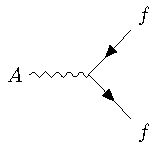
\includegraphics[width=\halffig]{figures/feyn_aff.pdf}
\caption{A Feynman diagram representing the interaction of the $A$ field with a generic fermion, $f$.} 
\label{fig:feyn_aff}
\end{figure}


\subsection{$SU(2)\times U(1)$ and the Electroweak Force}

The full picture of the electroweak section of the \ac{SM} is more complicated than the simplified explanation of the electromagnetic piece described above. 
In practice, it is necessary to consider the entire $SU(2)\times U(1)$ symmetry together, but the procedure is the same.
Enforcing the symmetry on the Lagrangian requires the introduction of a covariant derivative, this time with four total distinct terms, one for each of the generators of $SU(2)\times U(1)$.
The result is a series of terms in the Lagrangian which describe the interaction of a fermion with four vector fields, the $W_1$, $W_2$, $W_3$, and $B$ fields.
These fields can mix in the quantum sense, and linear combinations form the $W^+$, $W^-$, $Z$, and $A$ fields that are considered actual particles in the \ac{SM}\footnote{These states are the actual particles because they are mass eigenstates, but the full explanation of this will have to wait for the discussion of the Higgs mechanism.}.

\subsection{$SU(3)$ and the Strong Force}

The same procedure can be applied starting with the $SU(3)$ symmetry requirement, where eight additional fields must be introduced, one for each of the generators of $SU(3)$.
The resulting Lagrangian describes \ac{QCD} and predicts the existence of eight gauge bosons known collectively as gluons. 

\section{Noether's Theorem, Charges, and Matter}

Another direct consequence of the symmetries stipulated in the \ac{SM} are a series of conserved quantities, Noether charges, named after the mathematician and physicist Emmy Noether.
The charges arise as a direct consequence of Noether's theorem, which can be informally stated as 
\begin{quote}
\textit{For every symmetry of the Lagrangian, there exists a corresponding physical quantity whose value is conserved in time.}
\end{quote}
\noindent Or, stated another way, symmetries of the Lagrangian mathematically require the conservation of specific quantities taken from the Lagrangian. 
This relationship can also be thought of as operating in the other direction, the existence of a conserved charge can be shown to generate the symmetry in the Lagrangian.
This theorem is actually quite striking in a somewhat unexpected relation between simple geometric symmetries and physically observable conservation laws. 
For example, the theorem connects the translation invariance of the Lagrangian in space to the conservation of momentum and the translation invariance in time to the conservation of energy. 

In the context of the \ac{SM}, the required symmetries of $U(1)\times SU(2) \times SU(3)$ correspond to the charges that are considered properties of all elementary particles.
The most familiar of these properties is the electric charge, Q, which is one of the conserved quantities of $SU(2)\times U(1)$.
The remaining pieces of $SU(2)\times U(1)$ correspond to weak isospin, $T$ and $T_3$, where $T$ has only non-negative values and $T_3$ can be positive and negative.
The $SU(3)$ symmetry is generated by the three colors of \ac{QCD}, red, green, and blue, each with a corresponding opposite color, anti-red, anti-green, and anti-blue.

The matter in the observable universe consists of a collection of particles which carry these charges, in addition to spin and mass.
The particles typically thought of as matter are all fermions: particles with spin-1/2.
All of the fermions belong to one of two groups, quarks and leptons, and one of three generations.
Each of the generations have similar properties but significantly different masses; the particles in consecutive generations have increasing mass.
Quarks are distinguished from leptons in that they carry color charge, in addition to  electric charge and weak isospin.
The particles in the \ac{SM} are summarized in Figure~\ref{fig:particle_content}, and the matter particles are the twelve types of fermions displayed on the left side of the graphic.

\begin{figure}[h]
  \centering
  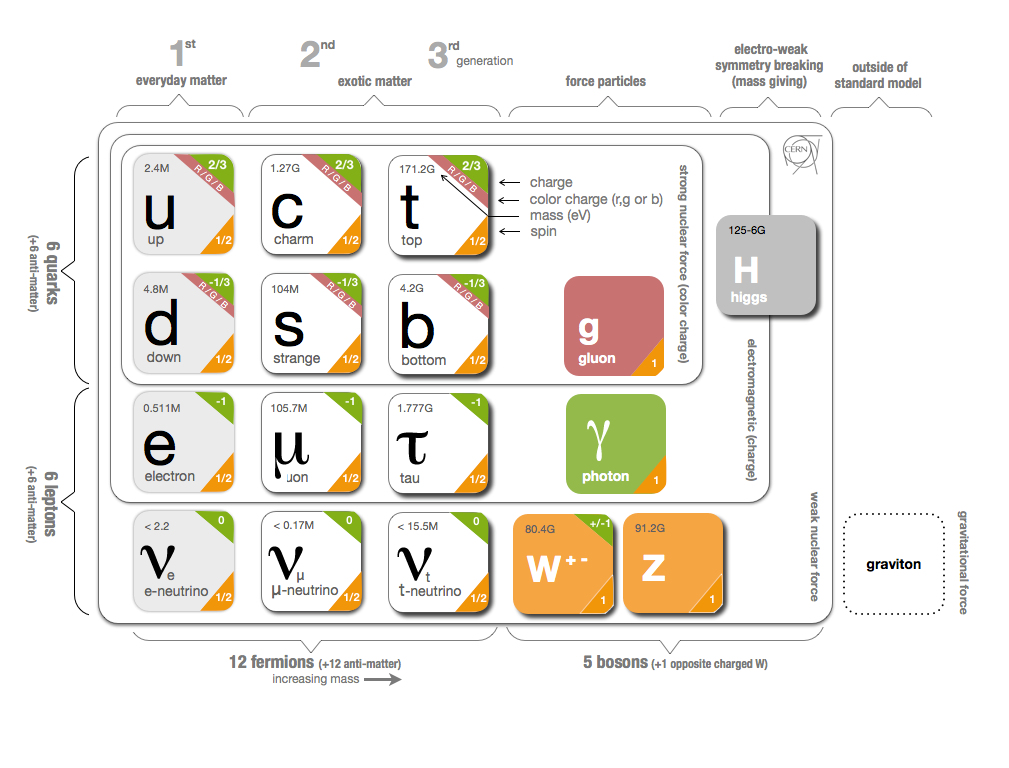
\includegraphics[width=0.9\textwidth]{figures/particle_content.png}
  \caption{The particle content of the \ac{SM}.}
  \label{fig:particle_content}
\end{figure}


\subsection{Quarks}

The three generations of quarks each have a particle with electric charge $+2/3$ and one with charge $-1/3$.
They are referred to us up and down, charm and strange, and top and bottom respectively, and these are referred to as the quark flavors.
Although Figure~\ref{fig:particle_content} only shows these six flavors, there is a unique particle for each combination of the three colors and flavor.
And each quark has an anti-particle with the opposite electric and color charge values.

However, individual quarks are never observed in nature, but instead form color-neutral bound states.
One way to form a color neutral combination is a bound state of three quarks with three different color charges, called a baryon.
Baryons are the most common type of quark configuration in conventional matter, and include protons and neutrons.
The other common configuration is a bound state of a quark and an anti-quark, called a meson, where the two quarks have the same type but opposite colors. 
The conservation of the various charges carried by quarks, along with the requirement that quarks appear in color-neutral states, result in the observed conservation of baryon number, $B$, where baryons have $B=1$ and mesons have $B=0$. 

\subsection{Leptons}

The remaining fermions, the leptons, do not carry color charge.
Each generation contains an electrically charged lepton, the electron, muon, and tau, and an electrically neutral lepton called a neutrino.
For the charged leptons, the flavors are mass eigenstates, with the masses listed in Figure~\ref{fig:particle_content}.
The flavors of the neutrinos, on the other hand, are not mass eigenstates: they propagate in mass eigenstates and so can oscillate between different flavors.
The absolute masses of the neutrinos are not currently known, but the phenomenon of oscillations shows that they have three different mass values.
Although there is no direct conservation law resulting from the symmetries of the \ac{SM} Lagrangian, no interactions have been observe which alter lepton number, $L$, the difference in the number of leptons and anti-leptons. 

\subsection{Chirality}

All of the fermions described above have two possible values of the magnitude of weak isospin, $T$, either $0$ or $1/2$.
The fermions with $T = 0$ are called right-handed, while those with $T=1/2$ are called left-handed.
For left-handed fermions, each of the quark and lepton generations have one particle with $T_3 = -1/2$ and one with $T_3 = +1/2$.
The neutrinos have $T_3 = +1/2$, while the charged leptons have $T_3 = -1/2$.
Similarly, the positively charged quarks have $T_3 = +1/2$ and the negatively charged quarks have $T_3 = -1/2$.
Because the right-handed neutrinos would have no charge of any type, it is not clear if they exist at all.


\section{Higgs Mechanism and Mass}

The description of the electroweak forces above left out an important part of the observed nature of the electroweak force.
Many physical experiments observed phenomena corresponding to the interaction of the weak bosons that were best explained if they had significant masses.
A large mass for the W and Z bosons would explain the relative weakness of their interactions compared to the electromagnetic field.
The Lagrangian's discussed above did not include a mass term for the gauge bosons, and in fact such a term would not be allowed by the requirement of gauge invariance. 
This was a significant problem for the \ac{SM}, and the symmetry of the electroweak sector would have to be broken in order to allow for non zero masses for some of the gauge bosons.

One mechanism to allow for this spontaneous symmetry breaking is the Higgs mechanism, which posits the existence of an additional scalar field.
It begins with a $SU(2)\times U(1)$ invariant Lagrangian of the form 

\begin{equation}
  \mL = |D_\mu\phi|^2 - \frac{1}{2}\mu^2\phi^+\phi - \frac{1}{4}\lambda(\phi^+\phi)^2
\end{equation}

\noindent where $\phi$ is the new scalar field and, importantly, $\mu^2$ is negative.
This leads to a minimum value of the field at a non-zero value of $\phi$, specifically where

\begin{equation}
 \langle \phi \rangle = \frac{1}{\sqrt{2}} \begin{pmatrix}0\\v\end{pmatrix} \quad \mathrm{with} \quad v = \frac{2\mu^2}{\lambda}
\end{equation}

\noindent Expanding the original Lagrangian about its expectation value, 

\begin{equation}
  \langle \phi \rangle = \frac{1}{\sqrt{2}} \begin{pmatrix}0\\v + H\end{pmatrix}
\end{equation}

\noindent gives potential terms in the Lagrangian like 

\begin{equation}
  \mL_{H} = -\frac{1}{2}m_H^2 H^2 - \sqrt{\frac{\lambda}{2}}m_H H^3 - \frac{1}{4}\lambda H^4
\end{equation}

\noindent where $m_H = \sqrt{2}\mu$.
The form of this Lagrangian shows that the non-zero expectation value of the $\phi$ field has introduced a massive scalar field $H$ with self interaction terms.
It has an additional important consequence on the description of the gauge bosons, through the expansion of the term involving the covariant derivative:

\begin{equation}
  |D_\mu\phi|^2 \supset \frac{1}{8}\left(g^2(W_{1\mu}W_1^\mu + W_{2\mu}W_2^\mu) + (g'B_\mu - gW_3{\mu})^2\right)
\end{equation}

where the $W_i$ and $B$ fields are the original $SU(2)\times U(1)$ gauge fields mentioned previously.
The above equation can be rearranged using linear combinations of the fields to from mass terms for the gauge bosons, and the mass eigenstates are exactly the $W^\pm$, $Z$, and $A$ fields.
Only the $A$ field, corresponding to the photon, results in a zero mass, and the remaining three fields acquire masses.
Because the originally introduced Lagrangian, written in terms of $\phi$, was clearly gauge invariant, this resulting configuration must also be gauge invariant.

This is the Higgs mechanism, where the introduction of a gauge invariant scalar field with a non-zero expectation value can generate masses for the gauge bosons without violating the underlying symmetries.
The particle that is associated with the perturbations of this field, $H$, is called the Higgs boson, and is said to generate the masses of the remaining bosons.
The resulting masses are listed in Figure~\ref{fig:particle_content}.
Because this mechanism was so successful in describing the observed properties of the $W$ and $Z$ bosons, it has been considered part of the \ac{SM} for decades, although the actual Higgs boson was only recently observed in 2012, confirming the theory.

The Higgs mechanism is also responsible for generating the masses of the fermions.
The original mass terms that were listed in the Lagrangian for fermions are replaced with Yukawa coupling terms, which introduce interactions between the $\phi$ field and the fermions.
Like with the gauge bosons, the non-zero expectation value of the field yields mass terms, and the expansion about that value introduces interaction terms between the fermions and the Higgs boson.
The masses are different between each fermion because each has a different Yukawa coupling, which results in the masses listed in Figure~\ref{fig:particle_content}.

\section{Phenomenology}

The \ac{SM} Lagrangian described above contains all of the information necessary to describe particle physics through the path integral formulation. 
However, a tremendous amount of complexity emerges from that description because of the diverse allowed interactions between the ensemble of particles in the \ac{SM}.
A qualitative understanding of the phenomenology produced by those interactions is immensely helpful in understanding the analysis of particle physics.

\subsection{Electroweak Physics}

The masses of the $W$ and $Z$ bosons result in significantly different processes for the weak fields than the electromagnetic field, despite their interactions being similar before symmetry breaking.
The massless photon is stable, and can propagate in a vacuum, resulting in the familiar long range interactions of electromagnetism.
The $W$ and $Z$ bosons, however, are unstable, as they have large enough masses to decay to fermions, such as the decays shown in Figure~\ref{fig:feyn_weak}.
For this reason, photons can be observed directly, while the other bosons are sufficiently short-lived that they can only be measured from their decay products.

\begin{figure}
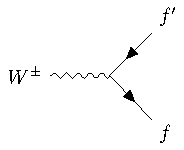
\includegraphics[width=\halffig]{figures/feyn_wdecay.pdf}
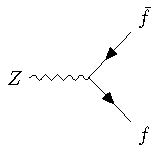
\includegraphics[width=\halffig]{figures/feyn_zdecay.pdf}\\
\caption{The Feynman diagrams representing the decays of the W and Z bosons to fermions. Here $f$ indicates a generic fermion, $\bar{f}$ its antiparticle, and $f'$ the partner of that fermion in the same generation.}
\label{fig:feyn_weak}
\end{figure}

Because the $W$ and $Z$ bosons interact with both quarks and leptons, they are responsible for the production of leptons in proton-proton collisions.
$Z$ bosons produce pairs of opposite sign, same flavor leptons.
$W$ bosons, on the other hand, produce a single lepton and the corresponding neutrino.

\subsection{Strong Physics}

The phenomenology of the strong sector differs significantly from the weak sector because the gluons are massless but color charged.
Because of this, gluons can interact with each other, and contributions from multiple gluon interactions lead to a significant growth in the strength of the field at low energies.
The dependence of the field strength on the energy scale is described by renormalization, and in \ac{QCD} the coupling is only small at high energies.
Above around the \GeV scale, the interactions of quarks become perturbative, similar to the electroweak fields; this phenomenon is known as asymptotic freedom.

At lower energies, however, the strength of the strong interaction is so significant that the interactions of color-charged particles create additional particles until they form neutral bound-states.
This process is known as hadronization, and explains why no quarks are observed isolated in nature: they all form bound states of hadrons like protons, neutrons, and pions.
The hadronization process can produce a significant number of particles, so that a single energetic quark recoiling against another quark can generate a cascade of dozens of hadrons.
Because of the initial boost of such an energetic configuration, the resulting hadrons are collimated, and conical spray of particles often referred to as a jet.

\subsection{Proton-Proton Collisions}

Proton-proton collisions are a convenient way to generate high energy interactions to probe the \ac{SM} and to search for new physics.
At the energies that will be discussed in this analysis, the substructure of the protons is very important to the description of the resulting interactions.
At lowest order, protons are composed of two up quarks and one down quark, but this description is incomplete.
The actual bound state includes a chaotic sea of additional quarks and gluons, each of which carries a variable fraction of the proton's energy.
When a proton-proton collision takes place, it is these constituents that interact with each other, resulting in a highly variable collision energy even when the proton-proton energy is consistent.

The fraction of the energy carried by each constituent varies moment to moment, but can be modelled probabilistically by \acp{PDF}.
These are difficult to predict theoretically, as the \ac{QCD} calculations are extremely complex, and instead are measured in hard-scattering experiments.
They are usually represented by how often a given type of particle carries a fraction $x$ of the total proton energy.
Those fraction change significantly with the scale of the interaction; the \acp{PDF} of proton-proton collisions at both $Q^2 = 10$ \GeV\tsup{2} and $Q^2 = 10^4$ \GeV\tsup{2} are shown in Figure~\ref{fig:pdfs}.

\begin{figure}
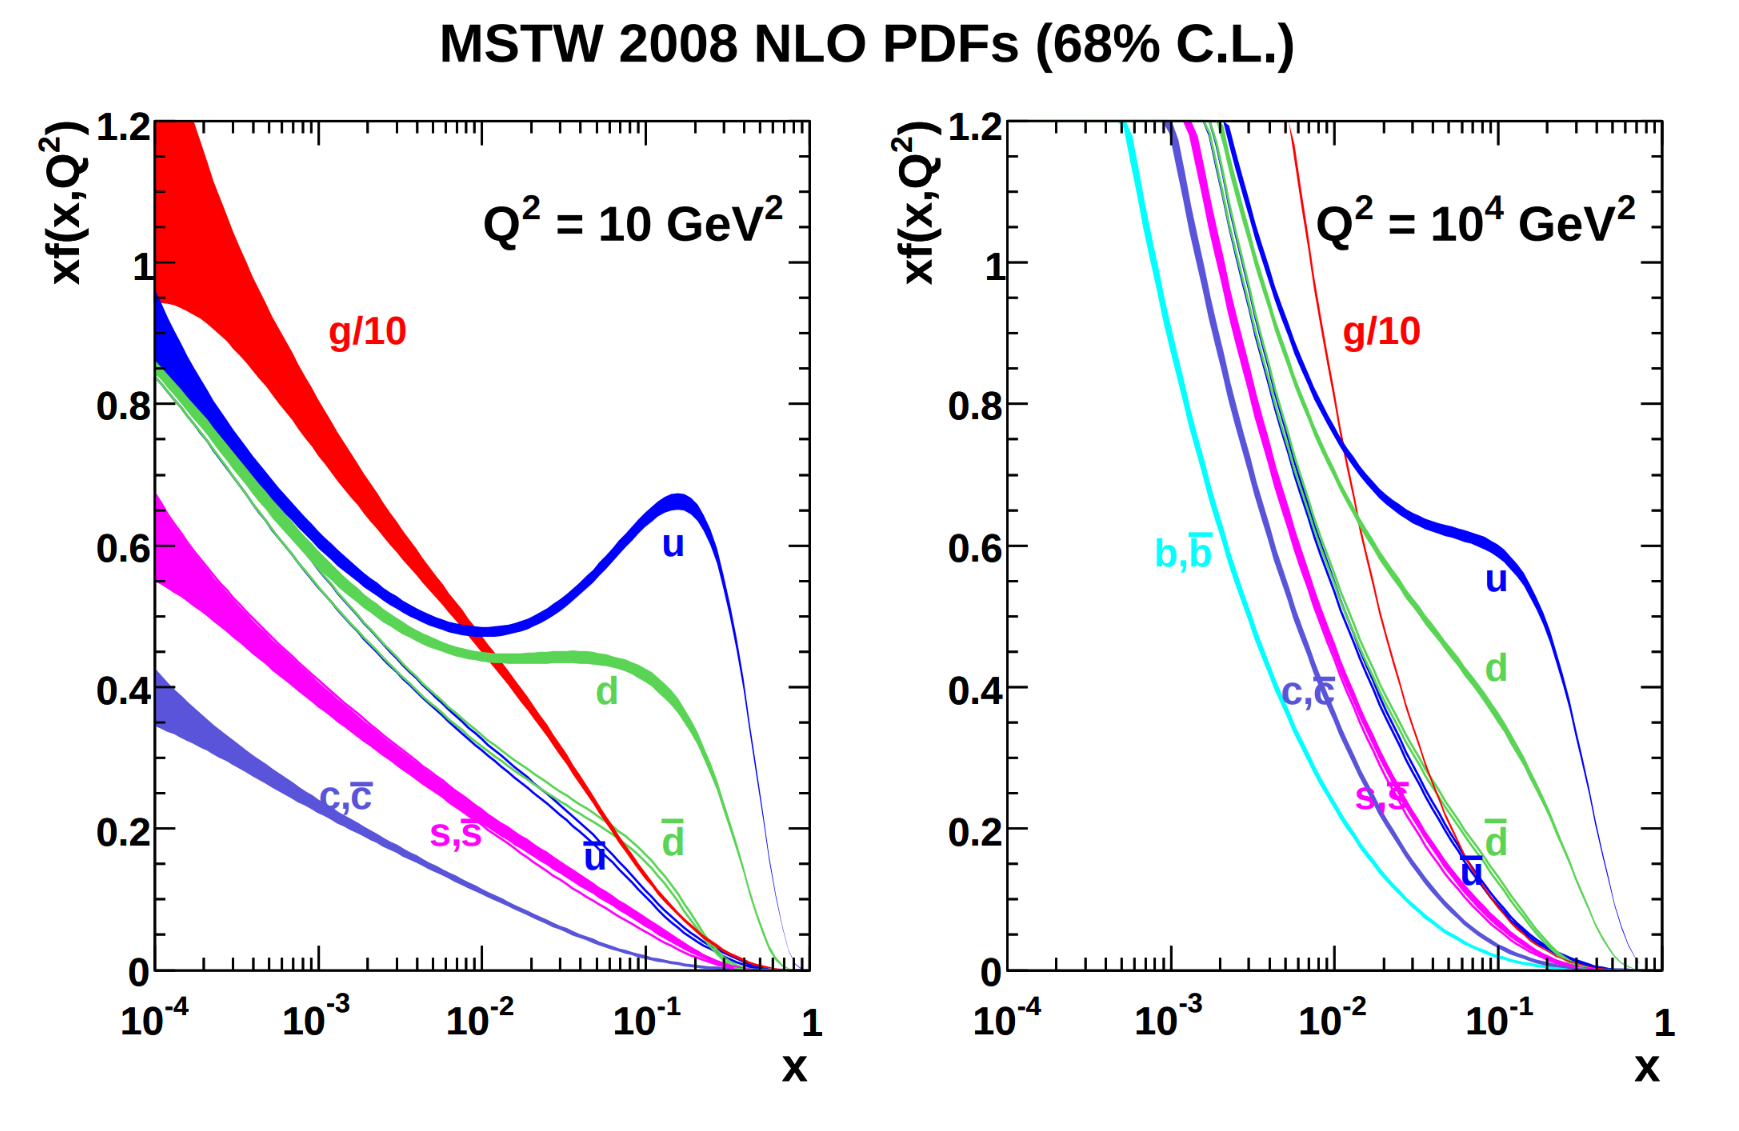
\includegraphics[width=\fullfig]{figures/pdfs.png}
\caption{The \acp{PDF} for proton-proton collisions at $Q^2 = 10$ \GeV\tsup{2} and $Q^2 = 10^4$ \GeV\tsup{2}. Each shows the fraction of particles which carry a fraction $x$ of the total proton energy at the specified scale~\cite{pdfs}.}
\label{fig:pdfs}
\end{figure}


\section{Limitations}
\label{sec:limitations}

Despite the great success of the relatively simple \ac{SM} in describing such a broad range of emergent phenomena, it is clear that the picture it presents of the interactions of fundamental particles is incomplete.
The \ac{SM} contains concerning coincidences that suggest a more ordered underlying substructure that is not expressed in the current form.
It also fails to explain a number of cosmological measurements of the nature of matter in the universe.
These limitations suggest the need for new, \ac{BSM} physics that would provide a more complete description at higher energies.


\subsection{Theoretical Concerns}

There have been no successful integrations of the \ac{SM}'s description of the electroweak and strong forces with the description of gravity, and it is still unclear how to account for the effects of gravity at the Plank scale of approximately $10^{19}$ \GeV, where it can no longer be ignored. 
The Plank scale is an important cutoff for the \ac{SM}, as it is clear that the \ac{SM} must break down somewhere between the current highest energy tests of the \ac{SM}, around 1 \TeV, and the Plank scale.

One example of this is the Higgs mass, which is determined in the \ac{SM} by a sum of it's bare mass and the interactions in the vacuum with all massive particles.
As their must be new physics at the Plank scale to describe gravity, some of those corrections would include contributions at a scale seventeen orders of magnitude above the mass of the Higgs.
Either the bare mass of the Higgs boson precisely cancels those contributions to leave a remainder seventeen orders of magnitudes smaller, or a new theory exists at a lower scale the shields the Higgs mass from those terms.
A theory where such a unlikely cancellation of free parameters occurs is called fine-tuned, and one that is free from such cancellations is called natural.
Theories where the mass of the Higgs is natural are usually preferred, as the suggest an underlying, coherent structure.

There is also a compelling argument that the $SU(3)\times SU(2) \times U(1)$ gauge structure of the \ac{SM} might originate from a single, unified gauge theory.
For example, it is possible to represent that gauge structure as a $SU(5)$ gauge group with only a few inconsistencies with the current implementation.
This unification is suggested by the scaling of the coupling constants for each of the forces under renormalization, they come close to converging to a single value at higher energies, as seen in Figure~\ref{fig:unification_sm}. 
An additional correction to the scaling of the coupling constants from new physics above the \TeV scale could cause them to merge into a single value at high energies. 

\begin{figure}
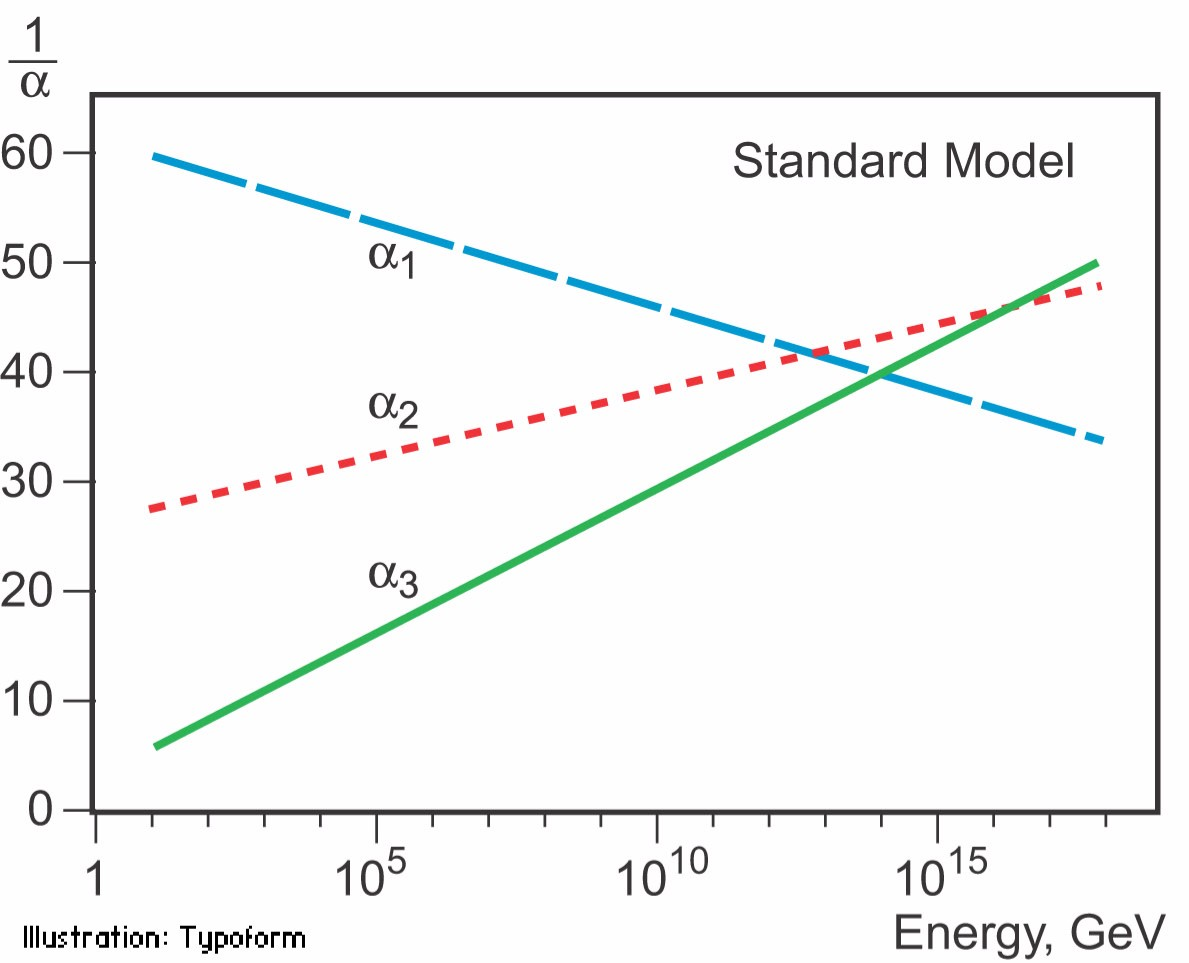
\includegraphics[width=\fullfig]{figures/unification_sm.jpg}
\caption{An approximation of the running of the coupling constants in the \ac{SM} up to the Planck scale~\cite{unification_plot}.}
\label{fig:unification_sm}
\end{figure}

\subsection{Cosmological Observations}

The \ac{SM} contains a symmetry in the description of matter and antimatter that is not reflected in cosmological observations.
The process of the standard model create or remove matter and antimatter in equal amounts, so a universe that begins with an equal quantity of each should result in a universe with an approximate balance of matter and antimatter.
However, cosmological observations of the relative amount of each type clearly show that the directly observable mass of the universe is overwhelmingly made of matter.
As this difference is largely a difference in the generation of baryons and anti-baryons, this discrepancy is often referred to as the baryogenesis problem.

A number of astrophysical observations of large scale gravitational interactions suggest the presence of a significant amount of non-luminous matter that interacts with the normal matter only gravitationally.
The first evidence of this came from the observation of galactic rotation curves, the velocities of stars as a function of the radius from the center of a galaxy.
These can be directly predicted from the amount of matter contained within the sphere up to the radius of the star.
An estimate based only on the luminous matter in the galaxies would predict a dependence that falls off with the radius, but the observed curves show a mostly constant distribution of velocities~\cite{rotation_curves}, as seen in Figure~\ref{fig:rotational_curve}.
The higher velocities than predicted by the luminous matter can be explained by a halo of dark matter that extends significantly outside the galactic disk.

\begin{figure}
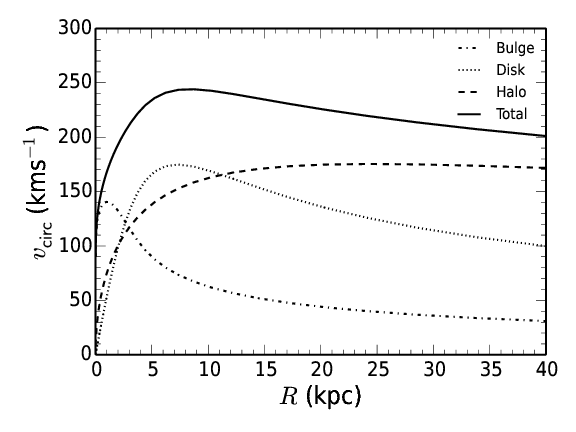
\includegraphics[width=\fullfig]{figures/rotation_curves.png}
\caption{The distribution of velocities of stars as a function of the radius from the center of the galaxy. The contributions to the velocity from the various components of matter in the galaxy are shown~\cite{rotation_curves}.}
\label{fig:rotational_curve}
\end{figure}

This dark matter accounts for a majority of the matter in the universe, and is incompatible with the matter particles predicted by the \ac{SM}.
Many observations support its existence, but there have been no direct detections of a particle which could account for the large quantity of gravitationally interacting dark matter.
The \ac{SM} would have to require a significant extension to include the particles needed to explain dark matter and the processes needed to explain the observed matter-antimatter asymmetry. 

\chapter{Supersymmetry}

\label{ch:supersymmetry}
% --------------------------------------------------------------------------------

The theory of \ac{SUSY} presents an extension to the \ac{SM} that solves a number of the outstanding issues. 
It is based an another proposed symmetry, one which introduces an equality between the fermionic particles and proposed bosonic partners and also between bosonic particles and their proposed fermionic partners.
The symmetry is defined by extending spacetime into a superspace, which includes one dimension that describes a particle's spin: a transformation in this space moves a fermion with spin-1/2 to a boson with spin-0 or vice-versa.
Requiring the \ac{SM} to be symmetrical under these transformations requires the existence of a bosonic partner for every current matter fermion in the \ac{SM} and a fermionic partner for every boson. 
The partners are called superparticles (sparticles), where quarks partner with squarks and leptons partner with sleptons, and each boson has a fermionic partner called a gaugino.
The superpartners, in the original form of the theory, should be identical to the original particle in every way except for spin; that is they would have the same quantum charges and the same mass.

However, the simplest version of the theory, where the symmetry is unbroken, is incompatible with current observations of physics in a number of systems.
The most striking example comes from the electron, as the superpartner of an electron would introduce a stable, negatively charged, and bosonic particle. 
Such a particle would drastically alter atomic properties by providing a way to create atoms without the valence structure of electrons that results from the Pauli exclusion principle for fermions.
Various high energy physics measurements have also confirmed the spin of the W and Z bosons, for example, and a fermionic gaugino has never been produced at those masses.
The solution to this incompatibility with observation is to conjecture that the symmetry exists but is spontaneously broken, where the masses of the supersymmetric particles are significantly larger than those of the current \ac{SM} particles.
Like the spontaneous symmetry breaking of the electroweak system, this symmetry breaking can be accomplished by introducing an additional Higgs mechanism.

% ----------------------------------------

\section{Structure}
\label{sec:mssm}

There are a number of ways to model the particulars of \ac{SUSY}, but many of the resulting phenomena are similar, and a discussion of an example is sufficient describe the structure and results of the theory.
The \ac{MSSM} is one example of a complete description that includes the necessary symmetry breaking to result in the different masses between particles and sparticles~\cite{mssm}.
It is called minimal because it is designed to use the simplest possible extension to the \ac{SM} that incorporates \ac{SUSY}.
However even a minimal version includes a remarkable number of free parameters, over 100, and the \ac{MSSM} is often further constrained to include fewer parameters in models such as the \ac{pMSSM} and the \ac{cMSSM}~\cite{pmssm}.

The theory includes a sparticle partner for every \ac{SM} particle, which are listed in Table~\ref{tab:sparticles}.
To then provide the different masses for those sparticles, the \ac{MSSM} introduces a second Higgs interaction.
The resulting scalar field, along with the original Higgs field, generates five total particles, $h^0$, the original Higgs boson, $A^0$, $H^0$, and $H^\pm$, where the last two are electrically charged.
These Higgs bosons can mix with the supersymmetric gauginos to form a series of mass eigenstates.
These are usually referred to by the order of their masses, where the neutral gauginos (neutralinos) are labeled $\tilde{\chi}_1^0$, $\tilde{\chi}_2^0$, $\tilde{\chi}_3^0$, and $\tilde{\chi}_4^0$. 
The charged gauginos (charginos) are similarly labeled $\tilde{\chi}_1^\pm$ and $\tilde{\chi}_2^\pm$. 
Table~\ref{tab:sparticles}, lists the gauginos which are direct partners of the original gauge bosons in the \ac{SM} rather than these resulting mass eigenstates.

\begin{table}
\centering
\begin{tabular}{lcc}
\hline
Sector & Particles & Sparticles \\
\hline
Baryonic Matter & $(u,d)$ & $(\tilde{u},\tilde{d})$ \\
                & $(c,s)$ & $(\tilde{c},\tilde{s})$ \\
                & $(t,b)$ & $(\tilde{t},\tilde{b})$ \\
Leptonic Matter & $(\nu_e,e)$ & $(\tilde{\nu_e},\tilde{e})$ \\
                & $(\nu_\mu,\mu)$ & $(\tilde{\nu_mu},\tilde{\mu})$ \\
                & $(\nu_\tau,\tau)$ & $(\tilde{\nu_\tau},\tilde{\tau})$ \\
Higgs           & $(H_u^+, H_u^0)$ & $(\tilde{H}_u^+, \tilde{H}_u^0)$ \\
                & $(H_d^0, H_d^-)$ & $(\tilde{H}_d^0, \tilde{H}_d^-)$ \\
Strong          & $g$ & $\tilde{g}$ \\
Electroweak     & $(W^\pm, W^0)$ & $(\tilde{W}^\pm, \tilde{W}^0)$ \\
                & $B^0$ & $\tilde{B}^0$ \\
\end{tabular}
\caption{The particles in the \acs*{SM} and their corresponding superpartners in the \acs*{MSSM}.}
\label{tab:sparticles}
\end{table}


In addition to the new particle content, the \ac{MSSM} introduces new interactions for the gauge bosons and gauginos.
All interaction terms are added to the Lagrangian which describe the interaction of a gauge boson or gaugino with a particle or sparticle with the appropriate charge.
Such terms include a few interactions which would violate the observed $B - L$ symmetry that prevents proton decay.
Either the couplings on these terms must be extremely small to match the experimental limits on those decays, or an additional symmetry must be imposed to exclude the terms.
The \ac{MSSM} and several other \ac{SUSY} models choose to introduce a new symmetry known as R-parity, where the conserved quantity, $P_R$ is defined as
\begin{align*}
P_R = (-1)^{2s + 3(B-L)}
\end{align*}
with $s$ as the spin of the particle.
Sparticles are R-parity odd while \ac{SM} particles are R-parity even.
And by requiring that each term in the supersymmetric Lagrangian conserves R-parity, it is enforced that sparticles are produced in pairs.

The conservation of R-parity removes the $B-L$ violating terms from the Lagrangian.
The remaining terms include all of the interactions of the \ac{SM} where two of the particles are replaced with their \ac{SUSY} partners, so that R-parity is conserved in the interactions.
This also has an important significance in making the \acf{LSP}, the $\tilde{\chi}_1^0$, stable, as it cannot decay to only \ac{SM} particles without violating the conservation of R-parity.
The heavier sparticles then decay in chains, emitting an \ac{SM} particle in each step, and leave behind the \ac{LSP} at the end of the chain.

\section{Motivation}

\ac{SUSY} models, including the \ac{MSSM}, ameliorate many of the issues in the \ac{SM} discussed in Section~\ref{sec:limitations}.
\ac{SUSY} is particularly well motivated as a natural extension to the \ac{SM} because the simple underlying assumption solves three major, seemingly unrelated concerns.
And these benefits all require that at least some of the sparticles exist at the \TeV scale, within the reach of modern collider experiments.

The first, a solution to the hierarchy problem, comes as a direct consequence of the introduction of massive superpartners for each \ac{SM} particle.
The contributions to the Higgs mass from the much higher energy Planck scale come from a series of loop diagrams in the \ac{SM}, where each massive \ac{SM} particle has a loop contribution.
The introduction of superpartners generates a series of corresponding diagrams for correction to the Higgs mass, with opposite sign contributions because the superpartners have different spins.
Those opposite sign contributions cancel the divergences from the original loop diagrams at high energies, leaving behind a correction to the Higgs mass that is at the same scale as the masses of the superpartners. 
If the superpartners exist at the \TeV scale, then the Higgs mass of 125 \GeV can be explained without significant fine-tuning, and the theory becomes natural.

\ac{SUSY} also has the potential to precisely enable the unification of the coupling constants at high energy.
Without supersymmetric contributions, the coupling constants come close to a single value near the Planck scale suggesting an underlying trend, as shown in Figure~\ref{fig:unification_sm}, but they do not exactly merge.
With the addition of the \ac{MSSM}, they can join almost exactly at a single point, enabling a unification into a single gauge theory at high energy, as shown in Figure~\ref{fig:unification_susy}. 
This precise unification, like the naturalness argument, also requires that the masses of the superpartners be near the \TeV scale.

\begin{figure}
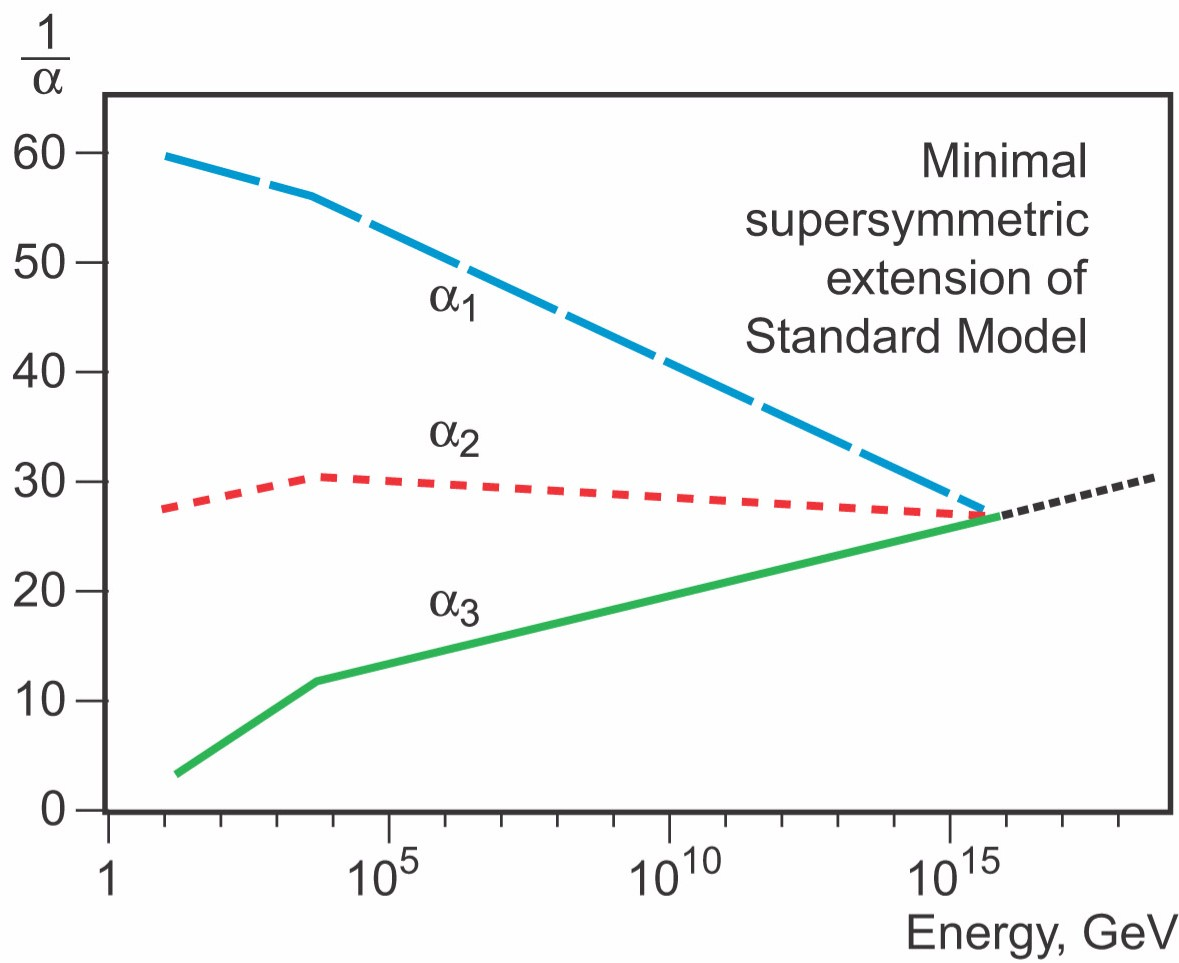
\includegraphics[width=\fullfig]{figures/unification_susy.jpg}
\caption{An approximation of the running of the coupling constants in the \acs*{MSSM} up to the Planck scale~\cite{unification_plot}.}
\label{fig:unification_susy}
\end{figure}

The presence of R-parity in a \ac{SUSY} model also provides an explanation for dark matter.
The \ac{LSP}, as discussed in Section~\ref{sec:mssm}, is a massive, neutral, and stable particle as long as R-parity is conserved.
In the early universe, when the energy density was extremely high, \acp{LSP} could be spontaneously produced just as often as other particles like photons, and would result in a thermal equilibrium.
Then, as the universe cooled, the average energy would be too low to create additional \acp{LSP}, and they would be left behind and only interact with the remaining matter gravitationally, a process called freeze out.
Since those particles are stable, they would remain indefinitely. 
With the existence of an \ac{LSP} at around the \TeV scale, this process can explain the observed amount of dark matter in the universe.
A \ac{WIMP}, exactly what is proposed in the \ac{LSP}, provides the correct interaction rate to predict the currently observed ratio of dark matter to baryonic matter.

Together, this variety of solutions to existing problems provides strong theoretical support for the existence of \ac{SUSY} near the \TeV scale.
The \ac{LHC} is the first collider experiment to be able to probe into \TeV scale interactions, providing a new opportunity to search for this extension to the \ac{SM}.
A range of models have begun to be excluded with masses above 1 \TeV~\cite{pdg}, leading to a motivation to explore a wider variety of models with phenomena that may have been missed by the most direct search strategies.

\section{Simplified Models}

The \ac{MSSM} is just one example of a large suite of \ac{SUSY} models with similar results.
Each of those models can have hundreds of individual parameters that ultimately determine the masses and interactions of the supersymmetric particles.
To avoid this complexity in making experimental measurements, the analyses of high energy collisions often rely on simplified models.
These models focus on a single process predicted by a theory, and the observable parameters such as the mass of the particles and their lifetimes are controlled directly, rather than tuning the hundreds of underlying parameters.
This allows straightforward simulation of a specific event topology with control over the parameters that most directly influence the experimental signatures.

Experimental analyses use these models to search for new physics and to set limits on the production rates for a given type of process with working points of a few observable parameters.
As one example, a simplified model may specify pair production of gluinos where the free parameters are the mass of the gluino and the types and masses of the particles it can decay into.
The small number of parameters allows the phase space to be searched in a grid by simulating events with a few examples for the parameters and interpolating between them.
The resulting analysis can set cross sectional limits as a function of the simplified parameters, and this allows for an easy interpretation of the result in a number of \ac{SUSY} models.

\section{Long-Lived Particles}
\label{sec:llp_theory}

Some proposed \ac{SUSY} models can produce \acp{LLP} other than just the \ac{LSP}.
The most direct search strategies for \ac{SUSY} often assume that the various non-stable sparticles decay promptly, rather than propagating through some fraction of the detector.
Although the processes involved are very similar, the long-lifetime of the produced particles can lead to very different experimental signatures, and often require separate dedicated searches.
It is important to design and execute search strategies for \acp{LLP} in order to completely cover possible production of new physics. 

There are a several ways to generate long lifetimes for the massive \ac{SUSY} particles, depending on the specific model.
In examples like Spread Supersymmetry~\cite{spreadsusy} and Split Supersymmetry~\cite{split1,split2}, the introduction of a split between two mass scales suppresses the decay of gluinos.
In these and similar models, the squarks are much heavier than the gluino, where the mass scale of the squarks is roughly $10^6$ \GeV while the mass scale of the gluinos is roughly $10^3$ \GeV.
The gluino must decay through the production of a virtual squark, as shown in the diagram of Figure~\ref{fig:gluino_decay}.
The large mass of the squarks in the split models suppresses the decay rate, and can result in lifetimes of the order of 1 ns~\cite{spreadsusy}.

\begin{figure}
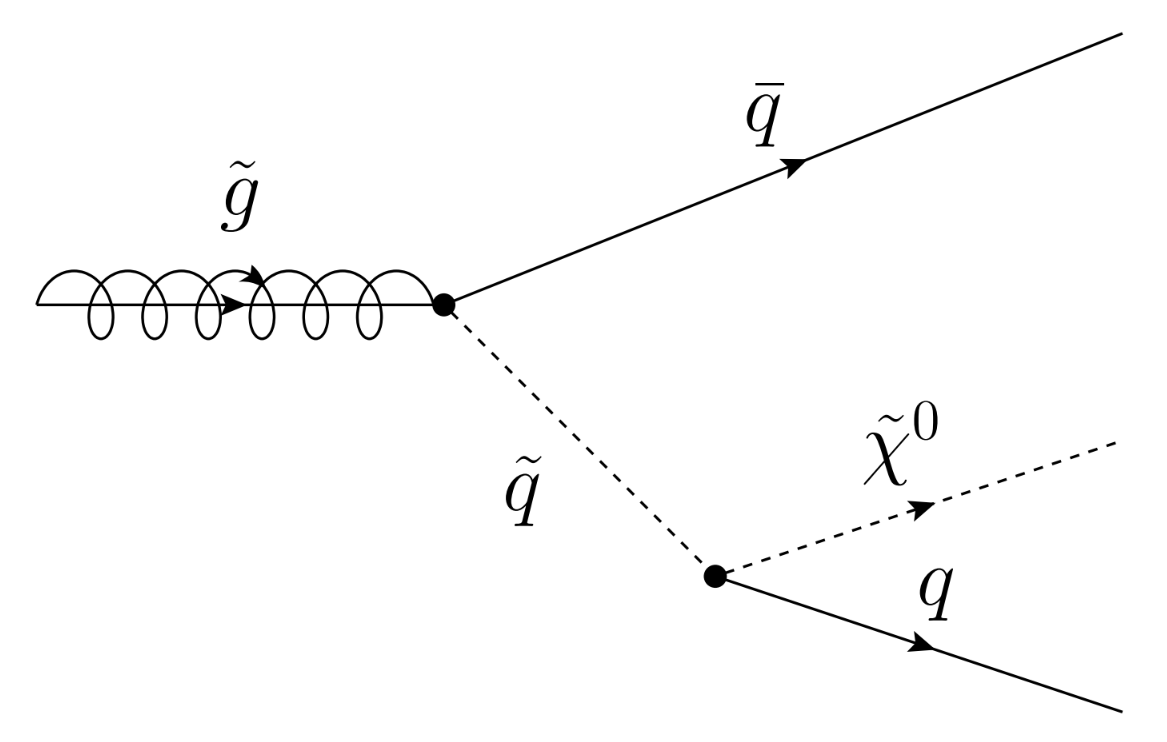
\includegraphics[width=\fullfig]{figures/gluino_decay.png}
\caption{The decay of a gluino to quarks and an \acs*{LSP}, which precedes through a squark.}
\label{fig:gluino_decay}
\end{figure}

Nearly degenerate particles can also result in long lifetimes, again by suppressing decay rates.
When a particle must decay to another particle with nearly the same mass, the phase space factor in the decay results in a low decay rate.
For example, a neutron has a lifetime of roughly fifteen minutes because its mass is so close to the proton.
Models which result in a nearly degenerate chargino and \ac{LSP} provide a long-lived chargino as well.

Again, because of the wide variety of models which can produce \acp{LLP} and the large number of parameters which determine their masses and lifetimes, the analysis presented here focuses on simplified models rather than assuming any particular underlying theory.
The models directly specify the decay mode of the \acp{LLP} as well as their masses and lifetimes, using a grid of values.
The results of searches using these simplified models can be interpreted over a very wide range of models that predict \acp{LLP}, even including non-supersymmetric extensions to the \ac{SM}.

%\chapter{Long-Lived Particles}

\label{ch:longlived}
% --------------------------------------------------------------------------------

\section{Mechanisms}

\subsection{Examples in Supersymmetry}

% ----------------------------------------

\section{Phenomenology}

\subsection{Disimilarities to Prompt Decays}

\subsection{Characteristic Signatures}

% ----------------------------------------


%\ctparttext{You can put some informational part preamble text here.}
\part{Experimental Structure and Reconstruction}
\label{part:experiment}
\chapter{The Large Hadron Collider}

\label{ch:lhc}
% --------------------------------------------------------------------------------

The \ac{LHC}, a two-ring superconducting hadron accelerator, provides high energy proton-proton collisions for several large experiments at \ac{CERN} in Geneva, Switzerland~\cite{lhc_machine, lhc_guide}. 
It is the largest, highest-luminosity, and highest-energy proton collider ever built, and was constructed by a collaboration of more than 10,000 scientists from the more than 100 countries that contribute to \ac{CERN}.
The original design of the \ac{LHC} focused on providing collision energies of up to 14 \TeV and generating enough collisions to reveal physics beyond the \ac{SM} which is predicted to exist at higher energy scales.

The \ac{LHC} was installed in an existing 27 km tunnel at \ac{CERN} which was originally designed to house \ac{LEP}~\cite{lep_tdr}.
This allows the collider to use existing accelerators at the same complex to provide the initial acceleration of protons up to 450 \GeV before injecting into \ac{LHC}.
The injected hadrons are accelerated up to as much as 14 \TeV while being focused into two beams traveling in opposite directions.
During this process the protons circulate around the tunnel millions of times, while the beams are intermittently crossed at the four locations of the experiments to provide collisions.
These collision points correspond to the four major \ac{LHC} experiments: \ac{ATLAS}, \ac{CMS}, \ac{LHCb}, and \ac{ALICE}, and Figure~\ref{fig:cern_locations} shows the layout of the experiments both on the surface and below.
\ac{ATLAS} and \ac{CMS} are both general purpose, high-luminosity detectors which search for a wide range of new types of physics~\cite{atlas_experiment, cms_experiment}.
\ac{LHCb} studies the interactions of b-hadrons to explore the asymmetry between matter and antimatter~\cite{lhcb_experiment}.
\ac{ALICE} focuses on the collisions of lead ions, which the \ac{LHC} also provides, in order to study the properties of quark-gluon plasma~\cite{alice_experiment}.

\begin{figure}
\centering
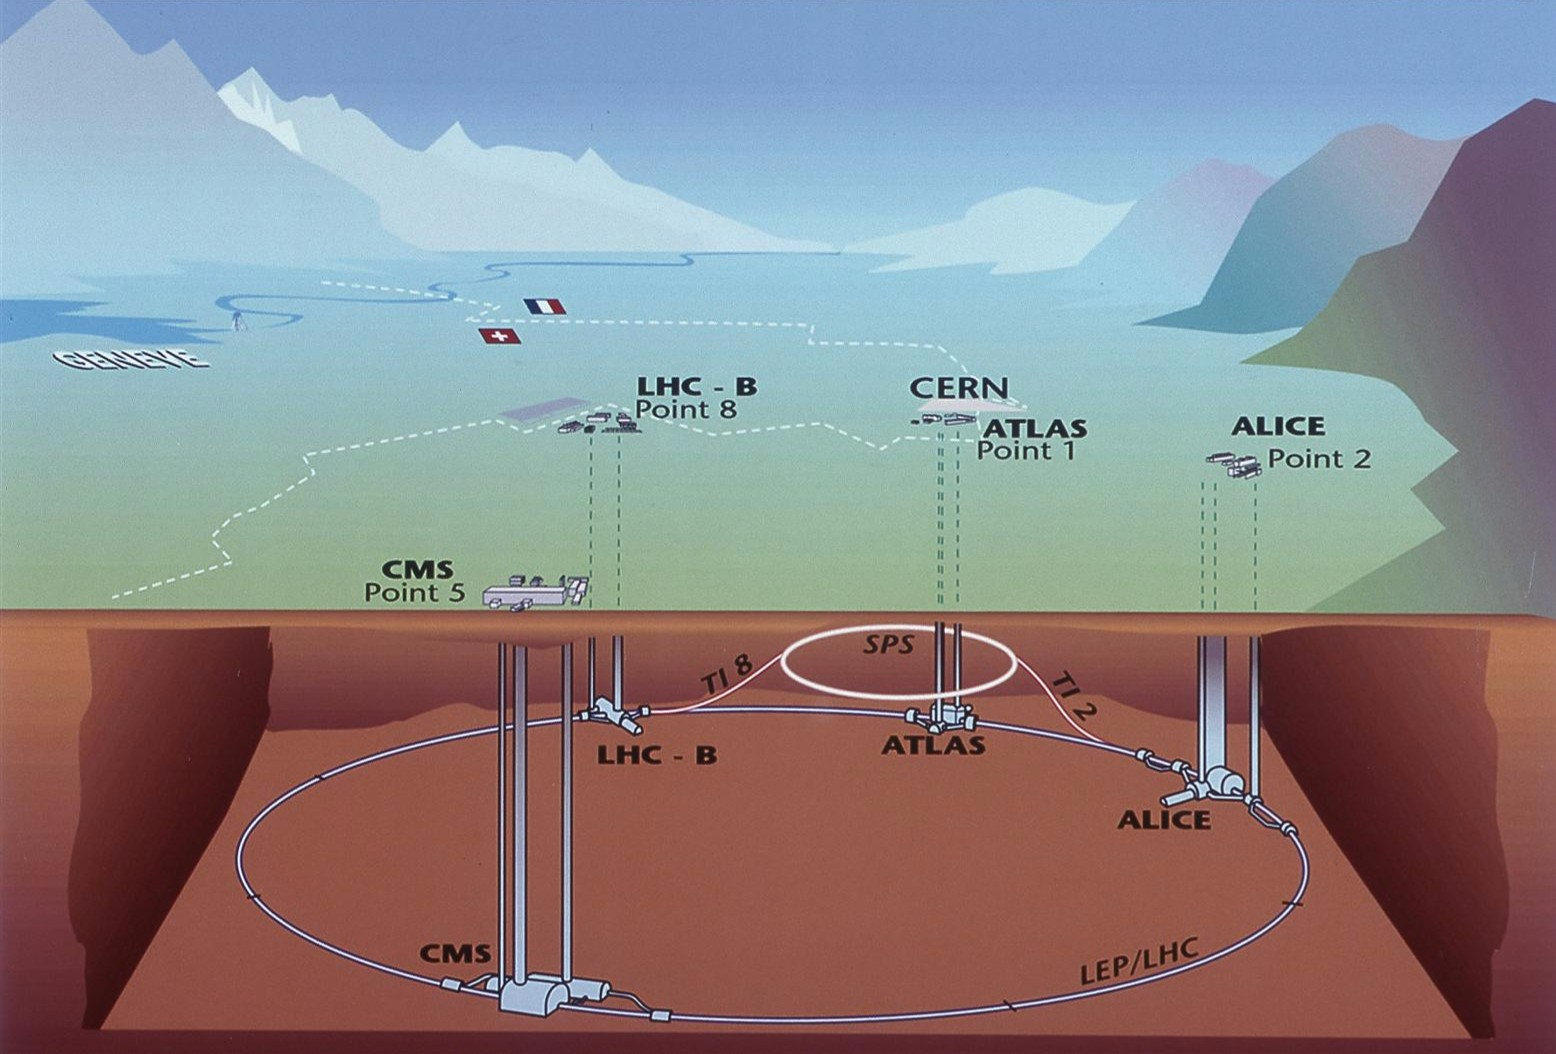
\includegraphics[width=\fullfig]{figures/cern_locations.jpg}
\caption{The four collision points and corresponding experiments of the \ac{LHC}. The image includes the location of the nearby city of Geneva as well as the border of France and Switzerland.}
\label{fig:cern_locations}
\end{figure}

During the first five years of continued operation, after the \ac{LHC} turned on in 2010, the \ac{LHC} has provided four major data collecting periods.
In 2010 the \ac{LHC} generated collisions at several energies, starting at 900 \GeV. 
It increased the energy from 900 \GeV to 2.76 \TeV and then subsequently to 7 \TeV, with a peak luminosity of $2 \times 10^{32}$ \lcms, and a total delivered luminosity of 50 \ipb.
The next run, during 2011, continued the operation at 7 \TeV and provided an additional 5 \ifb with a peak luminosity of $4 \times 10^{33}$ \lcms. 
The energy was then increased to 8 \TeV for the data collection during 2012, which provided 23 \ifb with a peak luminosity of $7.7 \times 10^{33}$ \lcms.
After the first long shutdown for 2013 and 2014, the \ac{LHC} resumed operation and increased the energy to 13 \TeV in 2015, where it delivered 4.2 \ifb with a peak luminosity of $5.5 \times 10^{33}$ \lcms. 
The \ac{LHC} is currently providing additional 13 \TeV collisions in 2016 with higher luminosities than during any previous data collection periods.
These running periods are summarized in Figure~\ref{fig:lumi_years}, which shows the total delivered luminosity over time for the \ac{ATLAS} experiment during each of the four years of data collection since 2011.

\begin{figure}
\centering
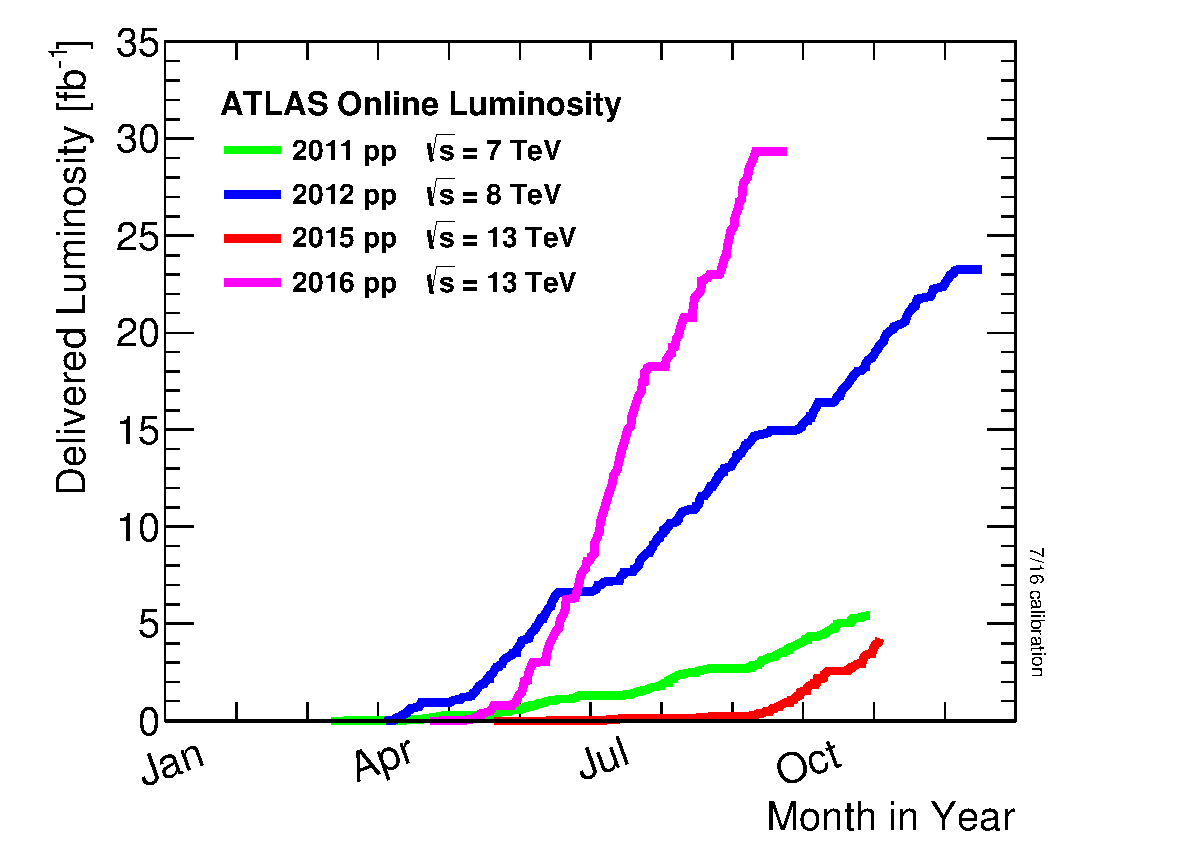
\includegraphics[width=\fullfig]{figures/lumi_years.pdf}
\caption{The cumulative luminosity over time delivered to the \ac{ATLAS} experiment from high energy proton-proton collisions since 2011. The energies of the collisions are listed for each of the data-taking periods.}
\label{fig:lumi_years}
\end{figure}

\section{Injection Chain}
The \ac{LHC} takes advantage of the presence of previously built accelerators at \ac{CERN} to work up to the target energy in consecutive stages.
The series of accelerators that feed into the \ac{LHC} are known collectively as the injection chain, and together with the \ac{LHC} form the accelerator complex.
The full complex is illustrated in Figure~\ref{fig:accelerator_complex}, which details the complex series required to reach collisions of 13 or 14 \TeV. 

\begin{figure}[h]
\centering
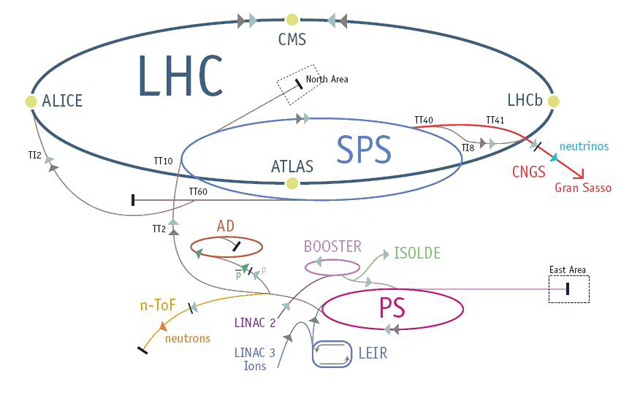
\includegraphics[width=\fullfig]{figures/accelerator_complex.jpg}
\caption{The accelerator complex that builds up to the full design energies at the \ac{LHC}. The protons are passed in order to Linac 2, the \acs{PSB}, the \acs{PS}, the \acs{SPS} and then the \ac{LHC}.}
\label{fig:accelerator_complex}
\end{figure}

Protons at the \ac{LHC} begin as hydrogen atoms in the Linac 2, a linear accelerator which replaced Linac 1 as the primary proton accelerator at CERN in 1978.
In Linac 2, the hydrogen atoms are stripped of their electrons by a strong magnetic field, and the resulting protons are accelerated up to 50 \MeV by cylindrical conductors charged by radio frequency cavities.
The protons are then transferred to the \ac{PSB}, which uses a stack of four synchrotron rings to accelerate the protons up to 1.4 \GeV.
Then the protons are injected into the \ac{PS} which again uses synchrotron rings to bring the energy up to 25 \GeV.
The intermediate step between Linac 2 and the \ac{PS} is not directly necessary, as the \ac{PS} can accelerate protons starting from as low as 50 \MeV.
The inclusion of the \ac{PSB} allows the \ac{PS} to accept a higher intensity of injection and so increases the deliverable luminosity in the \ac{LHC}.
The penultimate stage of acceleration is provided by the \ac{SPS}, a large synchrotron with a 7 km circumference that was commissioned at CERN in 1976.
During this step the protons increase in energy to 450 \GeV, after which they can be directly injected into the \ac{LHC}. 


The final step is the \ac{LHC} itself, which receives protons from the \ac{SPS} into two separate beam pipes which circulate in opposite directions.
The filling process at this steps takes approximately 4 minutes, and the subsequent acceleration to the final energy (6.5 \TeV during 2015 and up to 7 \TeV by design) takes approximately half an hour.
At this point the protons circulate around the circumference tens of thousands of times a second and continue for up to two hours.

% ----------------------------------------

\section{Design}

\subsection{Layout}

Many of the aspects of the \ac{LHC} design are driven by the use of the existing \ac{LEP} tunnel. 
This tunnel slopes gradually, with a 1.4\% decline, with 90\% of its length built into molasse rock which is particularly well suited to the application.
The circumference is composed of eight 2987 meter arcs and eight 528 meter straight sections which connect them; this configuration is illustrated in Figure~\ref{fig:lhc_schematic}.
The tunnel diameter is 3.7 m throughout its length. 

\begin{figure}
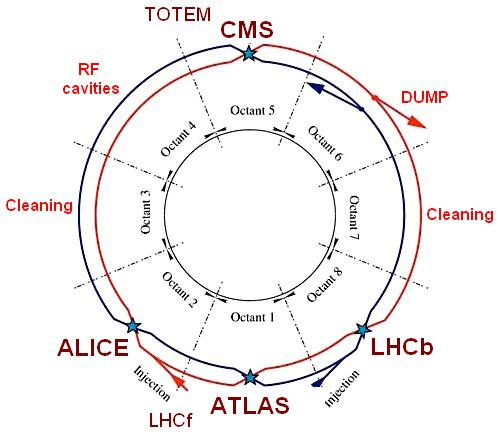
\includegraphics[width=\fullfig]{figures/lhc_schematic.jpg}
\caption{A schematic of the layout of the \ac{LHC}, not to scale. The arched and straight sections are illustrated at the bottom of the schematic, and all four crossing sites are indicated with their respective experiments.}
\label{fig:lhc_schematic}
\end{figure}

The design energy is directly limited by the size of this tunnel, with its radius of curvature of 2804 m. 
A significant magnetic field is required to curve the protons around that radius of curvature; the relationship is given by

\begin{align}
p \simeq 0.3BR \label{eq:magnetic_bending}
\end{align}

\noindent where p is the momentum of the particle in \GeV, B is the magnetic field in Tesla, and R is the radius of curvature in meters. 
From the target design energy of 14 \TeV, or 7 \TeV of momentum for protons in each beam, the required magnetic field is 8.33 Tesla.
This is too large a field strength to be practical with iron electromagnets, because of the enormous power required and the resulting requirements for cooling.
Because of these constraints, the \ac{LHC} uses superconducting magnets which can maintain that field strength with significantly less power consumption.

\subsection{Magnets}

The magnets chosen were Niobium and Titanium (NbTi) which allow for field strengths as high as 10 Tesla when cooled down to 1.9 K.
Reaching the target temperature of  1.9 K for all of the magnets requires superfluid helium and a large cryogenic system along the entire length of the tunnel.
During normal operation, the \ac{LHC} uses 120 tonnes of helium within the magnets, and the entire system is cooled by eight cryogenic helium refrigerators.
The temperature increase that occurs during transit from the refrigerator along the beam necessitates that the refrigerators cool the helium down to 1.8 K.
Any significant increase above this temperature range can remove the superconductive properties of the magnets, which in turn generates drastically larger heat losses from the current within the magnets and causes a rapid rise in temperature called a quench.

There are approximately 8000 superconducting magnets distributed around the \ac{LHC}.
The 1232 bending magnets, which keep the protons curving along the length of the beam, are twin bore cryodipoles, which allow both proton beams to be accommodated by one magnet and all of the associated cooling structure.
Figure~\ref{fig:dipole_magnet} shows the cross section of the design for these dipoles. 
The magnets are very large, 16.5 m long with a diameter of 0.57 meters and a total weight of 28 tonnes. 
They are slightly curved, with an angle of 5.1 mrad, in order to carefully match the beam path.
The twin bore accommodates both magnets inside the two 5 cm diameter holes which are surrounded by the superconducting coils.
The coils require 12 kA of current in order to produce the required magnetic field.
These coils are comprised of NbTi cable wound in two layers; the wire in the inner layer has a diameter of 1.065 mm while the wire in the outer layer has a diameter of 0.825 mm. 

\begin{figure}
\centering
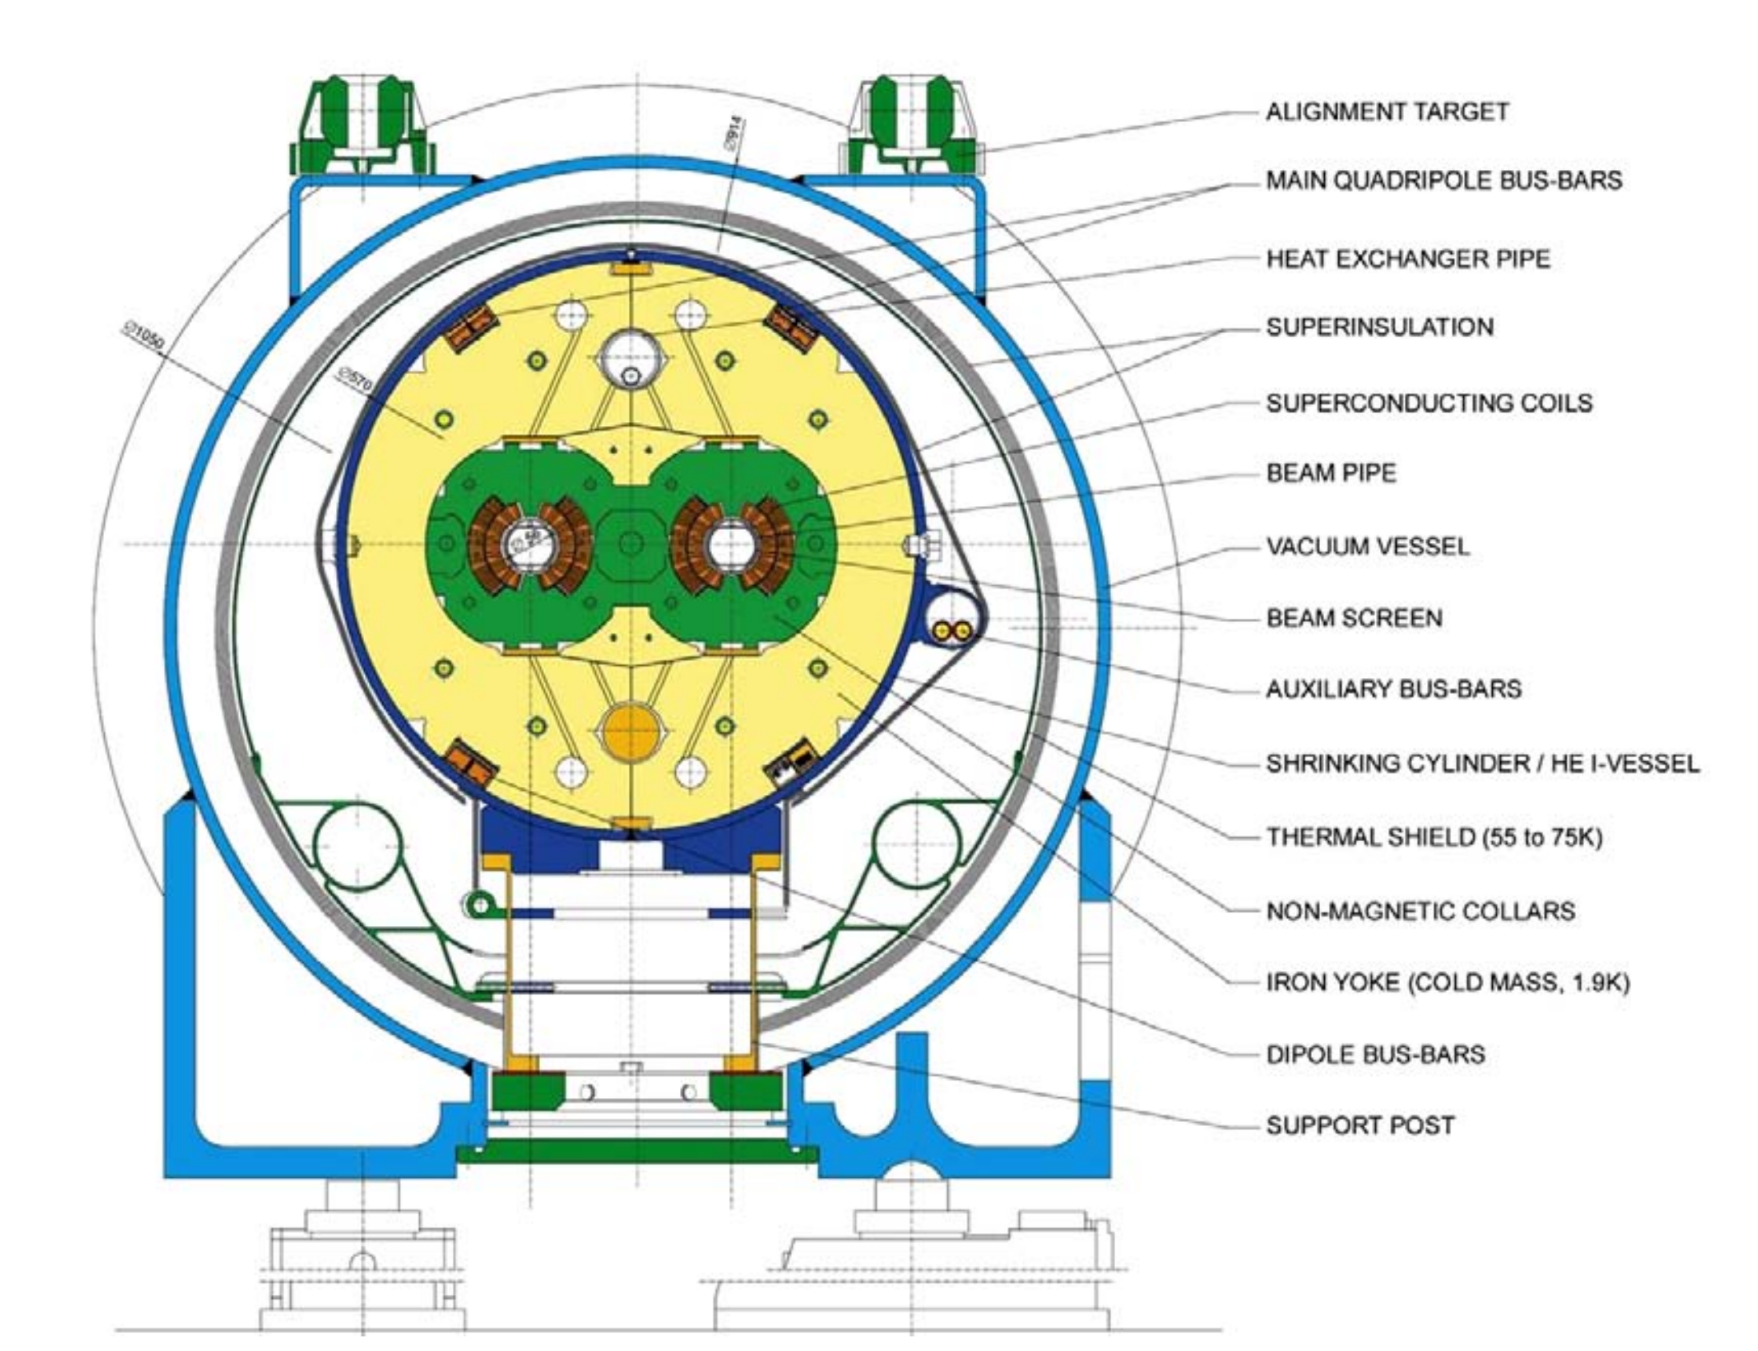
\includegraphics[width=\fullfig]{figures/dipole_magnet.png}
\caption{A cross section of the the cryodipole magnets which bend the flight path of protons around the circumference of the \ac{LHC}. The diagram includes both the superconducting coils which produce the magnetic field and the structural elements which keep the magnets precisely aligned.}
\label{fig:dipole_magnet}

\end{figure}

The large currents in the wires, along with the magnetic field produced, result in forces on the magnets which would tend to push them apart with over 10,000 Newtons per meter.
Constraining the magnets requires a significant amount of structure including non-magnetic stainless steel collars. 
Both the presence of these electromagnetic forces and the varying thermal contraction coefficient of the pieces of the magnet produce significant forces on the cold mass structure. 
The cold mass is carefully engineered to so that these stresses do not significantly alter the magnetic field shape, which must be maintained between magnets to a precision of approximately $10^{-4}$ for successful operation.

The remaining 6800 magnets are a variety of quadrupole, sextapole, octopole, and single bore dipole magnets.
These are used to damp oscillations, correct beam trajectories, focus the beams during circulation, and to squeeze the beams before collisions.

\subsection{\acs{RF} Cavities}
\label{sec:rfcavity}

Sixteen \ac{RF} cavities produce the  actual acceleration of the proton beam up to the design energy.
These \ac{RF} cavities are tuned to operate at 400 MHz, and are powered by high-powered electron beams modulated at the same frequency, called klystrons.
The resonance within the cavity with the oscillating electric field establishes a voltage differential of 2 MV per cavity.
The sixteen cavities are split between the two beams, so combined the cavities provide 16 MV per beam, which accelerate the protons on each consecutive pass through the cavity.
This acceleration is also necessary during circulation even after the target energy has been reach in order to compensate for losses from synchrotron radiation.

The cavities are arranged in cryomodules which contain four cavities, with two cryomodules per beam; this arrangement is illustrated in Figure~\ref{fig:rfcavity}.
These cryomodules are necessary to maintain the superconducting state of the cavities, which are also constructed from niobium.
The \ac{RF} cavities use niobium along with copper to allow for low power losses in the superconductors.
The copper provides a reduced susceptibility to quenching, as it rapidly conducts away heat generated by imperfections in the niobium, as well as natural shielding from the earth's magnetic field which can interfere with the \ac{RF} system.

\begin{figure}
\centering
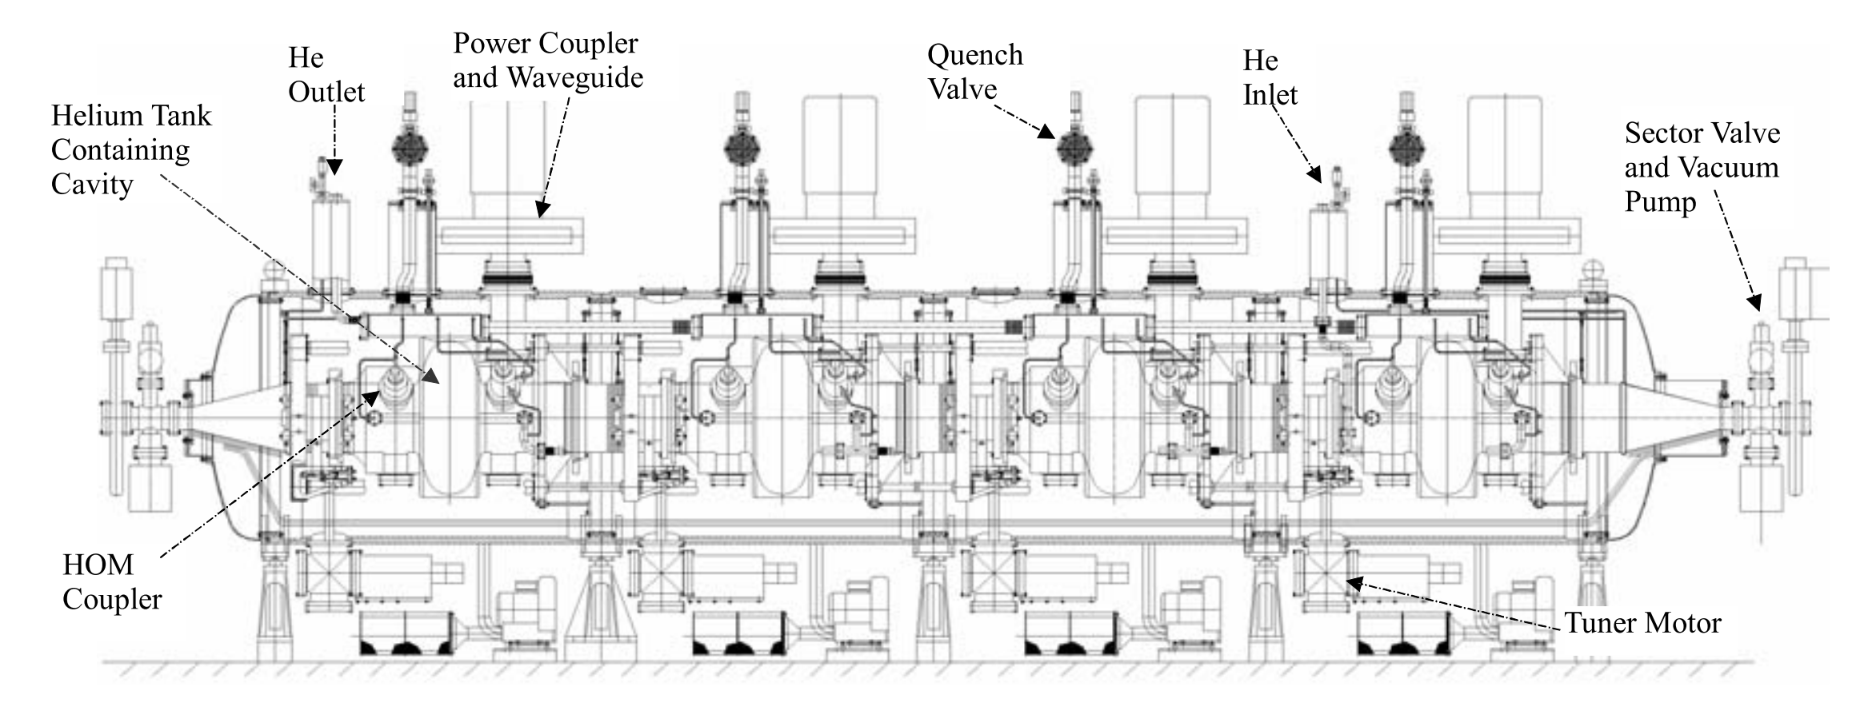
\includegraphics[width=\fullfig]{figures/rfcavity.png}
\caption{The arrangement of four \ac{RF} cavities within a cryomodule.}
\label{fig:rfcavity}
\end{figure}

The nature of the radio frequency oscillations tends to group protons together into buckets.
A proton traveling exactly in phase with the \ac{RF} oscillations will not be displaced at all during a single circulation, and those slightly ahead or behind of that phase will slightly decelerate or accelerate, respectively.
This produces separate clusters of protons which arrive in phase to the cavities every 2.5 ns, corresponding to the 400 MHz frequency.

\subsection{Beam}

The beams of protons circulate within 54 km of 5 cm diameter beam pipe.
This entire structure is kept under vacuum at 1.9 K to prevent interactions between the beam pipe and the magnets as well as to prevent any interactions between the circulating protons and gas in the pipe. 
The vacuum within the pipe establishes a pressure as low as 10\tsup{-9} mbar before the protons are introduced.

Because of the very high energies of the circulating protons, synchrotron radiation is not negligible in the bending regions.
The protons are expected to radiate 3.9 kW per beam at 14 \TeV, with 0.22 W/m, which is enough power to heat the liquid helium and cause a quench were it absorbed by the magnets.
To prevent this, a copper screen is placed within the vacuum tube that absorb the emitted photons.
This screen is kept between 5 and 20 K by the liquid helium cooling system.

% ----------------------------------------

\section{Luminosity Parameters}

In addition to the high energy of the collisions, the rate of collisions is extremely important to enabling the discovery of new physics.
Many measurements and searches require a large number of events in order to be able to make statistically significant conclusions.
The rate of collisions is measured using luminosity, the number of collisions per unit time and unit cross section for the proton-proton collisions.
From the beam parameters, luminosity is given by 

\begin{align}
\mathcal{L} = \frac{N_b^2 n_b f_{rev} \gamma}{4\pi \epsilon_n \beta^*} F \label{eq:luminosity} 
\end{align}

\noindent where $N_b$ is the number of protons per bunch, $n_b$ is the number of bunches per beam, $f_{rev}$ is the frequency of revolution, $\gamma$ is the Lorentz factor for the protons at the circulating energy, $\epsilon_n$ is the emittance, $\beta^*$ is the amplitude function at the collision point, and F is a geometric factor that accounts for the crossing angle of the beams at the collision point. 
The emittance measures the average spread of particles in both position and momentum space, while the amplitude function is a beam parameter which measures how much the beam has been squeezed. 
Together $\epsilon_n$ and $\beta^*$ give the size of the beam in the transverse direction, $\sigma = \sqrt{\epsilon\beta^*}$. 
$\beta$ changes over the length of the beam as the accessory magnets shape the distribution of protons, but only the value at the point of collisions, $\beta^*$, affects the luminosity.

The luminosity is maximized to the extent possible by tuning the parameters in Equation~\ref{eq:luminosity}.
A number of these are constrained by the design decisions.
The revolution frequency is determined entirely by the length of the tunnel, as the protons travel at very close to the speed of light.
The geometric factor F is determined by the crossing angle of the beams at the collision points, again a component of the tunnel design; this angle is already very small at 285 $\mu$rad, which helps to maximize the geometric factor.

The major pieces that can be adjusted are the number of protons per bunch, $N_b$, the number of bunches in the beam, $n_b$, and the amplitude function $\beta$.
Increasing either $N_b$ or $n_b$ increases the amount of energy stored in the beam, which presents a danger if control of the beam is lost.
At design specifications, the beam stores 362 MJ, which is enough energy to damage the detectors or accelerator if the beam were to wander out of the beam pipe.
So, the luminosity is primarily controlled at the \ac{LHC} by adjusting $\beta^*$, where lowering $\beta^*$ increases the luminosity.
$\beta^*$ is tuned to provide the various values of luminosity used at the \ac{LHC} which can be raised to as much as 10\tsup{34}.

The nominal bunch structure consists of 3654 bunches, each holding 10\tsup{11} protons, which cross a collision point in 25 ns. 
These are further subdivided into the buckets mentioned in Section~\ref{sec:rfcavity} by the clustering properties of the \ac{RF} cavities.
The bunches are further grouped into trains of 72 bunches which are separated by a gap which would otherwise hold 12 bunches.
At nominal operation 2808 of the bunches will actually be filled with protons, while the remainder are left empty to form an abort gap that can be used in case the beam needs to be dumped.

The various beam parameters are summarized in Table~\ref{tab:beam_parameters} for the designed operation.
In practice, the beam has operated at lower energies and lower luminosities than the design values for the majority of its lifetime, but the \ac{LHC} has begun to operate at full design values during Run 2.

\begin{table}
\begin{tabular}{lccc}
\hline
Parameter & Unit & Injection & Nominal \\
\hline
Beam Energy & \TeV & 0.450 & 7 \\
Peak Instantaneous Luminosity & \lcms & - & 10\tsup{34} \\
Bunch Spacing & ns & 25 & 25 \\
Number of Filled Bunches & - & 2808 & 2808 \\
Normalized Transverse Emittance & $\mu$m & 3.75 & 3.75 \\
Frequency & MHz &  400.789 & 400.790 \\
RF Voltage/Beam & MV & 8 & 16 \\
Stored Energy & MJ & - & 362 \\
Magnetic Field & T & 0.54 & 8.33 \\
Operating Temperature & K & 1.9 & 1.9 \\
\hline
\end{tabular}
\caption{The design parameters of the \ac{LHC} beam that determines the energy of collisions and the luminosity, for both the injection of protons and at the nominal circulation.}
\label{tab:beam_parameters}
\end{table}


% ----------------------------------------

\section{Delivered Luminosity}

During the data collection of 2015, the \ac{LHC} operated at luminosities as larges as 5 $\times$ 10\tsup{33} \lcms.
It is convenient to refer to the integrated luminosity, the integral of the instantaneous luminosity, which corresponds directly to the number of delivered events for a given process.
\[ N = \sigma \times \int \mathcal{L}(t)dt \]
where $\sigma$ is the cross section for the process of interest.
The integrated luminosity over time is shown in Figure~\ref{fig:lumi_2015}.
This includes the luminosity delivered by the \ac{LHC} as well as the luminosity that was recorded by \ac{ATLAS}.
\ac{ATLAS} only records collisions when the \ac{LHC} reports that the beam conditions are stable, so some of the delivered luminosity is not recorded.
The figure also includes the amount of luminosity marked as good for physics, which includes additional requirements on the operation of the detector during data collection that are necessary for precise measurements. 


\begin{figure}
\centering
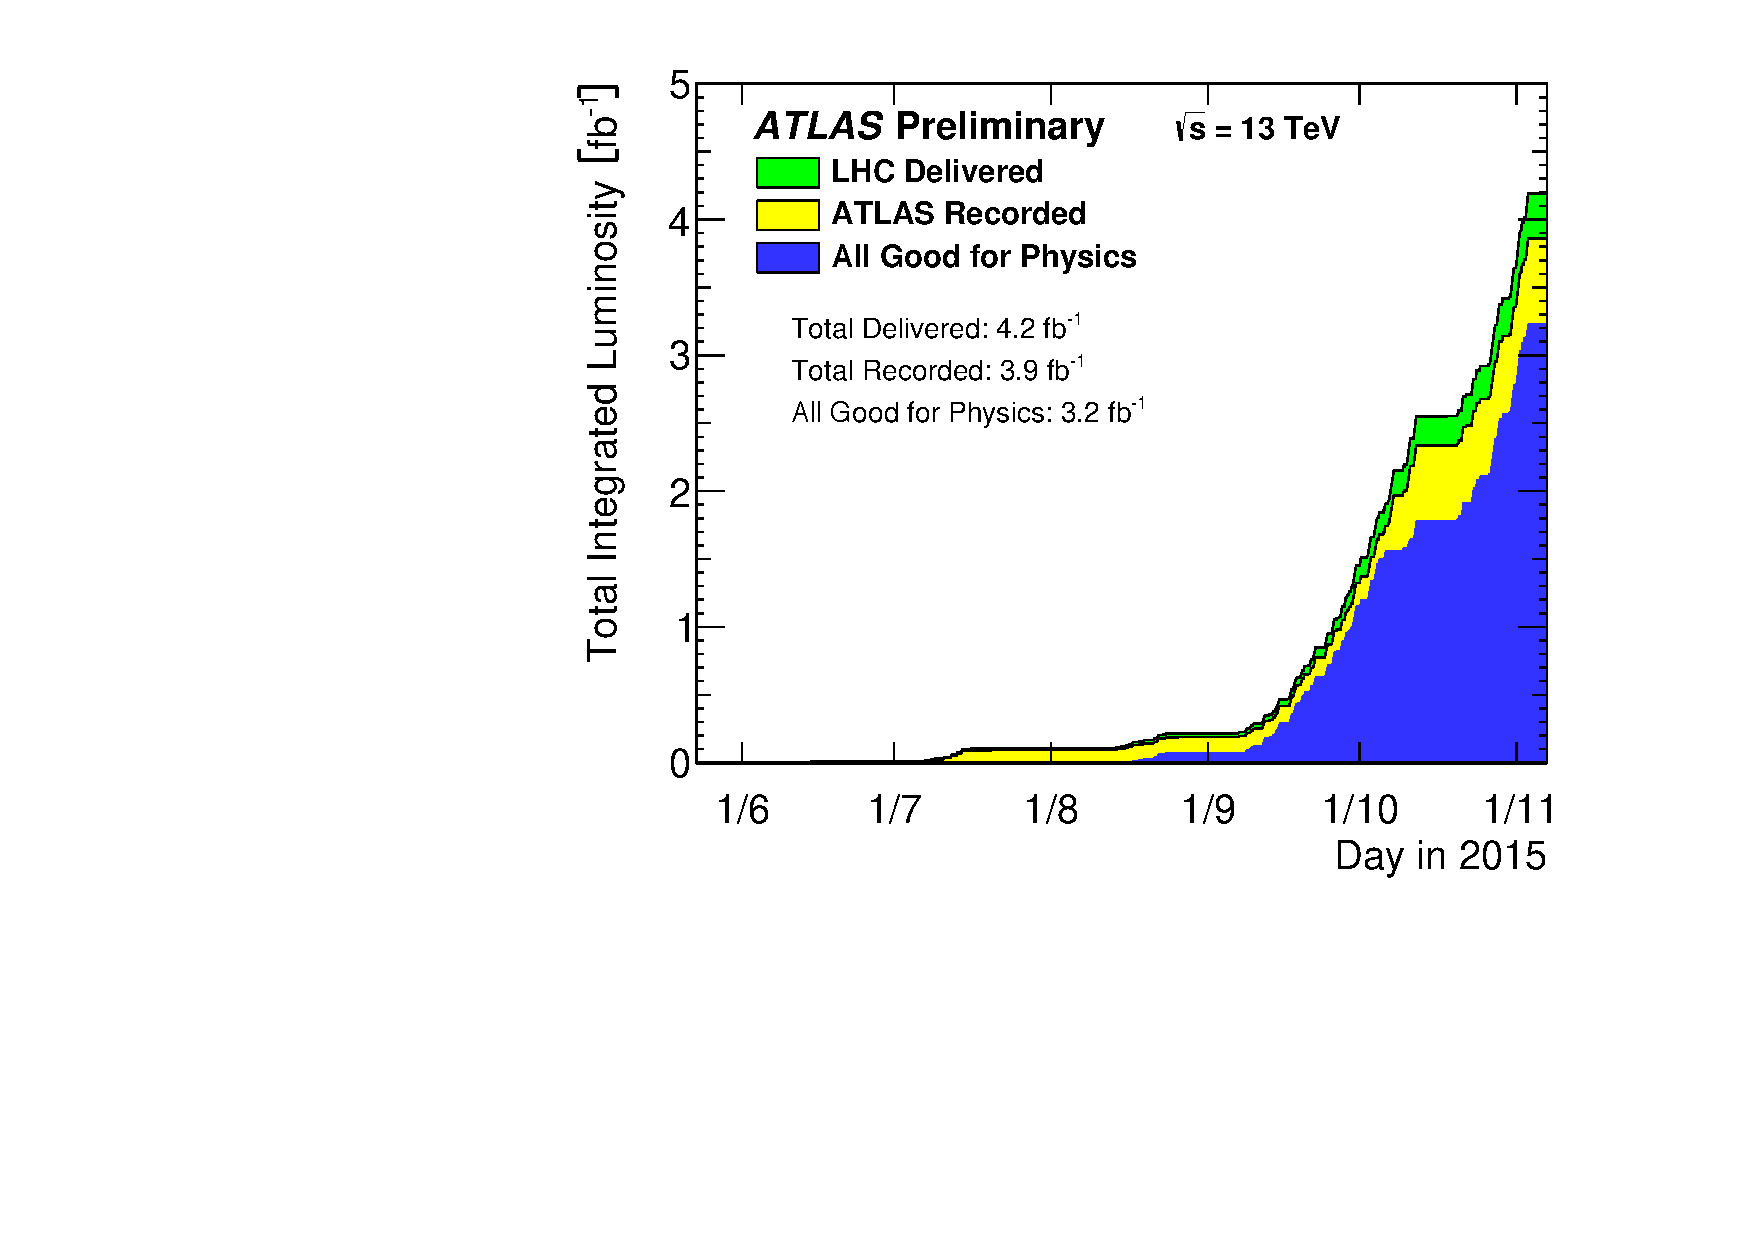
\includegraphics[width=\fullfig]{figures/lumi_2015.pdf}
\caption{The cumulative luminosity versus time delivered to ATLAS (green), recorded by ATLAS (yellow), and certified to be good quality data (blue) during stable beams for pp collisions at 13 \TeV in 2015.}
\label{fig:lumi_2015}
\end{figure}

Because the beam circulates and collides bunches of protons, it is possible for a single crossing to produce multiple proton-proton collisions.
As the instantaneous luminosity is increased, the average number of collisions generated per bunch crossing increases.
An event refers to the entire collection of interactions during a single bunch crossing, while interactions refer to the individual proton-proton collisions.
The additional interactions produced during each bunch crossing are referred to as pileup, which can be more precisely defined quantified using the average number of additional proto-proton interactions per corrsing, often denoted $\mu$.
Figure~\ref{fig:mu_2015} shows the luminosity-weighted distribution of the mean number of interactions for events collected in 2015.
The presence of as many as twenty interactions in a single collision provides a significant challenge in reconstructing events and isolating the targeted physical processes. 

\begin{figure}
\centering
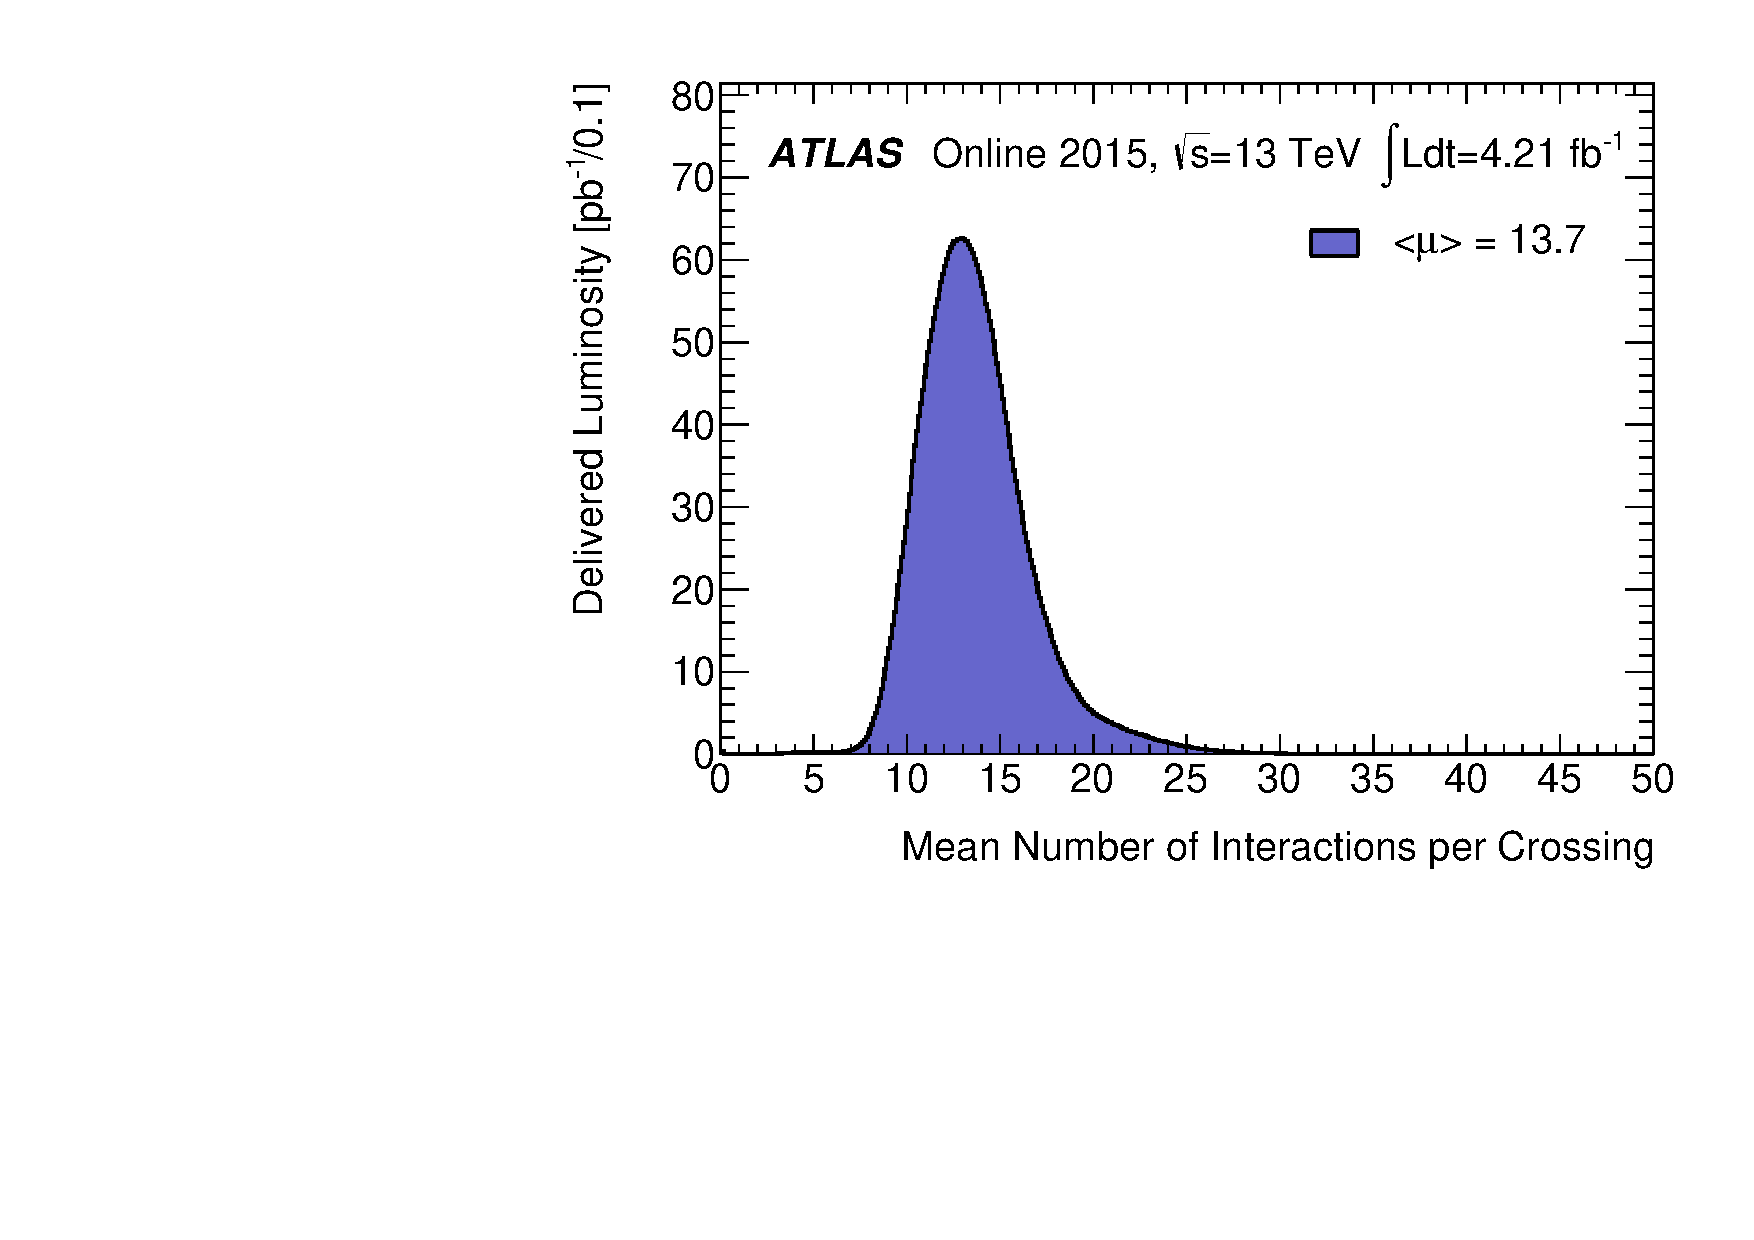
\includegraphics[width=\fullfig]{figures/mu_2015.pdf}
\caption{The luminosity-weighted distribution of the mean number of interactions per crossing for the 2015 pp collision data at 13 \TeV.}
\label{fig:mu_2015}
\end{figure}

\chapter{The ATLAS Detector}

\label{ch:atlas}
% --------------------------------------------------------------------------------

The four major \ac{LHC} experiments at \ac{CERN} seek to use the never before matched energies and luminosities of the new collider to explore the boundaries of particle physics and to gain insight into the fundamental forces of nature.
Two of these experiments, ATLAS and \ac{CMS}, are general purpose detectors that seek to measure a variety of processes in the up to 13 \TeV proton-proton collisions that occur as much as 800 million times per second at the \ac{LHC} at the design luminosity of $10^{34}$ \lcms. 
ATLAS employs a hermetic detector design, one which encloses the particle collisions as completely as possible with detecting elements, that allows it to study a wide range of physics from \ac{SM} precision measurements to searches for new physics in models like \ac{SUSY}~\cite{atlas_experiment}.

Accommodating this wide variety of goals is a challenge for the design of the detector.
The wide range of energies involved requires high measurement precision over several orders of magnitude, and the numerous physics processes require an ability to measure a variety of particle types.
At the time of the construction of ATLAS, the Higgs boson had yet to be discovered, but the diphoton decay mode was (correctly) expected to be important and necessitated a high resolution photon measurement.
The potential for decays of new heavy gauge bosons, W' and Z', required a similarly high momentum resolution for leptons with momentum up to several \TeV.
Hadronic decay modes of several possible new high energy particles could result in very energetic jets, again up to several \TeV, and reconstructing the decay resonances would again require good energy resolution.
Several models, such as \ac{SUSY} or Extra Dimensions, predict the existence of particles which would not interact with traditional detecting elements. 
However these particles can still be observed in a hermetic detector by accurately measuring the remaining event constituents to observe an imbalance in energy called missing energy or \met. 
Measuring \met implicitly requires a good resolution on all \ac{SM} particles that can be produced.
And at the lower end of the energy spectrum, precision \ac{SM} measurements would require good resolution of a variety of particle types at energies as low as a few \GeV, so the design needs to accommodate roughly three orders of magnitude.

This broad spectrum of measurements requires a variety of detector systems working together to form a cohesive picture of each collision. 
Two large magnet systems produce magnetic fields that provide a curvature to the propagation of charged particles and allows for precision momentum measurements in the subdetectors.
The inner detector uses a combination of detector technologies to reconstruct particle trajectories and vertices for charged particles.
A variety of calorimeters measure the energies of hadrons, electrons, and photons over a large solid angle.
A large muon spectrometer identifies muons and uses the second magnet system to provide an independent measurement of their momentum from the inner detector and improve the resolution. 
The layout of all of these systems is shown in Figure~\ref{fig:atlas_overview}.

% Particle interaction summaries should go somewhere, maybe at the end? Come back to this to figure out where fig:particle_slice should go.

The performance goals needed to achieve the various targeted measurements and searches discussed above can be summarized as resolution and coverage requirements on each of these systems.
Those requirements are listed in Table~\ref{tab:performance_goals}.

\begin{figure}[hbtp]
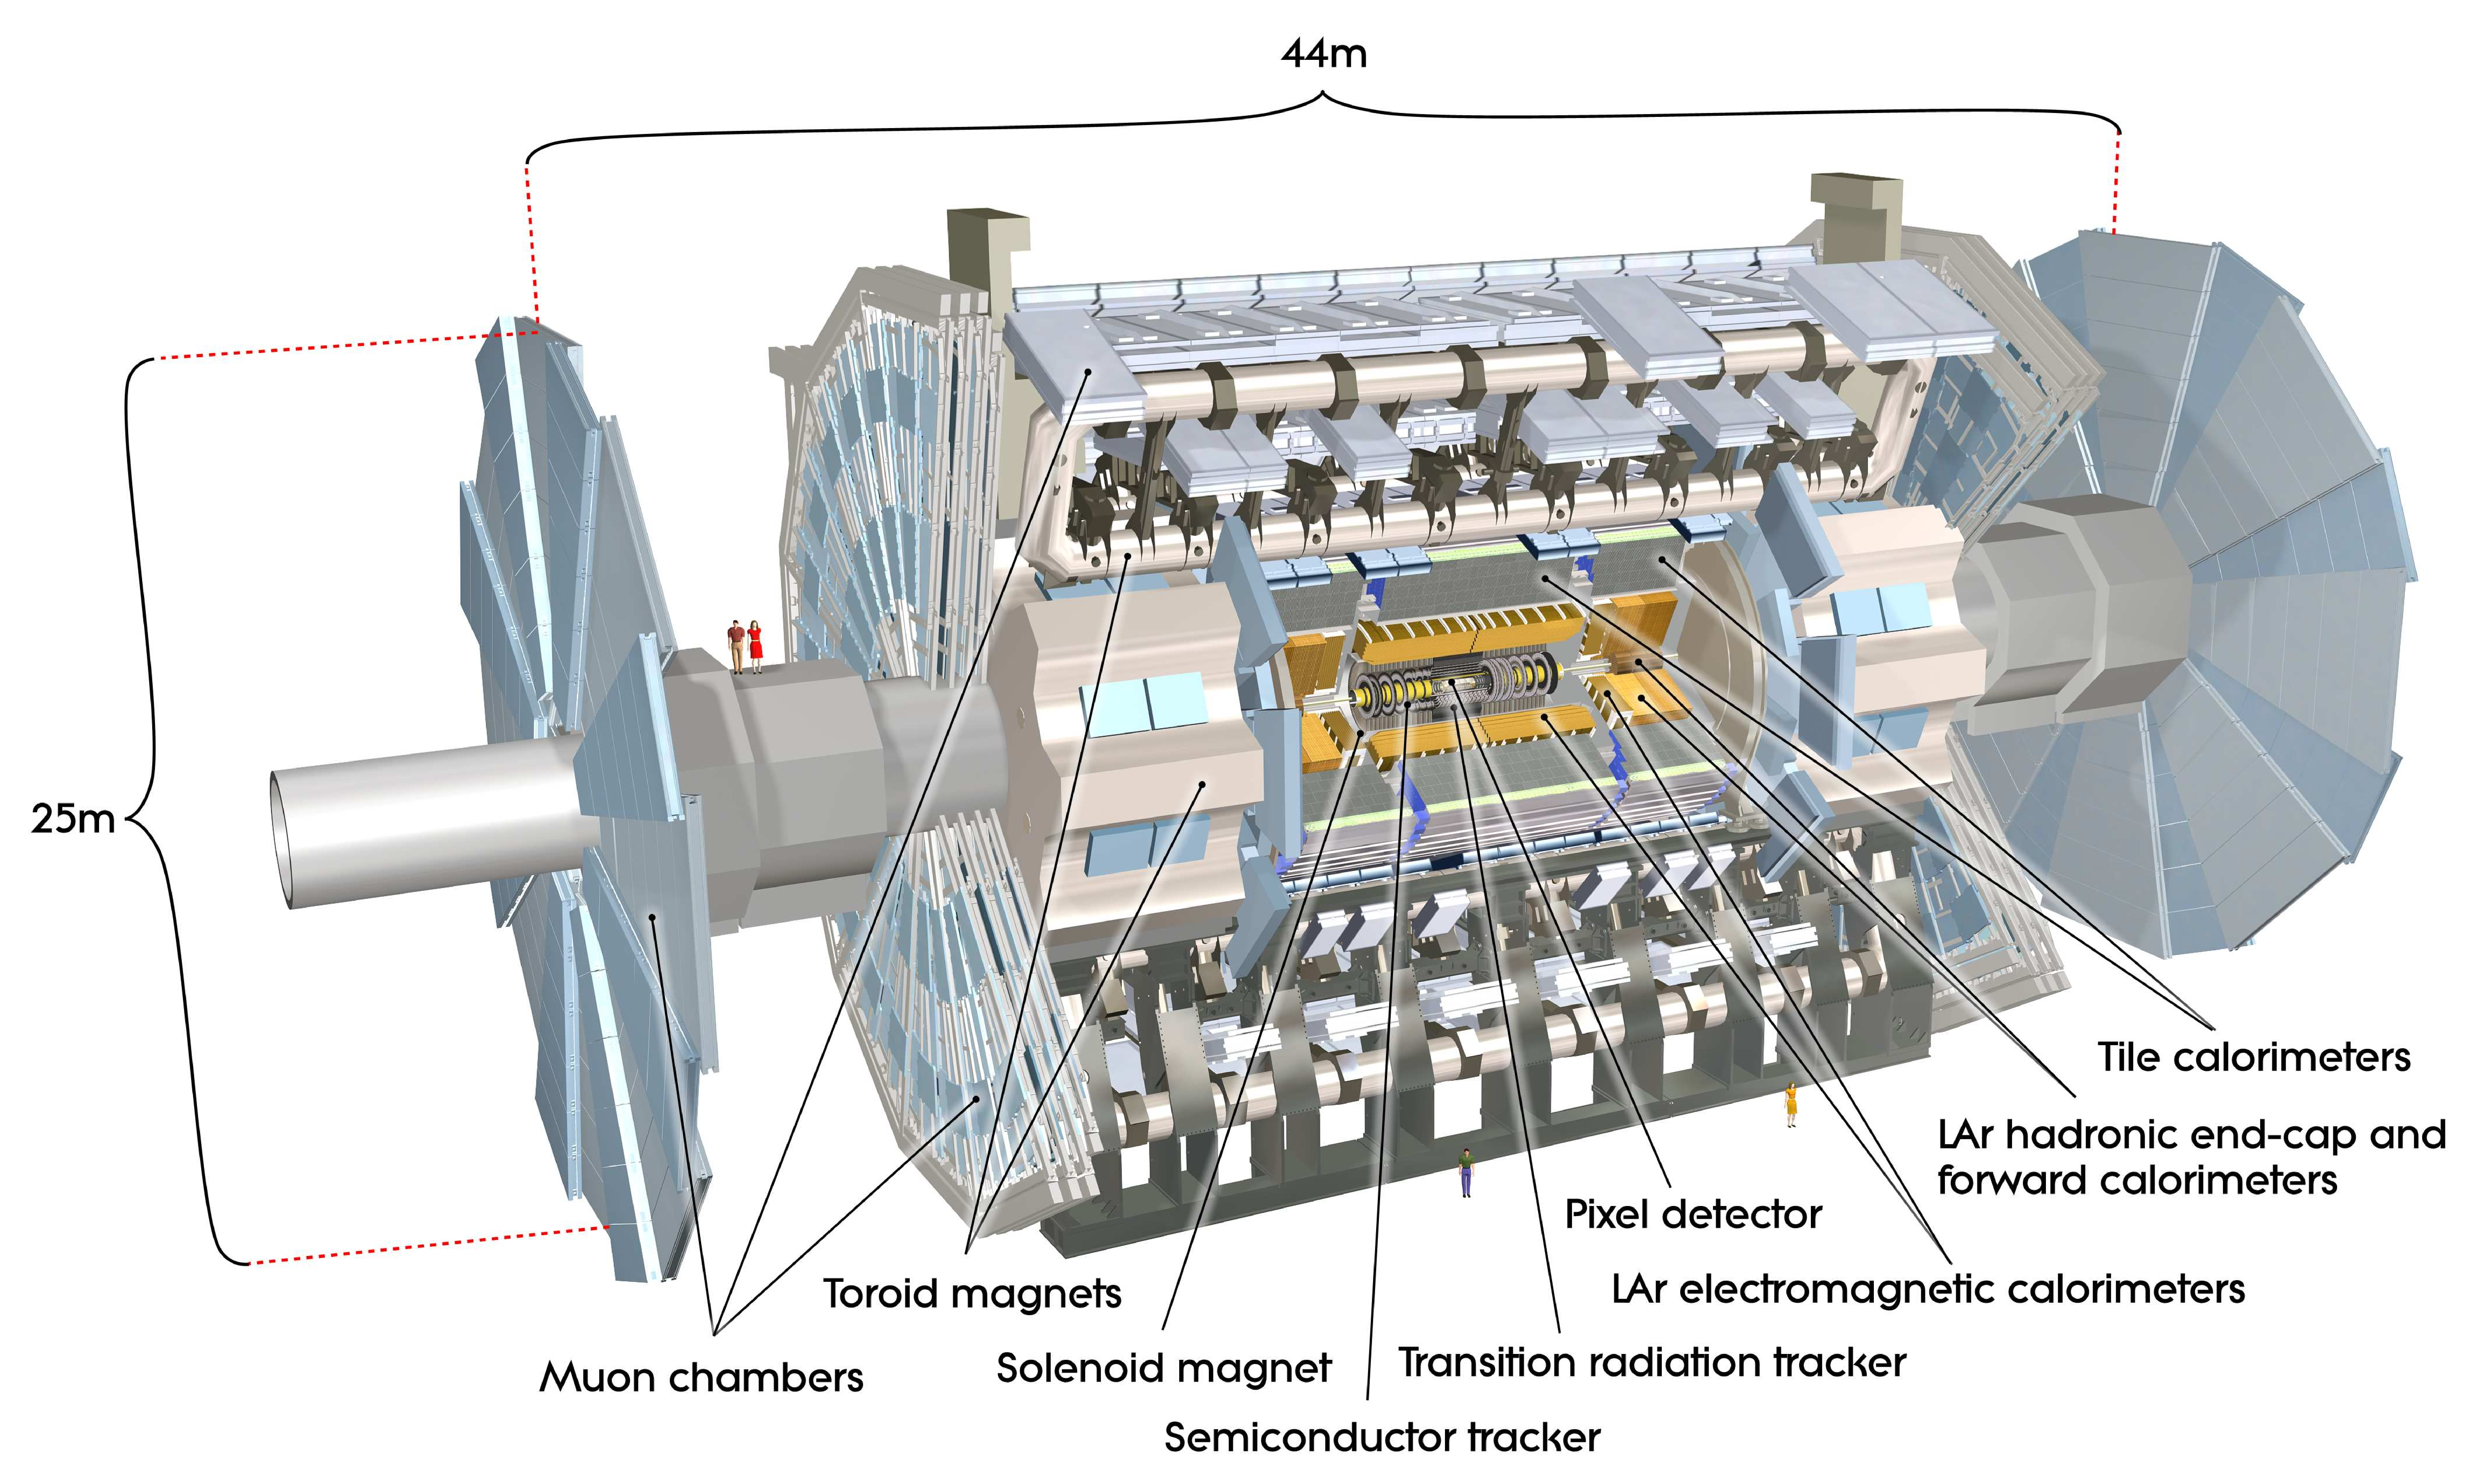
\includegraphics[width=\fullfig]{figures/atlas_overview.pdf}
\caption{A cut-away schematic of the layout of the ATLAS detector. Each of the major subsystems is indicated.}
\label{fig:atlas_overview}
\end{figure}

\begin{figure}[hbtp]
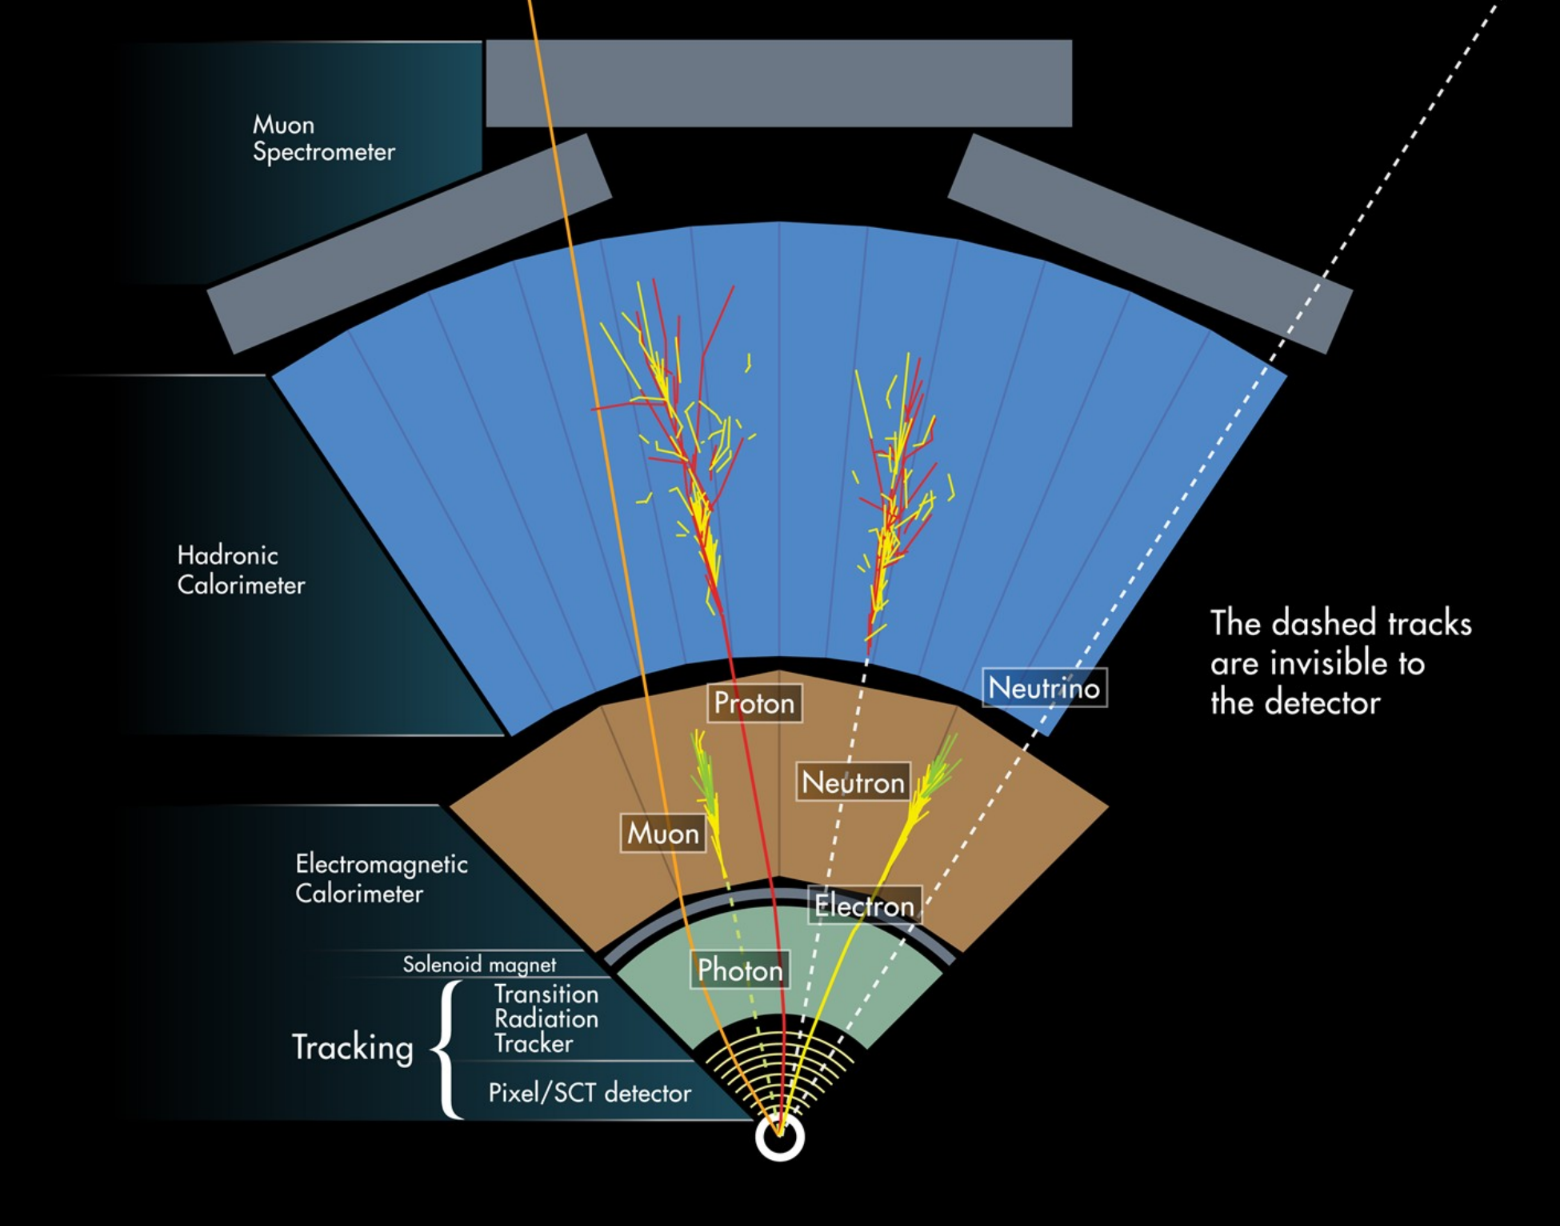
\includegraphics[width=\fullfig]{figures/particle_interactions.png}
\caption{A cross-sectional slice of the ATLAS experiment which illustrates how the various \ac{SM} particles interact with the detector systems.}
\label{fig:particle_interactions}
\end{figure}

\begin{table}
\centering
\begin{tabular}{llcc}
  \hline
  Detector Component & Required Resolution & \multicolumn{2}{c}{$|\eta|$ Coverage} \\
                     &                     & Measurement & Trigger \\
  \hline
  Tracking & $\sigma_{\pt}/\pt = 0.05\% \pt \oplus 1\%$ & $2.5$ & - \\
  EM Calorimetry & $\sigma_{E}/E = 10\%/\sqrt{E} \oplus 0.7\%$ & $3.2$ & $2.5$ \\
  Hadronic Calorimetry & & \\
  \quad Barrel and Endcap & $\sigma_{E}/E = 50\%/\sqrt{E} \oplus 3\%$ & $3.2$ & $3.2$ \\
  \quad Forward & $\sigma_{E}/E = 100\%/\sqrt{E} \oplus 10\%$ & $3.1 - 4.9$ & $3.1 - 4.9$ \\
  Muon Spectrometer & $\sigma_{\pt}/\pt \leq 10\%$ for $p_T \leq 1\ \TeV$ & $2.7$ & $2.4$ \\
  \hline
\end{tabular}
\caption{The performance goals for each of the subsystems of the ATLAS detector. The $|\eta|$ coverage specifies the range where the subsystem needs to be able to provide measurements with the specified resolution. The resolutions include a \pt or E dependence that is added in quadrature with a \pt/E independent piece.}
\label{tab:performance_goals}
\end{table}

Incorporating these various pieces into a single detector is a significant technical challenge.
The resulting detector has a diameter of 22 m, is 46 m long, and weighs 7,000 tons; it is the largest volume particle detector ever constructed.
The various detector elements need to be constructed and assembled with precision as low as micrometers.
These systems all need to function well even after exposure to the significant radiation dose from the collisions.
Designing, constructing, and installing the detector took the combined effort of more than 3000 scientists from 38 countries over almost two decades.


\section{Coordinate System}

The coordinate system defined for the ATLAS detector is used throughout all of the sections of this thesis.
The system begins with the choice of a $z$ axis along the beamline.
The positive $z$ side of the detector is commonly referred to as the $A$-side, and the negative $z$ side is referred to as the $C$-side.
The $x-y$ plane is then the plane transverse to the beam direction, with the $x$ direction defined as pointing from the interaction point to the center of the \ac{LHC} ring and the $y$ direction defined as pointing upwards.
The nominal interaction point is the origin of this system.

It is more convenient in practice to use a cylindrical coordinate system; this choice of coordinate system reflects the cylindrical symmetry of the ATLAS detector.
The distance from the beamline is the radius, $r$', and the angle from the $z$-axis is $\theta$.
The azimuthal angle, $\phi$, runs around the $z$-axis with $\phi = 0$ corresponding to the $x$-axis.
Many aspects of the detector are independent of this coordinate to first order; the detector is symmetric in $\phi$.
The $\theta$ direction is typically specified using rapidity or pseudorapidity, where rapidity is defined as

\begin{equation}\label{eq:rapidity}
y = \frac{1}{2} \ln \frac{E + p_z}{E - p_z}
\end{equation}

\noindent Rapidity is particularly useful to indicate the component along the $z$ direction because differences in rapidity are invariant to boosts along the $z$-direction.
A similar quantity which depends only the $\theta$ is the pseudorapidity, 

\begin{equation}\label{eq:pseudorapidity}
\eta = - \ln \tan \frac{\theta}{2}
\end{equation}

\noindent which approaches rapidity in the limit where the energy is much larger than the particle's mass and is identical for massless particles.
It is often useful to refer to differences in solid angle using the pseudorapidity and the azimuthal angle:

\begin{equation}\label{eq:deltar}
\Delta R = \sqrt{\Delta \phi^2 + \Delta \eta^2}
\end{equation}


The pseudorapidity is also invariant to boosts along the $z$-axis for high momentum particles, and is preferable to rapidity because it does not depend on the specific choice of particle.
Pseudorapidity is also preferable to $\theta$ because particle production is roughly uniform in equal-width intervals of $\eta$ up to about $\eta = 5.0$. 
A particle traveling along the beampipe has $\eta = \infty$ and a particle traveling perpendicular to the beampipe has $\eta = 0$.
The extent of the tracker, $|\eta| < 2.5$, corresponds to approximately $0.05 \pi < \theta [\mathrm{rad}] < 0.95 \pi$ and the extent of the calorimeters, $|\eta| < 4.9$ corresponds to approximately $0.005 \pi < \theta [\mathrm{rad}] < 0.995 \pi$.
Many detector components are broken into multiple subsystems to provide coverage at greater $|\eta|$.
The lower $|\eta|$ region is referred to as the barrel, typically with $|\eta| \lesssim 1.4$, and the greater $|\eta|$ region is often referred to as the endcap.

The initial momentum along the $z$ direction of the constituents in a proton-proton collision is unknown in hadron colliders because the constituent momenta vary between collisions (Section~\ref{sec:ppcollisions}).
Along the transverse plane, however, the vector sum of momentum will be zero.
For this reason, many physical quantities are quantified in terms of their projection onto the transverse plan, such as \pt or $E_T$.
In addition, \pt alone determines the amount of curvature in the magnetic field, and can be measured independently by measuring the curvature of a particle's propagation.


\section{Magnetic Field}
\label{sec:magnetic_field}

The magnet system used in ATLAS is designed to provide a substantial magnetic field in the two regions where the trajectory of particles is measured, the inner detector and the muon spectrometer.
The magnetic field generates a Lorentz force that curves the trajectory of charged particles, following Equation~\ref{eq:magnetic_bending}.
This allows the precision tracking elements to make high resolutions measurements of \pt.
To provide a magnetic field in these regions, ATLAS uses a hybrid system with four separate, superconducting magnets.
A single solenoid provides a 2 T axial, uniform magnetic field for the inner detector, while a barrel toroid and two endcap toroids produce a non-uniform magnetic field of 0.5 and 1 T, respectively, for the muon detectors.
This geometry is illustrated in Figure~\ref{fig:magnets_overview}, and the parameters of the three magnet systems are summarized in Table~\ref{tab:magnet_parameters}.

\begin{figure}[hbtp]
\centering
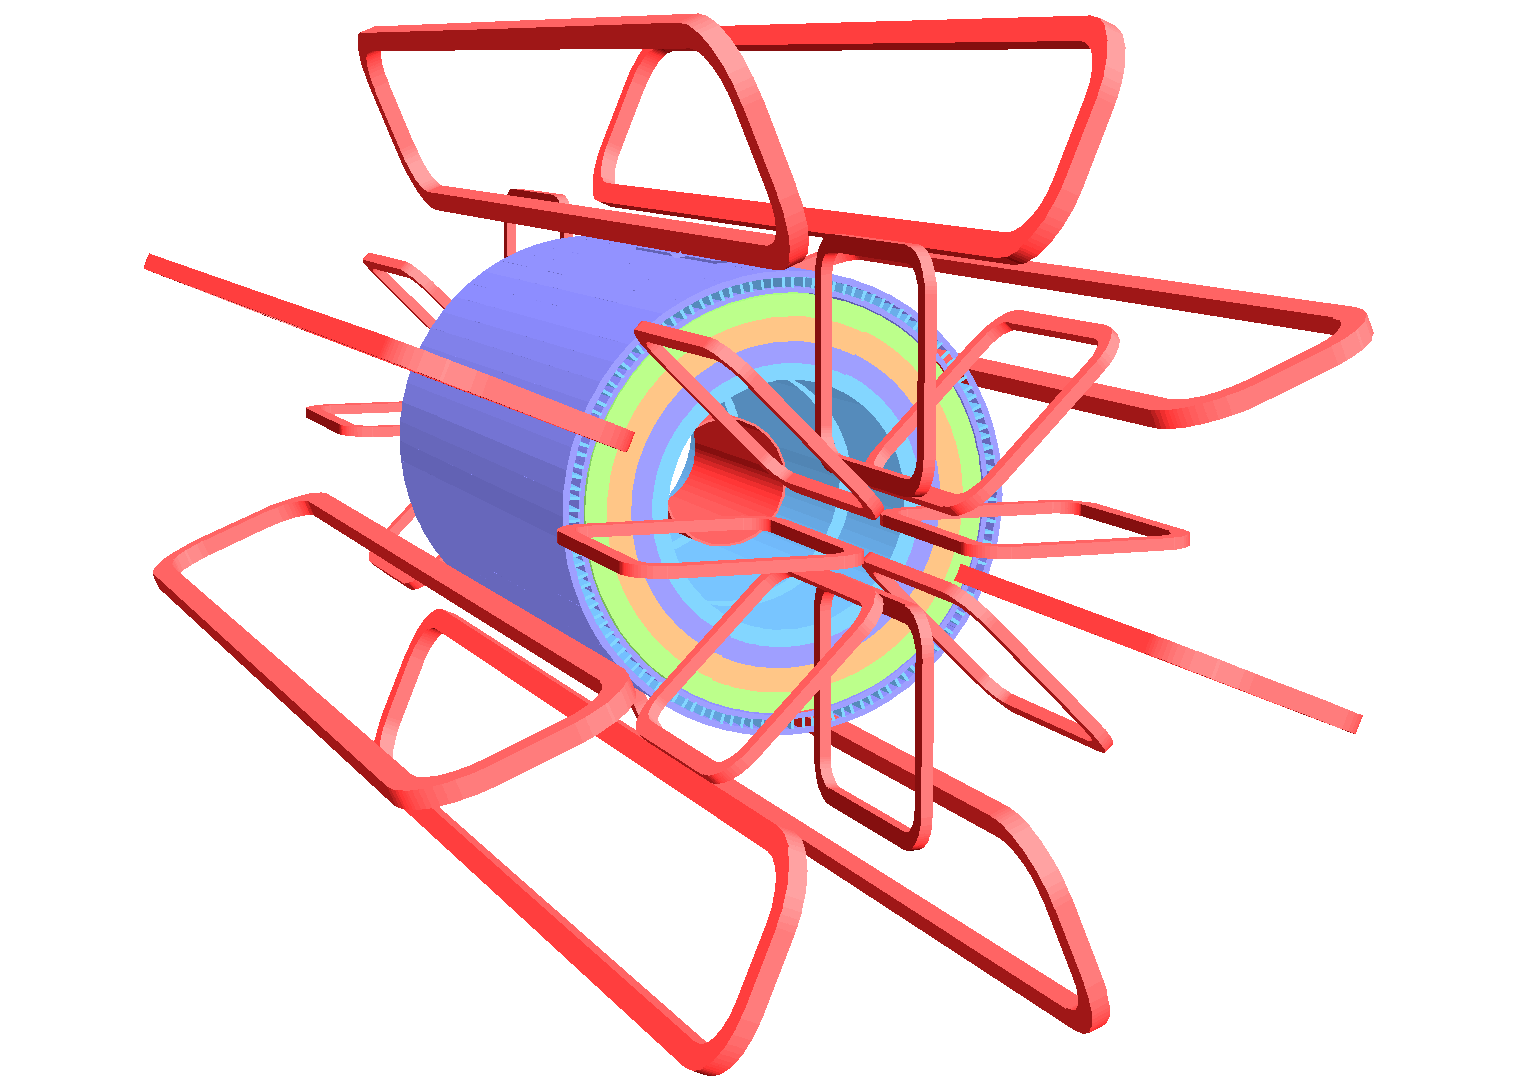
\includegraphics[width=\fullfig]{figures/magnets_overview.pdf}
\caption{The layout of the four superconducting magnets in the ATLAS detector.}
\label{fig:magnets_overview}
\end{figure}

\begin{table}
\centering
\begin{tabular}{lcccc}
\hline
Parameter & Unit & Solenoid & Barrel Toroid & Endcap Toroids \\
\hline
Inner Diameter & m & 2.4 & 9.4 & 1.7 \\
Outer Diameter & m & 2.6 & 20.1 & 10.7 \\
Axial Length & m & 5.3 & 25.3 & 5.0 \\
Weight & tons & 5.7 & 830 & 239 \\
Conductor Size & mm\tsup{2} & 30$\times$4.25 & 57$\times$12 & 41$\times$4.25 \\
Peak Field & T & 2.6 & 3.9 & 4.1\\
Heat Load & W & 130 & 990 & 330 \\
Current & kA & 7.7 & 20.5 & 20.0 \\
Stored Energy & MJ & 38 & 1080 & 206 \\
\hline
\end{tabular}
\caption{A summary of the parameters of each of the three magnet systems on ATLAS.}
\label{tab:magnet_parameters}
\end{table}

The central solenoid uses a single-layer coil with a current of 7.730 kA to generate the 2 T axial field at the center of the magnet. 
The single-layer coil design enables a minimal amount of material to be used in the solenoid's construction, which is important because the solenoid is placed between the inner detector and the calorimeters.
At normal incidence the magnet has only 0.66 radiation lengths worth of material, where one radiation length is the mean distance over which a high-energy electron loses all but $1/e$ of its energy through material interactions~\cite{pdg}.
The coil is made of a high-strength aluminum stabilized NbTi superconductor which was optimized to achieve a high field with minimal thickness.
The axial magnetic field produced by the solenoid bends charged particles in the $\phi$ direction, following a circular path with a radius specified by Maxwell's equations (see Equation~\ref{eq:magnetic_bending}). 

The barrel toroid consists of eight coils which generate a 0.5 T magnetic field, on average, in the cylindrical region around the calorimeters with an approximately 20 kA current.
The coils are separated only by air to reduce the scattering of muons as they propagate through the region.
The coils are made of an aluminum stabilized NbTiCu superconductor and each is separately housed in a vacuum and cold chamber.
This magnetic configuration produces a field in the $\phi$ and so curves muons traversing the volume primarily in the $\eta$ direction.

The endcap toroids follow a similar design to the barrel toroid and produce a 1.0 T magnetic field, on average. 
Each has eight separate NbTiCu coils, and in this case all eight are housed within a single cold mass.
This extra structure is necessary to withstand the Lorentz forces exerted by the magnets. 
These magnets are rotated 22.5\% relative to the barrel toroid to provide a uniform field in the transition between the two systems. 
The endcap toroids also produce a field in the $\phi$ direction and curve muons primarily in the $\eta$ direction.

% ----------------------------------------

\section{Inner Detector}
\label{sec:inner_detector}

The ATLAS inner detector provides excellent momentum resolution as well as accurate primary and secondary vertex measurements through robust pattern recognition that identifies tracks left by charged particles. 
These tracks fulfill a number of important roles in the ATLAS measurement system: they measure the momentum of charged particles including electrons and muons, they can identify electrons, they assign particles to different vertices, and they provide a correction to \met measurements from low energy particles. 
The system has to be accurate enough to separate tracks from dozens of vertices, to resolve each vertex individually, and to measure the \pt of very high momentum tracks which curve very little even in the large magnetic field.
This is accomplished by several independent layers of tracking systems.
Closest to the interaction point is the very high granularity Pixel detector, including the newly added \ac{IBL}, which is followed by the \ac{SCT} layers.
These silicon subdetectors both use discrete space-points to reconstruct track patterns.
The final layer, the \ac{TRT}, uses many layers of straw tube elements interleaved with transition radiation material to provide continuous hits in the transverse plane.
%The arrangement of these subdetectors is shown in Figure~\ref{fig:id_overview}.
To provide the desired hermetic coverage, the subdetectors are divided into barrel and endcap geometries.
Figure~\ref{fig:id_detail_schematic} shows the layout of the subdetectors in more detail, and illustrates how tracks at various pseudorapidities can traverse the subdetectors; tracks with $\eta > 1.1$ begin to traverse the endcap subdetectors rather than those in the barrel, and tracks with $\eta > 1.7$ use primarily endcap elements. 
The \ac{IBL} was not present during the original commissioning of the inner detector and is not shown in this figure.

%\begin{figure}[hbtp]
%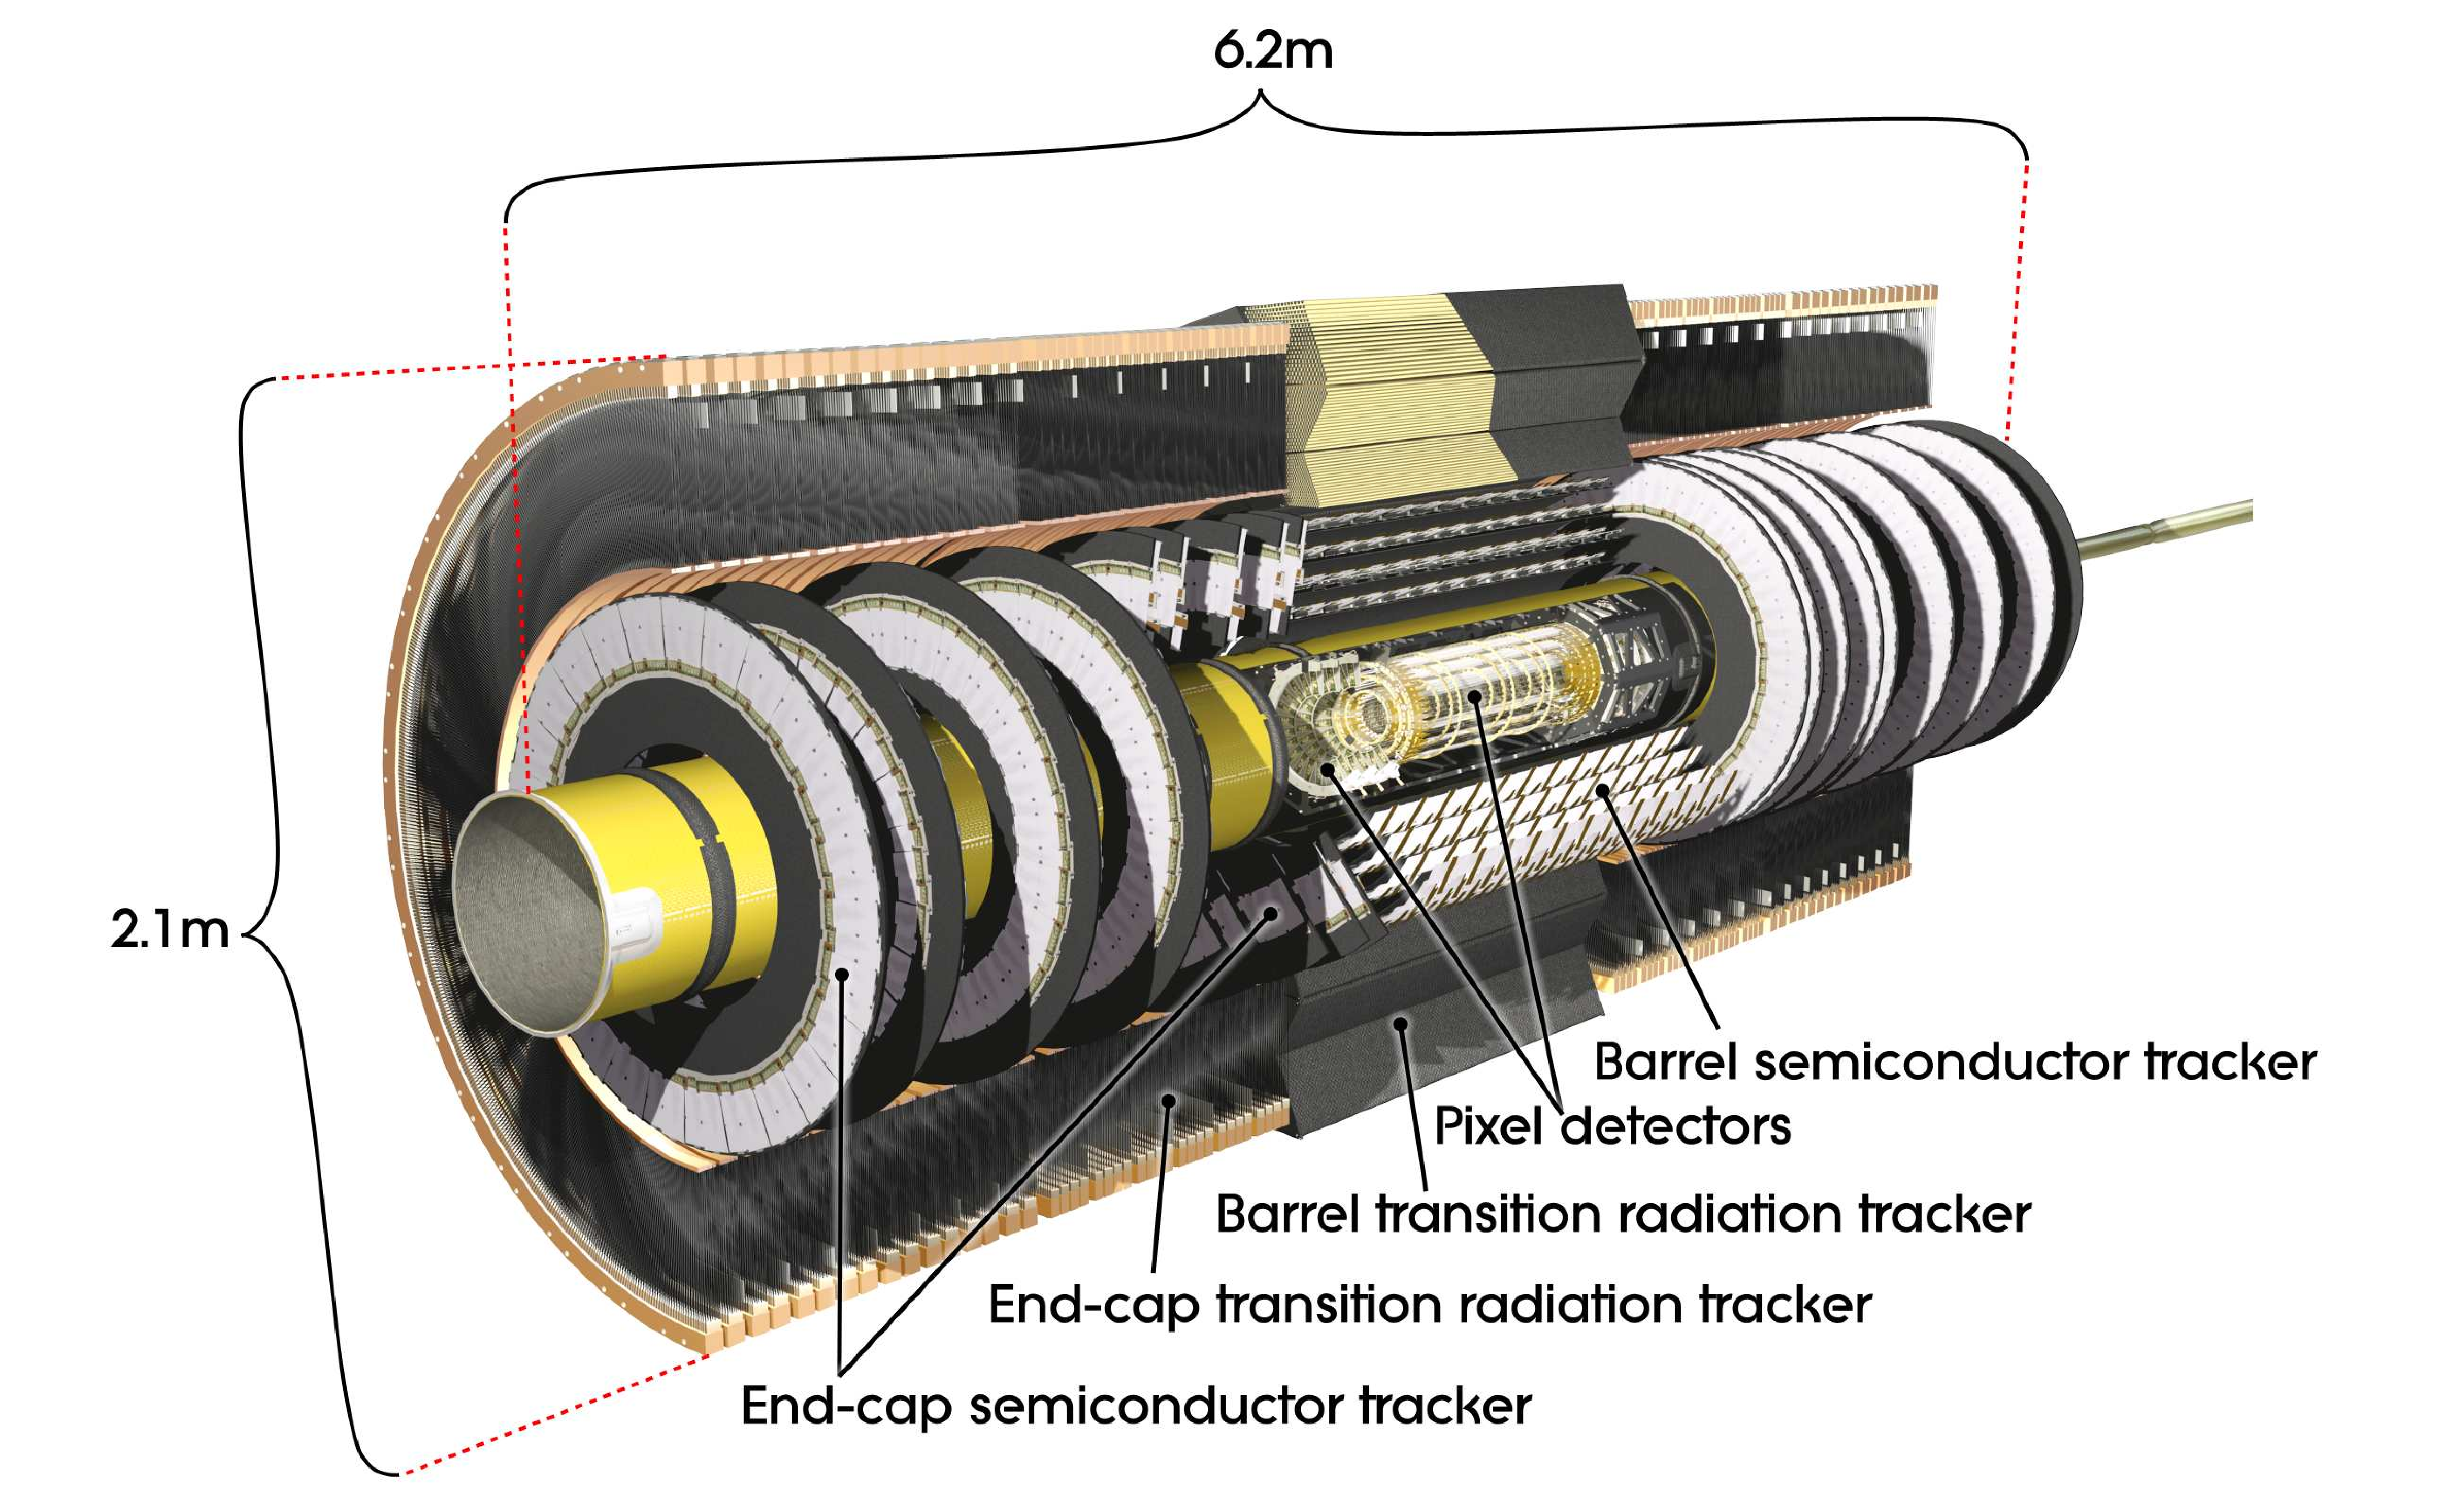
\includegraphics[width=\fullfig]{figures/id_overview.pdf}
%\caption{The arrangement of the subdetectors of the ATLAS inner detector. Each of the subdetectors is labeled in the cut-away view of the system.}
%\label{fig:id_overview}
%\end{figure}

\begin{figure}[hbtp]
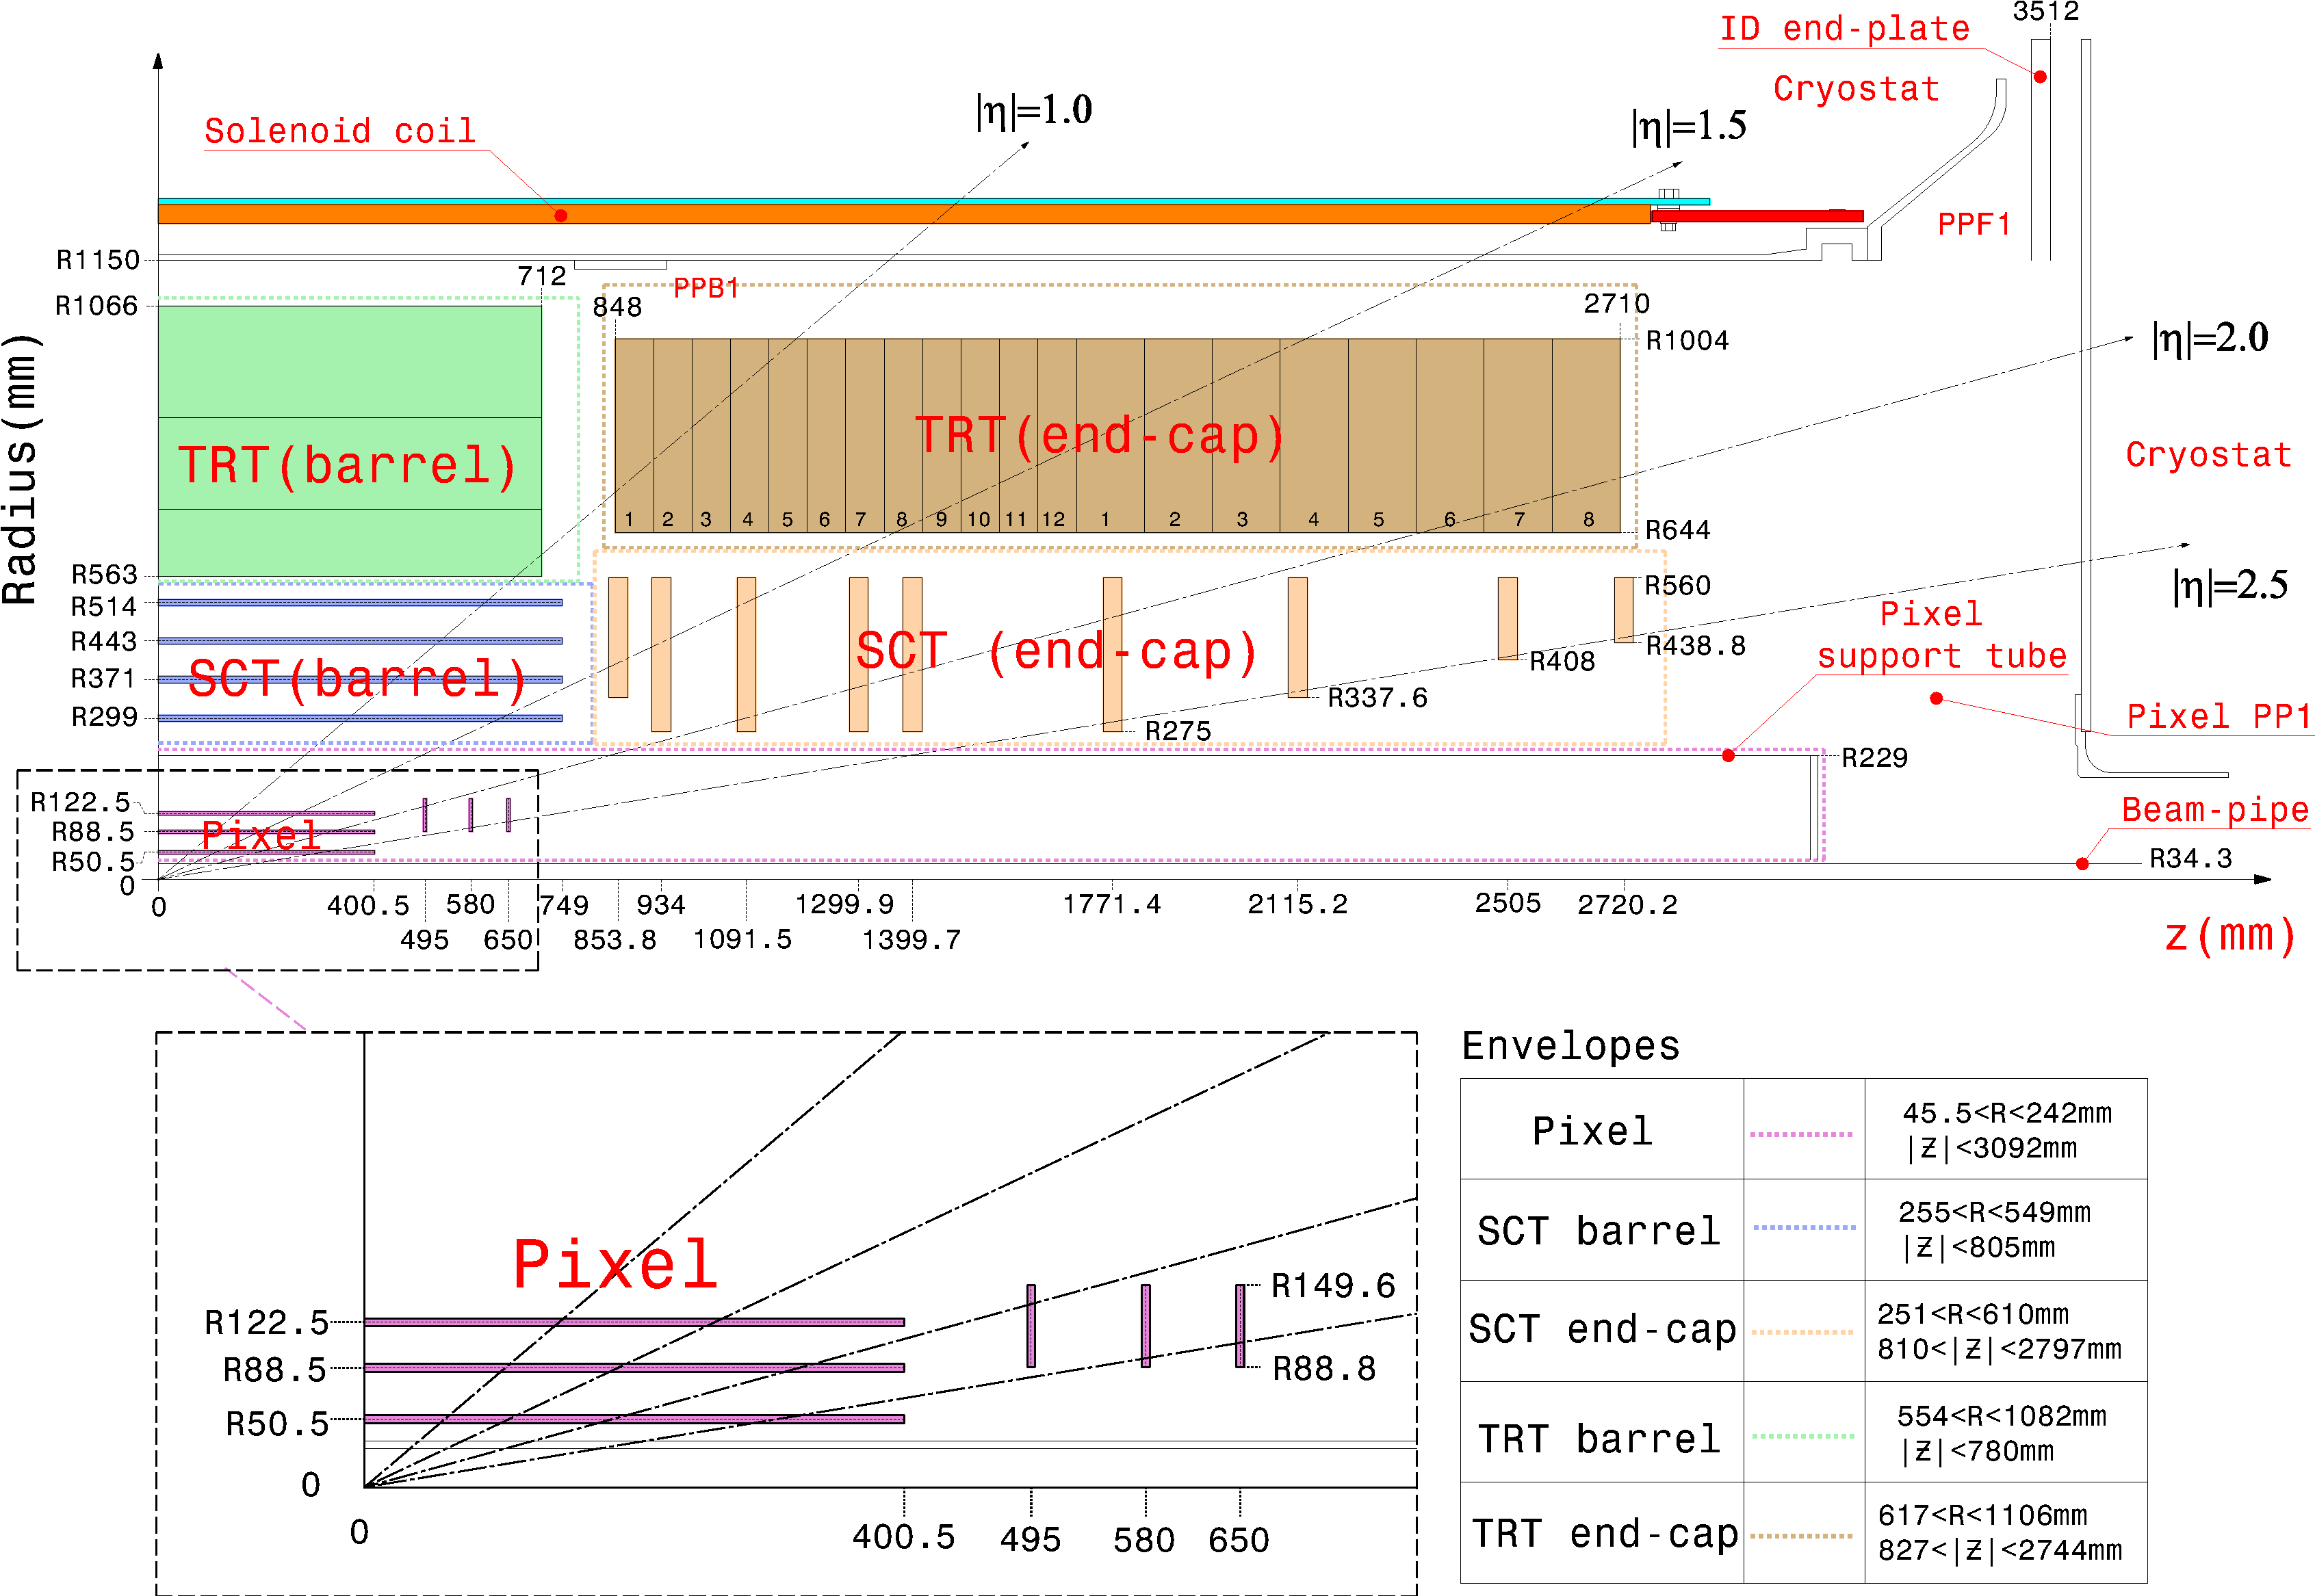
\includegraphics[width=\fullfig]{figures/id_detail_schematic.pdf}
\caption{A quarter section of the ATLAS inner detector which shows the layout of each of the subdetectors in detail. The lower panel shows an enlarged view of the pixel detector. Example trajectories for a particle with $\eta = 1.0, 1.5, 2.0, 2.5$ are shown. The \ac{IBL}, which was added after the original detector commissioning, is not shown.}
\label{fig:id_detail_schematic}
\end{figure}

Figure ~\ref{fig:id_slice} shows a computer generated three-dimensional view of the inner detector along the beam axis, which emphasizes the straw tube structure of the \ac{TRT} as well as the overlapping geometry of the \ac{SCT}.
This figure also includes the \ac{IBL}, which was added during the long shutdown and provides an additional measurement layer in the Pixel detector as of the beginning of Run 2. 
Figure ~\ref{fig:id_slice_long} shows an alternative computer generated three-dimensional view transverse to the beam axis which emphasizes the endcap structures of the \ac{SCT} and \ac{TRT}. 

\begin{figure}[hbtp]
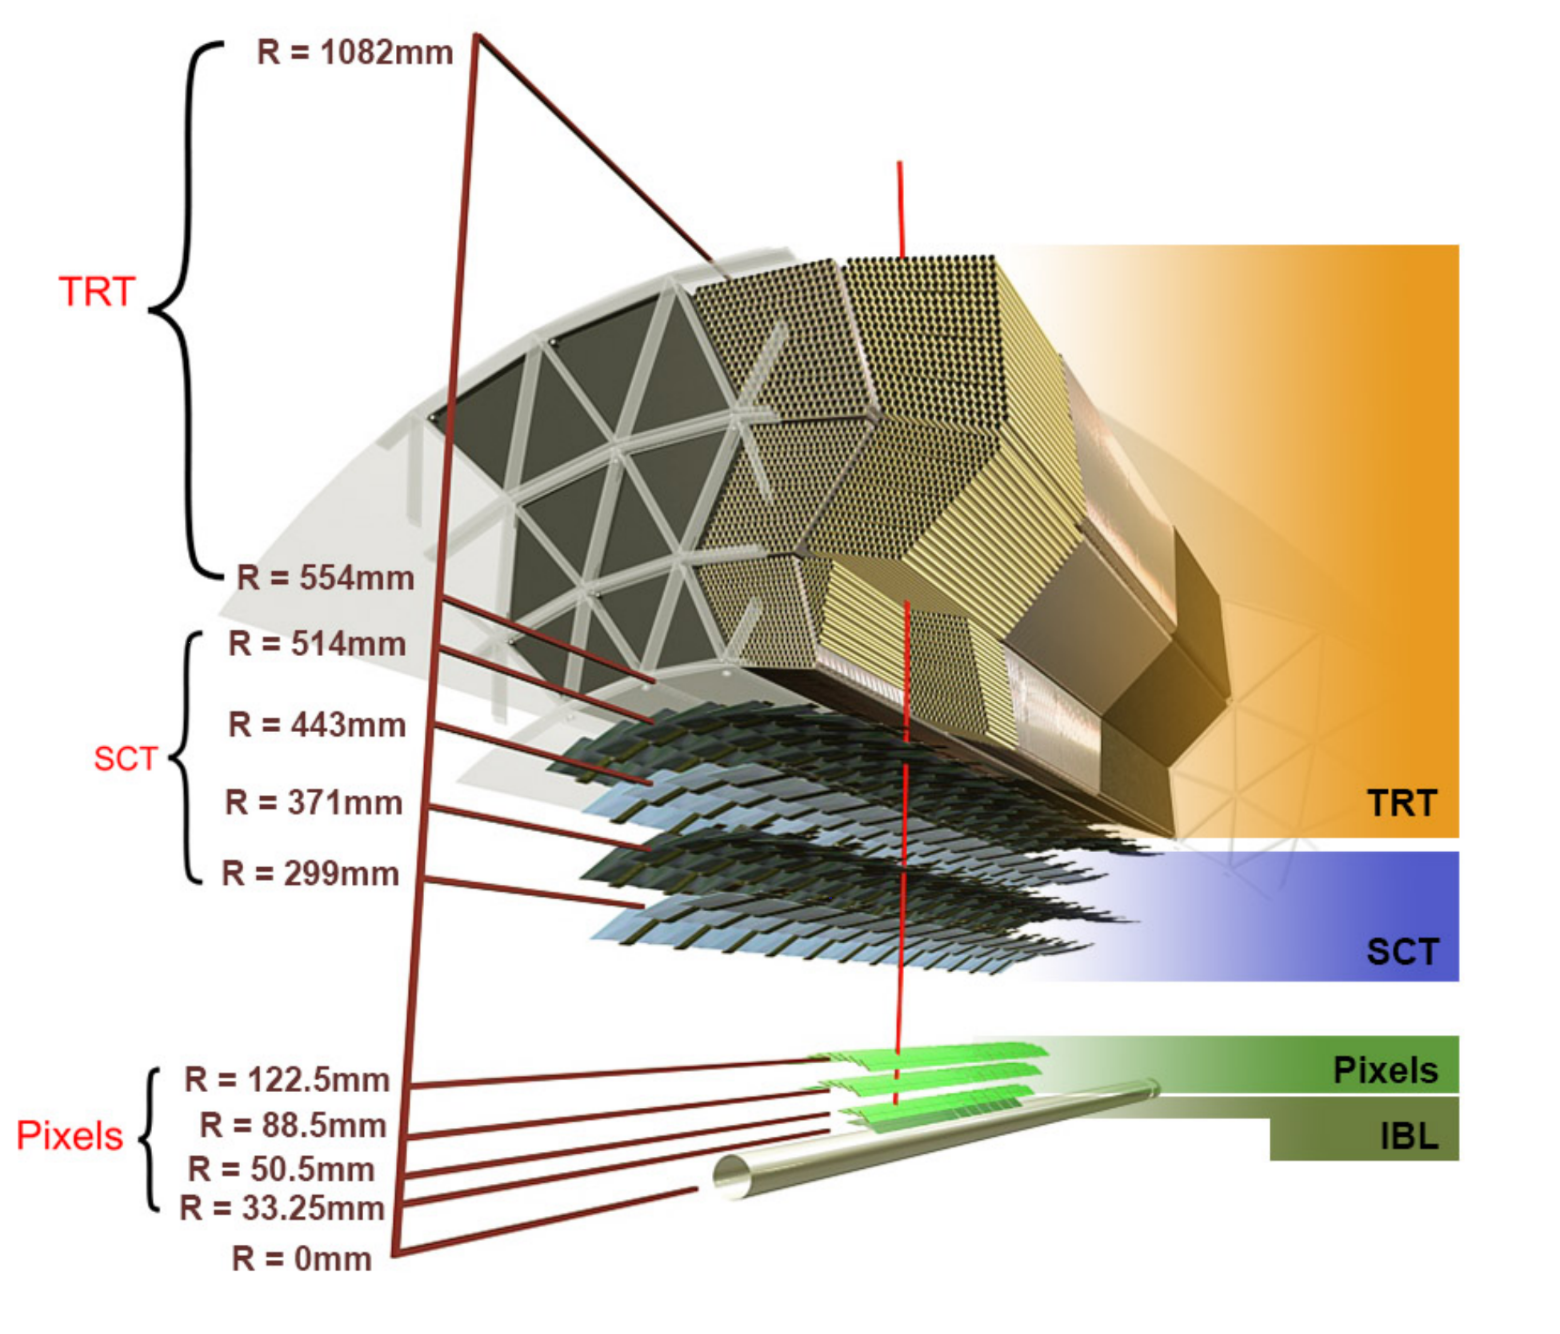
\includegraphics[width=\fullfig]{figures/id_slice.png}
\caption{A computer generated three-dimensional view of the inner detector along the line of the beam axis. The subdetectors and their positions are labeled.}
\label{fig:id_slice}
\end{figure}


\begin{figure}[hbtp]
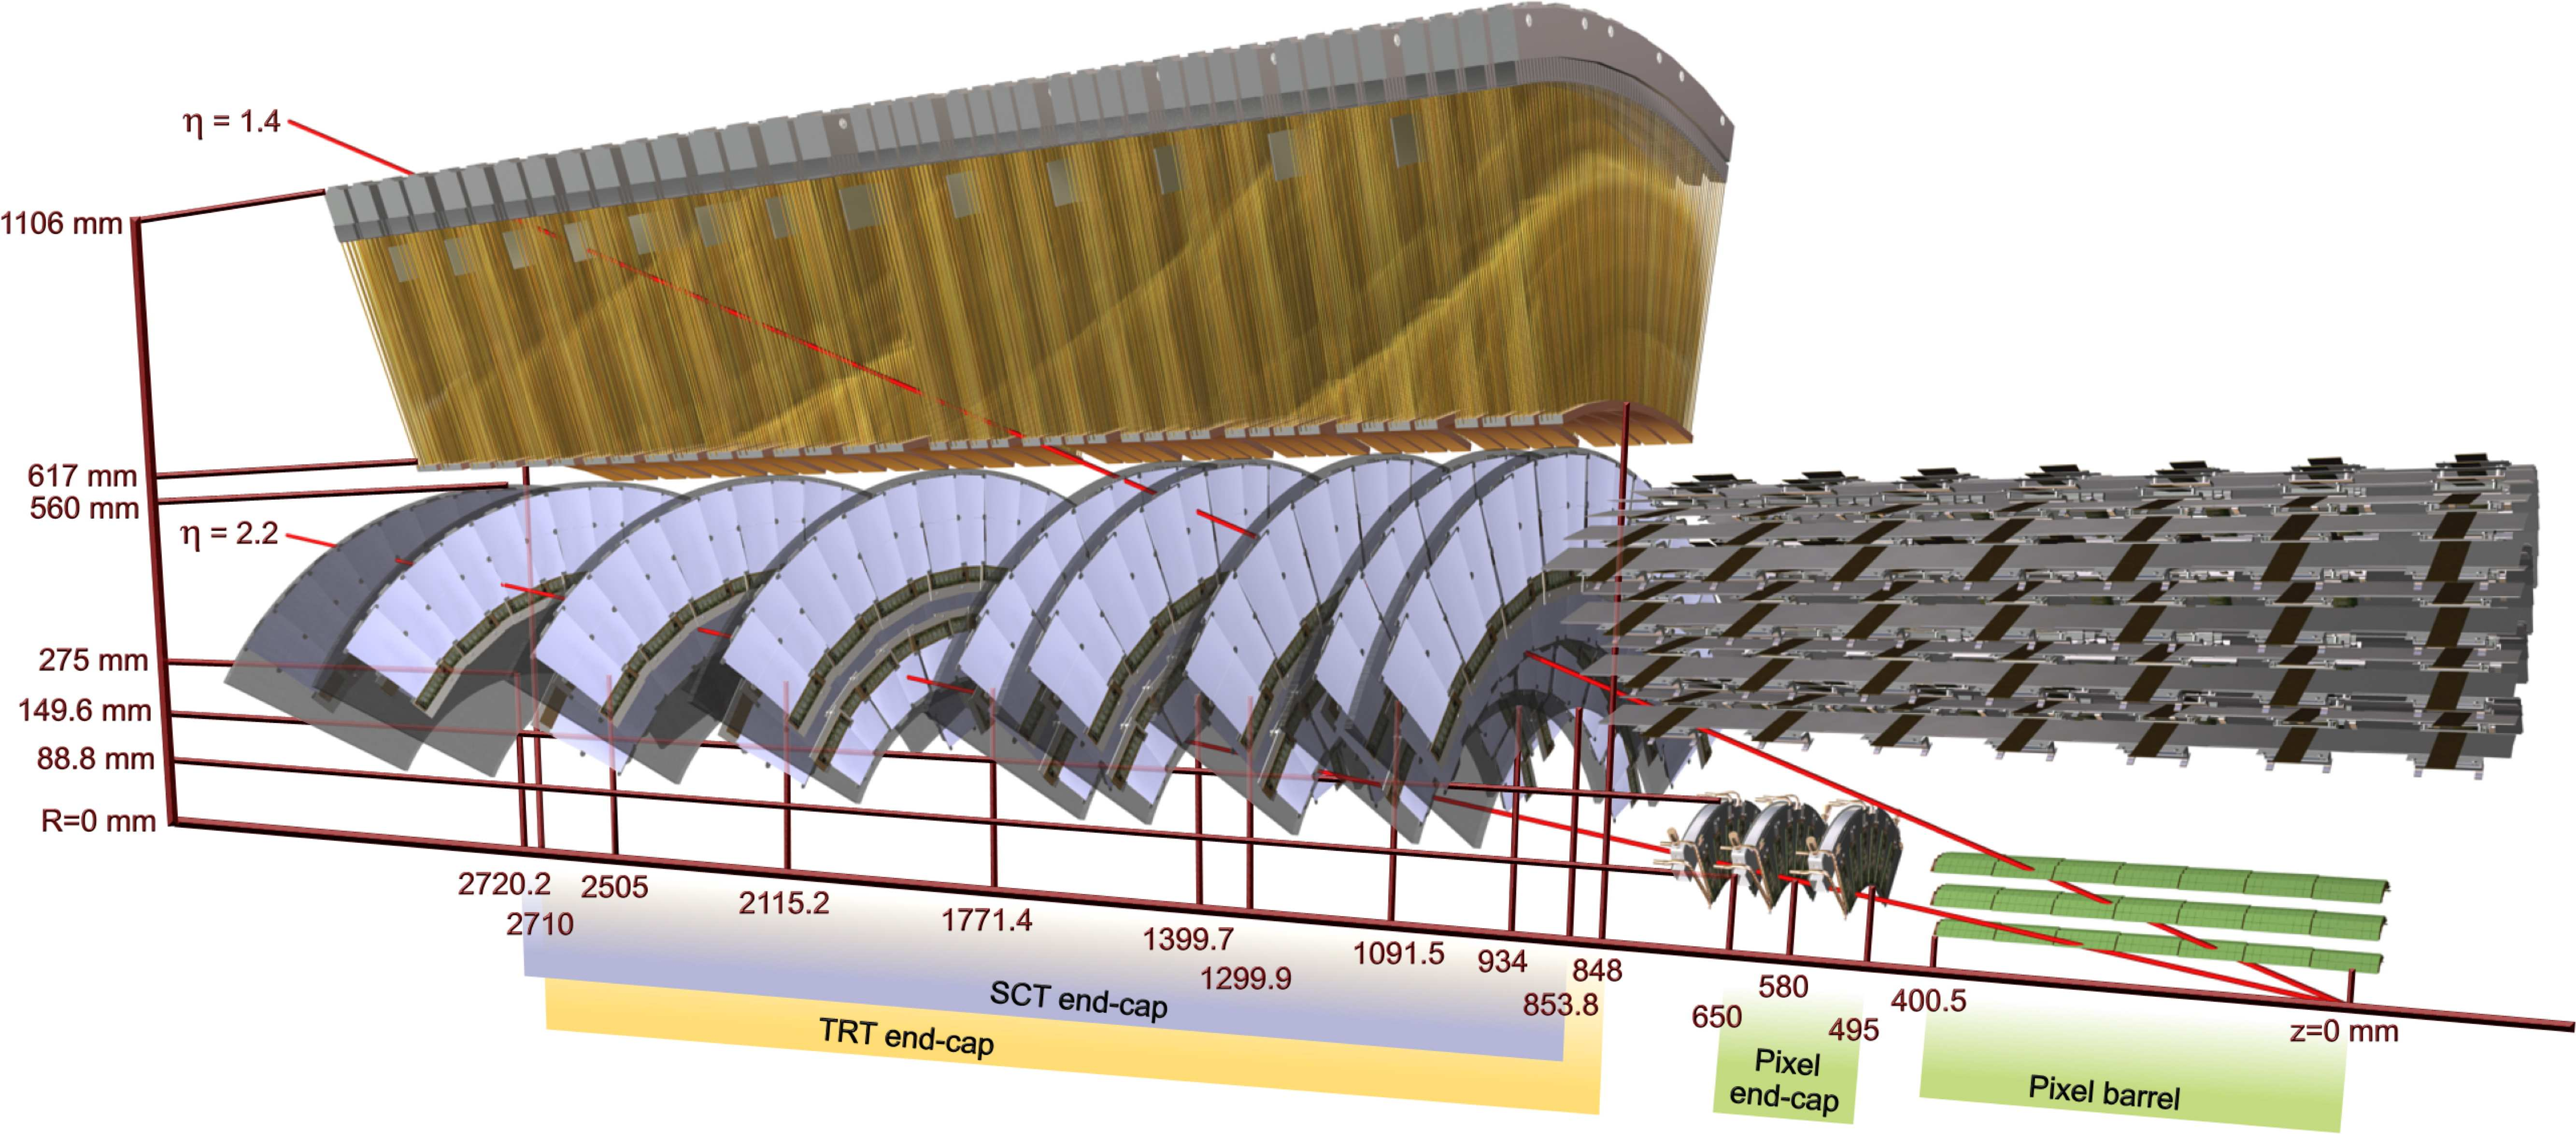
\includegraphics[width=\fullfig]{figures/id_slice_long.pdf}
\caption{An alternative computer generated three-dimensional view of the inner detector transverse to the beam axis. The subdetectors and their positions are labeled.}
\label{fig:id_slice_long}
\end{figure}

As the closest system to the interaction point, it is crucial for the inner detector to use as little material as possible to avoid scattering of charged particles before they reach the remaining subdetectors.
The various components, including the readout electronics, cooling infrastructure, gas volumes, and support structures,  were designed to accommodate this need for minimal components.
Even with these optimizations, the combination of stringent performance requirements and the harsh radiation environment in the inner detector requires a significant amount of material.
This material causes many electrons to lose most of their energy before reaching the electromagnetic calorimeter and approximately 40\% of photons convert into an electron-positron pair while traversing the inner detector.
Figure~\ref{fig:id_material} shows the integrated radiation lengths traversed by a straight track in the inner detector as a function of $\eta$, grouped by subdetector.
There is a large increase in the amount of material for support structures around $|\eta| = 1.7$, where the inner detector transitions from barrel to endcap.


\begin{figure}
\centering
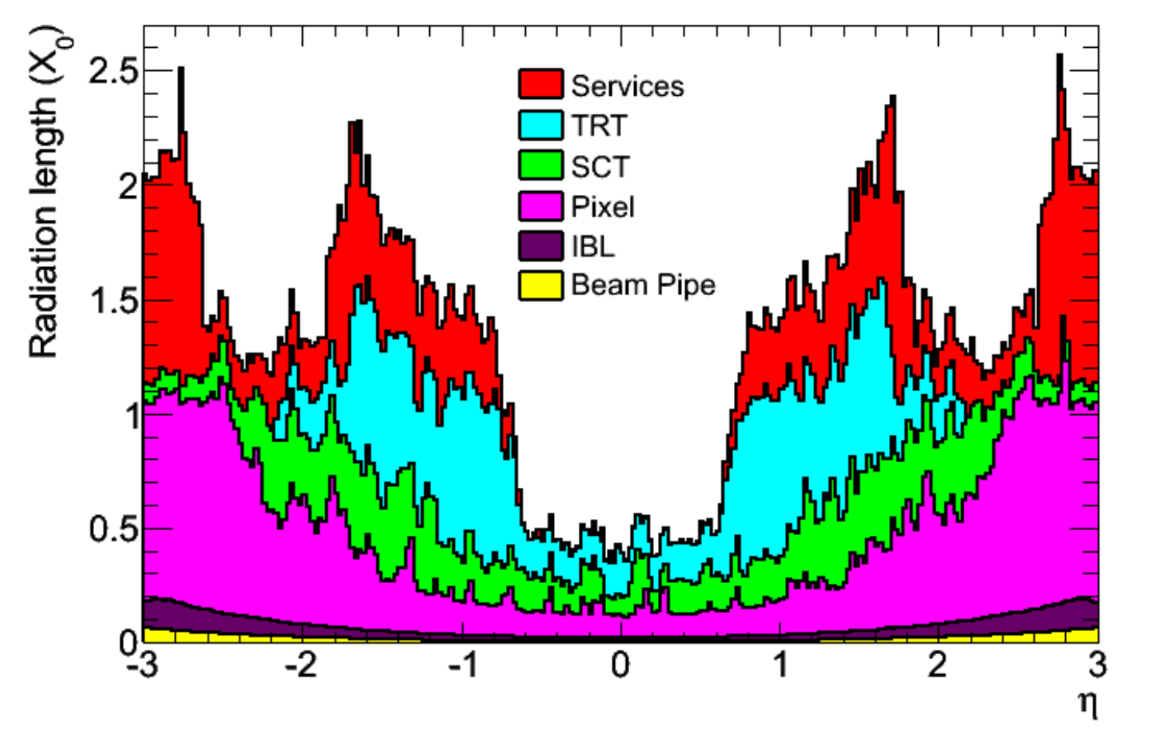
\includegraphics[width=\fullfig]{figures/id_material_subdetector.png}
\caption{The integrated radiation lengths traversed by a particle at the exit of the ID envelope (outside of the \ac{TRT} after 108.2 cm), including the services and thermal enclosures. The distribution is shown as a function of $|\eta|$ and averaged over $\phi$. The breakdown indicates the contributions of individual sub-detectors, including services in their active volume.}
\label{fig:id_material}
\end{figure}

The inner detector is designed to work as a cohesive unit to provide complete tracking information for charged particles.
Table~\ref{tab:id_parameters} summarizes the parameters of each of the subdetectors as well as the parameters of the combined inner detector. 

\begin{table}[h]
\begin{tabular}{lcccc}
\hline
Parameter & Inner Detector & Pixel & \ac{SCT} & \ac{TRT} \\
\hline
Inner Radius & 3.3 cm & 3.3 cm & 30 cm & 56 cm \\
$|\eta|$ Coverage & - & 2.5 & 2.5 & 2.0 \\
Cell Width & - & 50 \um & 80 \um & 4 mm \\
Cell Length & - & 400 \um & 12 cm & 70 cm \\
Material at $|\eta| = 0.0$ & 0.3 $X/X_0$ & & & \\
Material at $|\eta| = 1.7$ & 1.2 $X/X_0$ & & & \\
Material at $|\eta| = 2.5$ & 0.5 $X/X_0$ & & & \\
\hline
Number of Hits & 48 & 4 & 8 & 36 \\
Channels & 99 M & 92 M & 6.3 M & 350 k \\
\hline
\end{tabular}
\caption{A summary of the parameters of the inner detector and each of the subdetectors~\cite{atlas_experiment}.}
\label{tab:id_parameters}
\end{table}

%\begin{table}[h]
%\begin{tabular}{lll}
%\hline
%Parameter & Particle & Value \\
%\hline
%Reconstruction Efficiency & Muon, $\pt = 1\ \GeV$ & 96.8\% \\
%  & Pion, $\pt = 1\ \GeV$ & 84.0\% \\
%  & Electron, $\pt = 5\ \GeV$ & 90.0\% \\
%Momentum Resolution & $\pt = 1\ \GeV$, $|\eta| \approx 0$ & 1.3\% \\
%  & $\pt = 1\ \GeV$, $|\eta| \approx 2.5$ & 2.0\% \\
%  & $\pt = 100\ \GeV$, $|\eta| \approx 0$ & 3.8\% \\
%  & $\pt = 100\ \GeV$, $|\eta| \approx 2.5$ & 11\% \\
%Transverse \acs{IP} Resolution & $\pt = 1\ \GeV$, $|\eta| \approx 0$ & 75 \um \\
%  & $\pt = 1\ \GeV$, $|\eta| \approx 2.5$ & 200 \um \\
%  & $\pt = 1000\ \GeV$, $|\eta| \approx 0$ & 11 \um \\
%  & $\pt = 1000\ \GeV$, $|\eta| \approx 2.5$ & 11 \um \\
%Longitudinal \acs{IP} Resolution & $\pt = 1\ \GeV$, $|\eta| \approx 0$ & 150 \um \\
%  & $\pt = 1\ \GeV$, $|\eta| \approx 2.5$ & 900 \um \\
%  & $\pt = 1000\ \GeV$, $|\eta| \approx 0$ & 90 \um \\
%  & $\pt = 1000\ \GeV$, $|\eta| \approx 2.5$ & 190 \um \\
%\hline
%\end{tabular}
%\caption{A summary of the expected performance of the combined inner detector~\cite{gpd_lhc}. Included are the reconstruction effiencies for multiple particle types as well as the momentum and \ac{IP} resolution for various momenta.}
%\label{tab:id_performance}
%\end{table}


\subsection{Pixel Detector}
\label{sec:pixel}
The Pixel detector is the closest detector to the interaction point and therefore is designed to provide high granularity while simultaneously handling a large dose of radiation from collisions.
It consists of four layers of silicon pixel modules, each of which provides a precision measurement on the trajectory of any charged particle.
In the barrel region, the four layers are located at radial distances of 33 mm, 50.5 mm, 88.5 mm, and 122.5 mm. 
The three outer layers also include endcap elements, illustrated in Figure~\ref{fig:id_detail_schematic}, which are located at $z=495$ mm, $z=580$ mm, and $z=650$ mm away from the interaction point. 

The pixel sensor technology uses a p-n junction of n-type bulk that contains both p\tsup{+} and n\tsup{+} impurities.
This combination is crucial in maintaining performance after a significant radiation dose, as the n\tsup{+} implants allow the sensor to continue function after the n-type bulk has been converted to a p-type bulk by the accumulation of radiation.
In either configuration, when a charged particle passes through the bulk, it ionizes thousands of electron-hole pairs. 
The electrons and holes are pulled in opposite directions by the electric field established between the anode and cathode of the junction, which then produces a current that can be measured and recorded by readout electronics.

The size of the pixels in the original three layers are 50 \um x 400 \um in the $r-\phi$ and $z$ directions, respectively.
Those pixels are bump-bonded to front-end readout chips, the FE-I3, which contains a total of 2880 pixels per chip. 
In the three original pixel layers, the chips are grouped into modules composed of 16 chips each with 46,080 pixels per module and a total size of 20 mm x 60 mm x 250 \um. 
The modules are further arranged into long rectangular structures that run parallel to the beamline called staves.
By tiling several staves with an offset of 20\textdegree, the stave geometry provides full azimuthal coverage in the barrel region while accommodating the readout and cable systems.
The endcap regions are instead arranged into petals and then into wheels. 
This arrangement can be seen in Figure~\ref{fig:pixel_overview} which shows a computer-generated, cut-away image of the outer three layers of the pixel detector.
Together these three layers contain 1744 modules between the barrel and two endcap sections.

\begin{figure}[hbtp]
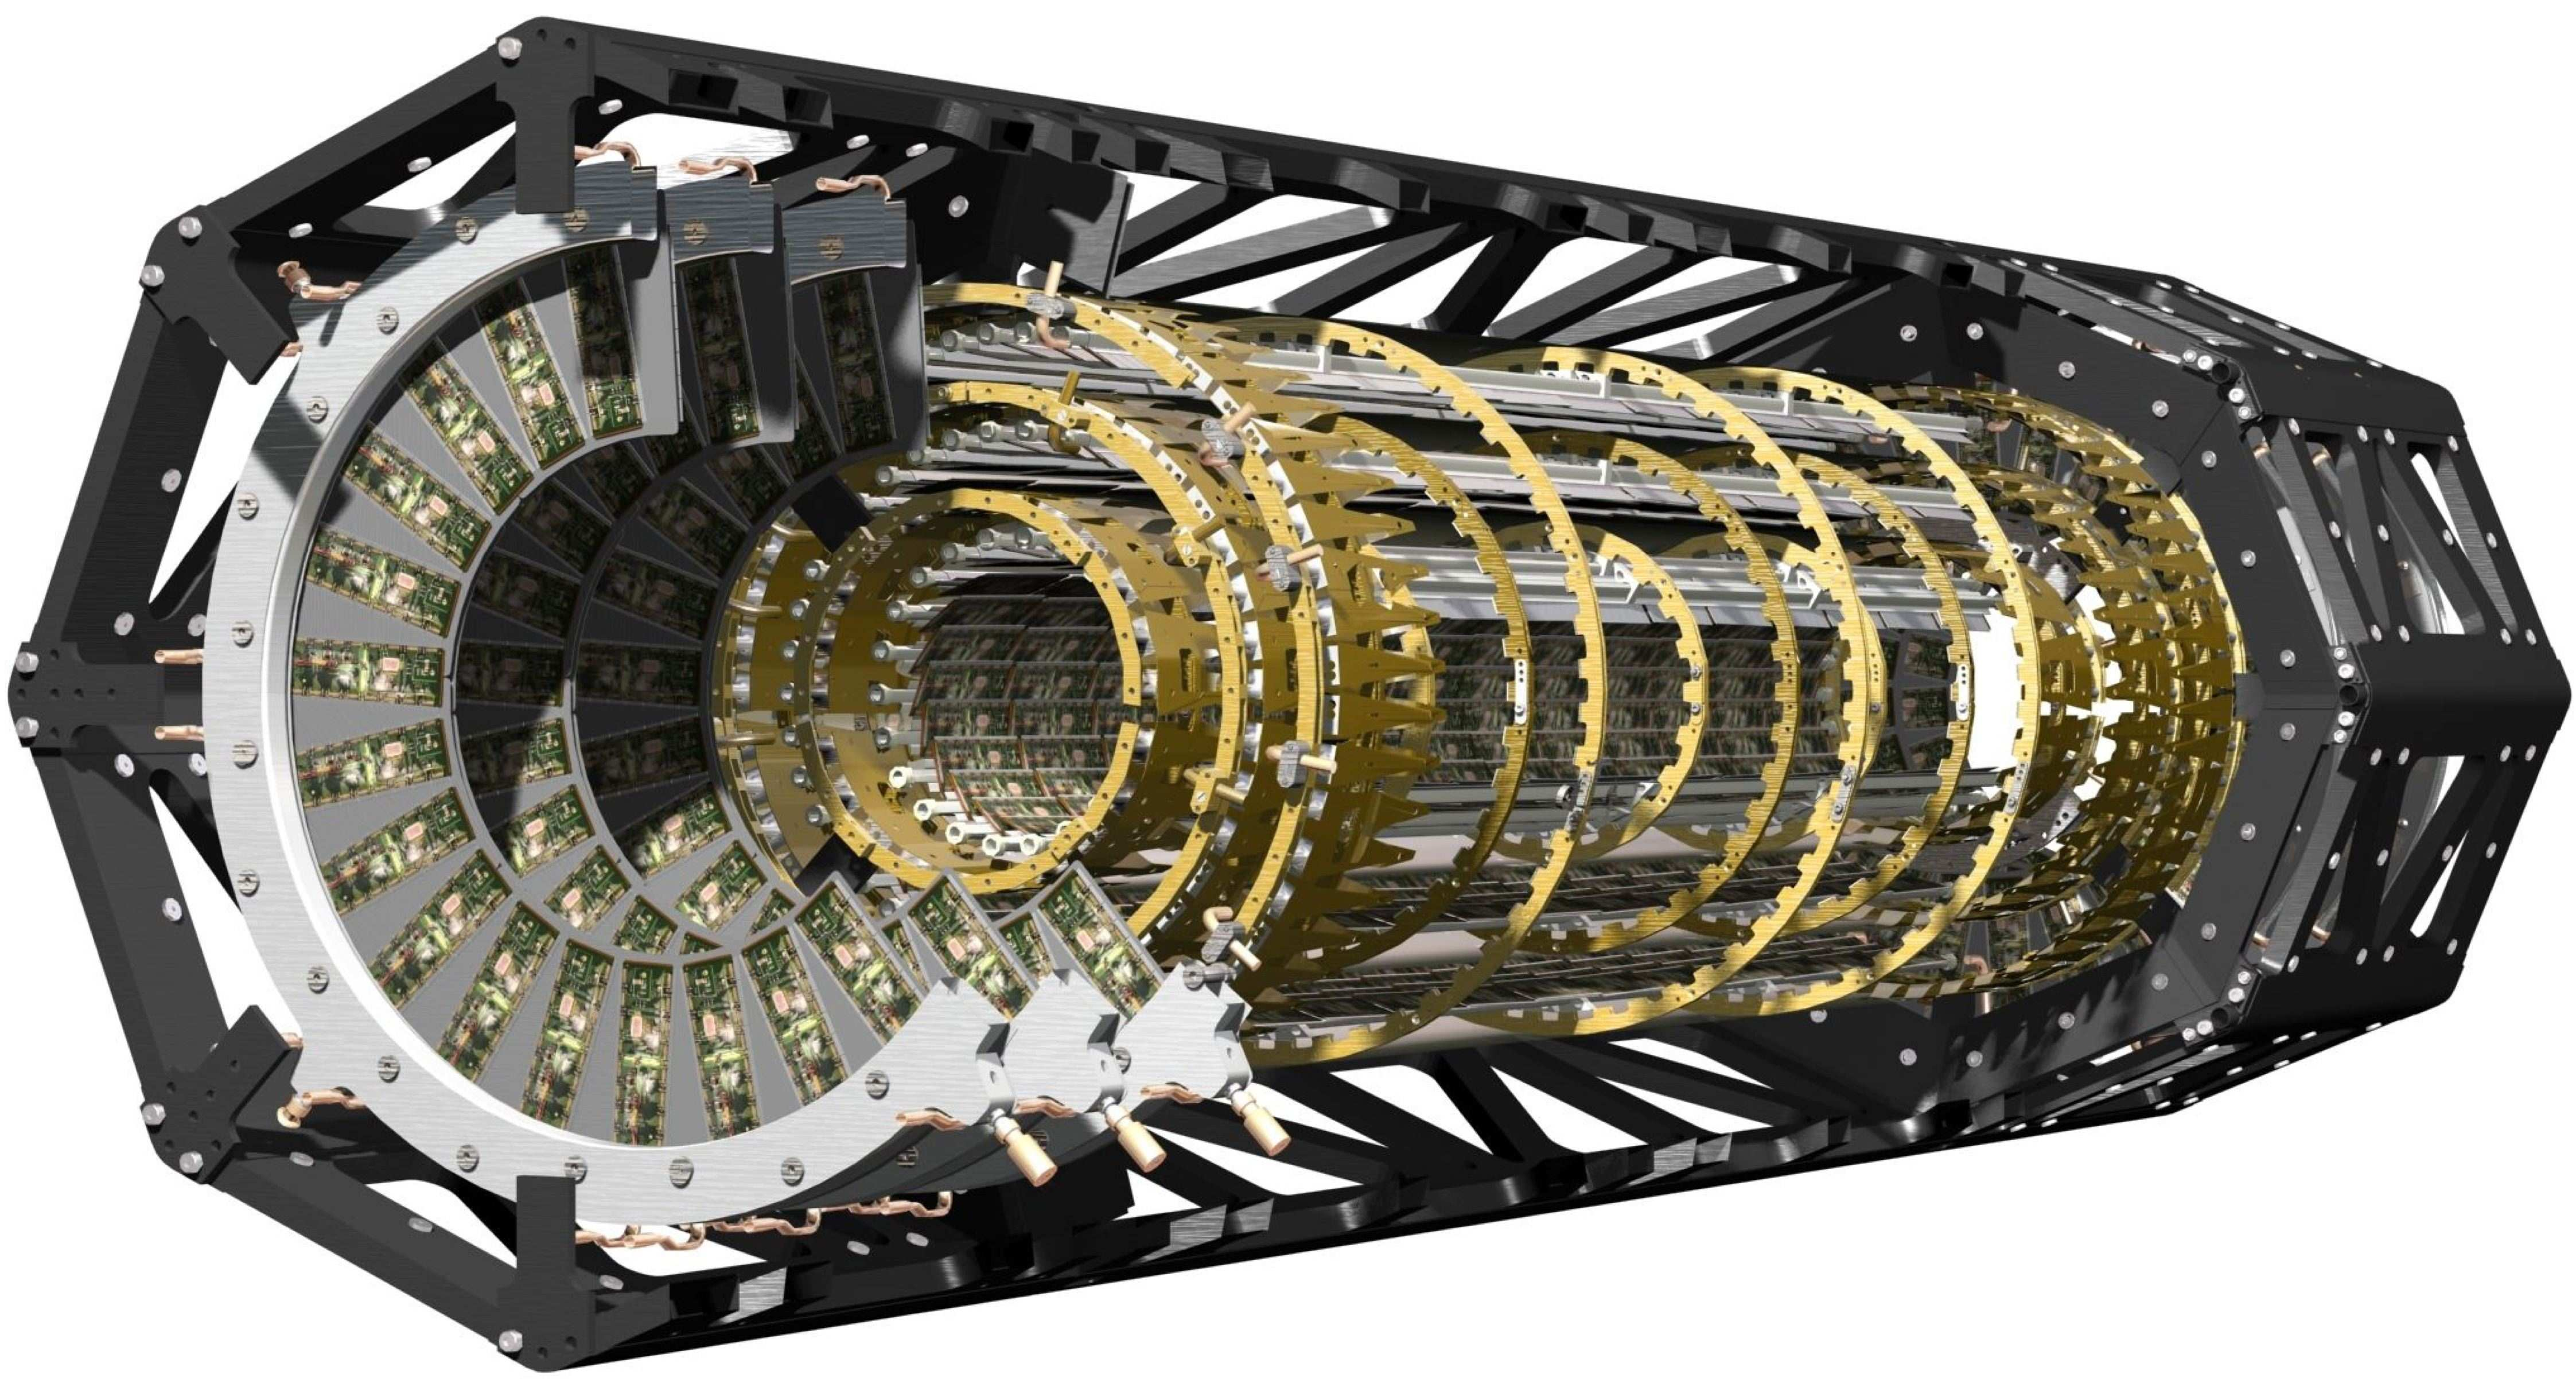
\includegraphics[width=\fullfig]{figures/pixel_overview.pdf}
\caption{A cut away image of the outer three layers of the pixel detector.}
\label{fig:pixel_overview}
\end{figure}

The innermost layer, the \ac{IBL}, was added during the long shutdown before Run 2, and provides the fourth track measurement.
It was inserted directly into the existing pixel detector by removing the existing beam pipe and replacing it with a significantly smaller version.
This insertion can be seen in action in Figure~\ref{fig:ibl_insertion}, which emphasizes the extreme precision required to place the the 70 cm long layer with only 2 mm of clearance.
The \ac{IBL} was commissioned to provide continued tracking robustness and high precision in the higher luminosity environment of Run 2~\cite{ibl_tdr}.
The proximity of this layer to the collisions necessitated an even higher granularity and better radiation hardness than the other pixel layers.
And the strict space requirements to add an active sensing layer so close to the interaction point required a sensor chip with a much higher active area and a larger overall area per chip.
These requirements led to the development of a new chip type, the FE-I4 (compared to the FE-I3 chips used in the original pixel detector) with improved radiation hardness and a larger active area.
The \ac{IBL} is comprised of 448 of these individual chips arranged in 14 staves, with 26,880 pixels per chip and a chip size of 18.5 mm x 41.3 mm x 200 \um.
The staves, like in the other layers of the pixel detector, are offset by $14^\circ$ to provide full azimuthal coverage.
This arrangement can be seen in Figure~\ref{fig:ibl_geometry}, which shows two computer-generated images of the \ac{IBL} geometry and includes the some of the remaining pixel layers.


\begin{figure}[hbtp]
\centering
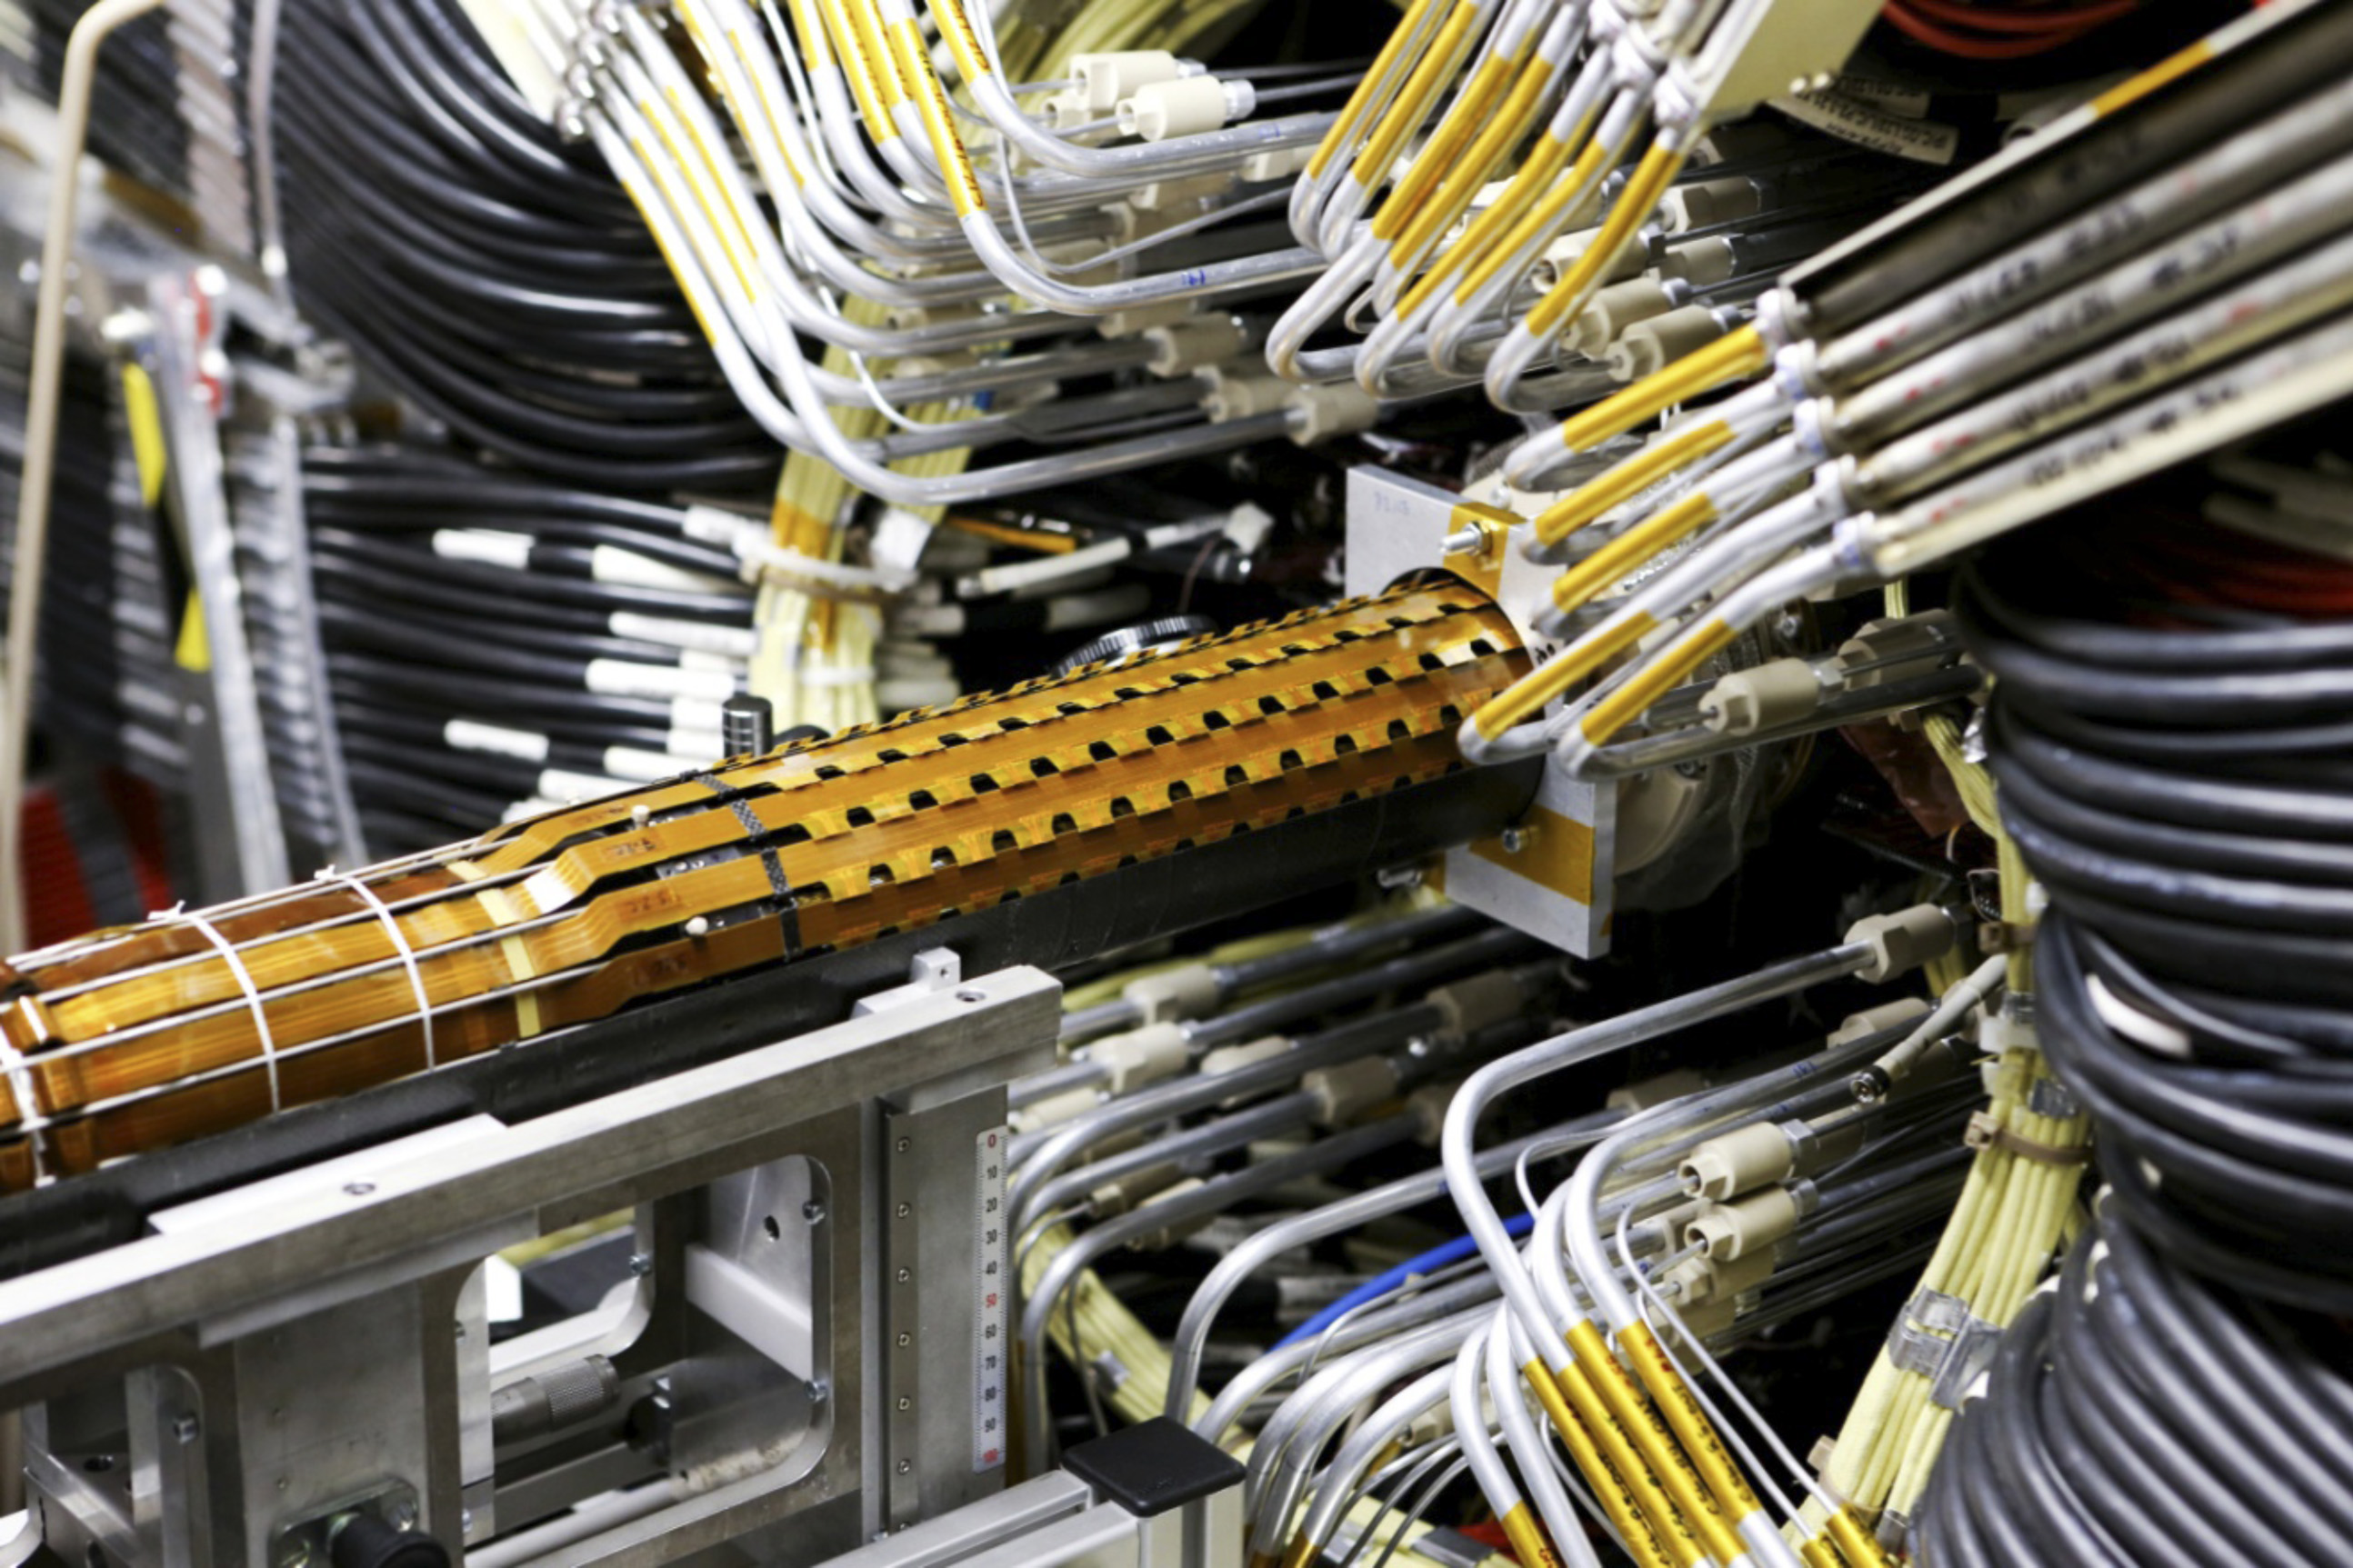
\includegraphics[width=\fullfig]{figures/ibl_insertion.jpg}
\caption{An image of the insertion of the \ac{IBL} into the current pixel detector.}
\label{fig:ibl_insertion}
\end{figure}


\begin{figure}[hbtp]
\centering
\subfloat[]{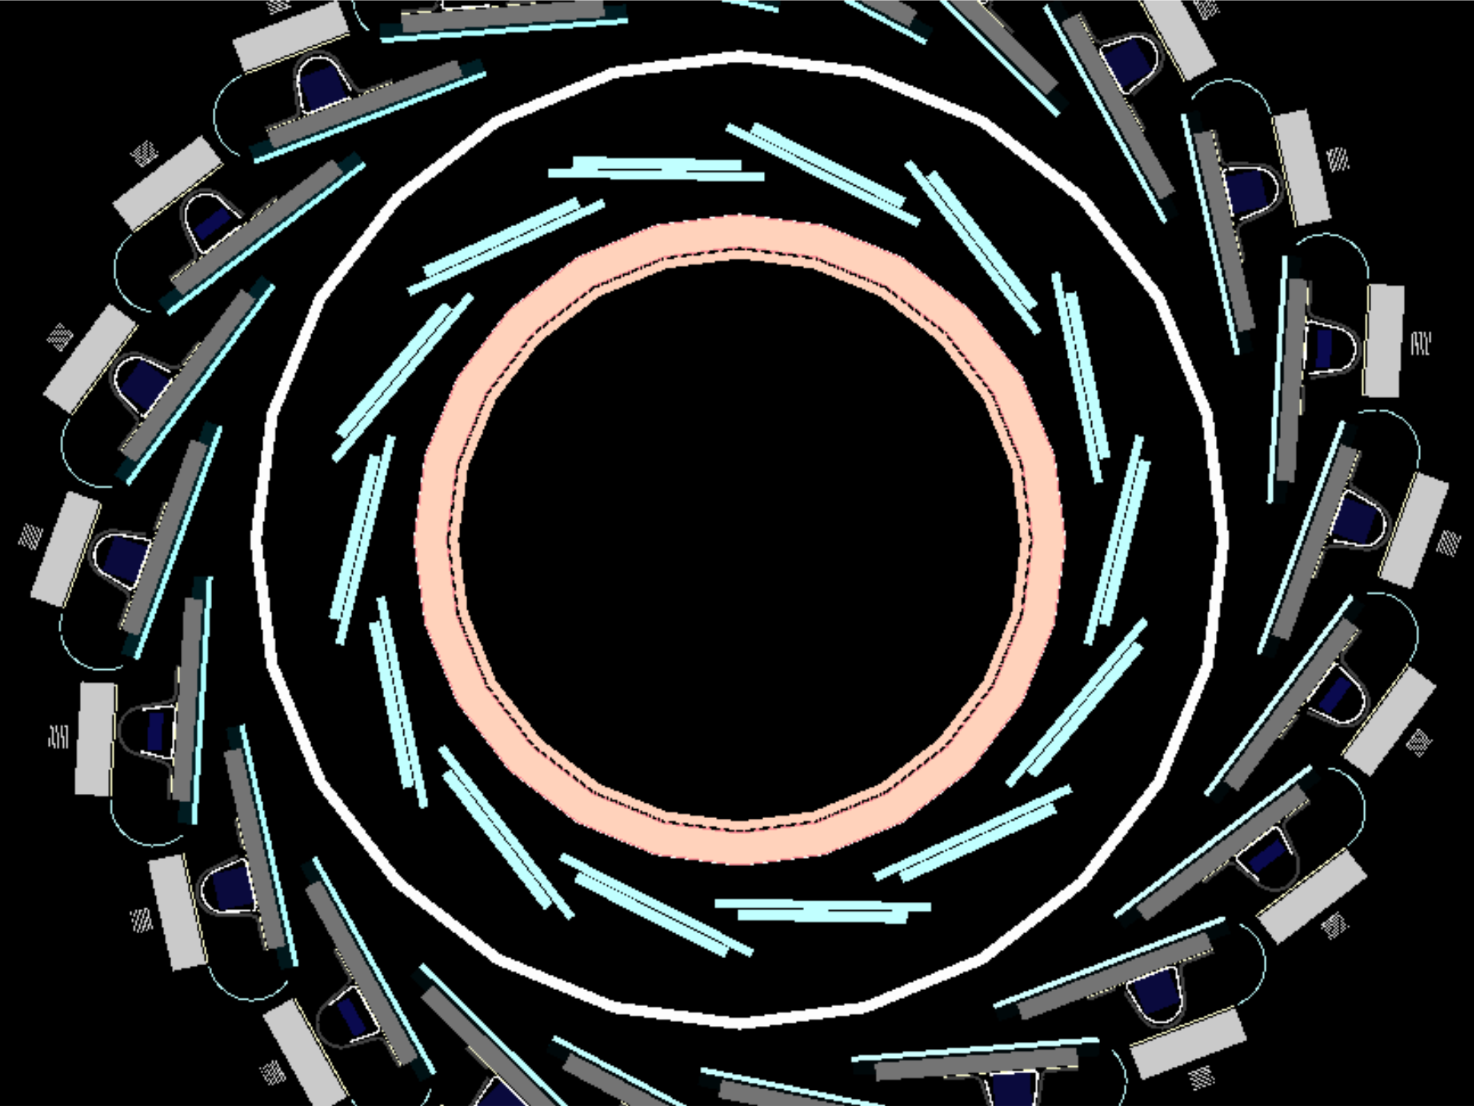
\includegraphics[width=\halffig]{figures/ibl_transverse.png}}\\
\subfloat[]{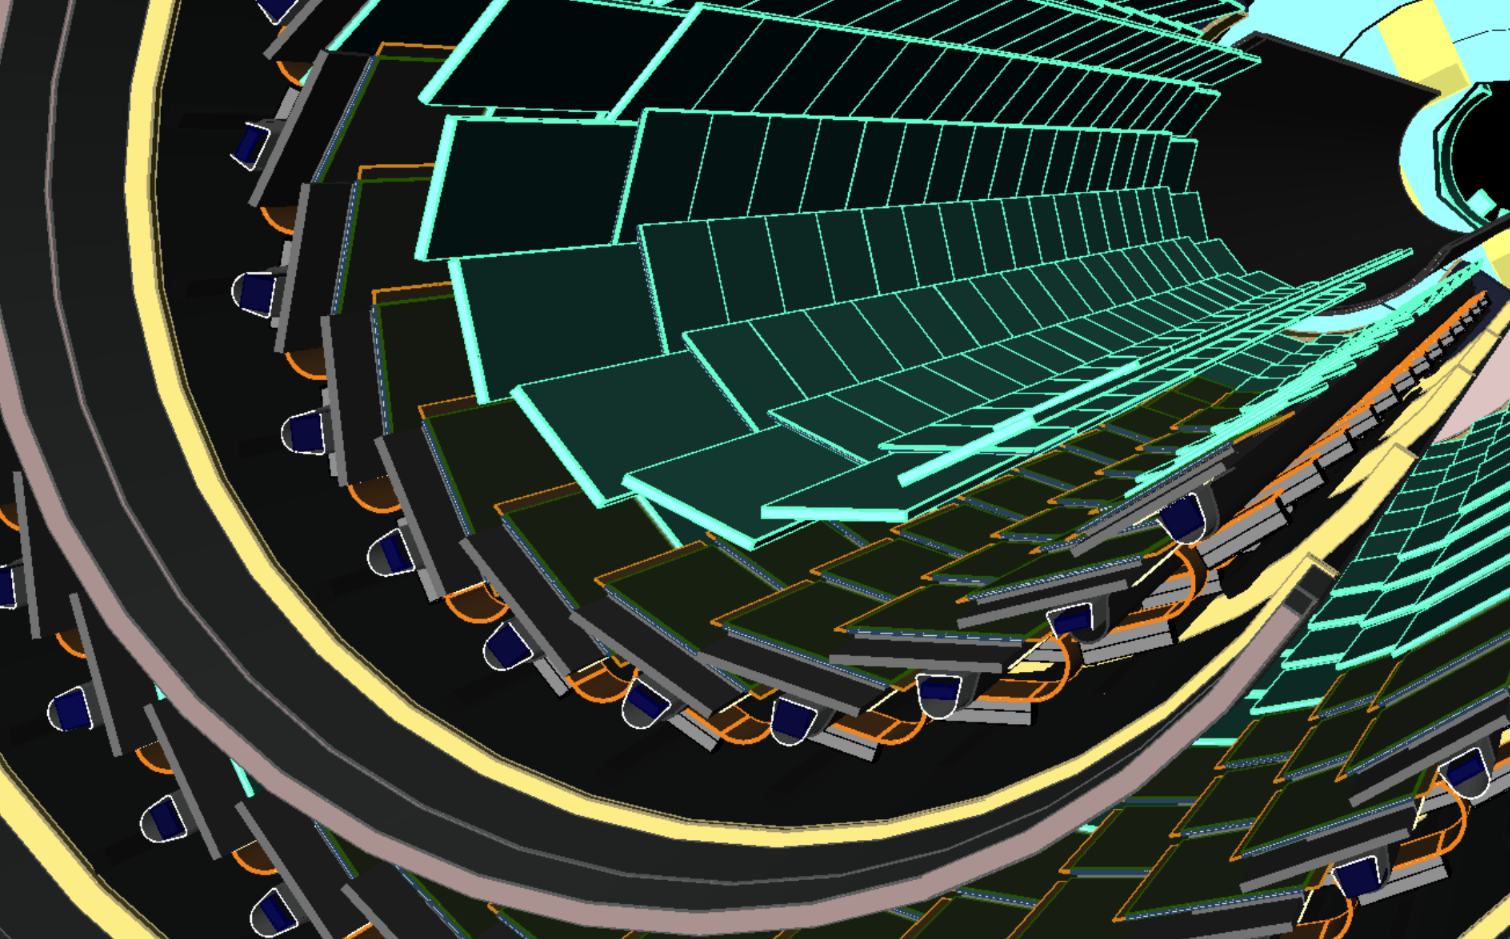
\includegraphics[width=\halffig]{figures/ibl_longitudinal.png}}
\caption{A three-dimensional computer-generated image of the geometry of the \ac{IBL} with a view (a) mostly transverse to the beam pipe (b) mostly parallel to the beam pipe.}
\label{fig:ibl_geometry}
\end{figure}

\subsection{Semiconductor Tracker}

The \ac{SCT}, the subdetector which immediately surrounds the Pixel detector, provides additional discrete measurements of the trajectory of a charged particle.
Because the \ac{SCT} is further away from the interaction point, the spatial resolution does not need to be as high as in the pixel detector, and so the \ac{SCT} uses micro-strips instead of pixels. 
Although pixels provide a more accurate measurement, the number of pixels and readout channels required to cover the cylindrical area at the radius of the \ac{SCT} layers would be prohibitively complicated and expensive.

Each individual silicon strip sensor contains 768 individual readout strips with a total area of 6.36 cm x 6.40 cm and a pitch of 80 \um. 
Pairs of these sensors are then bonded together to form a combined strip with a length of 12.8 cm.
Two of these combined strips are then placed back to back with a relative tilt of 40 mrad.
This geometry is illustrated in an expanded view in Figure~\ref{fig:sct_geometry}.
The purpose of angular offset of the consecutive layers is to allow the strip sensor areas to more accurately measure the position of a particle in the $z$ direction by comparing the overlap of the two strips which were traversed by a track.

\begin{figure}[hbtp]
\centering
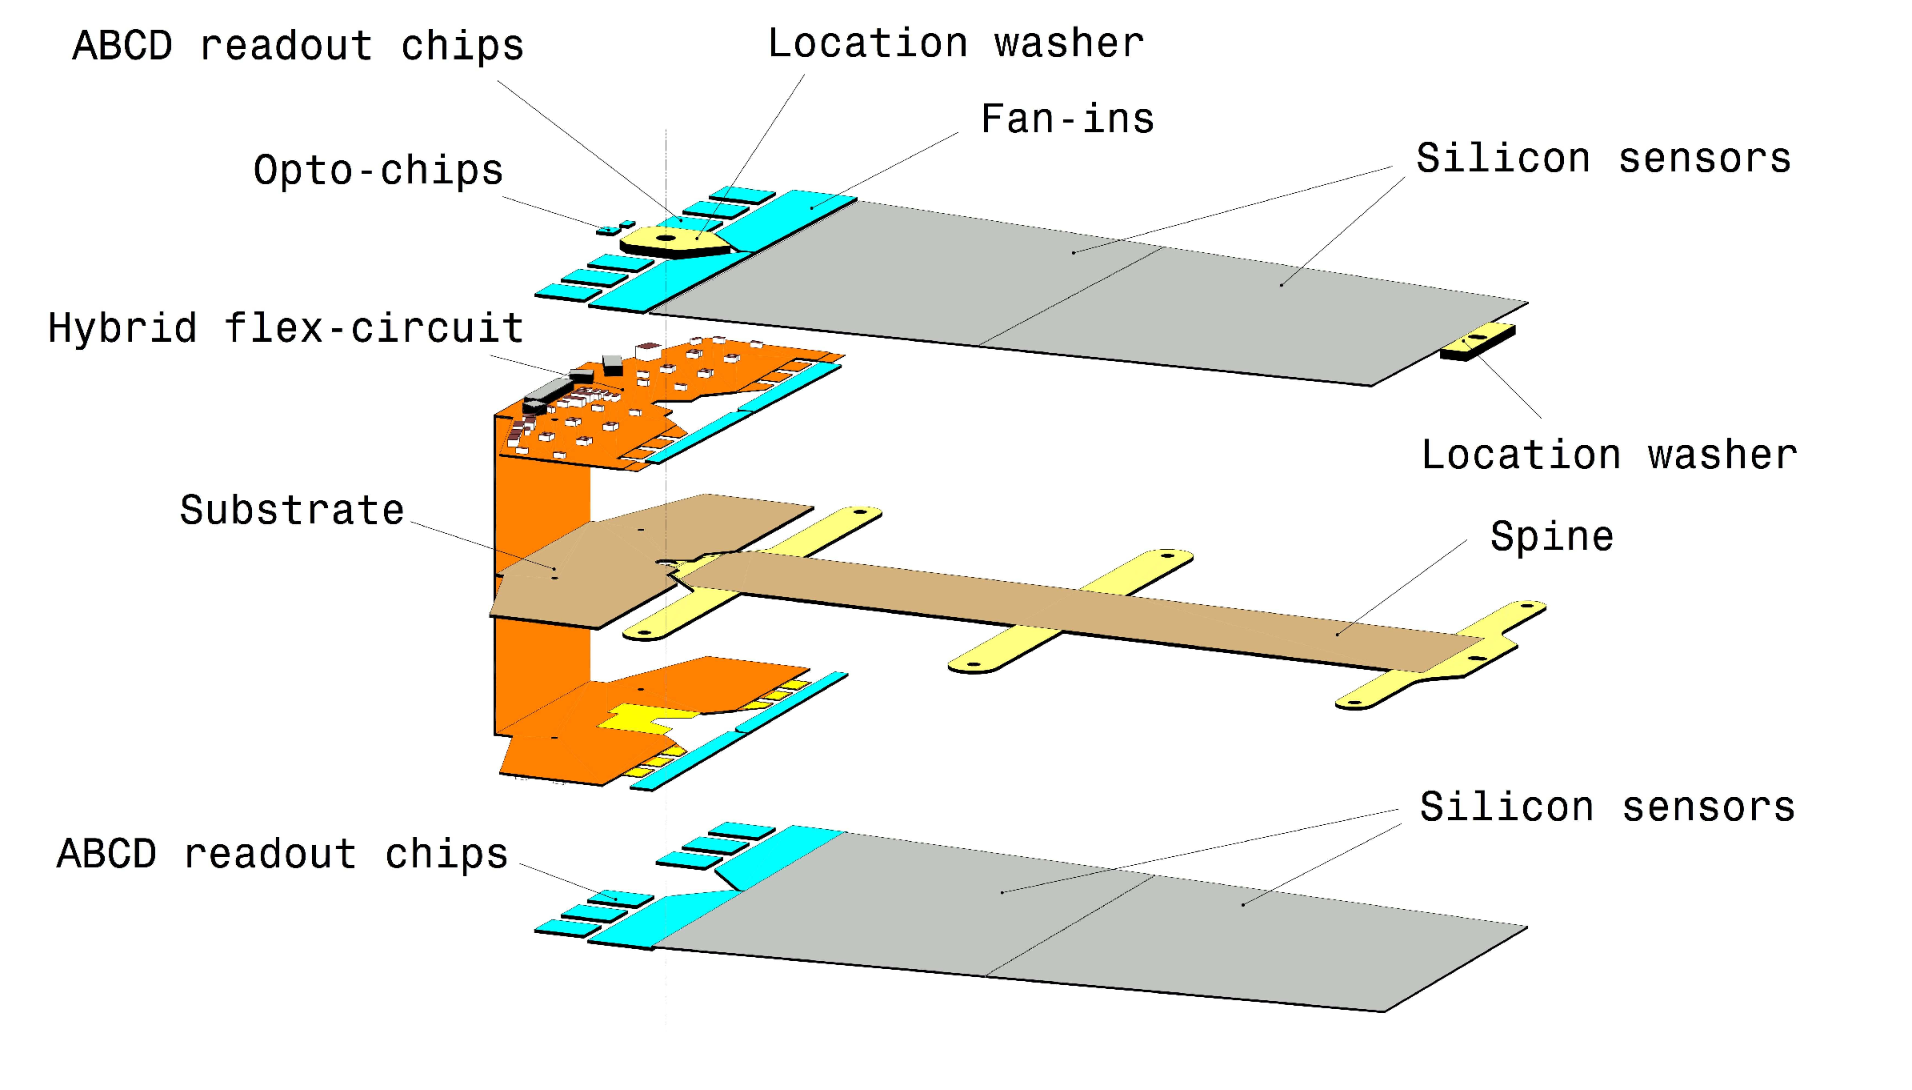
\includegraphics[width=\fullfig]{figures/sct_geometry.png}
\caption{An expanded view of the geometry of the \ac{SCT} double layers in the barrel region.}
\label{fig:sct_geometry}
\end{figure}

Four of these double layers are placed in the barrel region, with radii of 299 mm, 371 mm, 443 mm, and 514 mm. 
Together these layers provide eight additional measurements for each track that traverses the central $|\eta|$ region.
In the endcap region, the layers are arranged in wheels, with the double layers similarly offset to provide improved resolution.
With these configurations, the \ac{SCT} achieves a spatial resolution of 17 \um in the $r-\phi$ direction and 580 \um in the $z$ direction.

\subsection{Transition Radiation Tracker}

The final component of the inner detector, the \ac{TRT}, provides continuous tracking using straw drift tubes.
The tubes are made of Kapton and aluminum with a diameter of 4 mm and are filled with a gas mixture of 70\% Xe, 27\% CO\tsub{2}, and 3\% 0\tsub{2}. 
At the center of each tube is a gold-plated anode tungsten wire which is 30 \um in diameter.
When a charged particle passes through these tubes, it ionizes the gas within.
The ions produced drift in the electric field established between the wire and the tube wall, and the large electric field near the wire produces avalanche multiplication and results in an electric current on the wire that is read out by the electronics and provides a track measurement.
The time it takes the ionization to drift to the wire can be used to estimate the distance from the wire that the particle passed through the tube; this gives a resolution on the distance of approximately 130\um.
Combining several such measurements between consecutive hits in the \ac{TRT} tubes allows the trajectory of the particle to be reconstructed with much better resolution than is available in each individual tube.

In addition to the continuous tracking, the detector can use transition radiation produced when a particle passes between the layers to distinguish between electrons and heavier charged particles.
The space between the tubes is filled with CO\tsub{2}, and so has a different dielectric constant than the gas within the tubes which contains Xe.
At the transition between those media, a relativistic particle emits radiation proportional to $\gamma$, so inversely proportional to mass at a fixed momentum.
The photons produced in this transition then produces an ionization cascade which is significantly larger than the signal for the minimally-ionizing charged particles.
To distinguish between these two cases, the \ac{TRT} defines two signal thresholds, a low threshold for the typical signal produced by a \ac{MIP} and a high threshold for the the signal produced by transition radiation.
A high momentum electron is expected to produce approximately 7 to 10 high threshold hits as it traverses the \ac{TRT}, and thus these hits provide a way to distinguish electrons from other charged particles. 

The \ac{TRT} contains 351,000 tubes in total, divided between the barrel and endcap regions. 
In the barrel region, the tubes are 144 cm long and arranged in 73 layers parallel to the beampipe.
In the endcap region, the tubes are 37 cm long and arranged in 160 layers transverse to the beampipe.
These configurations can be seen in Figure~\ref{fig:id_slice} and Figure~\ref{fig:id_slice_long}. 
With this geometry the \ac{TRT} achieves a resolution of 130 \um  in the $r-\phi$ direction.

% ----------------------------------------

\section{Calorimetry}
\label{sec:calorimetry}

The combination of calorimeter systems used in ATLAS can measure the energy of electrons, photons, hadrons, and hadronic jets with complete coverage up to $|\eta| < 4.9$ and across $\phi$.
Unlike the inner detector, the calorimeters are capable of measuring neutral particles.
To accomplish precision measurements of these particle types, the ATLAS calorimeter system uses four individual calorimeters, a \ac{LAr} \acl{EM} calorimeter in the barrel region, a tile hadronic calorimeter in the barrel region, a \ac{LAr} hadronic endcap calorimeter, and a \ac{LAr} forward calorimeter.
Together these provide hermetic coverage for the ATLAS detector.
The configuration of these calorimeters is illustrated in Figure~\ref{fig:calo_overview}. 
%Table~\ref{tab:calorimeter_parameters} summarizes the parameters of these systems.

\begin{figure}[hbtp]
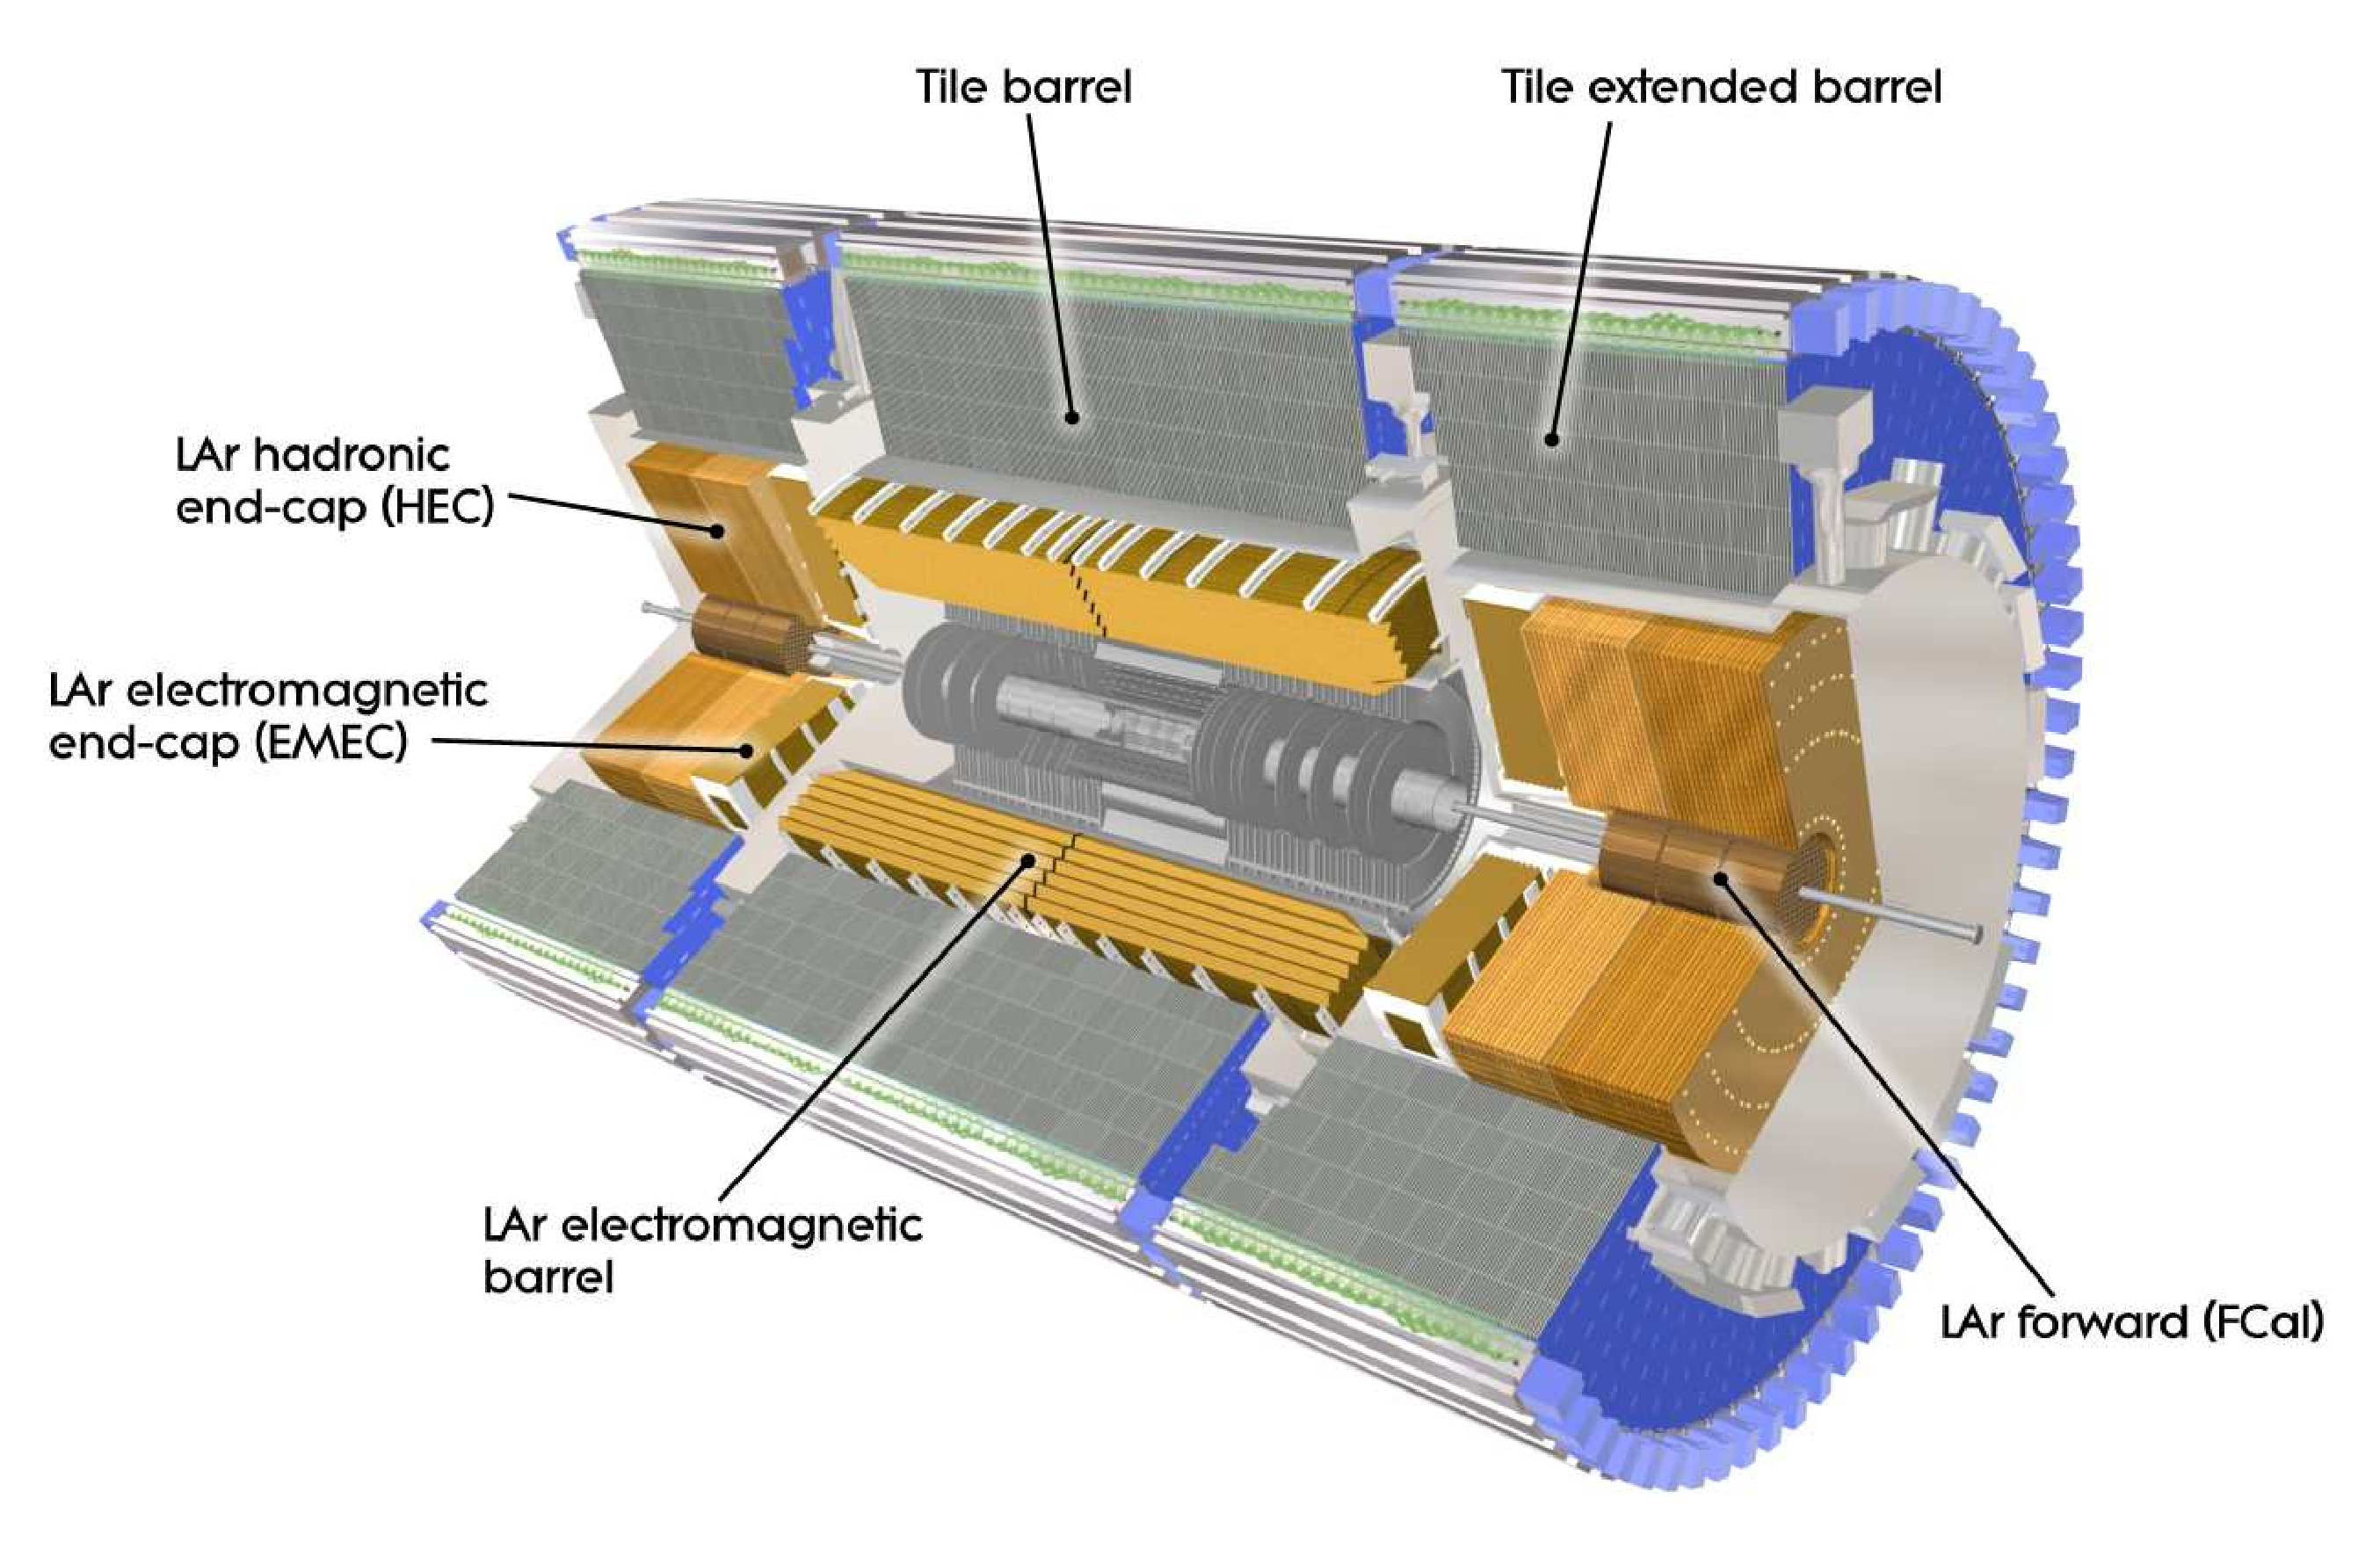
\includegraphics[width=\fullfig]{figures/calo_overview.pdf}
\caption{}
\label{fig:calo_overview}
\end{figure}

% This seems unnecessary, I will come back and add it if anyone asks for it.
%\begin{table}[hbtp]
%\begin{tabular}{lclll}
%\hline
%Component & Layers & Coverage & Granularity & Depth \\
%\hline
%\multicolumn{5}{c}{\ac{EM} Barrel Calorimeter}\\
%Layer 1 & 1 & $|\eta| < 1.475$ & 0.003 x 0.1 & 4.3 $X_0$ \\
%Layer 2 & 1 & $|\eta| < 1.475$ & 0.025 x 0.025 & 16 $X_0$ \\
%Layer 3 & 1 & $|\eta| < 1.475$ & 0.05 x 0.025 & 2 $X_0$ \\
%\multicolumn{5}{c}{\ac{EM} Endcap Calorimeter}\\
%Layer 1 & 1 & $1.375 < |\eta| < 3.2$ & 0.003 x 0.1 & 4.0 $X_0$ \\
%Layer 2 & 1 & $1.375 < |\eta| < 3.2$ & 0.025 x 0.025 & 20 $X_0$ \\
%Layer 3 & 1 & $1.5 < |\eta| < 2.5$ & 0.05 x 0.025 & 2 $X_0$ \\
%\multicolumn{5}{c}{Hadronic Tile Calorimeter}\\
%\multicolumn{5}{c}{EM Barrel Calorimeter}\\
%\multicolumn{5}{c}{EM Barrel Calorimeter}\\
%\hline
%\end{tabular}
%\caption{The granularity is measured in units of $\Delta\eta x \Delta\phi$.}
%\end{table}

The calorimeters are designed to absorb and measure the energy carried by a particle, and completely stop the particle's propagation in the process.
This requires a significant amount of material to provide interactions.
These interactions then produce secondary particles, which can produce tertiary particles in turn, and thus form a cascade of particles called an \ac{EM} or hadronic shower, depending on the governing mechanism.
Electromagnetic and hadronic showers have very different properties and require different technologies to measure them accurately.
All of the calorimeters in the ATLAS calorimeter system are sampling calorimeters: they use alternating layers of absorbing and active material.
The dense absorbing layers initiate the showers while the active layers measure the energy of the produced particles.
A fraction of the energy is lost in the inactive layers, so the energy measurement from the active layers has to be corrected to estimate the actual energy of the particle.

The \ac{EM} calorimeter provides around 20 radiation lengths ($X_0$) while the hadronic calorimeter provides around 10 interaction lengths ($\lambda$). 
As mentioned previously, radiation lengths measure the distance over which an electromagnetically interacting particle loses a characteristic fraction of its energy.
Interaction lengths, on the other hand, measure the mean distance traveled by a hadronic particle before undergoing a nuclear interaction~\cite{pdg}.
Figure~\ref{fig:calo_interactionlengths} show the radiation lengths in the layers of the \ac{EM} calorimeter in the barrel region as well as the interaction lengths for all calorimeters.


\begin{figure}[hbtp]
\subfloat[]{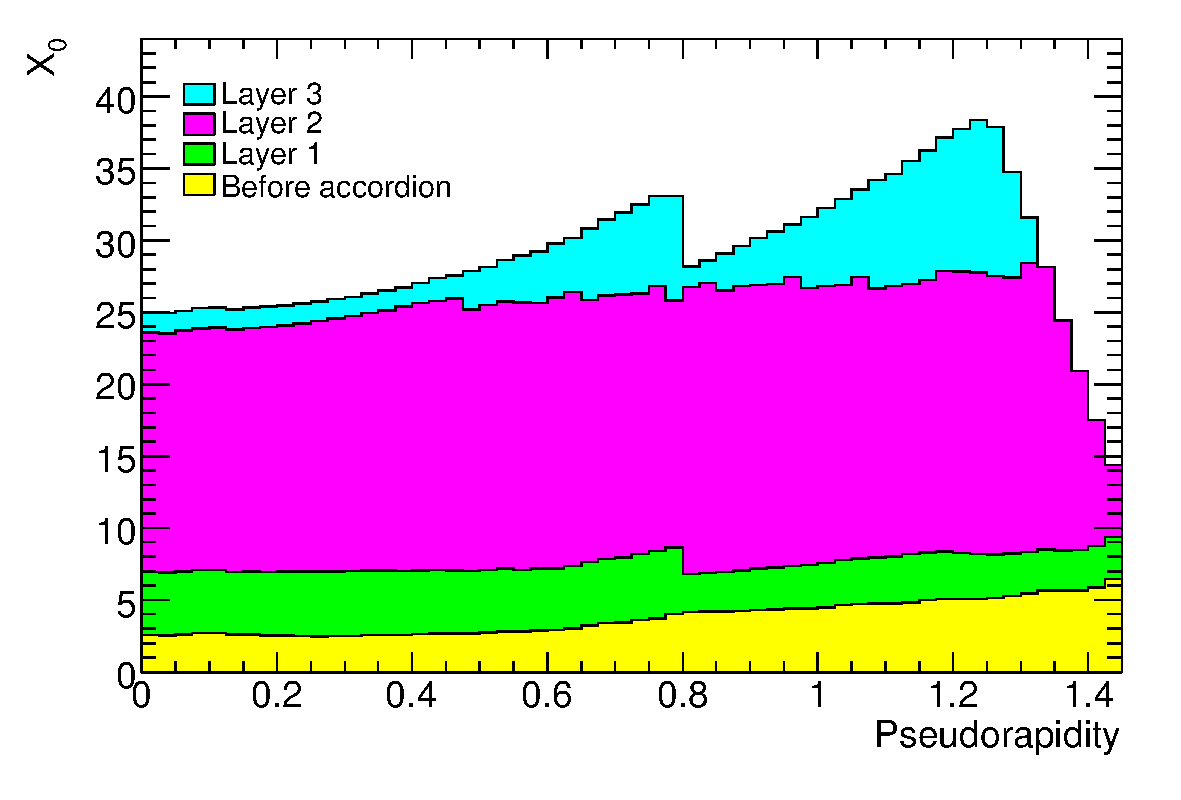
\includegraphics[width=\halffig]{figures/calo_radiationlengths.pdf}}
\subfloat[]{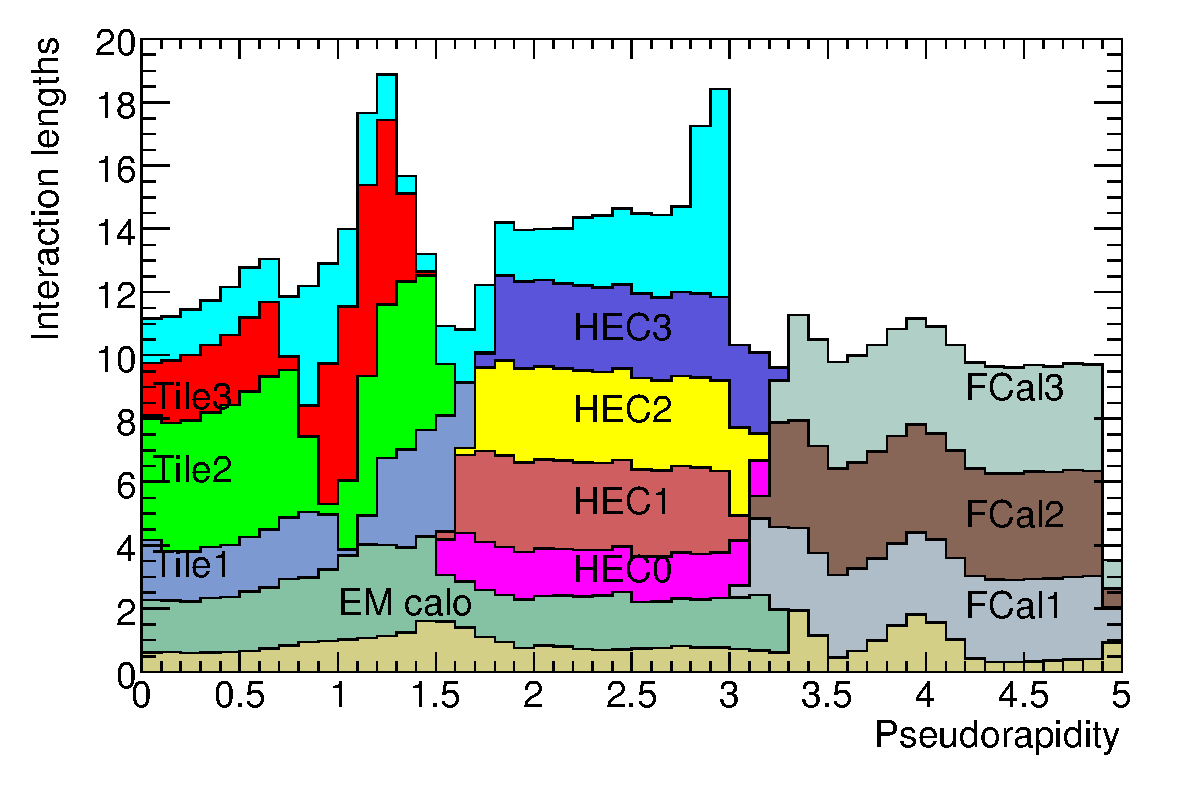
\includegraphics[width=\halffig]{figures/calo_interactionlengths.pdf}}
\caption{The depth of (a) the electromagnetic barrel calorimeter in radiation lengths and of (b) all calorimeters in interaction lengths as a function of pseudorapidity.}
\label{fig:calo_interactionlengths}
\end{figure}

\subsection{Electromagnetic Calorimeter}

The electromagnetic calorimeters use alternating layers of \acl{LAr} and lead in an accordion shape. 
The accordion shape provides complete coverage in the $\phi$ direction while also providing many alternating layers for the a particle to pass through.
The configuration is detailed in Figure~\ref{fig:calo_barrel_schematic}.
When an electron or a photon passes through the lead, it produces an electromagnetic shower.
The particles produced in those showers then pass into and ionize the \acl{LAr}; the ions produced can then be collected by an electrode in the \acl{LAr} layer to provide the actual energy measurement.

\begin{figure}[hbtp]
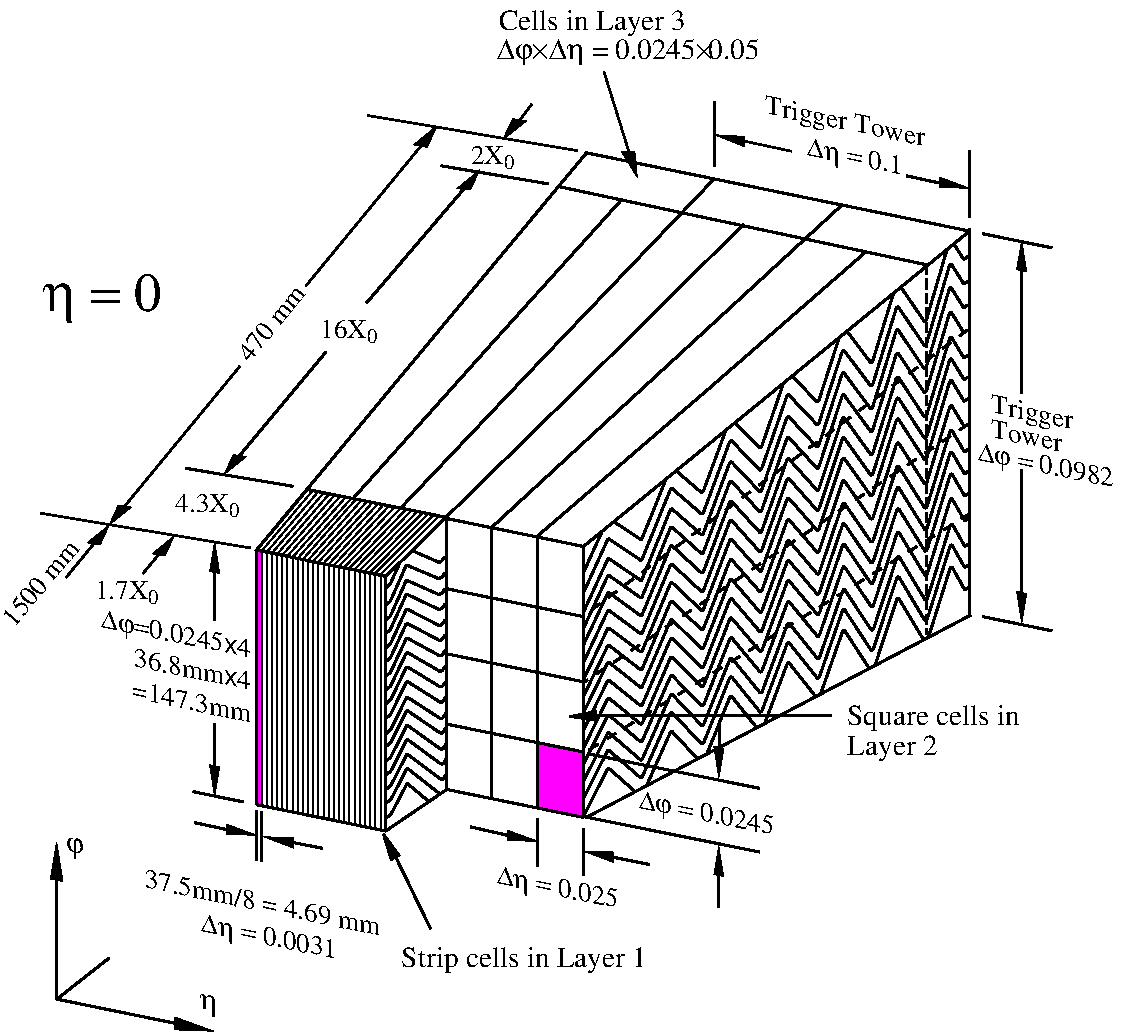
\includegraphics[width=\fullfig]{figures/calo_barrel_schematic.pdf}
\caption{A schematic of the \ac{LAr} calorimeter in the barrel region, highlighting the accordion structure.}
\label{fig:calo_barrel_schematic}
\end{figure}

The barrel region is covered by a presampler and three separate sampling layers with decreasing segmentation.
The presampler is a thin layer of \acl{LAr} which measures the energy of any electromagnetic showers which are initiated before the particle reaches the calorimeter due to interactions with the detector material.
The first layer is the strip layer, which has fine segmentation in $\eta$ to enhance the identification of shower shapes and to provide a precise $\eta$ measurement for reconstructing photons and electrons.
The strip layer has only 4 radiation lengths worth of material, and has a segmentation of $\Delta\eta = 0.003$ and $\Delta\phi = 0.1$. 
The second layer is also finely segmented, with a segmentation of $\Delta\eta = 0.025$ and $\Delta\phi = 0.025$, and a thickness of 16 $X_0$.
This layer is designed to contain an electromagnetic shower and to measure the majority of the energy for photons and electrons.
The third layer is only 2 $X_0$ thick and measures the energy of electromagnetic showers which leak out of the second layer, and helps to separate electromagnetic showers from hadronic showers. 
The structure of the \ac{LAr} endcap calorimeter is similar except that the layers are arranged parallel to the beampipe to measure energy deposits from high $\eta$ particles.

%\begin{figure}[hbtp]
%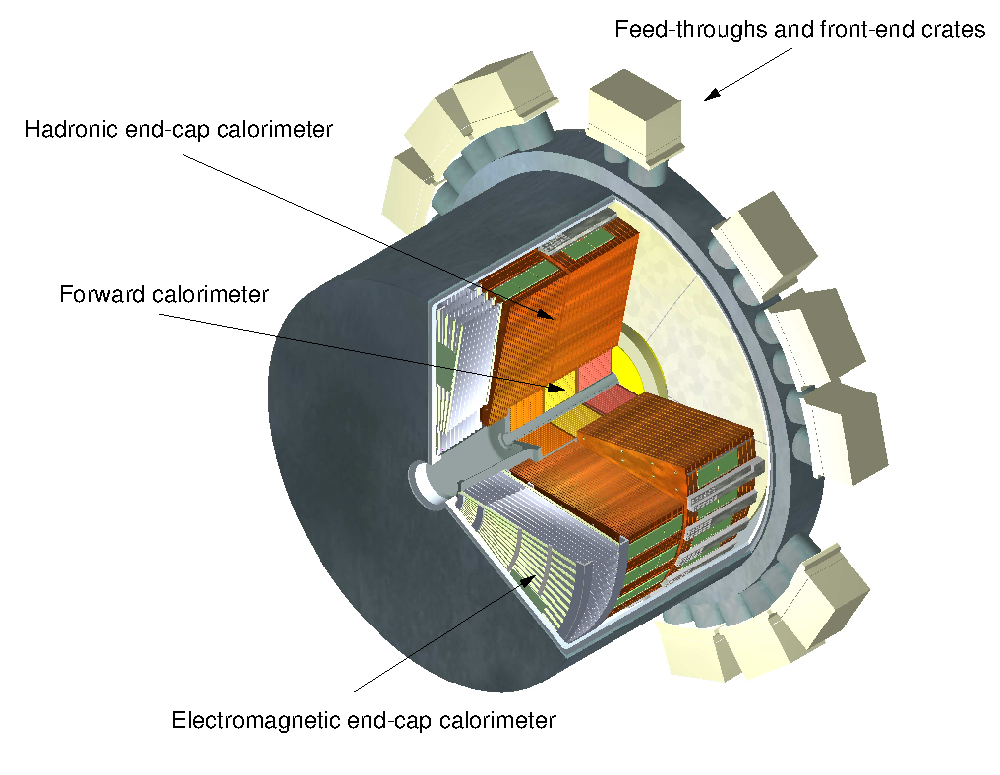
\includegraphics[width=\fullfig]{figures/calo_endcap_overview.pdf}
%\caption{}
%\label{fig:calo_endcap_overview}
%\end{figure}

\subsection{Hadronic Calorimeters}

The hadronic calorimeters use a few different technologies to satisfy the resolution demands in the different areas of the detector, and together they cover the region $|\eta| < 2.7$.
In the barrel region, for $|\eta| < 1.7$, the hadronic calorimeters are constructed of alternating tiles of steel and plastic scintillator. 
Like in the electromagnetic calorimeter, the dense layer initiates a shower (in this case the dense layer is the steel and the shower is hadronic) of particles which pass into and ionize the following layer.
The ionization in the plastic scintillator instead produces a light signal proportional to the amount of ionization produced by the shower, and this signal is measured using photomultipliers and provides the actual energy measurement.
The construction of a tile in the calorimeter is shown Figure~\ref{fig:hadronic_tile}, which highlights the alternating layers of steel and scintillator.

\begin{figure}[hbtp]
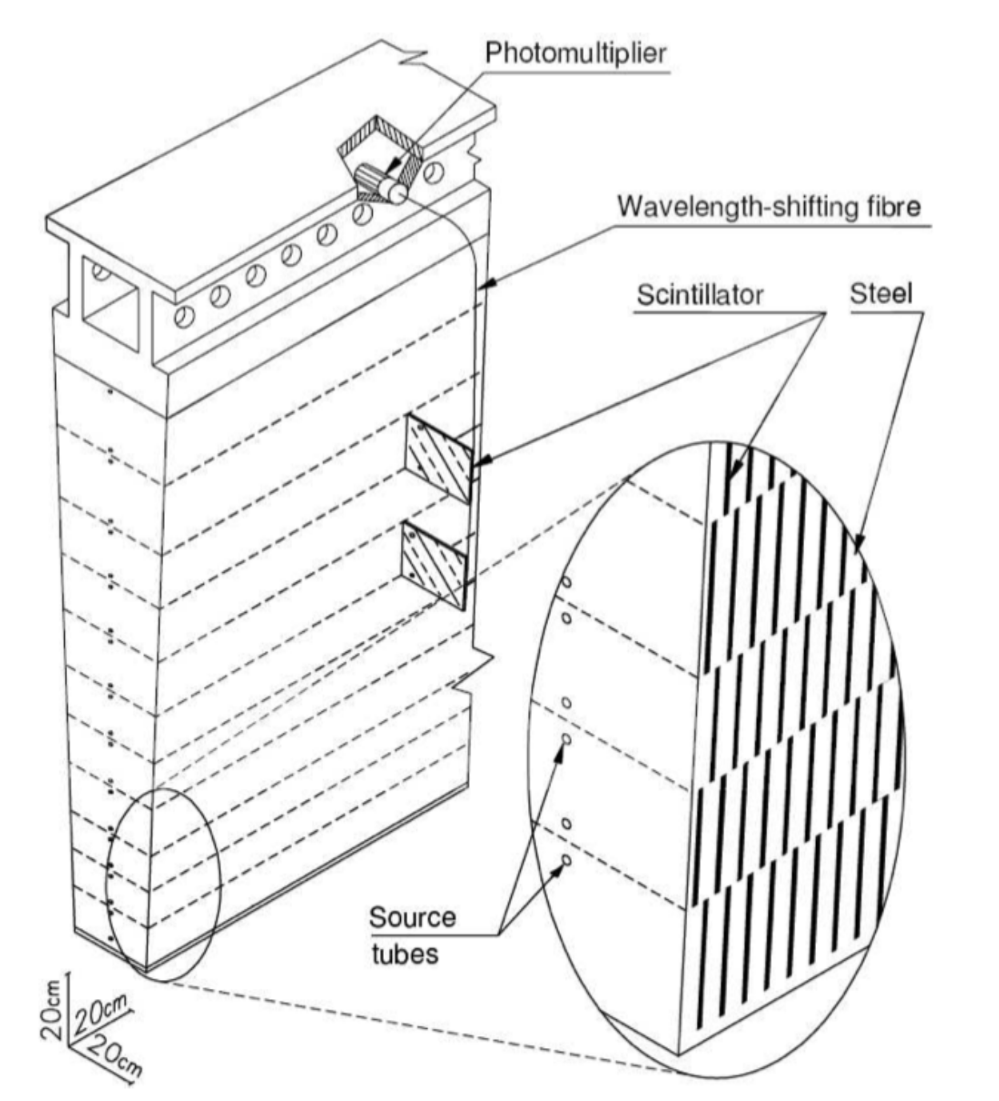
\includegraphics[width=\fullfig]{figures/hadronic_tile.png}
\caption{A schematic of a hadronic tile module which shows the alternating layers of steel and plastic scintillator.}
\label{fig:hadronic_tile}
\end{figure}

This tile calorimeter, as well as the remaining hadronic calorimeters, have a much coarser granularity than the electromagnetic calorimeters.
The high granularity is not needed for an accurate energy measurement, and the hadronic calorimeters are not designed to distinguish particle types like the electromagnetic calorimeters.
The tile granularity is approximately $\Delta\eta = 0.1$ and $\Delta\phi = 0.1$, and the segmentation in depth and $\eta$ is shown in Figure~\ref{fig:tile_segmentation}.

\begin{figure}[hbtp]
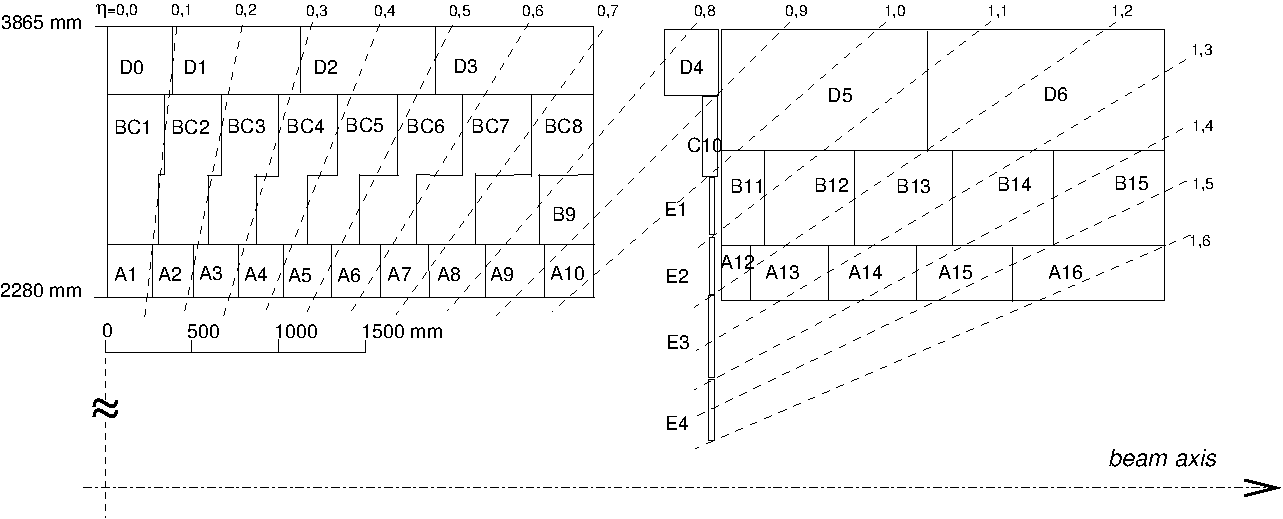
\includegraphics[width=\fullfig]{figures/tile_segmentation.pdf}
\caption{The segmentation in depth and $\eta$ of the tile-calorimeter modules in the central (left) and extended (right) barrels.}
\label{fig:tile_segmentation}
\end{figure}

The remaining hadronic calorimeters all use the same alternating, sampling structure but with different active and inactive materials.
The hadronic endcap calorimeter covers the range of $1.5 < |\eta| < 3.2$ and uses an inactive layer of copper and an active layer of \acl{LAr}.
The forward calorimeter covers the range of $3.1 < |\eta| < 4.9$ and uses a dense matrix of copper and tungsten filled with \acl{LAr}. 
Particles propagating through the sampling layers ionize the \acl{LAr}, and the ionization is collected at an electrode to provide a signal.

% ----------------------------------------

\section{Muon Spectrometer}

Among \ac{SM} particles, only muons and neutrinos consistently pass through the calorimeters.
Because the neutrinos are also electrically neutral, there is no feasible option to measure them directly in ATLAS.
The muons, on the other hand, are charged and are thus already measured as a track in the inner detector.
The muon spectrometer provides a way to consistently identify muon tracks and also a way to provide an additional measurement of their momentum.

The muon spectrometer contains four subdetectors that cover the barrel and endcap regions.
In the barrel region, the muon spectrometer uses a combination of \acp{RPC} and \acp{MDT} to provide both a coarse, fast measurement for triggering and a precise momentum measurement for offline event reconstruction.
Similarly, in the endcap region, the \acp{TGC}, \acp{MDT}, and \acp{CSC} allow for both triggering and precise measurements.
The \acp{CSC} are used only in the innermost layer of the endcap region between $2.0 < |\eta| < 2.7$ where the particle flux is too large for the \acp{MDT} to provide accurate measurements.
The overall layout of the muon systems are shown in the cut-away diagram in Figure~\ref{fig:muon_overview}, and Figure~\ref{fig:muon_side_schematic} shows a precise schematic of the layout of each of the detecting elements.
The geometric arrangement shown provides consistent coverage for muons produced up to $|\eta| < 2.7$, and takes full advantage of the bending of the muons in the toroidal magnetic field, described in Section~\ref{sec:magnetic_field}, to measure their momentum.
Figure~\ref{fig:muon_barrel_schematic} shows a cross-section of the arrangement of the muon spectrometer in the barrel; the layers are divided into eight small and eight large chambers that are overlapped to provide complete coverage in $\phi$. 


\begin{figure}[hbtp]
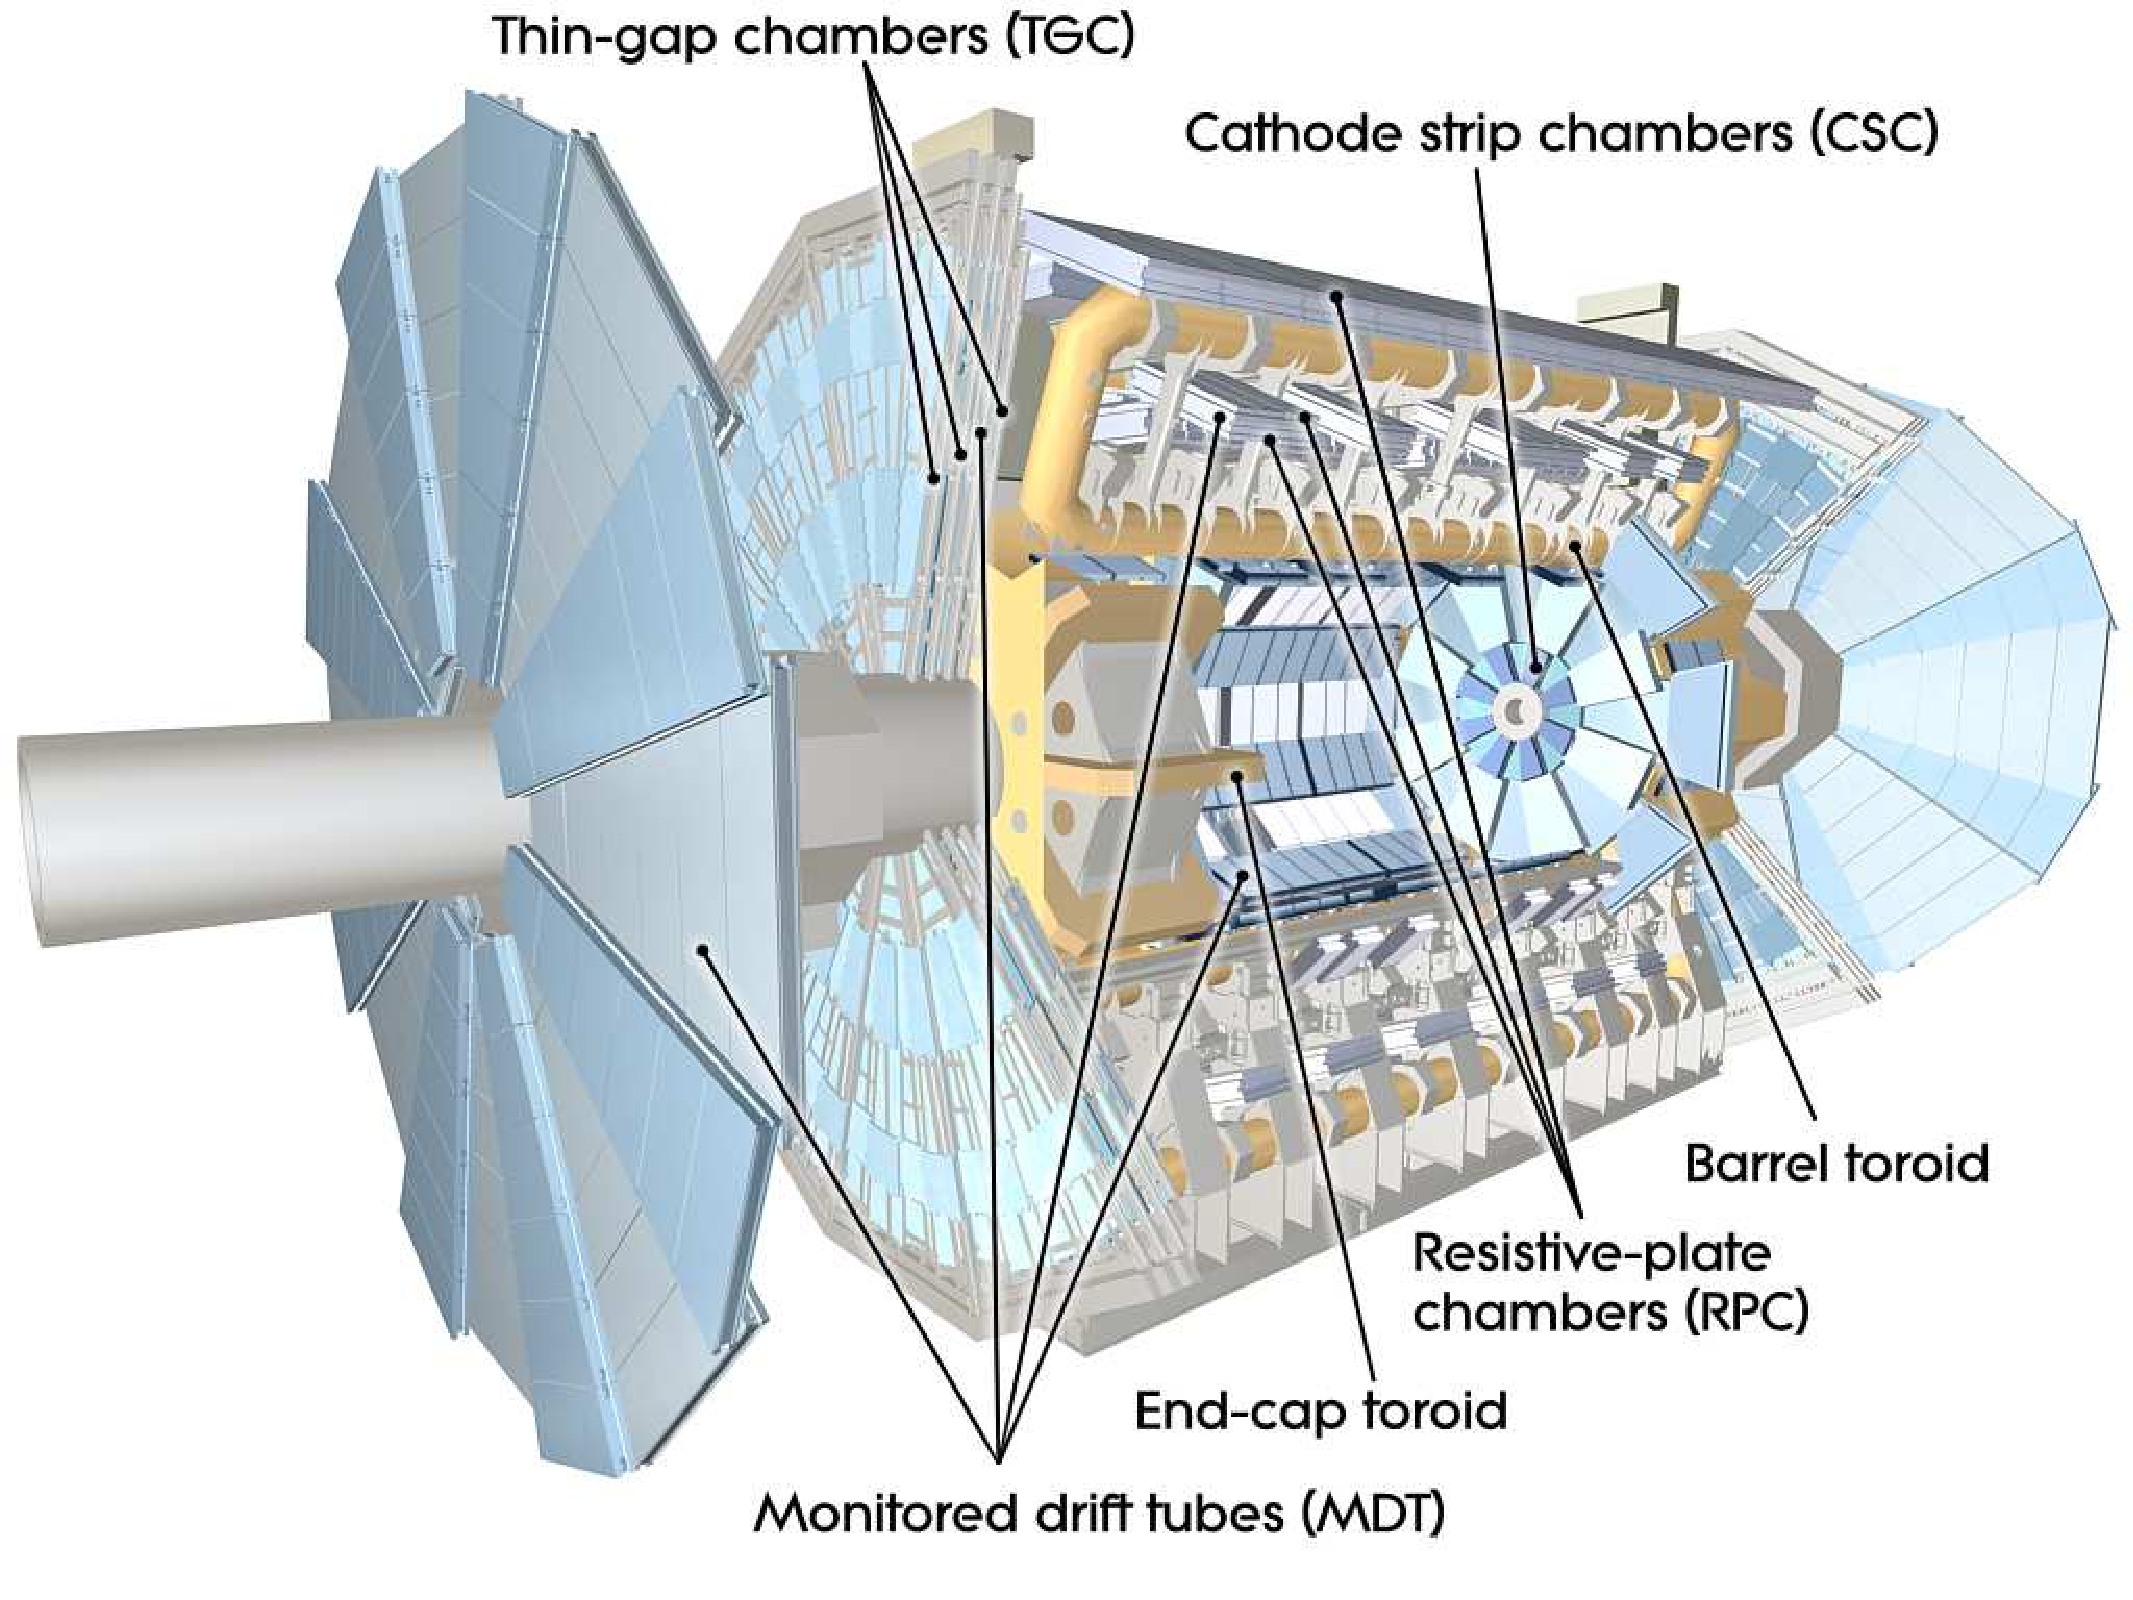
\includegraphics[width=\fullfig]{figures/muon_overview.pdf}
\caption{A cut-away diagram of the muon systems on ATLAS.}
\label{fig:muon_overview}
\end{figure}

\begin{figure}[hbtp]
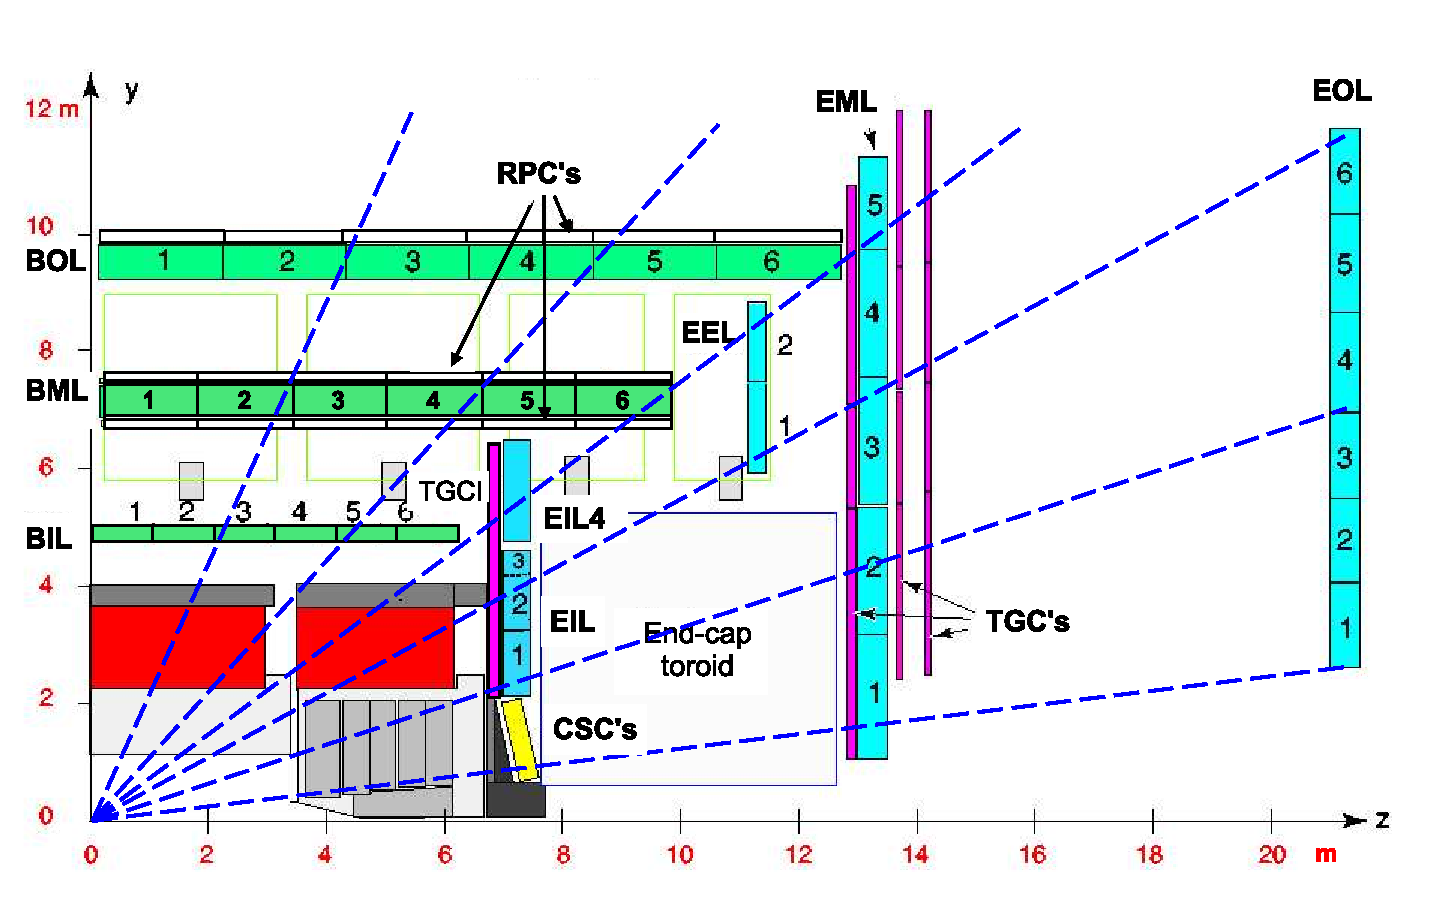
\includegraphics[width=\fullfig]{figures/muon_side_schematic.pdf}
\caption{A quarter view of the muon spectrometer which highlights the layout of each of the detecting elements. The BOL, BML, BIL, EOL, EML, and EIL are all \ac{MDT} elements, where the acronyms encode their positions.}
\label{fig:muon_side_schematic}
\end{figure}

\begin{figure}[hbtp]
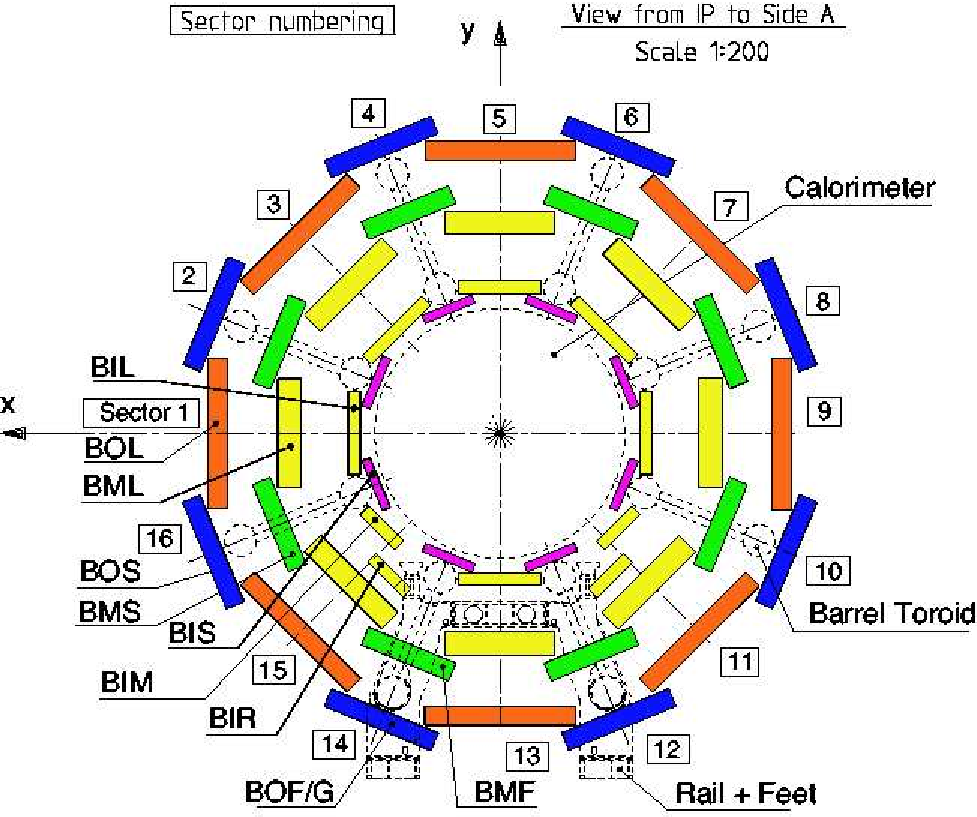
\includegraphics[width=\fullfig]{figures/muon_barrel_schematic.pdf}
\caption{A schematic of the cross-section of the muon spectrometer in the barrel region.}
\label{fig:muon_barrel_schematic}
\end{figure}


\subsection{\acl{MDT}}
\label{sec:mdt}
The momentum measurements in the barrel region are provided by three consecutive layers of \ac{MDT} elements, located at approximately 5 m, 7 m, and 9 m from the interaction point.
Each of these layers is a composite of two multilayers of drift tubes: two layers of three to four layers of tubes, as shown in Figure~\ref{fig:mdt_schematic}.
These aluminum tubes are 3 cm in diameter, with lengths between 0.9 and 6.2 m, and are filled with a mixture of ArCO\tsub{2} kept at 3 bar absolute pressure.
A central tungsten-rhenium wire with a diameter of 50 \um runs along the length of the tube, and is kept at a potential of 3080 V.

\begin{figure}[hbtp]
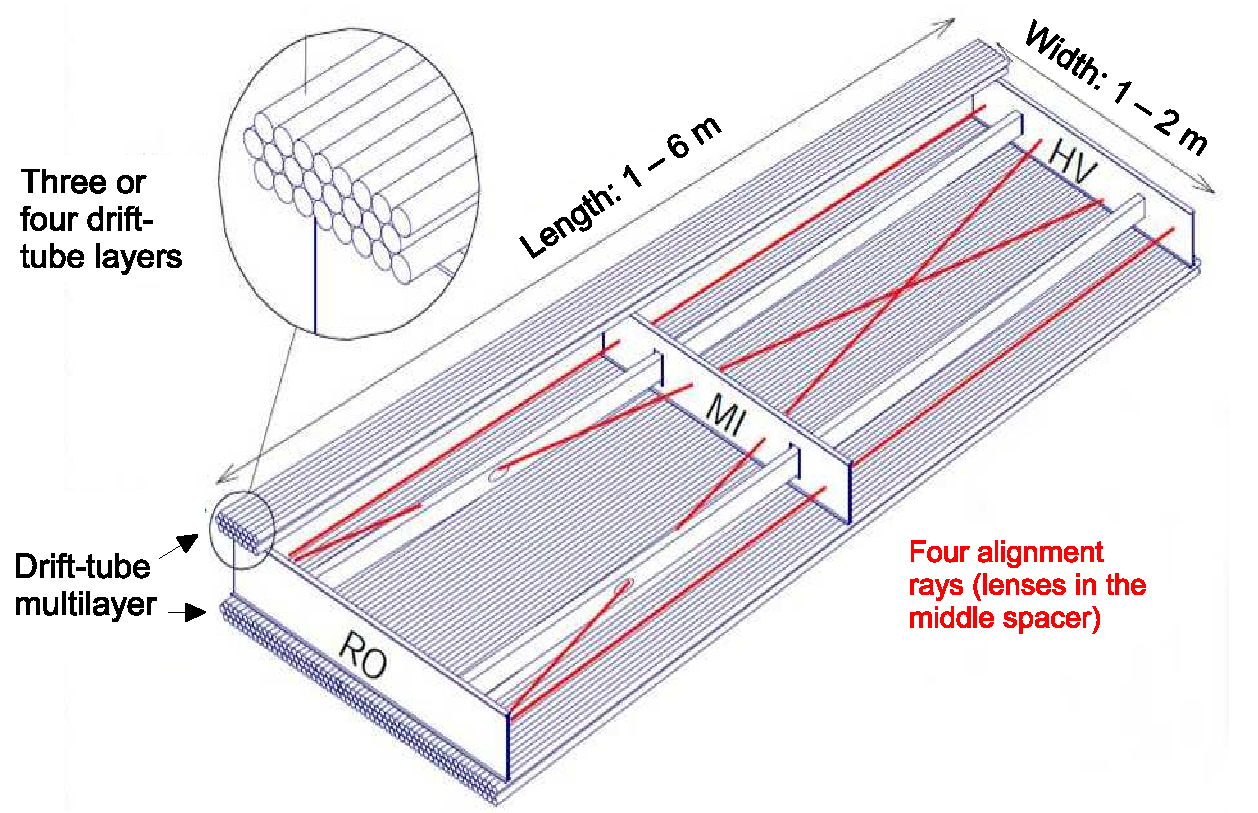
\includegraphics[width=\fullfig]{figures/mdt_schematic.pdf}
\caption{A schematic of a single \ac{MDT} chamber, which shows the multilayers of drift tubes as well as the alignment system.}
\label{fig:mdt_schematic}
\end{figure}

A muon traversing these tubes ionizes the gas, and the ionization electrons then drift in the electric field toward the central wire.
Close to the wire, the electric field is strong enough to cause the original ionization electrons to ionize additional electrons, producing an avalanche that can be measured as a current along the wire. 
The time of arrival of that current depends on how far the muon entered from the wire, and can be used to achieve a position resolution of 80 \um in an individual tube.
The combination of the measurements in the consecutive layers of tubes improves this position resolution to 35 \um transverse to the tubes, with a resolution of 1 m along the tube direction.

To achieve a good resolution over the entire length of a muon track, the relative positions of the tubes of the muon spectrometer must be known to an accuracy of 30\um. 
This is achieved by an optical laser alignment system placed in each of the individual chambers and throughout the cavern.
These monitor any changes in position or alignment due to effects like gravitational sag, temperature shifts, and the magnetic field.
The configuration of the alignment system within an individual chamber is also shown in Figure~\ref{fig:muon_barrel_schematic}.

\subsection{\acl{RPC}}

The \ac{RPC} is the provides a fast measurement of the $\phi$ position of muons for triggering in the barrel region.
The system has a lower spatial resolution than the \acp{MDT} but has a faster measurement with a time resolution of just a few tens of nanoseconds.
There are three \acp{RPC} layers in the muon spectrometer, two located on either side of the central \ac{MDT} layer and one located outside the final \ac{MDT} layer, as shown in Figure~\ref{fig:muon_side_schematic}.
The \acp{RPC} consist of two layers of parallel plates filled with a gas mixture of C\tsub{2}H\tsub{2}F\tsub{4}.
A muon passing through these systems ionizes the gas, like in the \ac{MDT}, which causes an avalanche of ionization electrons in the electric field maintained between the plates.
Metal strips on the outside of the chamber capacitively couple to the accumulated charge, and are read out to measure the $\eta$ and $\phi$ positions of the muon track. 

\subsection{\acl{CSC}}
The majority of the momentum measurements in the endcap region are provided by the \acp{MDT}.
In the most forward region of the muon spectrometer, between $2.0 < \eta < 2.7$, the particle flux is very high due to contributions from low energy photons and neutrons.
The \ac{MDT} can only sustain a hit rate of approximately 150 Hz/cm\tsup{2} because of limitations in the drift times of the gas and the capacity of the readout electronics. 
The \acp{CSC} were designed to handle higher hit rates, up to 1000 Hz/cm\tsup{2}, and provide the necessary coverage in that high flux region.

The \ac{CSC} consists of several multiwire proportional chambers, where the wires are oriented in the radial direction out from the beampipe.
There are eight large and eight small chambers, arranged to partially overlap in the $\phi$ direction, as shown in Figure~\ref{fig:csc_schematic}.
Like in the \ac{MDT}, a muon traversing the system produces ionization in the gas; here, however, the ionization is collected on a number of wires.
These wires couple to cathodes on the chambers which are segmented into strips in two directions.
The relative amount of charge on each of the neighboring strips can be used to interpolate to the position of the muon in both $\eta$ and $\phi$. 

\begin{figure}[hbtp]
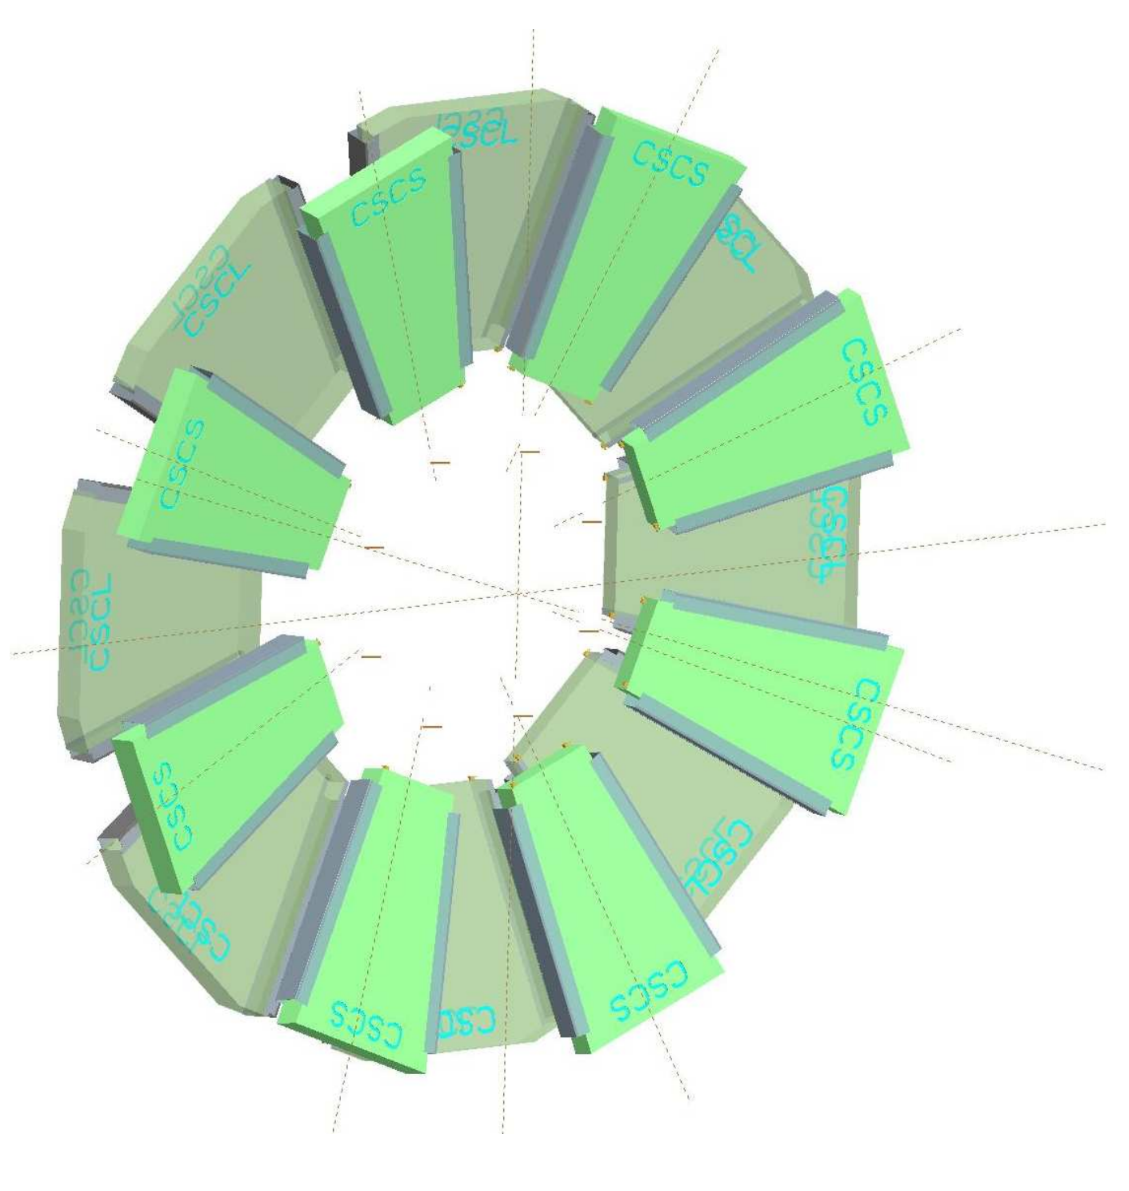
\includegraphics[width=\fullfig]{figures/csc_schematic.png}
\caption{A schematic of the \ac{CSC} endcap, showing the overlapping arrangement of the eight large and eight small chambers.}
\label{fig:csc_schematic}
\end{figure}

\subsection{\acl{TGC}}
Like in the barrel region, a separate, fast detector is required to provide position measurements of muons for trigger in the endcap region.
This is provided by the \ac{TGC} which consists of seven layers in the middle station of the endcap, two doublet layers and one triplet layer, and a single doublet layer in the inner endcap station.
Figure~\ref{fig:tgc_schematic} shows the arrangement of the triple and doublet layers of the \acp{TGC}.

\begin{figure}[hbtp]
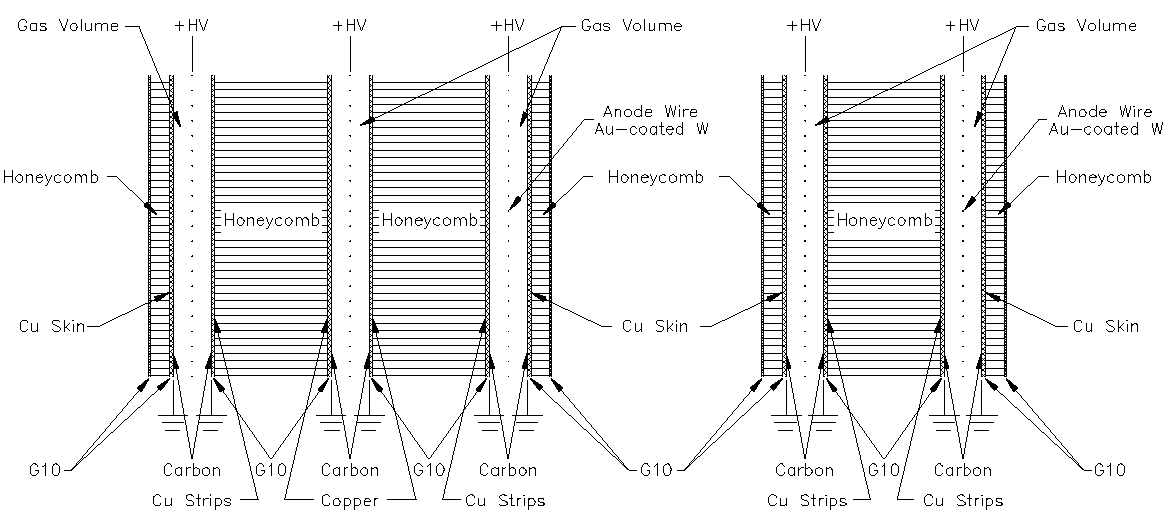
\includegraphics[width=\fullfig]{figures/tgc_schematic.pdf}
\caption{A schematic of the \ac{TGC} doublet and triplet layers.}
\label{fig:tgc_schematic}
\end{figure}

Like the \acp{CSC}, the \acp{TGC} are multiwire proportional chambers with a wire-to-cathode distance of 1.4 mm and a wire-to-wire distance of 1.8 mm.
Readout strips on the outside of the chambers run perpendicular to the wires, and couple to the charge collected on the wires to provide a position measurement in the $\eta$ direction.
The current induced on the wires is also readout to provide a position measurement in the $\phi$ direction.
The high electric field and small wire-to-wire distance give it the required good time resolution to be used for triggering events. 

% ----------------------------------------

\section{Trigger}
\label{sec:trigger}

It is not possible for the detector and the associated computing systems to record the 80 TB of data that the 40 MHz event rate produces every second.
Instead, a small fraction of these events are selected by the trigger system to be recorded and later analyzed.
Selecting interesting events at such a high rate poses a significant challenge for the both the detector design and the implementation of a trigger decision and data acquisition system.
The trigger must balance the time needed to decide to keep an event, to avoid losing information, with the filtering accuracy to consistently select a full menu of physics events that can be used for the wide array of searches and measurements targeted by ATLAS. 

The ATLAS trigger system, as of Run 2, consists of two levels of decision making. 
The first level, referred to as \ac{L1}, is hardware based and uses inputs from a subset of the detector elements to reduce the considered event rate from the original 40 MHz down to 100 kHz.
The 100 kHz rate is the maximal rate that the event information can be transferred from the detector.
The \ac{L1} trigger decisions must be made with 2.5 $\mu s$, or else the information stored from the event is still available to be read out to the next step.
The second, software-based level, referred to as the \ac{HLT}, makes the final decisions on which events to keep for analysis and selects a rate of around 1 kHz.
The collection of selection criteria used to make the \ac{L1} decisions feed into subsequent selection criteria in the \ac{HLT}, and the set of these combinations of \ac{L1} and \ac{HLT} criteria from the trigger menu which defines exactly what events are recorded on ATLAS.
A subset of the trigger menu used for 2015 data collection is shown in Table~\ref{tab:trigger_menu}, which summarizes the selection requirements at both levels and additionally shows the peak measured rates contributed by each.

\begin{table}[hbtp]
\centering
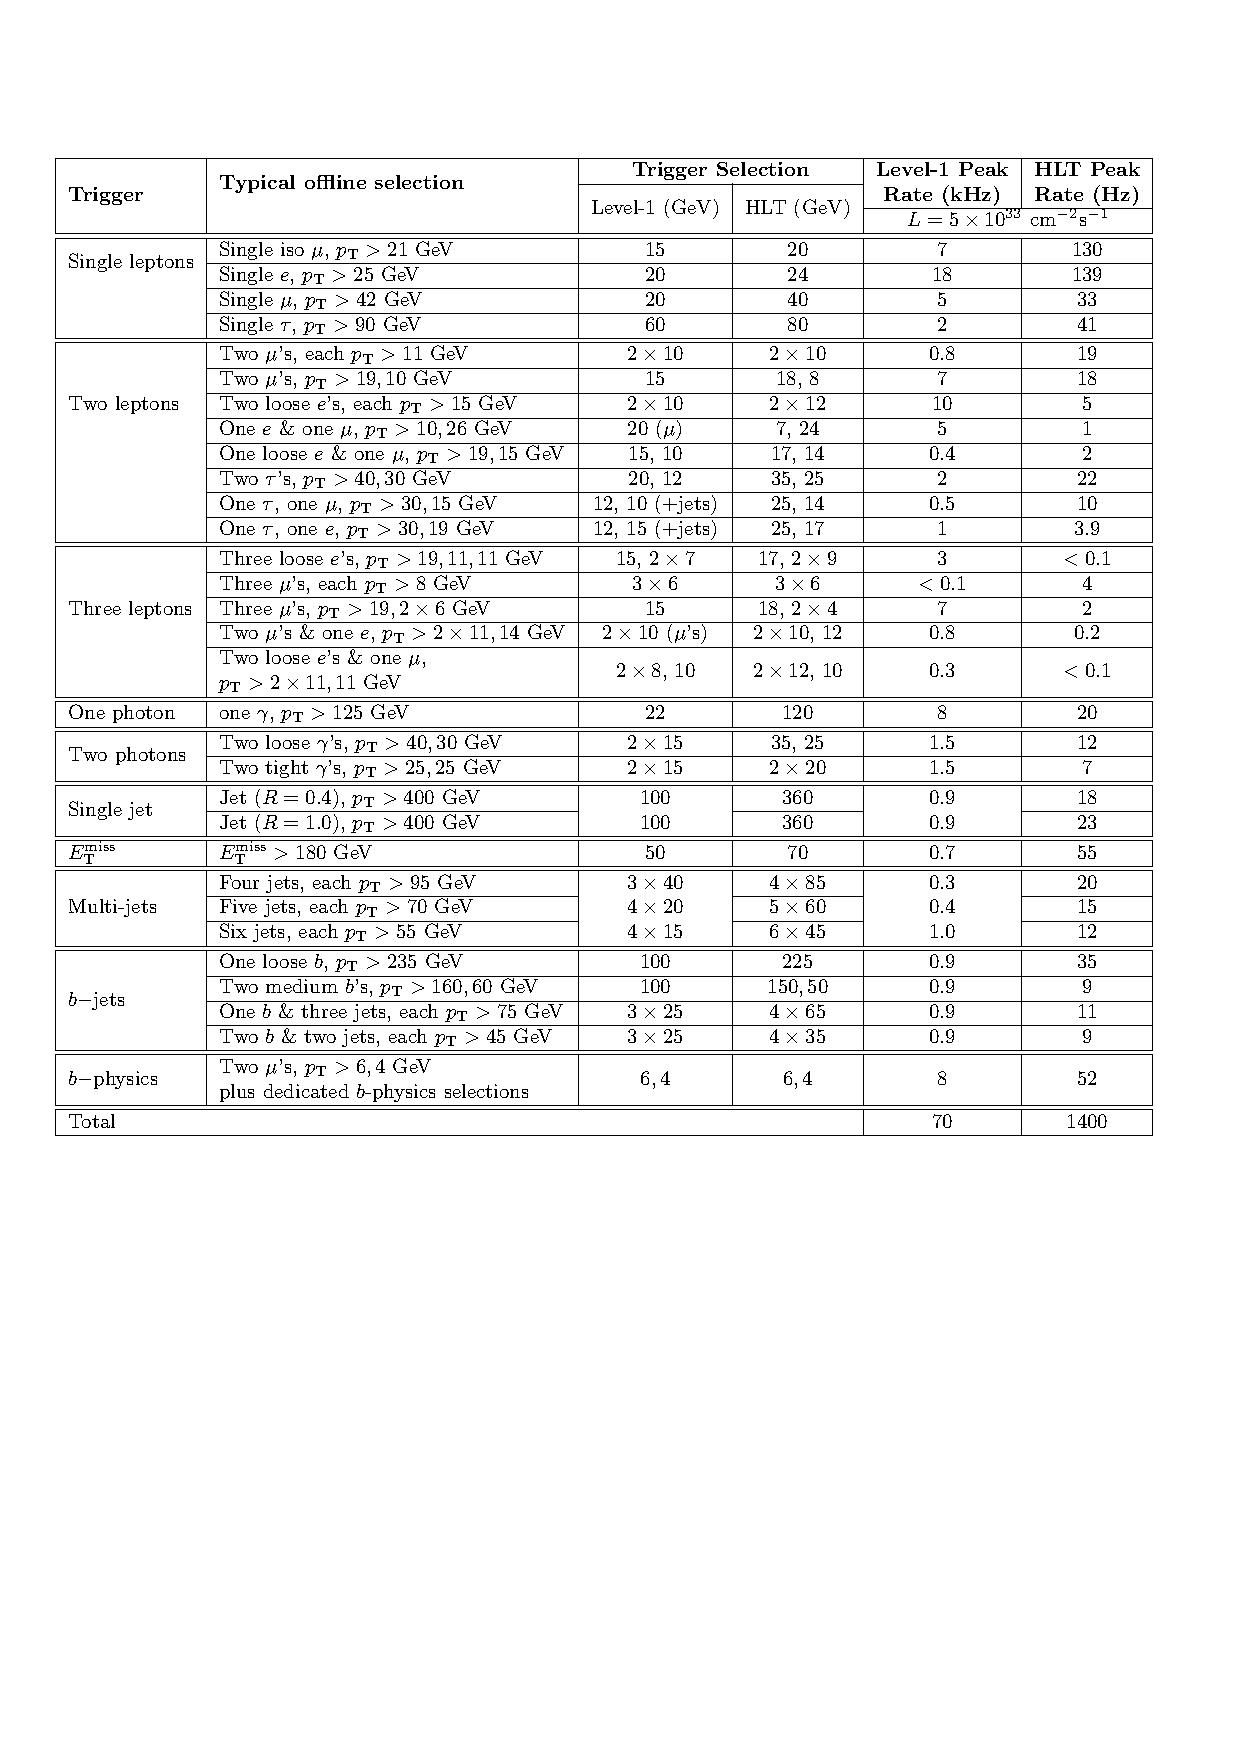
\includegraphics[width=\textwidth]{figures/trigger_menu.pdf}
\caption{A subset of the trigger menu for the 2015 data collection with $L = 5 x 10^{33}\lcms$. Both the \ac{L1} and \ac{HLT} selection requirements and their trigger rates are shown measured at the specified luminosity are shown. The typical offline selections represent a typical set of offline requirements imposed after the trigger in an analysis.}
\label{tab:trigger_menu}
\end{table}

At \ac{L1}, the trigger system uses information primarily from the calorimeters and muon spectrometer to select high \pt jets, electrons, photons, and muons. 
The electromagnetic calorimeter uses reduced granularity energy measurements as well as isolation requirements to select electrons and photons.
The hadronic calorimeter also uses a combination of reduced granularity energy measurements and isolation to select high momentum jets and hadronically decaying tau leptons. 
The calorimeters are also used to provide triggers based on missing energy: the coarse granularity energy measurements are used to calculate a directional sum of energies and to trigger on a significant imbalance.
The analysis discussed here uses the \met trigger shown in Table~\ref{tab:trigger_menu}, with a \ac{L1} rate of 0.7 kHz and an \ac{HLT} rate of 55 Hz.

Only the \acp{RPC} and \acp{TGC} muon subdetectors contribute to the decision at \ac{L1}, and are used to identify high momentum muons.
The contributions to the triggering rate of the various types of \ac{L1} triggers are shown in Figure~\ref{fig:trigger_l1rate}. 
The total rate is indicated in black and is lower than the sum of individual rates because their is significant overlap between different trigger channels. 
The majority of the rate comes from lepton and photon triggers.

\begin{figure}[hbtp]
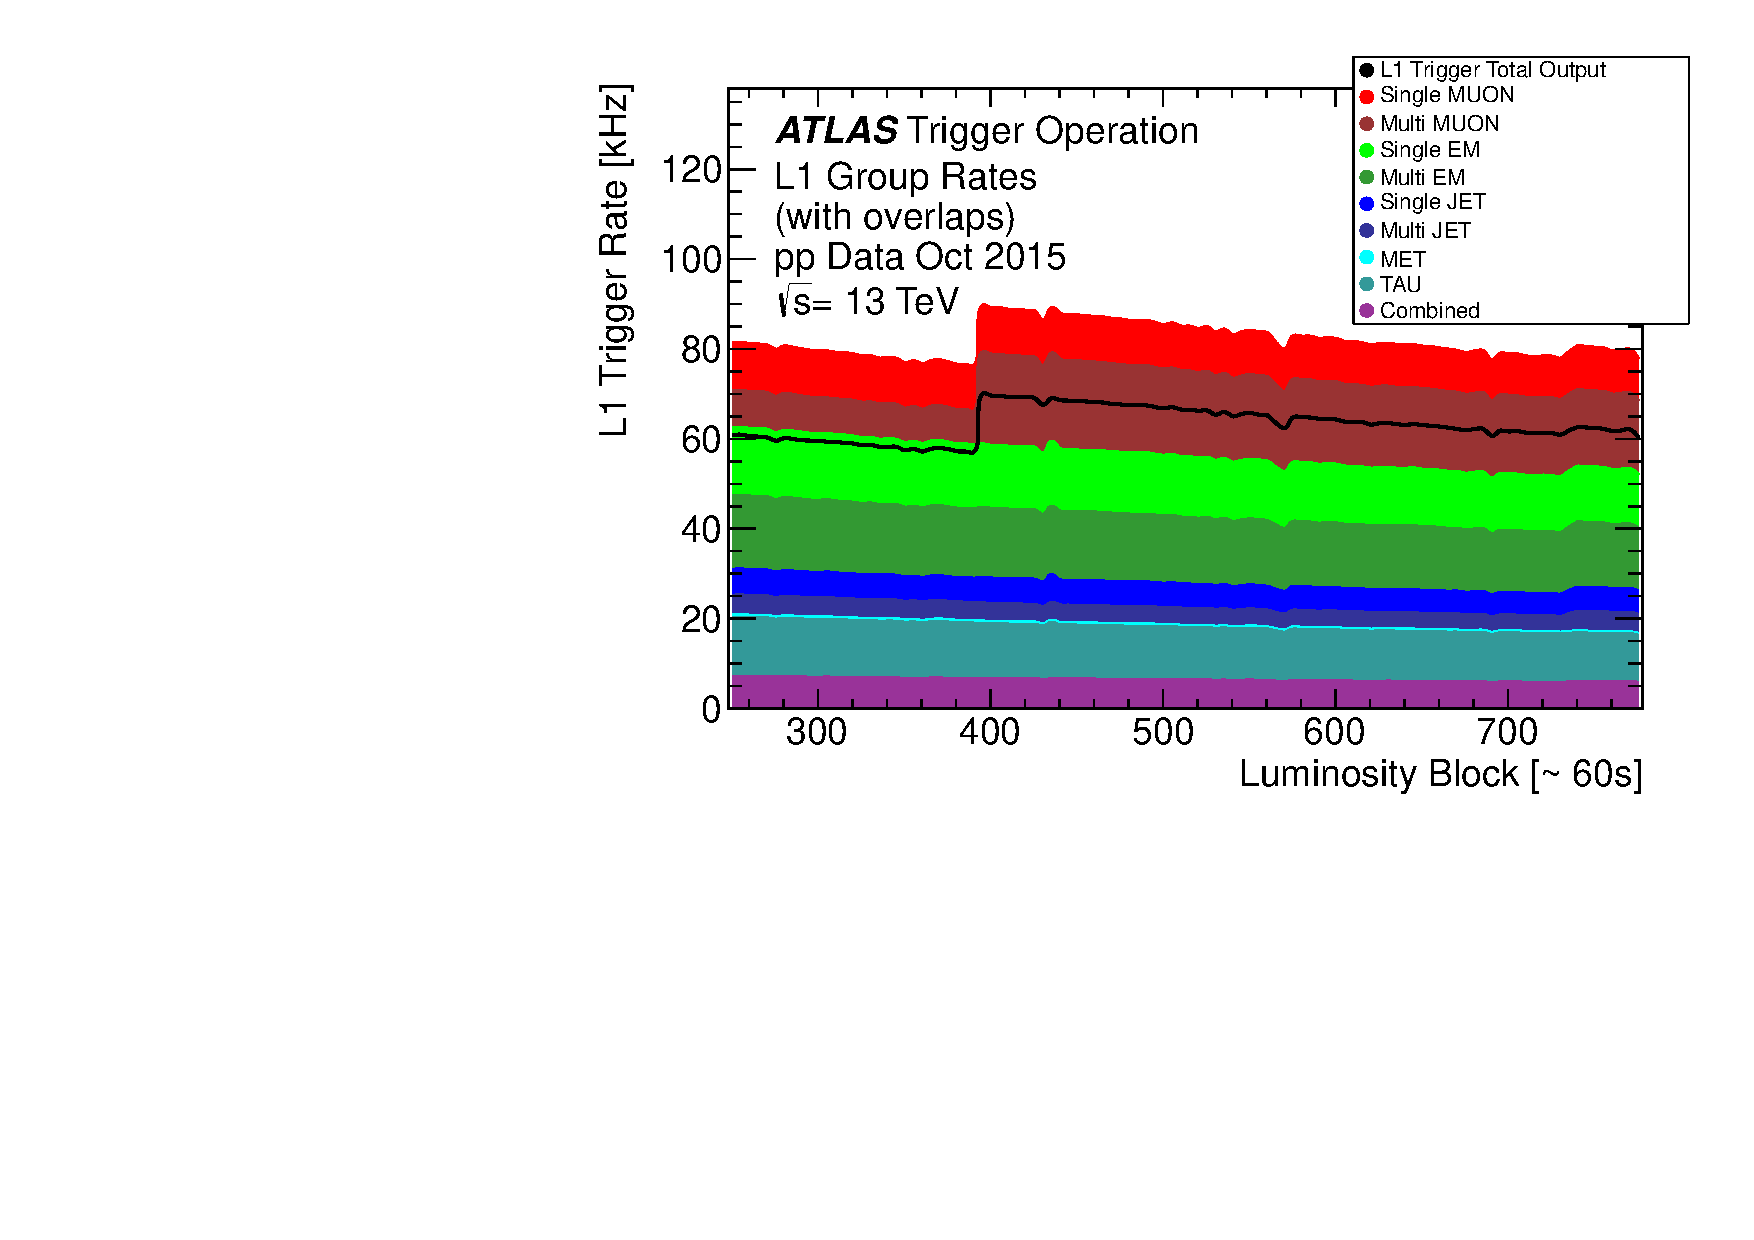
\includegraphics[width=\fullfig]{figures/trigger_l1rate.pdf}
\caption{The \ac{L1} Trigger rate broken down into the types of triggers as a function of the luminosity block for the 2015 data collection period.}
\label{fig:trigger_l1rate}
\end{figure}

After an event is chosen by the \ac{L1} trigger, the detector measurements from the bunch crossing which fired the trigger is read out from the front-end electronics and stored on read-out boards.
This inclusive information is necessary to make more the more precise event selections than is possible with the reduced information at \ac{L1}.
The \ac{HLT} then uses this information with software algorithms to decide whether or not to permanently record the event.
The \ac{L1} trigger also forwards which decision was made and \acp{RoI} to the \ac{HLT}, which allows the \ac{HLT} to focus on particular algorithms and particular sections of the detector to greatly improve the algorithmic selection speed.
The additional information available to the \ac{HLT} allows it to use full offline reconstruction algorithms (Chapter~\ref{ch:reconstruction}) to implement additional trigger targets, such as identified jets from the decays of b-hadrons.
The contributions to the triggering rate of the various types of \ac{HLT} triggers are shown in Figure~\ref{fig:trigger_hltrate}. 

\begin{figure}[hbtp]
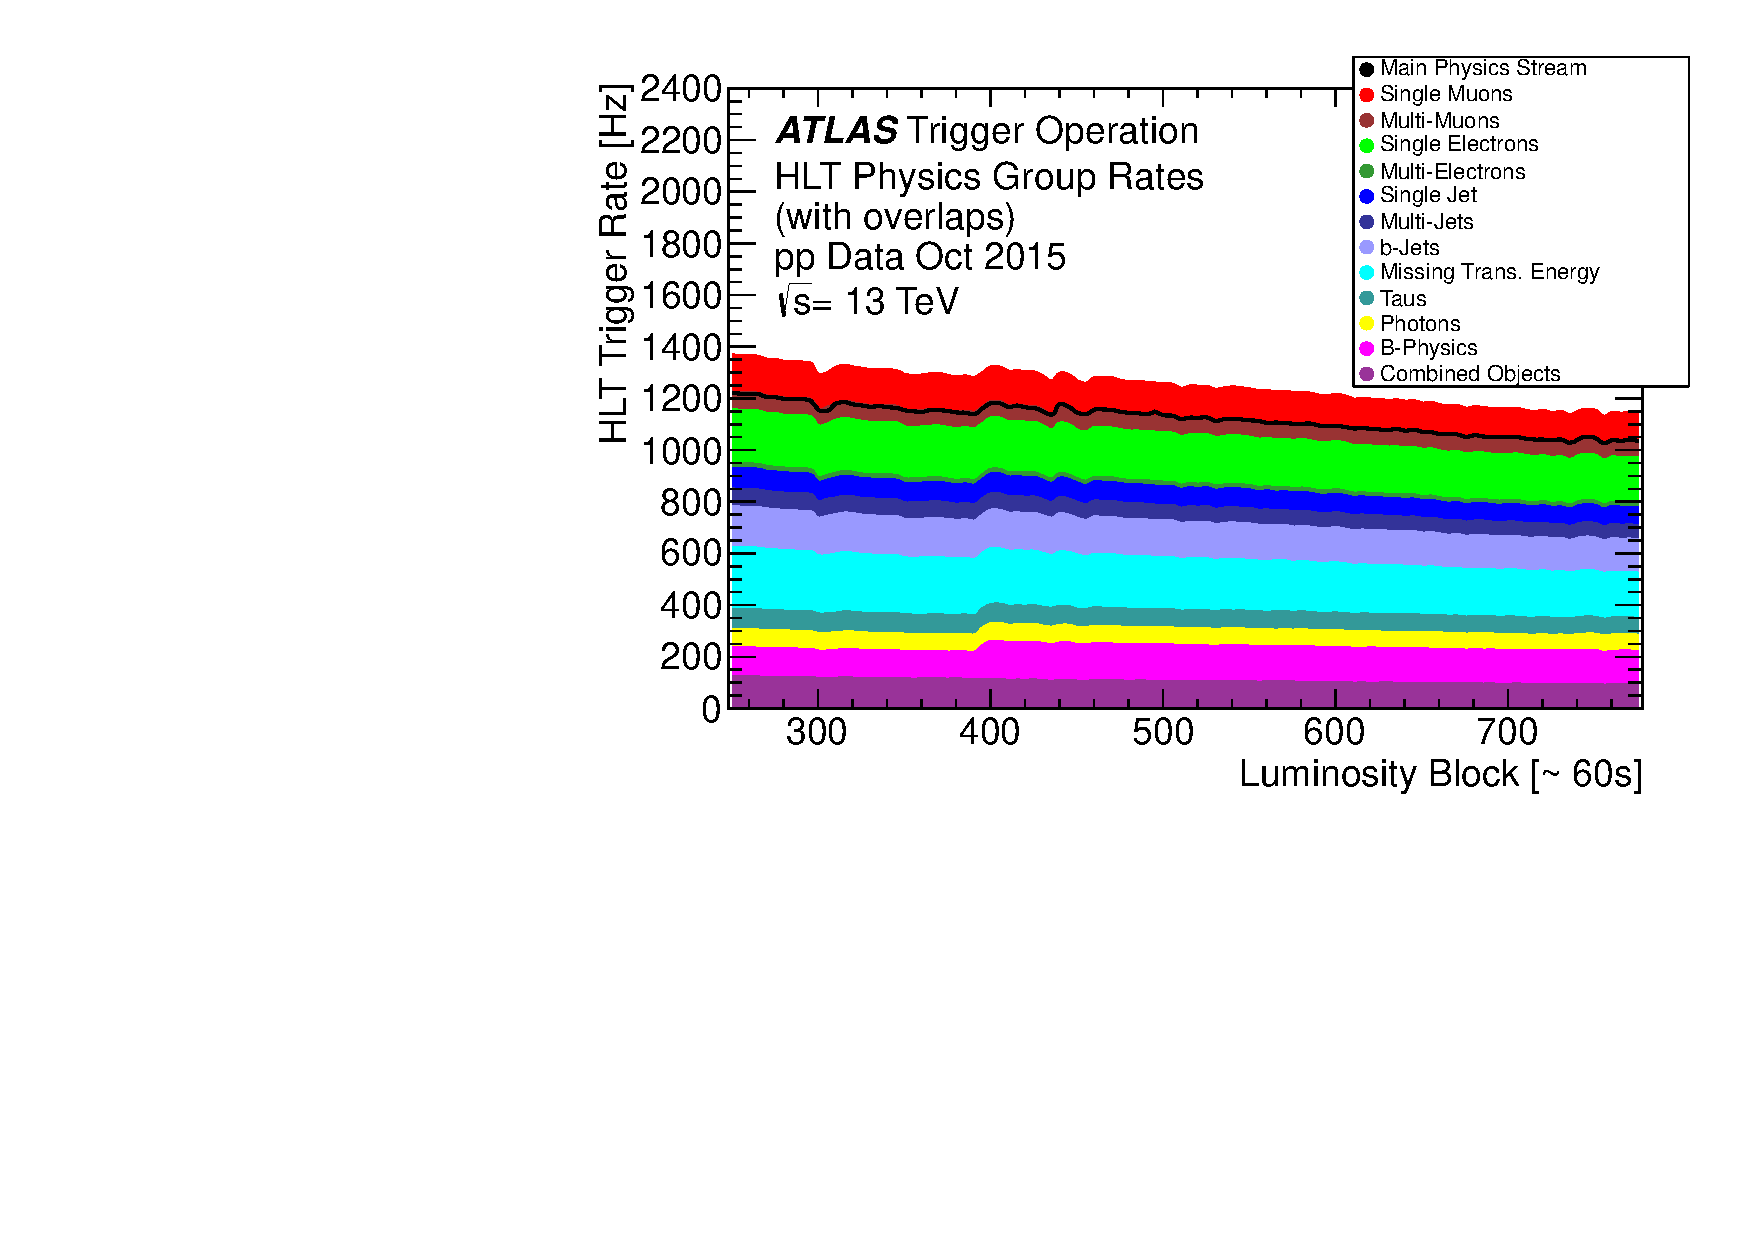
\includegraphics[width=\fullfig]{figures/trigger_hltrate.pdf}
\caption{The HLT Trigger rate broken down into the types of triggers as a function of the luminosity block for the 2015 data collection period.}
\label{fig:trigger_hltrate}
\end{figure}

% ----------------------------------------

\chapter{Event Reconstruction}

\label{ch:reconstruction}
% --------------------------------------------------------------------------------

The ATLAS experiment combines measurements in the subdetectors to form a cohesive picture of each physics event. 
The majority of particles that traverse the detector leave behind some combination of ionization hits in the tracking detectors or energy deposits in the calorimeters, and these measurements can be used to reconstruct physical quantities like the particle's energy, momentum, or trajectory.
Even the type of the particle can be distinguished by comparing the various ways that different species of stable particles interact with the subdetectors.
Reconstruction is the series of algorithms which take the electronic outputs of the detector and assigns them into individual physics objects.
The physics objects summarize the properties of particles produced by the collision or subsequent decays, either for individual isolated particles like leptons, or for a collection of the cascade of products produced in the decay of an energetic hadron, called a jet. 
These are the objects and quantities most often used in analysis to make measurements of \ac{SM} processes or to search for new physics.

% ----------------------------------------

\section{Charged Particles}
\label{sec:tracks}

As described in Section~\ref{sec:inner_detector}, charged particles that traverse the inner detector leave behind hits in the subdetectors.
Each of these hits translates into a position measurement along the trajectory of that particle, with position resolutions depending on the subdetector that provided the measurement. 
Track reconstruction uses these position measurements to collect hits in consecutive layers of the detector into a trajectory consistent with a particle curving in a magnetic field~\cite{newt, tracking_performance}.
This reconstructed trajectory is called a track.
The number of hits in the inner detector for each event makes a combinatorial method completely infeasible: the algorithms that form tracks must be significantly more intelligent so that event reconstruction does not exhaust computing resources.

The first and primary algorithm employed in track reconstruction is called the inside-out method, which begins with the assumption that the track originated from the interaction point.
Its purpose is to identify primary particles, those which originate in the proton-proton collisions and with a lifetime long enough to reach the inner detector.
Combinations of three hits are considered from measurements in the Pixel detector and the \ac{SCT}, and form the seed for a track. 
Specifically, the seeding algorithm looks for a seed using three pixel hits, two pixel hits and one \ac{SCT} hit, or three \ac{SCT} hits.
The seed is then extrapolated forwards and backwards into the Pixel and \ac{SCT} detectors depending on the seed location, and hits in each layer are considered to be added to the track using a combinatorial Kalman filter~\cite{tracking_performance}.
After all of the silicon layers have been considered, tracks are filtered to reduce ambiguities from other nearby tracks or from combinatorial coincidences.
Then the tracks are extended outwards into the \ac{TRT} in the same way.
The result of this clustering algorithm is a collection of hits identified to belong to a single track.
Once the hits are collected, a fitting algorithm calculates the track parameters which best model the locations of the hits and their resolutions.
The fitting uses five parameters, $(d_0, z_0, \phi, \theta, q/p)$, to specify a track in a perigee representation: $d_0$ and $z_0$ are the transverse and longitudinal impact parameters at the closest approach to the nominal beam axis, $\phi$ and $\theta$ are the usual angular coordinates, and $q/p$ is the charge divided by the curvature.
These parameters are illustrated in Figure~\ref{fig:perigee_rep}.
Those parameters directly determine the direction and momentum of the particle which produced the track.

\begin{figure}
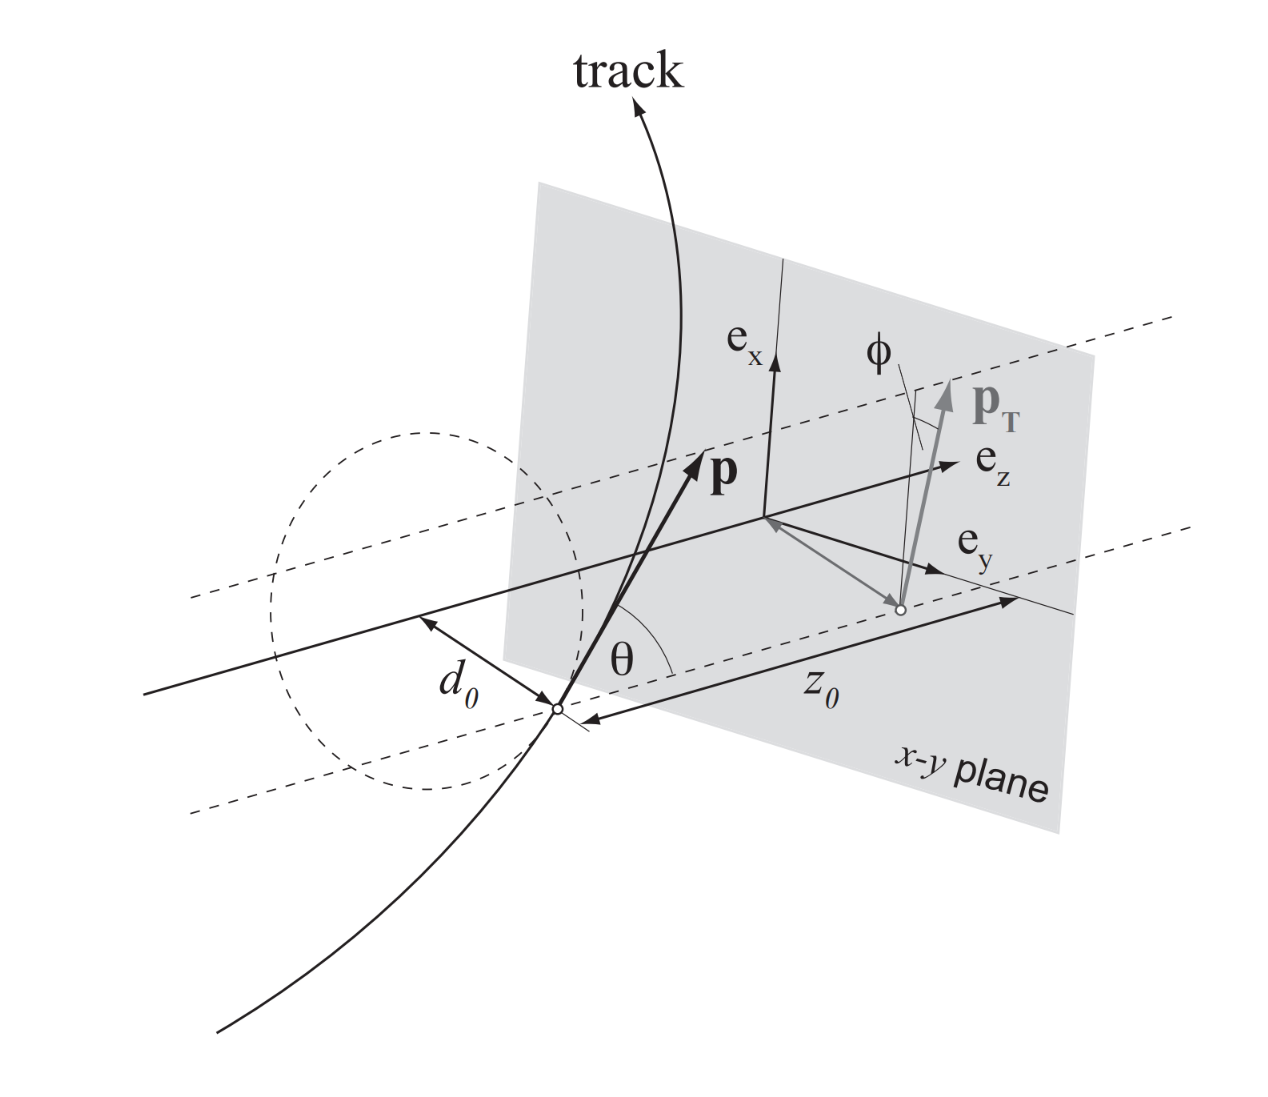
\includegraphics[width=\fullfig]{figures/perigee_rep.png}
\caption{An illustration of the perigee representation of track parameters for an example track. The charge is not directly shown, but is indicated by the direction of curvature of the track~\cite{atlas_extrapolation}.}
\label{fig:perigee_rep}
\end{figure}

This inside-out algorithm is complemented by an outside-in algorithm, which is used to find tracks from secondary particles, those produced in the decays or interactions of the primary particles inside the detector. 
As the name indicates, the outside-in algorithm begins by seeding tracks in the outermost layers of the inner detector, in the \ac{TRT}. 
The seed in this case is formed by a segment in the \ac{TRT}, and the track is propagated backwards into the \ac{SCT} before being refitted to use all the included points.
Some tracks are found with \ac{TRT} segments only, which can result from interactions with the detector following the \ac{SCT}.
Figure~\ref{fig:track_patterns} shows an example of the geometry of tracks formed by both algorithms, where the hits belonging to tracks found using the inside-out algorithm are highlighted in red, and the hits belonging to the tracks found using the outside-in algorithm are circled in black.
The figure highlights the presence of a large number of both primary and secondary tracks in a single event, as well as the overall large number of hits present in the inner detector.

\begin{figure}
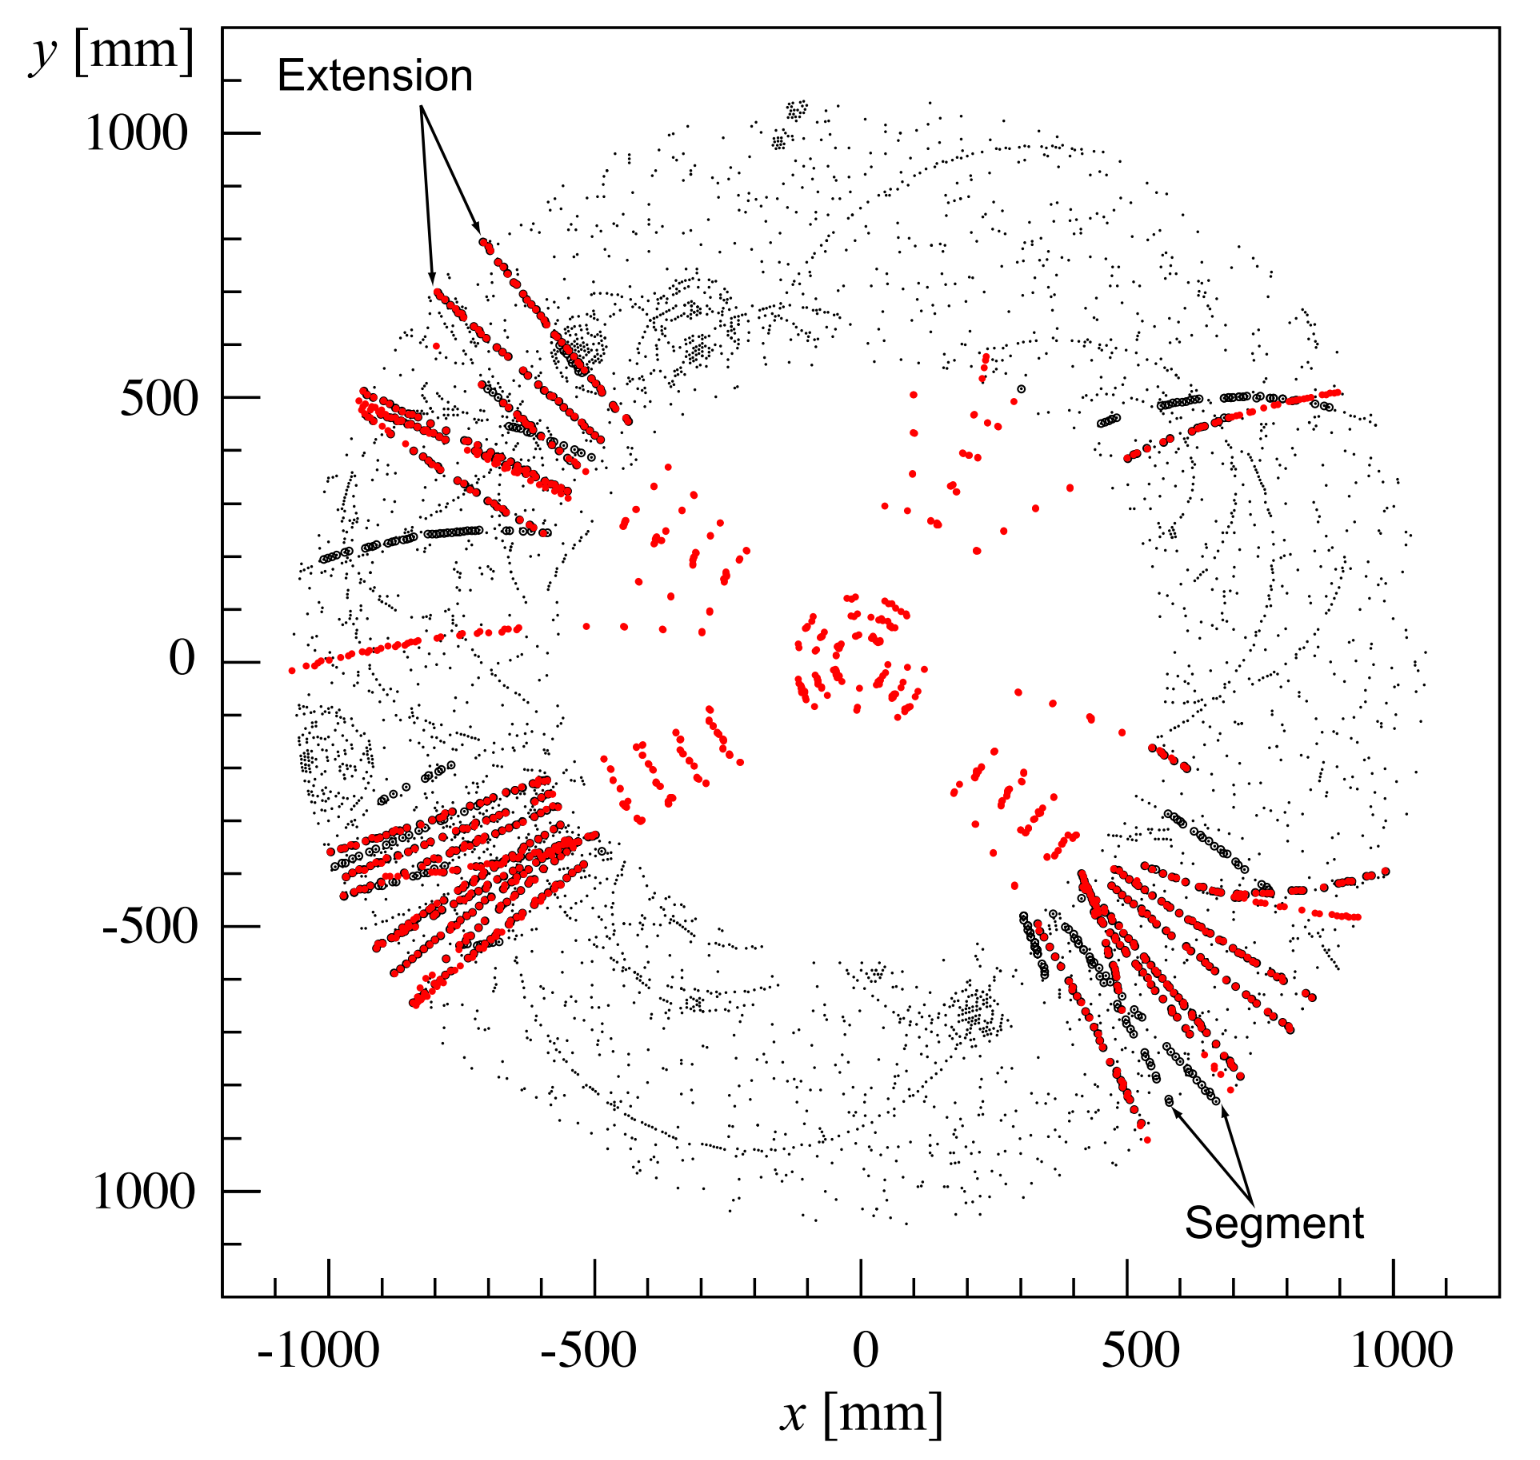
\includegraphics[width=\fullfig]{figures/track_patterns.png}
\caption{The $x$ and $y$ locations of the hits generated in a simulated $t\bar{t}$ event in the inner detector. The hits which belong to tracks formed using the inside-out algorithm are highlighted in red, while the hits which belong to tracks formed using the outside-in algorithm are circled in black. This figure does not include hits in the \ac{IBL}.}
\label{fig:track_patterns}
\end{figure}

The tracks resulting from these algorithms can be contaminated by nearby particles confusing the tracking algorithm in a high luminosity environment.
For example, enough hits present in the inner detector can lead to fake tracks from combinations of hits from multiple individual tracks.
Therefore, after the tracks are formed and fitted, additional quality requirements are imposed in order to reduce such backgrounds.
Most tracking applications require at least seven silicon hits, that is, seven hits between the Pixel detector and \ac{SCT}.
Then the tracks are required to have at most two holes in the Pixel detector, where holes are non-existing but expected measurements in a layer of the subdetector.
If the missing hit corresponds to an inactive module, however, it is not counted as a hole but instead as a hit for tracking as the lack of a measurement is expected in that case.
With these requirements, the inner detector achieves the reconstruction efficiencies shown in Figure~\ref{fig:track_reco_eff} as a function of \pt and $\eta$.
The efficiency ranges between 80\% and 90\% for the tight primary selection described above, and is maximized at high \pt and low $|\eta|$.

\begin{figure}
\subfloat[]{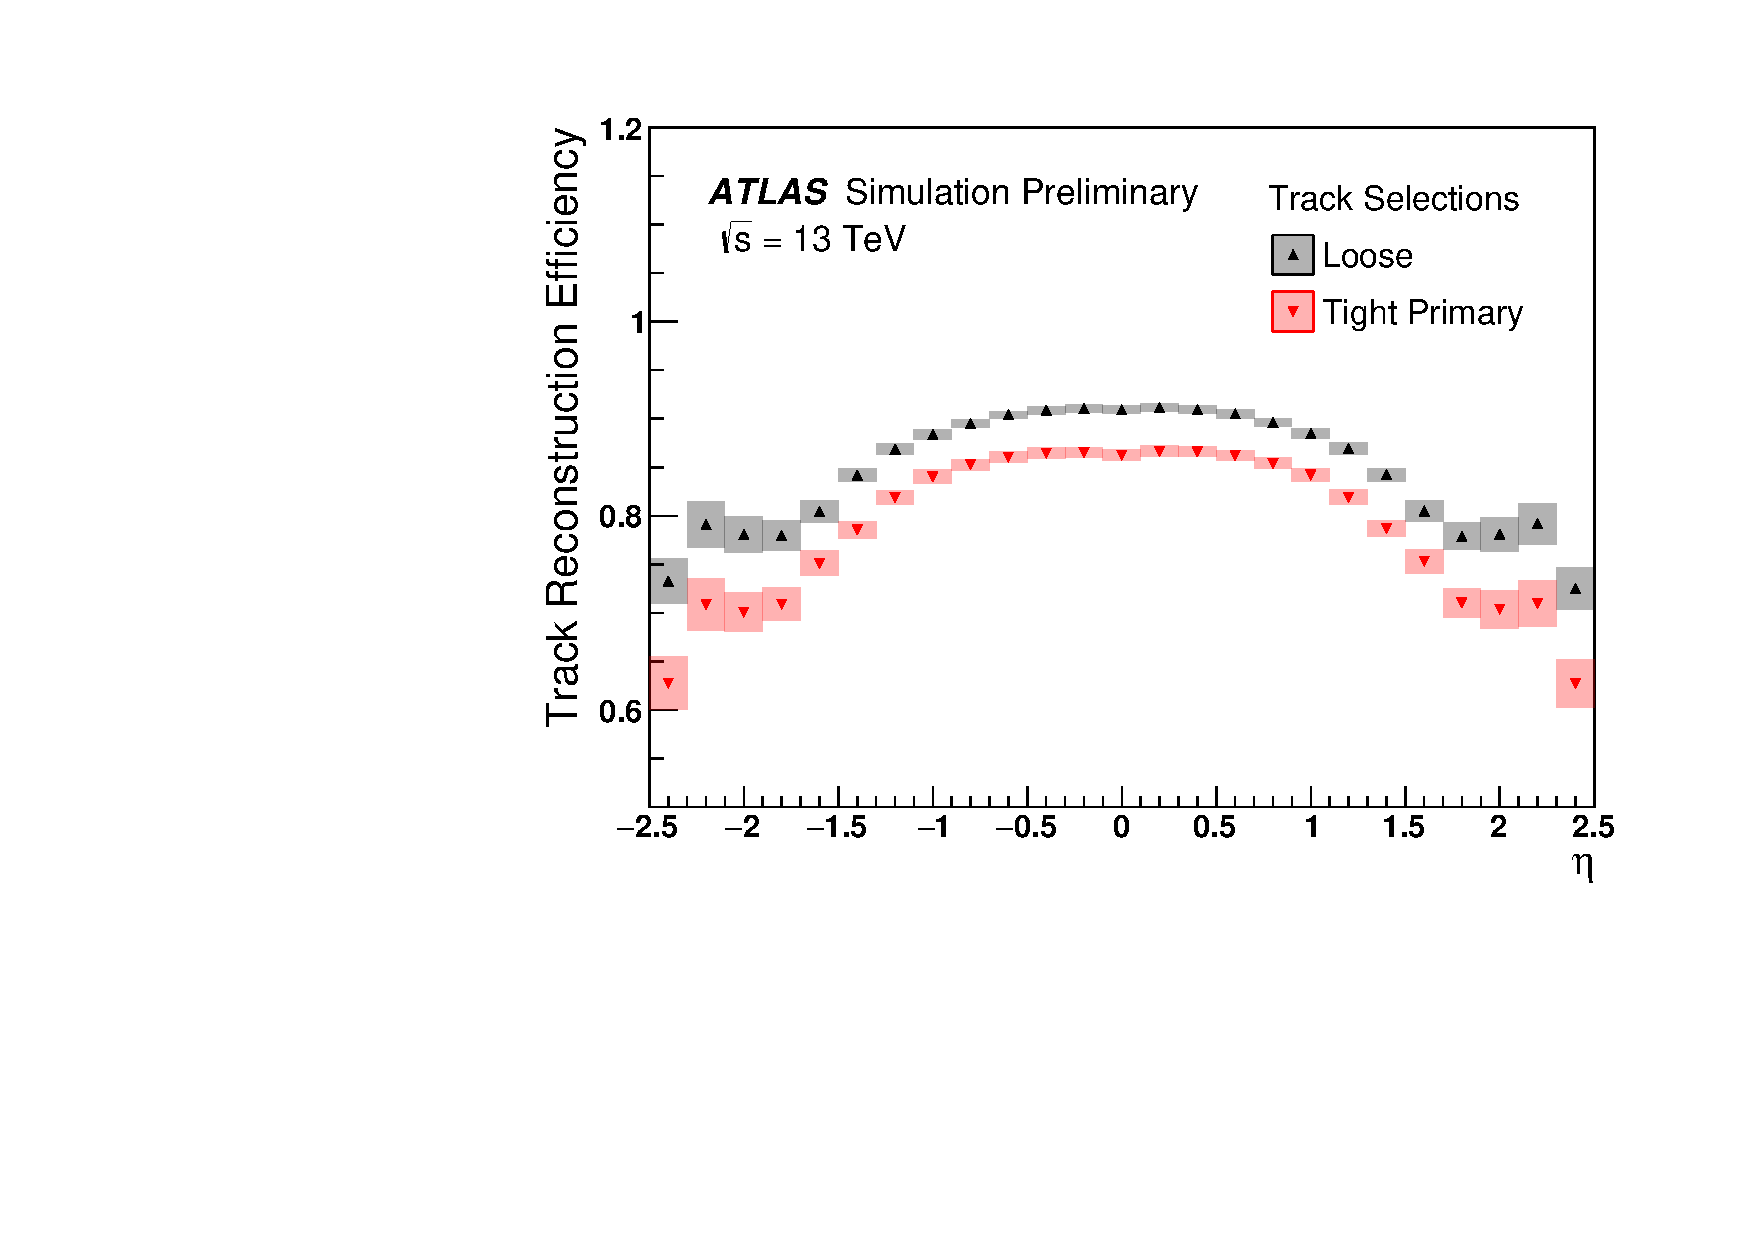
\includegraphics[width=\halffig]{figures/track_reco_eff_eta.pdf}}
\subfloat[]{\includegraphics[width=\halffig]{figures/track_reco_eff_pt.pdf}}
\caption{The tracking reconstruction efficiency as a function of (a) $\eta$ and (b) \pt~\cite{ATL-PHYS-PUB-2015-051}.}
\label{fig:track_reco_eff}
\end{figure}

\subsection{Pixel Neural Network}
\label{sec:pixelnn}

The hits in the Pixel detector are not typically confined to a single pixel, but rather the charge is spread over several pixels per layer which are grouped together into clusters.
The clustering of these pixels for isolated tracks is relatively straightforward; a connected component analysis identifies groups of neighboring pixels above the readout threshold~\cite{pixel_nn}.
Complications can arise in the high occupancy environment where hits from multiple particles can overlap in a single cluster.
Figure~\ref{fig:pixel_cluster_types} shows examples of clusters generated by a single isolated particle, two nearly overlapping particles, and a particle which emits a $\delta$-ray. 
A $\delta$-ray is a secondary electron which is generated with enough energy to escape a significant distance away from the original particle and to generate additional ionization.

\begin{figure}
\includegraphics[width=\fullfig]{figures/pixel_cluster_types.pdf}
\caption{Examples of the clusters formed in a single layer of the pixel detector for (a) a single isolated particle, (b) two nearly-overlapping particles, and (c) a particle which emits a $\delta$-ray~\cite{pixel_nn}.}
\label{fig:pixel_cluster_types}
\end{figure}

A series of neural-networks analyzes the shape of the clusters to determine how many particles produced the cluster and to estimate the positions of each of the particles within the cluster.
These allow for an identification of clusters caused by more than one particle or by a particle that emits a $\delta$-ray.
In a high-density tracking environment, the multiple position outputs can be used as the locations of individual hits to allow reconstruction of tracks which almost overlap and with a much better separation than is possible without the splitting of individual clusters.

\subsection{Pixel dE/dx}
\label{sec:pixel_dedx}

A hit in the Pixel detector corresponds to the voltage generated from ionization current rising above a threshold value that is tuned to consistently record the passing of \acp{MIP}. 
A larger amount of charge deposited results in a larger voltage, and a larger signal remains above the threshold for a longer period of time.
The \ac{ToT} is read out of the Pixel detector, and can be used to provide a measurement of the charge deposited in each pixel.
The charge measurements from each of the pixels included in a pixel cluster are summed to form one charge measurement per layer of the pixel detector.
That charge measurement, combined with the angle of incidence of the track and the known sizes of each detector element, can be converted into a measurement of \dedx, the ionization energy deposited per unit distance, measured in \MeVgcm. 
The \ac{IBL} only has sixteen available values (4 bits) of \ac{ToT} to readout, compared to the 256 available values (8 bits) in the remaining pixel layers.
To help alleviate this lack of range, the \ac{IBL} also records if it is in overflow: when the ionization is sufficient to generate a \ac{ToT} above the largest value that can be recorded in the 4 bits.
In the remaining layers, the charge value is lost if the hit is in overflow; however the significantly larger range of values makes this very rare in those layers.

The measurements across multiple layers are combined to form an average value of \dedx for the track as a whole.
Depending on where a charged particle is produced, it will traverse four Pixel layers and create four clusters on average.
It can produce as few as two clusters in the Pixel detector if it passes through inactive modules, and as many as five if is in a region of the detector where multiple modules overlap.
To reduce the influence of the typical long Landau tails of the distribution of \dedx deposits~\cite{pdg}, the average is calculated as a truncated mean of these clusters.
The value measured in the \ac{IBL} is removed if it is in overflow, as the measured value is not reliable in that case.
If a track has five measurements in the pixel detector, the two highest cluster values are removed.
If a track has two, three, or four measurements in the pixel detector, only the single highest cluster value is removed.
The remaining values are averaged to form the pixel \dedx.

\subsection{Vertex Reconstruction}
\label{sec:vertices}

A vertex represents the intersection of multiple tracks and corresponds to the location of an interaction.
If at least two charged particles result from the interaction, the intersection of their resulting tracks reveals its position with high precision.
Vertices are divided into two groups, primary vertices which correspond to the actual proton-proton collisions, and secondary vertices which correspond to decays of short-lived particles or interactions with the detector. 
Primary vertices are particularly important, as they can provide a precise location for the interaction which generated the observed particles.
Understanding that location is crucial in understanding the geometry of the event.

Primary vertices are reconstructed by iteratively identifying seeds from reconstructed tracks~\cite{ATLAS-CONF-2010-069}.
Each track's extrapolated $z$ position at the beamline forms a seed, and nearby tracks are fitted using that position as a point along their trajectory.
The goodness of fit with that vertex is considered for each track, measured in $\chi^2$. 
The final position of the vertex is determined by a fit to all of the considered tracks, where the contribution from each track is weighted according to the $\chi^2$ compatibility with that vertex and by the error on its position.
Any tracks that are displaced by more than 7$\sigma$ from that vertex are removed from the fit and used to seed a new vertex.
This procedure is iterated until no additional vertices can be found.

This procedure is typically performed twice.
The first set of vertices is used to fit a profile for the beamspot, which indicates the position of the intersection of beams in that particular bunch crossing.
The fitted beamspot then provides a constraint for the second attempt to locate primary vertices, where both the track fitting and seeding of vertices are required to be consistent with interactions occurring within the beamspot.
The vertex reconstruction algorithm achieves the efficiency shown in Figure~\ref{fig:vertex_reco_eff}, increasing from 83\% for vertices with two associated tracks and up to nearly 100\% for vertices with four or more associated tracks.

\begin{figure}
\includegraphics[width=\halffig]{figures/vertex_reco_eff.pdf}
\caption{The vertex reconstruction efficiency as a function of the number of associated tracks~\cite{ATL-PHYS-PUB-2015-026}.}
\label{fig:vertex_reco_eff}
\end{figure}


% ----------------------------------------

\section{Electrons and Photons}
\label{sec:egamma}

Electrons are measured as both a charged particle track and energy deposits in the electromagnetic calorimeter.
Photons, on the other hand, leave energy deposits in the electromagnetic calorimeter but do not produce a corresponding track.
Because the electromagnetic interactions with the calorimeter of both photons and electrons produces more photons and electrons, the behavior in the calorimeter is very similar and their is significant overlap in the reconstruction techniques for each.

The reconstruction of a photon or an electron in the calorimeter is based on clustering algorithms which identify groups of energy deposits~\cite{PERF-2013-03, ATLAS-CONF-2014-032, ATLAS-CONF-2012-123}.
For this purpose, the entire electromagnetic calorimeter is subdivided into a grid of 200 by 256 towers in the $\eta$ and $\phi$ directions, respectively, where the individual grid units have a size of $\Delta\eta = 0.025$ and $\Delta\phi = 0.025$.
These towers correspond to individual cells in the middle, coarsest layer of the \ac{EM} calorimeter, and in the remaining layers the cells are grouped together cover the same area in $\eta-\phi$ space.
The clustering begins by finding seeds with a sliding-window algorithm based on the towers: a window of 3 by 5 towers is formed and translated until the sum of the energy within the window is maximized.
If that energy is above 2.5 \GeV, then that region becomes a seed.
The choice of 2.5 \GeV was chosen to compromise between maximizing reconstruction efficiency while minimizing fake electron seeds from electronic noise or soft hadrons from additional interactions.
The seeds are rejected if the energy measured in the hadronic calorimeter behind the seed is large, as this typically indicates a hadron rather than an electron or photon.

Next, the inner detector tracks within a cone of $\Delta R = 0.3$ are compared to the location and energy of the seed.
Tracks are matched to the cluster if the extrapolation of the track to the energy-weighted center in the middle layer of the \ac{EM} calorimeter falls within $\Delta\phi < 0.2$ in the direction of the curvature of the track or $\Delta\phi < 0.05$ in the direction opposite of the curvature of the track.
If the seed matches with a track that originated from a primary vertex, the combination of track and electromagnetic cluster is reconstructed as an electron.
If the seed matches with a track that did not originate from a primary vertex, then the electromagnetic cluster is reconstructed as a converted photon.
And if there is no corresponding track in the inner detector, than the cluster is reconstructed as a photon.

After classification, the final clustering of the energy in the \ac{EM} calorimeter calorimeter is performed.
The classification must be done first, as the expected size of the energy deposits in the calorimeter are different for electrons and photons.
In the barrel region, the final clusters for electrons are formed in rectangles of 3 towers in the $\eta$-direction and 7 towers in the $\phi$-direction.
This asymmetric window accounts for the curving of the charged particles only in the $\phi$ direction.
For photons, the size of the rectangle is 3 towers by 5 towers.
In the endcap region, all object types are clustered in rectangles of 5 towers by 5 towers, as the effect of the magnetic field curvature is less pronounced in this region.
The sum of the energies in these clusters provide the final energy measurement for the electron or photon.

\subsection{Photon Identification}

The original requirement for constructing a photon cluster, a significant energy deposit in the electromagnetic calorimeter without a corresponding track or energy deposits in the hadronic calorimeter, is already effective in identifying photons.
However, there is a significant background for prompt photon production from the decays of pions, $\piz \rightarrow \gamma\gamma$.
These can be identified using the shape of the cluster in the narrow $\eta$ granularity in the first layer of the \ac{EM} calorimeter.

\subsection{Electron Identification}

Prompt electrons have a number of backgrounds, such as secondary electrons from hadron decays or misidentified hadronic jets, that can be rejected using additional information from the \ac{EM} calorimeter and the inner detector.
The most basic level of electron identification, referred to as Loose, makes requirements on the shower shapes in the high granularity first layer of the \ac{EM} calorimeter as well as the quality of the inner detector track.
It also requires a good match between the track and the calorimeter energy deposits and a small fraction of energy in the hadronic calorimeter behind the electromagnetic cluster.
ATLAS defines several additional working points, including MediumLL and TightLL, which provide progressively lower background rates for electrons by imposing additionally strict requirements on the above variables as well as new requirements like the impact parameter of the inner detector track or the comparison of the cluster energy to the momentum in the inner detector.
The LL designates that the requirement is based on a threshold on the output of a likelihood function using the above quantities as an input~\cite{ATLAS-CONF-2014-032}.

% ----------------------------------------

\section{Muons}
\label{sec:muons}

Muons produced in ATLAS first traverse the inner detector and leave behind a track as described in Section~\ref{sec:tracks}.
The muon then passes through the calorimeter, leaving behind a small, characteristic amount of energy, and then passes through the muon spectrometer where it produces hits in the \acp{MDT} or \acp{CSC}.
Muon tracks are formed from local segments of hits in each layer of the \acp{MDT} or \acp{CSC}, and then the final muon spectrometer track is formed by combining the two local segments~\cite{PERF-2015-10}.
When a track is reconstructed in both the inner detector and the muon spectrometer, the track is refitted to include the hits in both the inner detector and the muon spectrometer, and forms a combined muon.

In a few regions of the detector, a muon may fail to leave behind both a complete inner detector and muon system track.
For a very small fraction of the acceptance of the muon system, there is only one layer of muon chambers and a global muon system track is not formed.
In this case, as long as the track in the inner detector exists and geometrically matches to a segment, a segment-tagged muon is formed using momentum measurements from the inner detector.
In the region where the muon system has coverage but the inner detector does not, $2.5 < |\eta| < 2.7$, a stand-alone muon is formed which uses only information from the muon system.
And for muons produced within one of the few holes in the muon system, including $|\eta| < 0.1$, the characteristic energy deposits in the calorimeter can be used to tag an inner detector track as a calo-tag muon.
These additional categories are used to achieve high efficiency over a larger range of acceptance, but the combined muons are the most reliable.

\subsection{Muon Identification}
\label{sec:muon_id}

The various types of muons are incorporated into three working points: Loose, Medium, and Tight, which reflect the increasing muon purity for each of the selections definitions.
Tight muons include only combined muons with a good track fit quality and momentum resolution and at least two hits in a precision muon system layer.
Medium muons include those in tight as well as combined muons with one precision hit and one precision hole, where hole is defined in the same way as in Section~\ref{sec:tracks}.
The medium working point also includes stand-alone muons with $|\eta| > 2.5$ and at least two hits in precision layers.
And finally the loose working point includes both medium and tight muons, but additional includes segment-tagged and calo-tagged muons in the region $|\eta| < 0.1$.
The reconstruction efficiencies for muons with $\pt > 20\ \GeV$ range from 91.8\% for tight muons and up to 98.1\% for loose muons~\cite{PERF-2015-10}.

% ----------------------------------------

\section{Jets}
\label{sec:jets}

A jet does not directly correspond to a physical particle, unlike all of the reconstructed objects described above, but instead tries to capture the conical cascade of particles produced in the hadronization of a quark or gluon from the proton-proton collision.
The hadronization process creates a very large number of collimated particles, with a high enough density that individually reconstructing all of the produced particles in the calorimeter is not possible within ATLAS.
However most analyses are interested only in the kinematics of the particle which produced the cascade, rather than the individual products.
Therefore, jets are a useful tool to measure the combined energy and direction of the ensemble of products and thus represents the kinematics of the original.
Jet algorithms are very generic and can be used to group together a number of types of objects to form aggregate representations.
For example, truth particles in simulation can be grouped in truth jets, or tracks from the inner detector can be grouped together to form track jets. 
This section, however, will focus on calorimeter jets which take topoclusters of energy deposits in the calorimeter as inputs and produce a combined object which represents the energy measured by the calorimeter and the location where it was deposited.

\subsection{Topological Clustering}

Hadrons often deposit their energy into multiple individual cells in both the electromagnetic and hadronic calorimeters.
The purpose of topological clustering is to group cells in all three dimensions into clusters that represent a single energy deposit.
The procedure must be robust enough to reject noise fluctuations in the cell energy measurements that can come from both electronic noise and additional low energy particles produced in pileup activity.
The background level of calorimeter noise is called \signoise, and is an important component of the topological clustering.

The topological clusters are formed in a three step process called the 4-2-0 threshold scheme, which uses three energy thresholds to build up a cluster from cells~\cite{PERF-2014-07}.
First, any cells with a measured energy above 4\signoise are identified as seed cells. 
The cells adjacent to the seed cells with a measured energy above 2\signoise are called secondary cells.
All of the cells which are adjacent to a secondary cell with $E_\mathrm{cell} > 2\signoise$ are also labeled secondary cells.
Tertiary cells are those immediately adjacent to a seed or secondary cell with a measured energy above zero.
Adjacency in this sense is defined in three dimensions, cells are adjacent if they are neighbors within a layer but also if they have the same $\eta-\phi$ coordinates but are in adjacent layers or even in an adjacent layer in another calorimeter.

From these definitions, clusters are built by resolving the seeds in order of significance, the ratio $E_{\mathrm{cell}}/\signoise$.
All adjacent secondary cells to the highest significance seed are added to that seed's topocluster, and any of those cells which would also have qualified as seeds are removed from the list of seeds.
Once all of the secondary cells have been added, the tertiary cells are then added to that cluster as well.
This procedure is then iterated until no seeds remain, forming the first round of topoclusters.

It is also useful to split topoclusters into multiples if local maxima are present within the topocluster, as clusters produced by multiple nearby particles can merge.
The splitting process begins by finding local maxima cells in the middle layer of the calorimeters with a minimum energy of 500 \MeV and at least four neighboring secondary cells.
These requirements reduce the likelihood to split a cluster due to random fluctuations, as the middle layers provide the most reliable energy measurements.
Cells between two local maxima can then be shared between two clusters to account for overlapping contributions from two particles. The energy sharing is weighted by the energy of each cluster as well as the distance of the cell to the centroid of that cluster.

The energies of all the cells in the cluster are then summed together to form the energy of that cluster.
The energy needs to be corrected for the various losses expected in the calorimeter, as described in Section~\ref{sec:calorimetry}.
The simplest correction, scaling the measured energy by the sampling fraction, brings the cluster energies to the \ac{EM} scale.
It is called the \ac{EM} scale because it accurately describes the energy of electromagnetic showers.

Another scale is defined to improve accuracy for hadronic processes, the \ac{LCW} scale, that helps to correct for the expected variations in hadronic energy deposits.
The \ac{LCW} correction first determines if the shower is hadronic or electromagnetic, based on the depth of the shower and the cluster energy density.
For hadronic showers, the energy is corrected for calorimeter non-compensation, an effect which reduces the measured energy of hadronic showers because some of the energy goes into invisible processes like the break up of nuclei.
All clusters are then corrected for energy that may be deposited in uninstrumented regions in that cluster's location in the calorimeter, and they are also corrected with an estimate of how much energy falls outside the extent of the cluster based on its shape and the deposit type.

\subsection{Jet Algorithms}
Using the topological clusters as inputs, a jet algorithm groups them together into a collection of adjacent energy deposits that is intended to correspond to a single process~\cite{ATL-PHYS-PUB-2015-036}.
Jet algorithms need a few key characteristics to be usable for physics analysis.
First, the jets produced by the algorithm should have little dependence on the addition of soft particles to the event (infrared safety), as a negligible addition of energy should not significantly modify the event topology.
The jets produced by the algorithm should also be collinear safe: a single quark replaced by two, parallel quarks with half the original's momentum should not change the resulting jets.
This requirement is important as the jets are intended to capture only the properties of the aggregate and not those of individual particles.
And finally the algorithm needs to be sufficiently simple and fast to be used for the large rate of collected proton-proton collisions on ATLAS.

The most commonly used algorithm on ATLAS that satisfies these requirements is called the anti-$k_t$ algorithm~\cite{antikt}.
The anti-$k_t$, in brief, relies on iteratively combining the input objects that are closest together, where closest is defined by a particular distance metric, $d_{i,j}$, where the index $i$ represents the combination constructed so far and $j$ is an additional object being considered.
The combinations stop when the closest remaining object is the beam itself, where the distance to the beam is called $d_{i,B}$. 
An entire class of algorithms follows this procedure with the following distance metrics

\begin{align}\label{eq:antikt}
d_{i,j} &= \min(k_{ti}^{2p}, k_{tj}^{2p}) \frac{\Delta_{ij}^2}{R^2} \\
d_{i,B} &= k_{ti}^{2p}
\end{align}

where $\Delta_{i,j} = (y_i - y_j)^2 + (\phi_i - \phi_j)^2$, $k_{ti}$ is the transverse momentum of the object, $y$ is the rapidity, and $p$ is a parameter of the algorithm.
Anti-$k_t$ is the particular case where $p = -1$, and is a choice that results in an algorithm that is both infrared and collinear safe.

The algorithm is repeated until there are no input objects remaining, which results in a series of jets. 
Each jet has a complete four momentum from the combination of its input clusters, where the combinations assume a mass of zero.
The jet energies then need to be calibrated to attempt to match the energy of the object which produced the jet.

\subsection{Jet Energy Scale}
\label{sec:reco_jes}

Though the \ac{LCW} scheme attempts to correct the topoclusters to reflect the true deposited energy, the correction does not fully account for energy lost within the calorimeters.
Because of these effects, the original reconstructed jet energy does not reflect the true energy of the particle which initiated the jet.
Therefore it is necessary to additionally correct the reconstructed jet itself, in addition to the corrections on the inputs.
This correction is referred to as the \ac{JES}, which combines several individual steps of calibration~\cite{ATLAS-CONF-2015-002}.

The first calibration step corrections the direction of the jet to ensure that it points back to the primary vertex.
Next, the energy of the jet is corrected for pileup by subtracting the expected contribution from pileup based on the momentum, $\eta$, and area of the jet as well as the number of reconstructed vertices and the expected number of interactions per crossing, $\mu$.
The largest single correction adjusts the jet energy and pseudorapidity to attempt to match the energy and pseudorapidity of the parton which produced it.
This correction is measured in simulation by comparing the reconstructed jet energies to the energy of the truth particle which produced it.
However the simulation is not relied on alone to estimate this correction, and an additional step applies an additional energy correction based on in-situ measurements in data.
These corrections come from various techniques which measure jet energies indirectly by balancing them with other, well-measured objects.
In the central region ($|\eta| < 1.2$), jets are balanced against photons and the leptonic decays of Z bosons and high momentum jets ($p_T > 210$ GeV) are also balanced against multiple smaller jets in multijet events.
Jets at larger pseudorapidities, above $|\eta| = 1.2$, are calibrated by balancing with lower pseudorapidity jets.

These steps introduce a number of systematic uncertainties, referred to as the \ac{JES} uncertainty.
The largest of these comes from the in-situ measurements, which are statistically limited in measuring high momentum and high pseudorapidity jets.
The total, fractional \ac{JES} uncertainty is shown as a function of $p_T$ in Figure~\ref{fig:reco_jesunc}.
The uncertainty falls to a minimum value of just over 1.0\% around a few hundred \GeV, and rises again at high momentum because of the difficulty of measuring jet balance in data above 2-3 \TeV.
The uncertainty is also minimized at low $|\eta|$, and grows at large $|\eta|$ again where making in-situ measurements is difficult.
This technique does not actually provide a measurement of the uncertainty for the highest energy jets, above 3 \TeV, because there are not enough measured data events to provide them.
An alternative method for deriving the \ac{JES} and \ac{JES} uncertainty that can be used even for very high $p_T$ jets will be discussed in Chapter~\ref{ch:jes}.

\begin{figure}
\includegraphics[width=\fullfig]{figures/reco_jes_pt.png}
\caption{The total, fractional \ac{JES} uncertainties estimated for 2015 data as a function of jet $p_T$.}
\label{fig:reco_jesunc}
\end{figure}

% ----------------------------------------

\section{Missing Transverse Energy}
\label{sec:missing_energy}

Among stable \ac{SM} particles, only the neutrino cannot be directly measured in the ATLAS detector. 
Because the neutrino carries neither electric nor color charge, it is very unlikely to interact with the tracking detectors or the calorimeters, and instead passes through the detector completely unobserved.
Some particles which have been conjectured to exist, like the \ac{LSP} in many \ac{SUSY} models, would also have the same behavior.
Therefore, it is important for ATLAS to provide some way to assess the momentum carried away by a neutral, colorless particle.
This can be accomplished through a measurement of missing energy in the transverse direction, or \met, which quantifies the momentum imbalance of the observed particles.
From the conservation of momentum and the lack of the initial momentum in the transverse plane in the proton-proton collisions, any imbalance of momentum can be inferred to be carried away by an unmeasured particle.

\met is more precisely defined as the magnitude of the vector sum of the $(p_x,p_y)$ components of each observed object's momentum.
The definition is simple, but there can be significant complexity in defining the inputs.
As of Run 2, ATLAS uses a common algorithmic approach to carefully calculate missing energy, but each analysis is free to define it's own inputs.
For the analysis discussed throughout this thesis, the missing energy inputs consist of the electrons, photons, muons, and jets discussed in the previous sections, in addition to a track-based term that accounts for the contribution of low \pt particles (soft term).

To produce the most precise measurement of \met, it is important to use the best representation of the momentum of each of the input objects, which can often be reconstructed as multiple different types in a single event.
For example, an electron can be reconstructed separately as an electron (Section~\ref{sec:egamma}) and a jet (Section~\ref{sec:jets}), but the electron representation has the highest precision for reconstructing the true electron momentum.
To ensure no duplications in the \met definition, the inputs are collectively considered for overlap removal.
Only the most precise object type is kept for objects that fall within a cone of $\Delta R < 0.2$ for pairs of electrons and jets and a cone of $\Delta R < 0.4$ for other pair types.

The fully reconstructed objects do not include all of the energy within the events, as some clusters do not enter into a jet and some tracks are not classified as electrons or muons.
These momentum carried by these objects is accounted for in a soft-term, which tallies all of the energy carried by the particles too soft to form separate objects.
The track soft term uses only tracking information to estimate the contribution of soft objects, and does so by vectorially summing the momentum of all well-reconstructed tracks with momentum above 400 \MeV that are not associated to other objects.

All of these contributions together give a single \met value for a given event.
The direction of that missing energy is taken as opposite the vector sum of all the constituents, to correspond to the momentum an invisible particle would have to have to make the event balanced.
Depending on the context, this missing energy can be considered the energy of a neutrino or an \ac{LSP}, with a large missing energy being a common signal criteria for searches for new physics.

% ----------------------------------------


%\ctparttext{You can put some informational part preamble text here.}
\part{Calorimeter Response}
\label{part:calorimeter}
\chapter{Response Measurement with Single Hadrons}

\newcommand*{\pL}{\ensuremath{\Lambda}\xspace}
\newcommand*{\pLB}{\ensuremath{\bar{\Lambda}}\xspace}
\newcommand*{\pKS}{\ensuremath{K_\text{S}^{0}}\xspace}
\newcommand*{\pKL}{\ensuremath{K_L}\xspace}
\newcommand*{\pP}{\ensuremath{p}\xspace}
\newcommand*{\pAP}{\ensuremath{\bar{p}}\xspace}
\newcommand*{\pip}{\ensuremath{\pi^+}\xspace}
\newcommand*{\pim}{\ensuremath{\pi^-}\xspace}
\newcommand*{\piz}{\ensuremath{\pi^0}\xspace}
\newcommand*{\ep}{\ensuremath{E/p}\xspace}
\newcommand*{\epav}{\ensuremath{\langle E/p \rangle}\xspace}
\newcommand*{\epcor}{\ensuremath{\langle E/p \rangle_{\mathrm{COR}}}\xspace}
\newcommand*{\epbg}{\ensuremath{\langle E/p \rangle_{\mathrm{BG}}}\xspace}
\newcommand*{\Ea}{\ensuremath{E_a}\xspace}
\newcommand*{\QGSP}{\texttt{QGSP\_BERT}\xspace}
\newcommand*{\FTFP}{\texttt{FTFP\_BERT}\xspace}


\label{ch:singlehadrons}
% --------------------------------------------------------------------------------

As discussed in Section~\ref{sec:jets}, colored particles produced in collisions hadronize into jets of multiple hadrons.
One approach to understanding jet physics in the ATLAS calorimetry is to evaluate the calorimeter response to those individual hadrons; measurements of individual hadrons can be used to build up an understanding of the jets that they form.
The redundancy of the momentum provided by the tracking system and the energy provided by the calorimeter provides an opportunity to study calorimeter response using real collisions, as described further in Section~\ref{sec:inclusive}.

Calorimeter response includes a number of physical effects that can be extracted to provide insight into many aspects of jet modeling.
First, many charged hadrons interact with the material of the detector prior to reaching the calorimeters and thus do not deposit any energy.
Comparing this effect in data and simulation is a powerful tool in validating the interactions of particles with the material of the detector and the model of the detector geometry in simulation, see Section~\ref{sec:zero_fraction}.
The particles which do reach the calorimeter deposit their energy into individual cells, which are then clustered to measure full energy deposits.
Comparing the response in data to simulated hadrons provides a direct evaluation of noise in the calorimeters, the showering of hadronic particles, and the energy deposited by particles in matter (Section~\ref{sec:response}). 
These measurements are extended to explore several additional effects, such as the dependence on charge, in Section~\ref{sec:additional}. 

The above studies all use an inclusive selection of charged particles, which are comprised predominantly of pions, kaons, and (anti)protons.
It is also possible to measure the particle types separately to evaluate the simulated interactions of each particle, particularly at low energies where differences between species are very relevant.
Pions and (anti)protons can be identified through decays of long-lived particles, in particular $\Lambda$, $\overline{\Lambda}$, and $K_{S}^{0}$, and then used to measure response as described above.
This is discussed in detail in Section~\ref{sec:identified}.

Together, these measurements in data provide a thorough understanding of the way hadrons interact with the ATLAS detector and can be used to build up a description of jets, as seen in Chapter~\ref{ch:jes}.
The results in this chapter use data collected at 7 and 8 \TeV collected in 2010 and 2012, respectively.
Both are included as the calorimeter was repaired and recalibrated between those two data-taking periods.
Both sets of data are compared to an updated simulation that includes new physics models provided by \texttt{Geant4}~\cite{GEANT4} and improvements in the detector description~\cite{PERF-2011-08,PERF-2013-05}.
These results are published in \ac{EPJC}~\cite{PERF-2015-05} and can be compared to a similar measurement performed in 2009 and 2010~\cite{PERF-2011-05}, which used the previous version of the simulation framework~\cite{SOFT-2010-01}.

% ----------------------------------------
\section{Dataset and Simulation}

\subsection{Data Samples}
The two datasets used in this chapter are taken from dedicated low-pileup runs where the fraction of events with multiple interactions was negligible, to facilitate measurement of isolated hadrons.
The 2012 dataset at $\sqrt{s} = 8$ \TeV contains 8 million events and corresponds to an integrated luminosity of 0.1 nb\tsup{-1}.
The 2010 dataset at $\sqrt{s} = 7$ \TeV contains 3 million events and corresponds to an integrated luminosity of 3.2 nb\tsup{-1}.
The latter dataset was also used in the 2010 results~\cite{PERF-2011-05}, but it has since been reanalyzed with an updated detector description for the material and alignment.

\subsection{Simulated Samples}
The two datasets above are compared to simulated single-, double-, and non-diffractive events generated with \texttt{Pythia8}~\cite{PYTHIA8} using the A2 configuration of hadronization~\cite{AU2} and the MSTW 2008 parton-distribution function set~\cite{MSTW,MSTW2}.
The conditions and energies for each run are matched in the two simulations.

To evaluate the interaction of hadrons with detector material, the simulation uses two different collections of hadronic physics models, called physics lists, in \texttt{Geant4 9.4}~\cite{G4hadronics}.
The first, \QGSP, combines the Bertini intra-nuclear cascade~\cite{BERT21,BERT22,BERT23} below 9.9 \GeV, a parametrized proton inelastic model from 9.5 to 25 \GeV~\cite{GHEISHA20}, and a quark-gluon string model above 12 \GeV~\cite{QGS15,QGS16,QGS17,QGS18,QGS19}. 
The second, \FTFP, combines the Bertini intra-nuclear cascade~\cite{BERT21,BERT22,BERT23} below 5 \GeV and the Fritiof model~\cite{FTF24,FTF25,FTF26,FTF27} above 4 \GeV.
In either list, \texttt{Geant4} enforces a smooth transition between models where multiple models overlap.

\subsection{Event Selection}
\label{sec:inclusive_selection}
The event selection for this study is minimal, as the only requirement is selecting good-quality events with an isolated track. 
Such events are triggered by requiring at least two hits in the minimum-bias trigger scintillators. 
After trigger, each event is required to have exactly one reconstructed vertex, and that vertex is required to have four or more associated tracks.

The particles which enter into the response measurements are first identified as tracks in the inner detector.
The tracks are required to have at least 500 \MeV of transverse momentum.
To ensure a reliable momentum measurement, these tracks are required to have at least one hit in the pixel detector, six hits in the SCT, and small longitudinal and transverse impact parameters with respect to the primary vertex~\cite{PERF-2011-05}.
For the majority of the measurements in this chapter, the track is additionally required to have 20 hits in the TRT, which significantly reduces the contribution from tracks which undergo nuclear interactions.
This requirement and its effect is discussed in more detail in Section~\ref{sec:additional}. 
In addition, tracks are rejected if there is another track which extrapolates to the calorimeter within a cone of $\Delta R = \sqrt{(\Delta\phi)^2 + (\Delta\eta)^2} < 0.4$.
This requirement guarantees that the contamination of energy from nearby charged particles is negligible~\cite{PERF-2011-05}.

% ----------------------------------------

\section{Inclusive Hadron Response}
\label{sec:inclusive}

The calorimeter response is more precisely defined as the ratio of the measured calorimeter energy to the true energy carried by the particle, although this true energy is unknown. 
For charged particles, however, the inner detector provides a very precise measurement of momentum (with uncertainty less than 1\%) that can be used as a proxy for true energy.
The ratio of the energy deposited by the charged particle in the calorimeter, $E$, to its momentum measured in the inner detector $p$, forms the calorimeter response measure called \ep.
Though the distribution of \ep contains a number of physical features, this study focuses on the trends in two aggregated quantities: \epav, the average of \ep within a given subset of particles, and the zero fraction, the fraction of particles with no associated energy in the calorimeter.

The calorimeter energy assigned to a track particle is defined using clusters. 
The clusters are formed using a 4--2--0 algorithm~\cite{TopoClusters} that begins with seeds requiring at least 4 times the average calorimeter noise. 
The neighboring cells with at least twice that noise threshold are then added to the cluster, and all bounding cells are then added with no requirement. 
This algorithm minimizes noise contributions through its seeding process, and including the additional layers improves the energy resolution~\cite{Speckmayer}.
The clusters are associated to a given track if they fall within a cone of $\Delta R = 0.2$ of the extrapolated position of the track, which includes about 90\% of the energy on average~\cite{PERF-2011-05}.
This construction is illustrated in Figure~\ref{fig:eoverp_cartoon}.

\begin{figure}[htbp]
\centering
\subfloat[]{
  \includegraphics[width=.4\textwidth]{figures/SignalDiagram.png}
}
\subfloat[]{
  \includegraphics[width=.4\textwidth]{figures/BGDiagram.png}
}
\caption{An illustration (a) of the \ep variable used throughout this paper. The red energy deposits come from the charged particle targeted for measurement, while the blue energy deposits are from nearby neutral particles and must be subtracted. The same diagram (b) for the neutral-background selection, described in Section~\ref{sec:neutral_bg}.}
\label{fig:eoverp_cartoon}
\end{figure}

\subsection{E/p Distribution}

The \ep distributions measured in both data and simulation are shown in Figure~\ref{fig:eoverp} for two example bins of track momentum and for tracks in the central region of the detector. 
These distributions show several important features of the \ep observable.
The large content in the bin at $E=0$ comes from tracks that have no associated cluster, which occurs due to interactions with detector material prior to reaching the calorimeter or the energy deposit being insufficiently large to generate a seed, and are discussed in Section~\ref{sec:zero_fraction}.
The small negative tail comes from similar tracks that do not deposit any energy in the calorimeter but are randomly associated to a noise cluster.
The long positive tail above 1.0 comes from the contribution of neutral particles.
Nearby neutral particles deposit (sometimes large) additional energy in the calorimeter but do not produce tracks in the inner detector, so they cannot be rejected by the track isolation requirement.
Additionally the peak and mean of the distribution falls below 1.0 because of the loss of energy not found within the cone as well as the non-compensation of the calorimeter.

The data and simulation share the same features, but the high and low tails are significantly different.
The simulated events tend to overestimate the contribution of neutral particles to the long tail, an effect which can be isolated and removed as discussed in Section~\ref{sec:neutral_bg}. 
Additionally, the simulated clusters have less noise on average, although this is a small effect on the overall response.

\begin{figure}[htbp]
\centering
\subfloat[]{
  \includegraphics[width=\halffig]{figures/dvmc12_eoverp_layer01_calib01_eta01_p03_q00_nc00_trt00.pdf}
}
\subfloat[]{
  \includegraphics[width=\halffig]{figures/dvmc12_eoverp_layer01_calib01_eta01_p05_q00_nc00_trt00.pdf}
}
\caption{The \ep distribution and ratio of simulation to data for isolated tracks with (a) $|\eta| < 0.6$ and $1.2 < p /\GeV < 1.8$ and (b) $|\eta| < 0.6$ and $2.2 < p /\GeV < 2.8$.}

\label{fig:eoverp}
\end{figure}

\subsection{Zero Fraction}
\label{sec:zero_fraction}

The fraction of particles with no associated clusters, or similarly those with $E \leq 0$, reflects the modeling of both the detector geometry and hadronic interactions.
The zero fraction is expected to rise as the amount of material a particle traverses increases, while it is expected to decrease as the particle energy increases.
This dependence can be seen in Figure~\ref{fig:zerofracincl}, where the zero fraction in data and simulation is shown as a function of momentum and the amount of material measured in interaction lengths.
The trends are similar between the 2010 and 2012 measurements.
The zero fraction decreases with energy as expected.
The amount of material in the detector increases with $\eta$, which provides a distribution of interaction lengths.
As the data and simulation have significant disagreement in the zero fraction over a number of interaction lengths, the difference must be primarily from the modeling of hadronic interactions with detector material and not just the detector geometry.

There is also a noticeable difference between positive and negative tracks at low momentum, which reflects the difference in response between protons and antiprotons.
Antiprotons have significant model differences in the two physics lists, \QGSP and \FTFP, and this is evident in the lowest momentum bin of the data to simulation ratio.
This difference is explored further in Section~\ref{sec:identified}.


\begin{figure}[htbp]
\centering
\subfloat[]{
  \includegraphics[width=\halffig]{figures/dvmc_ezero_layer01_calib01_eta01_q02_nc00_trt00.pdf}
}
~
\subfloat[]{
  \includegraphics[width=\halffig]{figures/dvmc_ezero_layer01_calib01_eta01_q01_nc00_trt00.pdf}
}
\\
\subfloat[]{
  \includegraphics[width=\halffig]{figures/ezero_intlen_q02.pdf}
}
~
\subfloat[]{
  \includegraphics[width=\halffig]{figures/ezero_intlen_q01.pdf}
}
\caption{The fraction of tracks as a function (a, b) of momentum, (c, d) of interaction lengths with $E \leq 0$ for tracks with positive (on the left) and negative (on the right) charge.}
\label{fig:zerofracincl}
\end{figure}


\subsection{Neutral Background Subtraction}
\label{sec:neutral_bg}

The isolation requirement on hadrons is only effective in remove energy contribution from nearby charged particles. 
Nearby neutral particles, predominantly photons from \piz decays, also add their energy to the calorimeter clusters, but mostly in the electromagnetic calorimeter. 
It is possible to measure this contribution, on average, using late-showering hadrons that minimally ionize in the electromagnetic calorimeter. 
Such particles are selected by requiring that they deposit less than 1.1 \GeV in the EM calorimeter within a cone of $\Delta R < 0.1$ around the track. 
To ensure that these particles are well measured, they are additionally required to deposit between 40\% and 90\% of their energy in the hadronic calorimeter within the same cone. 

These particles provide a clean sample to measure the nearby neutral background because they do not deposit energy in the area immediately surrounding them in the EM calorimeter, as shown in Figure~\ref{fig:eoverp_cartoon}.
So, the energy deposits in the region $0.1 < \Delta R < 0.2$ can be attributed to neutral particles alone.
To estimate the contribution to the whole cone considered for the response measurement, that energy is scaled by a geometric factor of 4/3. 
This quantity, \epbg, measured in aggregate over a number of particles, gives the contribution to \epav from neutral particles in the EM calorimeter. 
Similar techniques were used in the individual layers of the hadronic calorimeters to show that the background from neutrals is negligible in those layers~\cite{PERF-2011-05}. 

The distribution of this background estimate is shown in Figure~\ref{fig:eoverp_background}. 
Although the simulation captures the overall trend, it significantly overestimates the neutral contribution for tracks with momentum between 2 and 8 \GeV.
This effect was also seen in the tails of the \ep distributions in Figure~\ref{fig:eoverp}.
This difference is likely due to the modeling of coherent neutral particle radiation in \texttt{Pythia8}, as the discrepancy does not depend on $\eta$ and thus is unlikely to be a mismodeling of the detector.
This difference can be subtracted to form a corrected average \ep, as in Section~\ref{sec:response}.

\begin{figure}[htbp]
\centering
\subfloat[]{
  \includegraphics[width=\halffig]{figures/dvmc_epbg_layer01_calib01_eta01_q00_nc00_trt02.pdf}
}
~
\subfloat[]{
  \includegraphics[width=\halffig]{figures/dvmc_epbg_layer01_calib01_eta02_q00_nc00_trt02.pdf}
}
\\
\subfloat[]{
  \includegraphics[width=\halffig]{figures/dvmc_epbg_layer01_calib01_p03_q00_nc00_trt02.pdf}
}
~
\subfloat[]{
  \includegraphics[width=\halffig]{figures/dvmc_epbg_layer01_calib01_p04_q00_nc00_trt02.pdf}
}
\caption{\epbg as a function of the track momentum for tracks with (a) $|\eta| < 0.6$, (b) $0.6 < |\eta| < 1.1$, and as a function of the track pseudorapidity for tracks with (c) $1.2 < p / \GeV < 1.8$, (d) $1.8 < p / \GeV < 2.2$.}
\label{fig:eoverp_background}
\end{figure}

\subsection{Corrected Response}
\label{sec:response}

Figure~\ref{fig:eoverp_corrected} shows \epcor as a function of momentum for several bins of pseudorapidity. 
This corrected $\epcor \equiv \epav - \epbg$ measures the average calorimeter response without the contamination of neutral particles. 
It is the most direct measurement of calorimeter response in that it is the energy measured for fully isolated hadrons. 
The correction is performed separately in data and simulation, so that the mismodeling of the neutral background in simulation is removed from the comparison of response. 
The simulation overestimates the response at low momentum by about 5\%, an effect that can be mostly attributed to the underestimation of the zero fraction mentioned previously.

\begin{figure}[htbp]
\centering
\subfloat[]{
  \includegraphics[width=\halffig]{figures/dvmc_epcor_layer01_calib01_eta01_q00_nc00_trt02.pdf}
}
~
\subfloat[]{
  \includegraphics[width=\halffig]{figures/dvmc_epcor_layer01_calib01_eta02_q00_nc00_trt02.pdf}
}
\\
\subfloat[]{
  \includegraphics[width=\halffig]{figures/dvmc_epcor_layer01_calib01_eta06_q00_nc00_trt02.pdf}
}
~
\subfloat[]{
  \includegraphics[width=\halffig]{figures/dvmc_epcor_layer01_calib01_eta07_q00_nc00_trt02.pdf}
}
\caption{\epcor as a function of track momentum, for tracks with (a) $|\eta| < 0.6$, (b) $0.6 <  |\eta| < 1.1$, (c) $1.8 <  |\eta| < 1.9$, and (d) $1.9 <  |\eta| < 2.3$. }
\label{fig:eoverp_corrected}
\end{figure}


The response measurement above used topological clustering at the EM scale, that is clusters were formed to measure energy but no corrections were applied to correct for expected effects like energy lost outside of the cluster or in uninstrumented material. 
It is also interesting to measure \epcor using \ac{LCW} energies, which accounts for those effects by calibrating the energy based on the properties of the cluster such as energy density and depth in the calorimeter.
Figure~\ref{fig:eoverp_corrected_lcw} shows these distributions for tracks with zero or more clusters and separately for tracks with one or more clusters.
The calibration moves \epcor significantly closer to 1.0, which is the purpose of the calibration.
The agreement between data and simulation improves noticeably when at least one cluster is required, as this removes the contribution from the mismodeling of the zero fraction. 

\begin{figure}[h]
\centering
\subfloat[]{
  \includegraphics[width=\halffig]{figures/dvmc_epcor_layer01_calib02_eta01_q00_nc00_trt02.pdf}
}
~
\subfloat[]{
  \includegraphics[width=\halffig]{figures/dvmc_epcor_layer01_calib02_eta01_q00_nc02_trt02.pdf}
}
\caption{\epcor calculated using LCW-calibrated topological clusters as a function of track momentum for tracks with (a) zero or more associated topological clusters or (b) one or more associated topological clusters.}
\label{fig:eoverp_corrected_lcw}
\end{figure}


\subsubsection{Additional Studies}
\label{sec:additional}

As has been seen in several previous measurements, the simulation does not correctly model the chance of a low momentum hadron to reach the calorimeter.
Because of the consistent discrepancy across pseudorapidity and interaction lengths, this seems to be best explained by incomplete understanding of hadronic interactions with the detector.
For example, a hadron that scatters off of a nucleus in the inner detector can be deflected through a significant angle and not reach the expected location in the calorimeter.
In addition, these interactions can produce secondary particles that are difficult to model.

The requirement on the number of hits in the TRT reduces these effects by preferentially selecting tracks that do not undergo nuclear interactions.
It is interesting to check how well the simulation models tracks with low numbers of TRT hits, where the nuclear interactions are much more likely. 
Figure~\ref{fig:eoverp_trt} compares the distributions with $N_{\mathrm{TRT}} < 20$ to $N_{\mathrm{TRT}} > 20$ for real and simulated particles.
As expected, the tracks with fewer hits are poorly modeled in the simulation as \epcor differs by as much as 25\% at low momentum.

\begin{figure}[h]
\centering
\subfloat[]{
  \includegraphics[width=\halffig]{figures/trt_dvmc_epcor_layer01_calib01_eta01_q00_nc00_trt01.pdf}
}
~
\subfloat[]{
  \includegraphics[width=\halffig]{figures/trt_dvmc_epcor_layer01_calib01_eta01_q00_nc00_trt02.pdf}
}
\caption{Comparison of the \epcor for tracks with (a) less than and (b) greater than 20 hits in the TRT.}
\label{fig:eoverp_trt}
\end{figure}

Another interesting aspect of the simulation is the description of antiprotons at low momentum, where \QGSP and \FTFP have significant differences.
This can be seen to have an effect in the inclusive response measurement when separated into positive and negative charge.
The \epcor distributions for positive and negative particles are shown in Figure~\ref{fig:eoverp_corrected_charge}, where a small difference between \QGSP and \FTFP can be seen in the distribution for negative tracks.
This is demonstrated more clearly in Figure~\ref{fig:eoverp_charge}, which shows the \ep distribution in the two simulations separated by charge.
There is a clear difference around $\ep > 1.0$, which can be explained by the additional energy deposited by the annihilation of the antiproton in the calorimeter that is modeled well only in \FTFP.
This is also explored with data using identified antiprotons in Section~\ref{sec:identified}. 

\begin{figure}[h]
\centering
\subfloat[]{
  \includegraphics[width=\halffig]{figures/dvmc_epcor_layer01_calib01_eta01_q02_nc00_trt02.pdf}
}
~
\subfloat[]{
  \includegraphics[width=\halffig]{figures/dvmc_epcor_layer01_calib01_eta01_q01_nc00_trt02.pdf}
}
\caption{Comparison of the \epcor for (a) positive and (b) negative tracks as a function of track momentum for tracks with $|\eta|<0.6$.}
\label{fig:eoverp_corrected_charge}
\end{figure}

\begin{figure}[ht]
\centering
\subfloat[]{
  \includegraphics[width=\halffig]{figures/eoverp_TOT_eta01_p03_q02_MC.pdf}
}
~
\subfloat[]{
  \includegraphics[width=\halffig]{figures/eoverp_TOT_eta01_p03_q01_MC.pdf}
}
\caption{ Comparison of the \ep distributions for (a) positive and (b) negative tracks with $0.8< p/\GeV<1.2$ and $|\eta|<0.6$, in simulation with the \texttt{FTFP\_BERT} and \texttt{QGSP\_BERT} physics lists.}
\label{fig:eoverp_charge}
\end{figure}

The \epav results in previous sections have considered the electromagnetic and hadronic calorimeters together as a single energy measurement, to emphasize the total energy deposited for a given particle. 
However, the deposits in each calorimeter are available separately and \epav can be constructed for each layer. 
As the layers are composed of different materials and are modeled separately in the detector geometry, confirmation that the simulation matches the data well in each layer adds confidence in both the description of hadronic interactions with the two different materials and also the geometric description of each. 

The technique discussed in Section~\ref{sec:neutral_bg} for selecting \ac{MIP}s in the electromagnetic calorimeter is also useful in studying deposits in the hadronic calorimeter.
Those \ac{MIP}s deposit almost all of their energy exclusively in the hadronic calorimeter.
Figure~\ref{fig:epav_hcal} shows \epav$_\mathrm{RAW}^\mathrm{Had}$, where RAW indicates that no correction has been applied for neutral backgrounds and Had indicates that only clusters for the hadronic calorimeter are included.
The RAW and COR versions of \epav in this case are the same, as the neutral background is negligible in that calorimeter layer.
The distributions are shown both for the original EM scale calibration and after LCW calibration.
The data and simulation agree very well in this comparison, except in the lowest momentum bin which has 5\% discrepancy that has already been seen in similar measurements.

\begin{figure}[h]
\centering
\subfloat[]{
  \includegraphics[width=\halffig]{figures/EPvsP_raw_HCal_EMscale_eta_06.pdf}
}
~
\subfloat[]{
  \includegraphics[width=\halffig]{figures/EPvsP_raw_HCal_LCW_eta_06.pdf}
}
\caption{Comparison of the response of the hadronic calorimeter as a function of track momentum (a) at the EM-scale and (b) after the LCW calibration.}
\label{fig:epav_hcal}
\end{figure}

A similar comparison can be made in the electromagnetic calorimeter by selecting particles which have no associated energy in the hadronic calorimeter. 
These results are measured in terms of \epav$_{\mathrm{COR}}^{\mathrm{EM}}$, where EM designates that only clusters in the electromagnetic calorimeter are included and COR designates that the neutral background is subtracted as the neutral background is present in this case.
Figure~\ref{fig:epcor_ecal} shows the analogous comparisons to Figure~\ref{fig:epav_hcal} in the electromagnetic calorimeter.
In this case the disagreement between data and simulation is more pronounced, with discrepancies as high as 5\% over a larger range of momenta.
This level of discrepancy indicates that the description of the electromagnetic calorimeter is actually the dominant source of discrepancy in the combined distributions in Section~\ref{sec:response}. 

\begin{figure}[htbp]
\centering
\subfloat[]{
  \includegraphics[width=\halffig]{figures/EPvsP_cor_ECal_EMscale_eta_06.pdf}
}
~
\subfloat[]{
  \includegraphics[width=\halffig]{figures/EPvsP_cor_ECal_LCW_eta_06.pdf}
}
\caption{Comparison of the response of the EM calorimeter as a function of track momentum (a) at the EM-scale and (b) with the LCW calibration.}
\label{fig:epcor_ecal}
\end{figure}


\textbf{NOTE: There are more studies that I skipped for brevity that could be included if interesting. E/p at different cluster threshold settings, E/p with pileup, E/p with cells. I also left out a lot of eta bins that appear in the paper so that this section didn't turn into 20 pages of plots.}

% ----------------------------------------

\section{Identified Particle Response}
\label{sec:identified}

The inclusive response measurement for hadrons can be augmented by measuring the response for specific particle species. 
The simulation models each particle type separately, and understanding the properties of each is important in constraining the uncertainty on jets. 
In order to select and measure specific hadrons, this section relies on the displaced decays of long-lived particles. 
Such decays can be identified by reconstructing secondary vertices with a requirement on mass.
In particular, \pL, \pLB, and \pKS can be used to select a pure sample of protons, antiprotons, and pions, respectively. 

\subsection{Decay Reconstruction}
The measurement of response for identified particles uses the same selection as for inclusive particles (Section~\ref{sec:inclusive_selection}) with a few additions.
Each event used is required to have at least one secondary vertex, and the tracks are required to match to that vertex rather than the primary vertex.
Pions are selected from decays of $\pKS \rightarrow \pip \pim$, which is the dominant decay for \pKS to charged particles.
Protons are selected from decays of $\pL \rightarrow \pim \pP$ and antiprotons from $\pLB \rightarrow \pip \pAP$, which are similarly the dominant decays of \pL and \pLB to charged particles.
The species of parent hadron in these decays is determined by reconstructing the mass of the tracks associated to the secondary vertex.
The sign of the higher momentum decay particle can distinguish between \pL and \pLB, which of course have the same mass, as the proton or antiproton is kinematically favored to have higher momentum.
Examples of the reconstructed masses used to select these decays are shown in Figure~\ref{fig:identified_mass}. 

\begin{figure}[htbp]
\centering
\subfloat[]{
  \includegraphics[width=\halffig]{figures/mass_kshort_eta01.pdf}
}
\\
\subfloat[]{
  \includegraphics[width=\halffig]{figures/mass_lambda_eta01.pdf}
}
~
\subfloat[]{
  \includegraphics[width=\halffig]{figures/mass_lambdabar_eta01.pdf}
}
\caption{The reconstructed mass peaks of (a) \pKS, (b) \pL, and (c) \pLB candidates.}
\label{fig:identified_mass}
\end{figure}

The dominant backgrounds for the identified particle decays are nuclear interactions and combinatoric sources.
These are suppressed by the kinematic requirements on the tracks as well as an additional veto which removes candidates that are consistent with both a \pL or \pLB and a \pKS hypothesis, which is possible because of the different assumptions on particle mass in each case~\cite{PERF-2011-05}.
After these requirements, the backgrounds are found to be negligible compared to the statistical errors on these measurements. 

\subsection{Identified Response}
With these techniques the \ep distributions are extracted in data and simulation for each particle species and shown in Figure~\ref{fig:identified_eoverp}. 
These distributions are shown for a particular bin of $\Ea$ ($2.2 < \Ea / \GeV < 2.8$),  rather than p. 
$\Ea$ is the energy available to be deposited in the calorimeter: for pions $\Ea = \sqrt{p^2 + m^2}$, for protons $\Ea = \sqrt{p^2 + m^2} - m$, and for antiprotons $\Ea = \sqrt{p^2 + m^2} + m$.
The features of the \ep distributions are similar to the inclusive case.
There is a small negative tail from noise and a large fraction of tracks with zero energy from particles which do not reach the calorimeter.
The long positive tail is noticeably more pronounced for antiprotons because of the additional energy generated by the annihilation in addition to the neutral background. 

\begin{figure}[h]
\centering
\subfloat[]{
  \includegraphics[width=\halffig]{figures/dvmc12r_eoverp_pip_eta01_p05.pdf}
}
~
\subfloat[]{
  \includegraphics[width=\halffig]{figures/dvmc12r_eoverp_pim_eta01_p05.pdf}
}
\\
\subfloat[]{
  \includegraphics[width=\halffig]{figures/dvmc12r_eoverp_protonp_eta01_p05.pdf}
}
~
\subfloat[]{
  \includegraphics[width=\halffig]{figures/dvmc12r_eoverp_protonm_eta01_p05.pdf}
}
\caption{The \ep distribution for isolated (a) \pip, (b) \pim, (c) proton, and (d) anti-proton tracks.}
\label{fig:identified_eoverp}
\end{figure}

The zero fraction is further explored in Figure~\ref{fig:identified_zero_fraction} for pions and protons in data and simulation. 
The simulation consistently underestimates the zero fraction independent of particle species, which implies that this discrepancy is not caused by the model of a particular species but rather a feature common to all.

\begin{figure}[h]
\centering
\subfloat[]{
  \includegraphics[width = \halffig]{figures/ep_zero_pions_eta01.pdf}
}
~
\subfloat[]{
  \includegraphics[width = \halffig]{figures/ep_zero_protons_eta01.pdf}
}
\caption{ The fraction of tracks with $E \leq 0$ for identified (a) \pip and \pim, and (b) proton and anti-proton tracks}
\label{fig:identified_zero_fraction}
\end{figure}

It is also interesting to compare the response between the different particle species.
One approach to do this is to measure the difference in \epav between two types, which has the advantage of removing the neutral background.
These differences are shown in various combinations in Figure~\ref{fig:identified_epdiff}. 
The response for \pip is greater on average than the response to \pim because of a charge-exchange effect which causes the production of additional neutral pions in the showers of \pip~\cite{particlebeam}. 
The response for \pip is also greater on average than the response to \pP, because a large fraction of the energy of \pip hadrons is converted to an electromagnetic shower~\cite{physicsg,TileTB}. 
However, the \pAP response is significantly higher than the response to \pim because of the annihilation of the antiproton.
\FTFP does a better job of modeling this effect than \QGSP because of their different descriptions of \pAP interactions with material.

\begin{figure}[htbp]
\centering
\subfloat[]{
  \includegraphics[width=\halffig]{figures/dvmc12r_epdiff_ea_pip_pim_eta01.pdf}
}
\\
\subfloat[]{
  \includegraphics[width=\halffig]{figures/dvmc12r_epdiff_ea_protonp_pip_eta01.pdf}
}
~
\subfloat[]{
  \includegraphics[width=\halffig]{figures/dvmc12r_epdiff_ea_protonm_pim_eta01.pdf}
}
\caption{ The difference in \epav between (a) \pip\ and \pim\, (b) \pP and \pip, and (c) \pAP and \pim.}
\label{fig:identified_epdiff}
\end{figure}

It is also possible to remove the neutral background from these response distributions using the same technique as in Section~\ref{sec:neutral_bg}. 
The technique is largely independent of the particle species and so can be directly applied to \epav for pions. 
The \epcor distributions for pions are shown in Figure~\ref{fig:identified_epcor}, which are very similar to the inclusive results.
The inclusive hadrons are comprised mostly of pions, so this similarity is not surprising.
It is also possible to see the small differences between \pip and \pim response here, where \epcor is higher on average for \pip.
The agreement between data and simulation is significantly worse for the \pim distributions than for the \pip, with a discrepancy greater than 10\% below 2-3 \GeV. 

\begin{figure}[h]
\centering
\subfloat[]{
  \includegraphics[width=\halffig]{figures/dvmc12r_epcor_p_pip_eta01.pdf}
}
\subfloat[]{
  \includegraphics[width=\halffig]{figures/dvmc12r_epcor_p_pim_eta01.pdf}
}
\caption{\epcor as a function of track momentum for (a) \pip\ tracks and (b) \pim\ tracks.}
\label{fig:identified_epcor}
\end{figure}

\subsection{Additional Species in Simulation}

The techniques above provide a method to measure the response separately for only pions and protons. 
However the hadrons which forms jets include a number of additional species such as kaons and neutrons. 
The charged kaons are an important component of the inclusive charged hadron distribution, which is comprised of roughly 60-70\% pions, 15-20\% kaons, and 5-15\% protons.
These are difficult to measure in data at the ATLAS detector, although a template subtraction technique has been proposed which may be effective with larger sample sizes~\cite{PERF-2015-05}.
The simulation of these particles includes noticeable differences in response at low energies, which are shown in Figure~\ref{fig:simulated_response} for \FTFP.
The significant differences in response between low energy protons and antiprotons are accounted for above in the definitions of \Ea. 

\begin{figure}[htbp]
\centering
\includegraphics[width=\fullfig]{figures/simulated_response.pdf}
\caption{The ratio of the calorimeter response to single particles of various species to the calorimeter response to $\pi^+$ with the physics list \texttt{FTFP\_BERT}.}
\label{fig:simulated_response}
\end{figure}

% ----------------------------------------

\section{Summary}

These various measurements of calorimeter response shown above for data and simulation illuminate the accuracy of the simulation of hadronic interactions at the ATLAS detector. 
The results were done using 2010 and 2012 data at 7 and 8 \TeV, but reflect the most current understanding of the detector alignment and geometry.
A number of measurements focusing on a comparison between protons and antiprotons suggest that \FTFP models those interaction more accurately than \QGSP.
These measurements, among others, were the motivation to switch the default \texttt{Geant4} simulation from \FTFP to \QGSP for all ATLAS samples. 

Even with these updates, there are a number of small, approximately 5\%, discrepancies in response between the data and simulation at low energies.
At higher energies the simulation of hadronic interactions is very consistent with data. 
Chapter~\ref{ch:jes} discusses how to use these observed differences to constrain the jet energy scale and its associated uncertainties.

\chapter{Jet Energy Response and Uncertainty}

\label{ch:jes}
% --------------------------------------------------------------------------------

\section{Motivation}

As jets form a major component of many physics analyses at ATLAS, it is crucial to carefully calibrate the measurement of jet energies and to derive an uncertainty on that measurement.
These uncertainties have often been the dominant systematic uncertainty in high-energy analyses at the \ac{LHC}.
Dijet and multijet balance techniques provide a method to constrain the \ac{JES} and its uncertainty in data, and provide the default values used for ATLAS jet measurements at most energies~\cite{PERF-2012-01}.
These techniques are limited by their reliance on measuring jets in data, so they are statistically limited in estimating the \acl{JES} at the highest jet energies.
This chapter presents another method for estimating the \acl{JES} and its uncertainty which builds up a jet from its components and thus can be naturally extended to high jet momentum.
Throughout this chapter the jets studied are simulated using \texttt{Pythia8} with the CT10 parton distribution set~\cite{CTEQ} and the AU2 tune~\cite{AU2}, and corrections are taken from the studies including data and simulation in Chapter~\ref{ch:singlehadrons}. 

As described in Section~\ref{sec:jets}, jets are formed from topological clusters of energy in the calorimeters using the anti-$k_t$ algorithm.
These clusters originate from a diverse spectrum of particles, in terms of both species and momentum, leading to significantly varied jet properties and response between jets of similar produced momentum.
Figure~\ref{fig:particle_spectra} shows the simulated distribution of particles within jets at a few examples energies.
The \ep measurements provide a thorough understanding of the dominant particle content of jets, the charged hadrons. 

\begin{figure}[ht]
\centering
\subfloat[]{
  \includegraphics[width=0.48\textwidth]{figures/particle_spectra_90to100.pdf}
}
\subfloat[]{
  \includegraphics[width=0.48\textwidth]{figures/particle_spectra_400to500.pdf}
}\\
\subfloat[]{
  \includegraphics[width=0.48\textwidth]{figures/particle_spectra_1800to2300.pdf}
}
\caption{The spectra of true particles inside anti-$k_t$, $R=0.4$ jets with (a) $90<\pt/\GeV<100$, (b) $400<\pt/\GeV<500$, and (c) $1800<\pt/\GeV<2300$.}
\label{fig:particle_spectra}
\end{figure}

\section{Uncertainty Estimate}

Simulated jets are not necessarily expected to correctly model the energy deposits in the calorimeters, because of the various discrepancies discussed in Chapter~\ref{ch:singlehadrons}.
To evaluate a jet energy response, the simulated jet energies are compared to a corrected jet built up at the particle level.
Each cluster in a jet is associated to the truth particle which deposited it, and the energy in that cluster is then corrected for a number of effects based on measurements in data. 
The primary corrections come from the single hadron response measurements in addition to response measured using the combined test beam which covers higher momentum particles~\cite{CTB}.
These corrections include both a shift ($\Delta$), in order to make the simulation match the average response in data, and an uncertainty ($\sigma$) associated with the ability to constrain the difference between data and simulation.
Some of the dominant sources of uncertainty are itemized in Table~\ref{tab:jes_sources} with typical values, and the full list considered is described in detail in the associated paper~\cite{PERF-2015-05}. 
These uncertainties cover differences between the data and simulation in the modeling of calorimeter response to a given particle.
No uncertainties are added for the difference between particle composition of jets in data and simulation.


\begin{table}
\begin{tabular}{l p{.6\textwidth} c c}
\hline
Abbrev. & Description & $\Delta$ (\%) & $\sigma$ (\%)\\
\hline
In situ $E/p$ & The comparison of \epcor as described in Chapter~\ref{ch:singlehadrons} with statistical uncertainties from 500~\MeV\ to 20~\GeV. & 0-3 & 1-5 \\
CTB & The main \epav comparison uncertainties, binned in $p$ and $|\eta|$, as derived from the combined test beam results, from 20 to 350~\GeV~\cite{CTB}. & 0-3 & 1-5 \\
$E/p$ Zero Fraction & The difference in the zero-fraction between data and MC simulation from 500~\MeV\ to 20~\GeV. & 5-25 & 1-5 \\
$E/p$ Threshold & The uncertainty in the EM calorimeter response from the potential mismodeling of threshold effects in topological clustering. & 0 & 0-10 \\
Neutral & The uncertainty in the calorimeter response to neutral hadrons based on studies of physics model variations. & 0 & 5-10 \\
$K_\text{L}$ & An additional uncertainty in the response to neutral \pKL in the calorimeter based on studies of physics model variations. & 0 & 20 \\
$E/p$ Misalignment & The uncertainty in the $p$ measurement from misalignment of the ID. & 0 & 1 \\
Hadrons, $p>350$~\GeV & A flat uncertainty for all particles above the energy range or outside the longitudinal range probed with the combined test beam. & 0 & 10 \\
\hline
\end{tabular}
\label{tab:jes_sources}
\caption{The dominant sources of corrections and systematic uncertainties in the \ac{JES} estimation technique, including typical values for the correcting shift ($\Delta$) and the associated uncertainty ($\sigma$).}
\end{table}

From these terms, the \acl{JES} and uncertainty is built up from individual energy deposits in simulation. 
Each uncertainty term is treated independently, and are taken to be gaussian distributed.
The resulting scale and uncertainty is shown in Figure~\ref{fig:jes_uncertainty}, where the mean response is measured relative to the calibrated energy reported by simulation.
The dominant uncertainties come from the statistical uncertainties on the \ep measurements at lower energies and the additional uncertainty for out of range measurements at higher energies. 
The total uncertainty from this method at intermediate jet energies is comparable to other simulation-based methods~\cite{PERF-2011-03} and is about twice as large as in-situ methods using data~\cite{PERF-2012-01}. 
This method is the only one which provides an estimation above 1.8 \TeV, however, and so is still a crucial technique in analyses that search for very energetic jets.

\begin{figure}[ht]
\centering
\subfloat[]{
  \includegraphics[width=0.85\textwidth]{figures/mc12jes_response_eta01.pdf}
} \\
\subfloat[]{
  \includegraphics[width=0.85\textwidth]{figures/mc12jes_response_eta02.pdf}
}
\caption{ The \ac{JES} uncertainty contributions, as well as the total \ac{JES} uncertainty, as a function of jet $\pt$ for (a) $|\eta| < 0.6$ and (b) $0.6 < |\eta| < 1.1$.}
\label{fig:jes_uncertainty}
\end{figure}

These techniques can also be used to measure the correlation between bins of average reconstructed jet momentum across a range of $p_T$ and $|\eta|$, where correlations are expected because of a similarity in particle composition at similar energies.
Figure~\ref{fig:jes_correlations} shows these correlations, where the uncertainties on jets in neighboring bins are typically between 30\% and 60\% correlated. 
The uncertainty on all jets becomes significantly correlated at high energies and larger pseudorapidities, when the uncertainty becomes dominated by the single term reflecting out of range particles.

\begin{figure}[ht]
\centering
\includegraphics[width=0.7\textwidth]{figures/correlation.pdf}
\caption{ The \ac{JES} correlations as a function of jet $\pt$ and $|\eta|$ for jets in the central region of the detector.}
\label{fig:jes_correlations}
\end{figure}

\section{Summary}
The technique described above provides a \acl{JES} and uncertainty by building up jet corrections from the energy deposits of constituent particles.
The \ep measurements are crucial in providing corrections for the majority of particles in the jets.
The uncertainty derived this way is between 2 and 5\% and is about twice as large at corresponding momentum than jet balance methods.
However this is the only uncertainty available for very energetic jets using 2012 data and simulation, and repeating this method with Run 2 data and simulation will be important in providing an uncertainty for the most energetic jets in 13 \TeV collisions.

% ----------------------------------------


%\ctparttext{You can put some informational part preamble text here.}
\part{Search for Long-Lived Particles}
\label{part:llp}
\chapter{Long-Lived Particles in ATLAS}

\label{ch:simulation}
% --------------------------------------------------------------------------------

As discussed in Section~\ref{sec:limitations}, various limitations in the \ac{SM} suggest a need for new particles at the \TeV scale. 
A wide range of extensions to the \acl{SM} predict that these new particles can have lifetimes greater than approximately one-hundredth of a nanosecond.
These include theories with universal extra-dimensions~\cite{extra_dim1, extra_dim2}, with new fermions~\cite{newfermions}, and with leptoquarks~\cite{leptoquark}.
As discussed in Section~\ref{sec:llp_theory}, many \ac{SUSY} theories also produce these \acp{LLP}, in both R-Parity violating~\cite{rpv1, rpv2, rpv3} and R-Parity conserving~\cite{rpc1, rpc2, rpc3, rpc4} formulations.
Split supersymmetry~\cite{split1, split2}, for example, predicts long-lived gluinos with O(\TeV) masses.
This search focuses specifically on the \ac{SUSY} case, but many of the results are generic to any model with \acp{LLP}. 

Long-lived gluinos or squarks carry color-charge and will thus hadronize into color neutral bound states called \rhadrons.
These are composit particles like the usual hadrons but with one supersymmetric constituent, for example $\tilde{g}q\bar{q}$ and $\tilde{q}\bar{q}$.
Through this hadronization process, the neutral gluino can acquire a charge.
Gluino pair production, $p p\rightarrow \tilde{g}\tilde{g}$ has the largest cross sectional increase with the increase in energy to 13 TeV, and so this search focuses on gluino \rhadrons.
Planned future updates will extend the case to explicitly include squark and chargino models, but the method covers any long-lived, charged, massive particle.

\section{Event Topology}
\label{sec:characteristics}

The majority of SUSY models predict that gluinos will be produced in pairs at the \ac{LHC}, through processes like $p p \rightarrow q\bar{q} \rightarrow \tilde{g}\tilde{g}$ and $p p \rightarrow g g \rightarrow \tilde{g}\tilde{g}$, where the gluon mode dominates for the collision energy and gluino masses considered for this search.
During their production, the long-lived gluinos hadronize into color singlet bound states including $\tilde{g}q\bar{q}$, $\tilde{g}qqq$, and even $\tilde{g}g$~\cite{rhadron}.
The probability to form the gluon-only bound states is a free parameter usually taken to be 0.1, while the meson states are favored among the \rhadrons~\cite{rhad_atlas}.
The charged and neutral states are approximately equally likely for mesons, so the \rhadrons will be charged roughly 50\% of the time.

These channels produce \rhadrons with large \pt, comparable to their mass, so that they typically propagate with $0.2 < \beta < 0.9$~\cite{rhad_atlas}.
The fragmentation that produces that hadrons is very hard, so the jet structure around the \rhadron is minimal, with less than 5 \GeV of summed particle momentum expected in a cone of $\Delta R < 0.25$ around the \rhadron~\cite{rhad_atlas}.
After hadronization, depending on the gluino lifetime, the \rhadrons then decay into hadrons and a \ac{LSP}~\cite{rhadron}.

In summary, the expected event for pair-produced long-lived gluinos is very simple: two isolated, high-momentum \rhadrons that propagate through the detector before decaying to jets.
The observable features of such events depend strongly on the interaction of the \rhadron with the material of the detector and also its lifetime.
Section~\ref{sec:rh_interactions} describes the interactions of \rhadrons which reach the various detector elements in ATLAS and Section~\ref{sec:rh_lifetimes} provides a summary of the observable event descriptions for \rhadrons of various lifetimes.

\subsection{Detector Interactions}
\label{sec:rh_interactions}

After approximately 0.2 ns, the \rhadron reaches the pixel detector. If charged, it deposits energy into the material through repeated single collisions that result in ionization of the silicon substrate~\cite{pdg}. 
Because of its comparatively low $\beta$, the ionization energy can be significantly greater than expected for \ac{SM} particles because the most-probable energy loss grows significantly as $\beta$ decreases~\cite{pdg}.
This large ionization can be measured through the \ac{ToT} read out from the pixel detector as described in Section~\ref{sec:pixel_dedx}.
Large ionization in the inner detector is one of the major characteristic features of \acp{LLP}.

Throughout the next few nanoseconds, the \rhadron propagates through the remainder of the inner detector.
A charged \rhadron will provide hits in each of these systems as would any other charged particle, and can be reconstructed as a track.
The track reconstruction provides a measurement of its trajectory and thus its momentum as described in Section~\ref{sec:tracks}.
The large momentum is another characteristic feature of massive particles produced at the \ac{LHC}.
\textbf{Note: At this point I am failing to mention that the TRT provides a possible dE/dx measurement, because no one uses it as far as I know.}

As of roughly 20 ns, the \rhadron enters the calorimeter where it interacts hadronically with the material.
Because of its large mass and momentum, the \rhadron does not typically stop in the calorimeter, but rather deposits a small fraction of its energy through repeated interactions with nucleons.
The probability of interaction between the gluino itself and a nucleon is low because the cross section drops off with the inverse square of its mass, so the interactions are primarily governed by the light constituents~\cite{g4_rhad_2009}.
Each of these interactions can potentially change that quark content and thus change the sign of the \rhadron, so that the charge at exit is typically uncorrelated with the charge at entry~\cite{rhad_atlas}.
The total energy deposited in the calorimeters during the propagation is small compared to the kinetic energy of the \rhadron, around 20-40 \GeV, so that \ep is typically less than 0.1~\cite{rhad_atlas}.

Then, 30 ns after the collision, it reaches the muon system, where it again ionizes in the material if charged and can be reconstructed as a muon track.
Because of the charge-flipping interactions in the calorimeter, this track may have the opposite sign of the track reconstructed in the inner detector, or there may be a track present when there was none in the inner detector and vice-versa.
The propagation time at the typically lower $\beta$ results in a significant delay compared to muons, and that delay can be assessed in terms of a time-of-flight measurement.
Because of the probability of charge-flip and late arrival, there is a significant chance that an \rhadron which was produced with a charge will not be identified as a muon.
The long time-of-flight is another characteristic feature of \rhadrons which are reconstructed as muons.

\subsection{Lifetime Dependence}
\label{sec:rh_lifetimes}

The above description assumed a lifetime long enough for the \rhadron to exit the detector, which through this search is referred to as ``stable'', even though the particle may decay after exiting the detector.
There are several unique signatures at shorter lifetimes where the \rhadron decays in various parts of the inner detector; these lifetimes are referred to as ``metastable''.

The shortest case where the \rhadron is considered metastable is for lifetimes around 0.01 ns, where the particle decays before reaching any of the detector elements.
Although the \rhadrons are produced opposite each other in the transverse plane, each \rhadron decays to a jet and an \ac{LSP}.
The \acp{LSP} are not measured, so the produced jets can be significantly imbalanced in the transverse plane which results in large missing energy.
That missing energy can be used to trigger candidate events, and provides the most efficient trigger option for shorter lifetimes.
Additionally, the precision of the tracking system allows the displaced vertex of the \rhadron decay to be reconstructed from the charged particles in the jet.
The distance of that vertex from the interaction point can be used to distinguish \rhadron decays from other processes.
Figure~\ref{fig:rhadron_displaced} shows a schematic diagram of an example \rhadron event with such a lifetime.
The diagram is not to scale, but instead illustrates the detector interactions in the pixel detector, calorimeters, and muon system.
It includes a representation of the charged \rhadron and the neutral \rhadron, as well as the \acp{LSP} and jets (shown as charged hadrons) produced in the decay.
Neutral hadrons may also be produced in the decay but are not depicted.
Previous searches on ATLAS have used the displaced vertex to target \ac{LLP} decays~\cite{SUSY-2014-02}.

\begin{figure}[h!]
\centering
\includegraphics[width=\halffig]{figures/rhadron_displaced.pdf}
\caption{A schematic diagram of an \rhadron event with a lifetime around 0.01 ns. The diagram includes one charged \rhadron (solid blue), one neutral \rhadron (dashed blue), \acp{LSP} (dashed green) and charged hadrons (solid orange). The pixel detector, calorimeters, and muon system are illustrated but not to scale.}
\label{fig:rhadron_displaced}
\end{figure}

The next distinguishable case occurs at lifetimes greater than 0.1 ns, where the \rhadron forms a partial track in the inner detector.
If the decay products are sufficiently soft, they may not be reconstructed, and this forms a unique signature of a disappearing track.
An example of such an event is illustrated in Figure~\ref{fig:rhadron_disappear}, which shows the short track in the inner detector and the undetected soft charged hadron and \ac{LSP} that are produced.
A dedicated search on ATLAS used the disappearing track signature to search for \ac{LLP} in Run 1~\cite{SUSY-2013-01}.
z\textbf{Note: might not be worth mentioning the disapearing track here since it is actually a chargino search, the soft pion is pretty unique to charginos.}

\begin{figure}[h!]
\centering
\includegraphics[width=\halffig]{figures/rhadron_disappear.pdf}
\caption{A schematic diagram of an \rhadron event with a lifetime around 4 ns. The diagram includes one charged \rhadron (solid blue), one neutral \rhadron (dashed blue), \acp{LSP} (dashed green) and a charged hadron (solid orange). The pixel detector, calorimeters, and muon system are illustrated but not to scale.}
\label{fig:rhadron_disappear}
\end{figure}

If the decay products are not soft, the \rhadron daughters form jets, resulting in an event-level signature of up to two high-momentum tracks, jets, and significant missing energy.
The missing energy has the same origin as in the case of 0.01 ns lifetimes, from the decay to unmeasured particles, and again can be large.
The high-momentum tracks will also have the characteristicly high-ioniziation of massive, long-lived paticles in the inner detector.
Figure~\ref{fig:rhadron_metastable_short} illustrates an example event with one charged \rhadron which decays after approximately 10 ns, and shows how the jets from the decay can still be reconstructed in the calorimeter.
Several previous searches on ATLAS from Run 1 have used this signature to search for \rhadrons~\cite{SUSY-2012-01, SUSY-2013-22}, including a dedicated search for metastable particles~\cite{SUSY-2014-09}.

\begin{figure}[h!]
\centering
\includegraphics[width=\halffig]{figures/rhadron_metastable_short.pdf}
\caption{A schematic diagram of an \rhadron event with a lifetime around 5 ns. The diagram includes one charged \rhadron (solid blue), one neutral \rhadron (dashed blue), \acp{LSP} (dashed green) and charged hadrons (solid orange). The pixel detector, calorimeters, and muon system are illustrated but not to scale.}
\label{fig:rhadron_metastable_short}
\end{figure}


If the lifetime is longer than several nanoseconds, in the range of 15-30 ns, the \rhadron decay can occur in or after the calorimeters, but prior to reaching the muon system.
This case is similar to the above, although the jets may not be reconstructed, and is covered by many of the same search strategies.
The events still often have large missing energy, although it is generated through different mechanisms.
The \rhadrons do not deposit much energy in the calorimeters, so a neutral \rhadron will not enter into the missing energy calculation.
A charged \rhadron opposite a neutral \rhadron will thus generate significant missing energy, and close to 50\% of pair-produced \rhadron events fall into this category.
If both \rhadrons are neutral then the missing energy will be low because neither is detected.
Two charged \rhadrons will also result in low missing energy because both are reconstructed as tracks and will balance each other in the transverse plane.
A small fraction of the time, one of the charged \rhadron tracks may fail quality requirements and thus be excluded from the missing energy calculation and again result in signficant missing energy.
Figure~\ref{fig:rhadron_metastable_long} illustrates another example event with one charged \rhadron which decays after approximately 20 ns, and shows how the jets from the decay might not be reconstructed.

\begin{figure}[h!]
\centering
\includegraphics[width=\halffig]{figures/rhadron_metastable_long.pdf}
\caption{A schematic diagram of an \rhadron event with a lifetime around 20 ns. The diagram includes one charged \rhadron (solid blue), one neutral \rhadron (dashed blue), \acp{LSP} (dashed green) and charged hadrons (solid orange). The pixel detector, calorimeters, and muon system are illustrated but not to scale.}
\label{fig:rhadron_metastable_long}
\end{figure}


The longest lifetimes, the stable case, has all of the features of the 30-50 ns case but with the addition of muon tracks for any \rhadrons that exit the calorimeter with a charge.
That muon track can provide additional information from time-of-flight measurements to help identify \acp{LLP}.
An example of the event topology for one charged and one neutral stable \rhadron is shown in Figure~\ref{fig:rhadron_stable}.
Some searches on ATLAS have included this information to improve the search reach for stable particles~\cite{SUSY-2013-22, stable2016}.

\begin{figure}[h!]
\centering
\includegraphics[width=\halffig]{figures/rhadron_stable.pdf}
\caption{A schematic diagram of an \rhadron event with a lifetime around 20 ns. The diagram includes one charged \rhadron (solid blue) and one neutral \rhadron (dashed blue). The pixel detector, calorimeters, and muon system are illustrated but not to scale.}
\label{fig:rhadron_stable}
\end{figure}


% ----------------------------------------

\section{Simulation}
% Discuss the details of mass/lifetime points for the R-Hadrons
\label{sec:simulation_samples}

All of the event topologies discussed above are explored by simulations of \rhadron events in the ATLAS detector. 
A large number of such samples are generated to determine signal efficiencies, to measure expected yields, and to estimate uncertainties. 
The primary interaction, pair production of gluinos with masses between 400 and 3000 \GeV, is simulated using \texttt{Pythia 6.4.27}~\cite{pythia6}  with the AUET2B~\cite{ATL-PHYS-PUB-2011-014} set of tuned parameters for the underlying event and the CTEQ6L1~\cite{CTEQ} \ac{PDF} set.
The simulated interactions include a modeling of pileup by adding secondary, minimum bias interactions from both the same (in-time pileup) and nearby (out-of-time pileup) bunch crossings.
This event generation is then augmented with a dedicated hadronization routine to hadronize the long-lived gluinos into final states with \rhadrons~\cite{heavy_hadronization}, with the probability to form a gluon-gluino bound set at 10\%~\cite{Fairbairn:2006gg}.

The cross sections used for these processes are calculated at \ac{NLO} in the strong coupling constant with a resummation of soft-gluon emmision at \ac{NLL}~\cite{Beenakker:1996ch,Kulesza:2008jb,Kulesza:2009kq,Beenakker:2009ha,Beenakker:2011fu}.
The nominal predictions and the uncertainties for each mass point are taken from an envelope of cross-section predictions using different \ac{PDF} sets and factorization and renormalization scales~\cite{Kramer:2012bx}.

The \rhadrons then undergo a full detector simulation~\cite{}, where the interactions of the \rhadrons with the material of the detector are described by dedicated \texttt{Geant4}~\cite{GEANT4} routines. 
These routines model the interactions described in Section~\ref{sec:rh_interactions}, including the ionizing interactions in the silicon modules of the inner detector and the \rhadron-nucleon interactions in the calorimeters~\cite{Mackeprang:2006gx, Mackeprang:2009ad}.
The specific routine chosen to describe the interactions of the \rhadrons with nucleons, the ``generic model'', uses a pragmatic approach where the scattering cross section is taken to be a constant 12 mb per light quark.
In this model the gluino itself does not interact at all except through its role as a reservoir of kinetic energy.

The lifetimes of these \rhadrons are then simulated at several working points, $\tau = 0.1, 1.0, 3.0, 10, 30, 50$ and detector stable, where the particle is required to decay after propagating for a time compatible with its lifetime.
Only one decay mode is simulated for these samples, $\tilde{g} \rightarrow q\bar{q}\tilde{\chi}_1^0$ with the neutralino mass set to 100 \GeV, which is chosen because it has the highest sensitivity among all of the modes studied in previous searches~\cite{SUSY-2014-09}.
Heavier neutralinos have similar results but generate less missing energy which reduces the efficiency of triggering.

All of the simulated events are then reconstructed using the same software used for collision data.
The fully reconstructed events are then reweighted to match the distribution of initial state radiation in an alternative sample of events, 
generated with \texttt{MG5\_aMC@NLO}~\cite{madgraph}, which has a more accurate description of radiate effects than \texttt{Pythia6}.
This reweighting provides a more accurate description of the momentum of the gluino-gluino system and is important in modeling the efficiency of triggering and offline event selection.


% ----------------------------------------

\chapter{Event Selection}

\label{ch:selection}

The \acp{LLP} targeted by this search differ in their interactions with the detector from \ac{SM} particles primarily because of their large mass. 
When produced at the energies available at the \ac{LHC}, that large mass results in a low $\beta$ (typically $0.2 < \beta < 0.9$ as shown in Figure~\ref{fig:rhad_truth}). 
Such slow-moving particles heavily ionize in detector material. 
Each layer of the pixel detector provides a measurement of that ionization, through \ac{ToT}, as discussed in Section~\ref{sec:pixel_dedx}. 
The ionization in the pixel detector, quantified in terms of \dedx, provides the major focus for this search technique, along with the momentum measured in the entire inner detector.
It is effective both for its discriminating power and its use in reconstructing a particle's mass, and it can be used for a wide range of masses and lifetimes as discussed in Section~\ref{sec:rh_lifetimes}. 
However \dedx needs to be augmented with a few additional selection requirements to provide a mechanism for triggering and to further reduce backgrounds.

Ionization itself is not currently accessible for triggering, so this search instead relies on \met to trigger signal events.
Although triggering on \met can be inefficient, \met is often large for many production mechanisms of \acp{LLP}, as discussed in Section~\ref{sec:characteristics}.

The use of ionization to reject \ac{SM} backgrounds relies on well-measured, high-momentum tracks, so some basic requirements on quality and kinematics are placed on the tracks considered in this search. 
A few additional requirements are placed on the tracks considered for \ac{LLP} candidates that increase background rejection by targeting specific types of \ac{SM} particles. 

The ionization measurement with the Pixel detector can be calibrated to provide an estimator of $\beta\gamma$. That estimate, together with the momentum measurement provided by tracking, can be used to reconstruct a mass for each track which traverses the pixel detector,
\begin{align}\label{eq:mbetagamma}
m = \frac{p}{\beta\gamma}
\end{align}
That mass variable will be peaked at the \ac{LLP} mass for any signal, and provides an additional tool to search for an excess.
In addition to an explicit requirement on ionization, this search constructs a mass-window for each targeted signal mass in order to search for an excess of events.
%Construction, calibration, and requirements for the mass variable are discussed in Section~\ref{sec:mass_requirement}.

The strategy discussed here is optimized for lifetimes of $O(1)$ - $O(10)$ ns. 
The specific values for each requirement in signal region were optimized considering the increase in discovery reach for tightening the requirement on each discriminating variable. 
Pixel ionization is especially useful in this regime as particles only need to propagate through the first seven layers of the inner detector, about 37 cm from the beam axis. 
The search is still competitive with other searches for \acp{LLP} at longer lifetimes, because the primary discriminating variables are still applicable even for particles that do not decay within the detector~\cite{stable2016}. 
Although the majority of the requirements will be the same for all lifetimes, two signal regions are defined to optimize separately for intermediate and long lifetime particles.


% --------------------------------------------------------------------------------

\section{Trigger}

Triggering remains a significant difficulty in defining an event selection with high signal efficiency in a search for \acp{LLP}. 
There are no triggers available in the current ATLAS system that can fire directly from a high momentum track with large ionization, as tracking is not available at L1 (Section~\ref{sec:trigger}). 
Although in some configurations a charged \ac{LLP} can fire muon triggers, this requirement introduces significant model dependence on both the allowed lifetimes and the interactions in the calorimeter~\cite{rhad_atlas}, as discussed in Section~\ref{sec:rh_interactions}.

For a search targeting particles which may decay prior to reaching the muon system, the most efficient available trigger is based on missing energy~\cite{rhad_atlas}.
As discussed in Section~\ref{sec:characteristics}, signal events can produce significant \met by a few mechanisms.
At the trigger level however, the missing energy is only calculated using the calorimeters (Section~\ref{sec:trigger}) where the \rhadrons deposit little energy.
So, at short lifetimes, \met measured in the calorimeter is generated by an imbalance between the jets and undetected \acp{LSP} produced in \rhadron decays.
At longer lifetimes, without the decay products, missing energy is only produced in the calorimeters when the \rhadrons recoil against an \ac{ISR} jet.

These features are highlighted in Figure~\ref{fig:trigger_met}, which shows the \met distributions for simulated short lifetime (3 ns) and \ac{VLL} \rhadron events.
The figure includes both the offline \met, the missing energy calculated with all available information, and \calomet, the missing energy calculated using only information available at the calorimeter which approximates the missing energy available at the trigger.
The short lifetime sample has significantly greater \met and \calomet than the \ac{VLL} sample as expected.
For the \ac{VLL} sample, a small fraction of events with very large \met (about 5\%) migrate into the bin with very small \calomet because the \met produced by a charged \rhadron track opposite a neutral \rhadron track does not contribute any missing energy in the calorimeters.

\begin{figure}[h]
\centering
\subfloat[]{
  \includegraphics[width=\halffig]{figures/trigger_met.pdf}
}
\subfloat[]{
  \includegraphics[width=\halffig]{figures/trigger_calomet.pdf}
}
\caption{The distribution of (a) \met and (b) \calomet for simulated signal events before the trigger requirement. The final bin includes all events above the axis range.}
\label{fig:trigger_met}
\end{figure}

So, either case to some extent relies on kinematic degrees of freedom to produce missing energy, as the pair-produced \acp{LLP} tend to balance each other in the transverse plain.
For long lifetimes in particular, the presence of \ac{ISR} is important in providing an imbalance in the transverse plane, and is an important aspect of modeling the selection efficiency for \rhadron events.
The missing energy trigger with the lowest threshold available is chosen for this selection in order to maximize the trigger efficiency. 
The formation of the trigger decision for missing energy was discussed in more detail in Section~\ref{sec:trigger}.
During 2015 data collection this was the \texttt{HLT\_xe70} trigger, which used a 50 \GeV threshold on missing energy at L1 and a 70 \GeV threshold on missing energy at the HLT which is nearly 100\% efficient after the L1 requirement.
With these thresholds, the incomplete balance of the \acp{LSP} results in a relatively low efficiency for long-lifetime particles, roughly 40\%, and efficiencies between 65\% and 95\% for shorter lifetimes depending on both the mass and the lifetime.



% ----------------------------------------

\section{Kinematics and Isolation}
\label{sec:track_requirements}

After the trigger requirement, each event is required to have a primary vertex reconstructed from at least two well-measured tracks in the inner detector, each with $\pt > 400$ \MeV. 
If more than one such vertex exists, the primary vertex is taken to be the one with the largest summed $p_T^2$ for all tracks associated to that vertex. 
The offline reconstructed \met is required to be above 130 \GeV to additionally reject \ac{SM} backgrounds.
The transverse missing energy is calculated using fully reconstructed and calibrated offline objects, as described in Section~\ref{sec:missing_energy}. 
In particular the \met definition in this selection uses jets reconstructed with the anti-$k_t$ algorithm with radius $R = 0.4$ from clusters of energy in the calorimeter (Section~\ref{sec:jets}) and with $p_T > 20$ \GeV, as well as reconstructed muons, electrons, and tracks not identified as another object type.

The \met distributions are shown for data and a few simulated signals in Figure~\ref{fig:nm1_met}, after the trigger requirement.
The data contains some events with \met below the nominal trigger threshold of 70 \GeV, which can occur because \met at trigger level uses only calorimeter information while the full offline \met additionally includes tracks and muons which can balance the event.
The cut placed at 130 \GeV is 95\% efficient for \ac{LL} and 90\% efficient for \ac{VLL} particles, after the trigger requirement, because of the missing energy generating mechanisms discussed previously.
The distribution of data in this figure and subsequent figures in this section can be interpreted as the distribution of backgrounds, as any signal contamination would be negligible if present at these early stages of the selection (prior to the final requirement on ionization). 
The background falls rapidly with missing energy, motivating the direct requirement on \met for the signal region.

\begin{figure}[h]
\centering
\includegraphics[width=\fullfig]{figures/selection_met_nm1_log.pdf}
\caption{The distribution of \met for data and simulated signal events, after the trigger requirement. The final bin includes all events above the axis range.}
\label{fig:nm1_met}
\end{figure}

It is typically the practice for searches for new physics on ATLAS to place an offline requirement on the triggering variable that is sufficiently tight to guarantee that the event would pass the trigger.
Such a tight requirement makes the uncertainty on the trigger efficiency of the simulation negligible, as modeling the regime where the trigger is only partially efficient can be difficult.
In this analysis, however, because of the atypical interactions of \rhadrons with the tracker and the calorimeter, the offline requirement on \met is not sufficient to guarantee a 100\% trigger efficiency even at large values, as can be seen in Figure~\ref{fig:trigger_turnon}.
This figure shows the efficiency for passing the \texttt{HLT\_xe70} trigger as a function of the requirement on \met, which plateaus to roughly 85\% even at large values.
This plateau does not reach 100\% because events which have large offline missing energy from a neutral \rhadron produced opposite of a charged \rhadron can have low missing energy in the calorimeters.
The \calomet, on the other hand, does not have this effect and reaches 100\% efficiency at large values because it is the quantity that directly corresponds to the trigger threshold.
In both cases the efficiency of triggering is greater for the short lifetime sample because the late decays to hadrons and \acp{LSP} produce an imbalance in the calorimeters even though they may not be reconstructed offline as tracks or jets.
For this reason, the requirement on \met is determined by optimizing the background rejection even though it corresponds to a value of trigger efficiency significantly below 1.0.

\begin{figure}[h]
\centering
\subfloat[]{
  \includegraphics[width=\halffig]{figures/teff_met_signal.pdf}
}
\subfloat[]{
  \includegraphics[width=\halffig]{figures/teff_calomet_signal.pdf}
}
\caption{The trigger efficiency for the \texttt{HLT\_xe70} trigger requirement as a function of (a) \met and (b) \calomet for simulated signal events.}
\label{fig:trigger_turnon}
\end{figure}

The events are then required to have at least one candidate \ac{LLP} track.
Although the \acp{LLP} are produced in pairs, many models do not consistently yield two charged particles, as discussed in Chapter~\ref{ch:simulation}.
For example, in the \rhadron model highlighted here, only 20\% of events have two charged \rhadrons while 47\% of events have just one.
A signal region requiring two charged particle candidates could be a powerful improvement in background rejection for a larger dataset, but it is not considered in this version of the analysis as it was found to be unnecessary to reject the majority of backgrounds.

For a track to be selected as a candidate, it must have $p_T > 50$ \GeV and pass basic quality requirements. 
The track must be associated to the primary vertex.
It must also have at least seven clusters in the silicon layers in the inner detector to ensure an accurate measurement of momentum.
Those clusters must include one in the innermost layer if the extrapolated track is expected to pass through that layer.
And to ensure a reliable measurement of ionization, the track is required to have at least two clusters in the pixel detector that provide a measurement of \dedx.

At this point in the selection, there is a significant high-ionization background from multiple tracks that significantly overlap in the Pixel detector. 
Previous versions of this analysis have rejected these overlaps by an explicit overlap rejection between pairs of fully reconstructed tracks, typically by requiring no additional tracks within a cone around the candidate. 
This technique, however, fails to remove the background from tracks that overlap so precisely that the tracks cannot be separately resolved, which can be produced in very collimated photon conversions.

Another observable, which more directly targets track overlaps, identifies cluster shapes that are likely formed by multiple particles based on a neural network classification algorithm, as discussed in Section~\ref{sec:pixelnn}.
The number of clusters on a given track that are estimated to have contributions from more than one particle is called \Nsplit.
As the shape of clusters requires significantly less spatial separation to identify overlaps than it does to reconstruct two fully resolved tracks, this variable is more effective at rejecting backgrounds from overlaps.
Figure~\ref{fig:dedx_nsplit} shows the dependence of ionization on \Nsplit; as \Nsplit increases the most probable value of \dedx grows significantly up to twice the expected value when $\Nsplit = 4$. 

\begin{figure}[h]
\centering
\includegraphics[width=\fullfig]{figures/dedx_nsplit_data.pdf}
\caption{The dependence of \dedx on $N_{\mathrm{split}}$ in data after basic track hit requirements have been applied.}
\label{fig:dedx_nsplit}
\end{figure}

A requirement of $\Nsplit = 0$ is very successful in reducing the long positive tail of the \dedx distributions, as can be seen in Figure~\ref{fig:dedx_isolation}.
Comparing the distribution for ``baseline tracks'', tracks with only the above requirements on clusters applied and before the requirement on \Nsplit, to the distribution with $\Nsplit = 0$, it is clear that the fraction of tracks with large \dedx is reduced by several orders of magnitude.
The tracks without split hits are very close to the \dedx distribution of identified muons, which are usually well isolated.
Figure~\ref{fig:dedx_isolation} also includes the distribution of \dedx in an example signal simulation to demonstrate how effective \dedx is as a discriminating variable with this isolation applied. 
The background falls rapidly for $\dedx > 1.8$ \MeVgcm while the majority of the signal, approximately 90\% depending on the mass, falls above that threshold.
Over 90\% of \ac{LLP} tracks in simulated signal events pass the \Nsplit-based isolation requirement.


\begin{figure}[h]
\centering
\includegraphics[width=\fullfig]{figures/dedx_isolation.pdf}
\caption{The distribution of \dedx with various selections applied in data and simulated signal events. The final bin includes all tracks above the axis range.}
\label{fig:dedx_isolation}
\end{figure}

A few additional kinematic requirements are imposed to help reduce \ac{SM} backgrounds. 
The momentum of the candidate track must be at least 150 \GeV, and the uncertainty on that measurement must be less than 50\%. 
The distribution of momentum is shown in Figure~\ref{fig:nm1_p} for tracks in data and simulated signal events after the previously discussed requirements on clusters, transverse momentum, and isolation have been imposed.
The signal particles are much harder on average than their backgrounds as shown in Figure~\ref{fig:rhad_truth}.
The transverse mass, \mt, defined as 

\begin{equation}
 \mt = \sqrt{2 \pt \met (1-\cos(\Delta\phi (\met,\mathrm{track})) ) }
\end{equation}

\noindent estimates the mass of a decay of to a single charged particle and an undetected particle and is required to be greater than 130 \GeV to reject contributions from the decay of W bosons.
Figure~\ref{fig:nm1_mt} shows the distribution of \mt for data and simulated signal events.
The signal is distributed over a wide range of \mt, with about 90\% above the threshold value of 130 \GeV. 
The data has a large number of contributions below 100 \GeV from W boson decays and an additional peak from a kinematic shaping imposed by the requirements on \met and the track \pt in dijet events.

\begin{figure}[h]
\centering
\includegraphics[width=\fullfig]{figures/selection_p_nm1.pdf}
\caption{The distribution of track momentum for data and simulated signal events, after previous selection requirements have been applied. The final bin includes all tracks above the axis range.}
\label{fig:nm1_p}
\end{figure}


\begin{figure}[h]
\centering
\includegraphics[width=\fullfig]{figures/selection_mt_nm1.pdf}
\caption{The distribution of $M_T$ for data and simulated signal events, after previous selection requirements have been applied. The final bin includes all tracks above the axis range.}
\label{fig:nm1_mt}
\end{figure}

% ----------------------------------------

\section{Particle Species Rejection}
\label{sec:sm_rejection}

The amount of ionization deposited by particles with low mass and high momentum has a large positive tail~\cite{pdg}, so backgrounds can be formed by a wide variety of \ac{SM} processes when various charged particles have a few randomly large deposits of energy in the pixel detector.
Those backgrounds can be additionally reduced by targeting other interactions with the detector where they are expected to have different behavior than \rhadrons.
The interactions with the detector depend on the types of particles produced rather than the processes which produce them, so this search forms a series of rejections to remove backgrounds from individual particle species.
These rejections focus on using additional features of the event, other than the kinematics of the candidate track, as they can provide a powerful source of background rejection with very high signal efficiency.
However, the lifetime of an \rhadron can significantly change its detector characteristics, as discussed in Section~\ref{sec:rh_lifetimes}.
To accommodate these differences, the \ac{SM} rejections defined in this section are split to form two signal regions, one for long-lifetimes particles, the \ac{VLL} region ($\tau [\mathrm{ns}] \geq 50$ ns), and one for intermediate lifetime particles, the \ac{LL} region ($0.4 < \tau [\mathrm{ns}] < 50$).

Jets can contribute high momentum track backgrounds when an individual jet constituent carries large $\pt$.
These tracks can be sufficiently well isolated from the other constituents that they are separately reconstructed and pass the $\Nsplit$ requirement.
However, jets can be very effectively rejected by considering the larger-scale isolation of the candidate track.
In this case the isolation focuses on the production of nearby particles as a jet-veto, rather than the isolation from overlapping tracks based on \Nsplit that was used to reduce high-ionization backgrounds.
As explained in Section~\ref{sec:characteristics}, the fragmentation process which produces an \rhadron is very hard and thus is not expected to produce additional particles with a summed momentum of more than 5 \GeV.
Nearby particles may be produced in the decay of the \rhadron, but they will be significantly displaced, so the jet-veto only considers tracks associated to the primary vertex.
The jet-veto uses the summed momentum of tracks with a cone of $\Delta R < 0.25$, referred to as \ptcone, which is shown in Figure~\ref{fig:nm1_isopt} for data and simulated signal events. 
In the data this value has a peak at zero from isolated tracks such as leptons, and a long tail from jets which contains as much as 80\% of the background above 20 \GeV at this stage of the selection.
In signal events \ptcone is strongly peaked at zero and significantly less than 1\%  of signal events have \ptcone above 20 \GeV. 
This makes a requirement of $\ptcone < 20$ \GeV a very effective method to reject background without losing signal efficiency.
For the \ac{VLL} signal region, this cut is further tightened to $\ptcone < 5$ \GeV as it is the most effective variable remaining to extend the search reach for long lifetimes.

\begin{figure}[h]
\centering
\includegraphics[width=\fullfig]{figures/selection_isopt_nm1.pdf}
\caption{The distribution of summed tracked momentum within a cone of $\Delta R < 0.25$ around the candidate track for data and simulated signal events, after previous selection requirements have been applied. The final bin includes all tracks above the axis range.}
\label{fig:nm1_isopt}
\end{figure}

Even for fully isolated particles, there are additional methods to reject each type of particle using information in the muon system and calorimeters.
Muons can be identified very reliably using the tracks in the muon system, as described in Section~\ref{sec:muons}.
For intermediate lifetimes ($0.4 < \tau [\mathrm{ns}] < 30$), the \acp{LLP} do not survive long enough to reach the muon system, and so muons are vetoed by rejecting tracks that associate to a muon with medium muon identification requirements (Section~\ref{sec:muons}).
For longer lifetimes ($\tau > 30$ ns), this rejection is not applied because \acp{LLP} which reach the muon system can be identified as muons as often as 30\% of the time in simulated samples.

Calorimeter-based particle rejection relies on the expected small deposits of energy from \acp{LLP}. 
When the lifetime is long enough to reach the calorimeter, a \ac{LLP} deposits little of its energy as it traverses the material, as discussed in Section~\ref{sec:characteristics}. 
Even when the particle does decay before the calorimeter, the majority of its energy is carried away by the \ac{LSP} and not deposited in the calorimeter.
In both cases the energy is expected to be distributed across the layers of the calorimeters and not peaked in just one layer. 
This can be quantified in terms of \ep, the ratio of calorimeter energy of a nearby jet to the track momentum, and \emfrac, the fraction of energy in that jet within the electromagnetic calorimeter.
When no jets fall within a cone of 0.05 of the particle, \ep and \emfrac are both defined as zero.
\ep is expected to be above 1.0 for electrons and hadrons because of the contributions from other nearby particles.
At these momenta there is no significant fraction of tracks with no associated clusters due to interactions with the detector or insufficient energy deposits (see Section~\ref{sec:zero_fraction}). 
\emfrac is peaked close to 1.0 for electrons, and distributed between 10\% and 90\% for hadrons.

These trends can be seen in the two dimensional distribution for signal in Figure~\ref{fig:eoverp_emfrac} for \ac{VLL} and \ac{LL} (10 ns) signal events.
The majority of \rhadrons in both samples fall into the bin for $\ep = 0$ and $\emfrac = 0$ because the majority of the time there is no associated jet. 
In the \ac{VLL} sample, when there is an associated jet, \ep is typically still below 0.1, and the \emfrac is predominantly less than 0.8.
In the \ac{LL} sample, on the other hand, \ep is larger on average because of the jets produced in the \rhadron decay.
It is still typically below 0.1, however, because most of the energy of the \rhadron is carried by the \ac{LSP} and not the jet.
The \emfrac is much lower on average in this case, below 0.1, because the 10 ns lifetime particles rarely decay before passing through the electromagnetic calorimeter.
Figure~\ref{fig:eoverp_emfrac} also includes simulated Z decays to electrons or tau leptons.
From the decays to electrons it is clear that the majority of electrons have \emfrac above 0.9.
The $\tau$ decays include a variety of products.
Muons can be seen in the bin where $\ep = 0$ and $\emfrac = 0$ because they do not have an associated jet.
Electrons fall into the range where $\ep > 1$ and $\emfrac > 0.9$.
Hadronic tau decays are the most common, and fall in the range of $0.1 < \emfrac < 0.9$ and $\ep > 1.0$. 

\begin{figure}[htb]
\centering
\subfloat[]{
  \includegraphics[width=\halffig]{figures/stable_eoverp_emfrac.pdf}
}
\subfloat[]{
  \includegraphics[width=\halffig]{figures/metastable_eoverp_emfrac.pdf}
}\\
\subfloat[]{
  \includegraphics[width=\halffig]{figures/zee_eoverp_emfrac.pdf}
}
\subfloat[]{
  \includegraphics[width=\halffig]{figures/ztautau_eoverp_emfrac.pdf}
}
\caption{The normalized, two-dimensional distribution of $E/p$ and \emfrac for simulated (a) 1200 \GeV \ac{VLL} R-Hadron, and (b) 1200 \GeV, 10 ns R-Hadron, (c) $Z\rightarrow e e$, and (d) $Z\rightarrow \tau\tau$ events.}
\label{fig:eoverp_emfrac}
\end{figure}

The differences motivate an electron rejection by requiring $\emfrac < 0.9$.
Similarly, isolated hadrons are rejected by requiring $\ep < 1.0$.
These requirements combine to remove the majority of isolated electrons and hadrons but retain over 95\% of the simulated signal across a range of masses and lifetimes.
The suite of particle species rejection techniques provide a significant analysis improvement over previous iterations of ionization-based searches on ATLAS by providing additional background rejection with minimal loss in signal efficiency. 



% ----------------------------------------

\section{Ionization}

The final requirement on the candidate track is the primary discriminating variable, the ionization in the pixel detector.
That ionization is measured in terms of \dedx, which was shown for data and simulated signal events in Figure~\ref{fig:dedx_isolation}.
\dedx is dramatically greater for the high mass signal particles than the backgrounds, which start to fall immediately after the minimally ionizing peak at 1.1 \MeVgcm. 
The \dedx for candidate tracks must be greater than a pseudorapidity-dependent threshold, specifically $1.80 - 0.11 |\eta| + 0.17 \eta^2 - 0.05 |\eta|^3 $~\MeV~g$^{-1}$~cm$^{-2}$, in order to correct for an approximately 5\% dependence of the \ac{MIP} peak position on $\eta$. 
The requirement was chosen as part of the signal region optimization, and reduces the backgrounds by a factor of 100 while remaining 70-90\% efficient for simulated signal events depending on the mass.

\subsection{Mass Estimation}
\label{sec:mass_requirement}
The mean value of ionization in silicon is governed by the Bethe equation and the most probable value follows a Landau-Vavilov distribution~\cite{pdg}. 
Those forms inspire a parametric description of \dedx in terms of $\beta\gamma$, 

\begin{equation}
(\dedx)_\mathrm{MPV}(\beta \gamma) = {p_1\over \beta^{p_3}}\ln(1+[p_2\beta\gamma]^{p_5})-p_4 \label{eq:bbfun}
\end{equation}

\noindent which performs well in the range $0.3< \beta\gamma<1.5$.
This range includes the expected range of $\beta\gamma$ for the particles targeted for this search, with $\beta\gamma \approx 2.0$ for lower mass particles (O(100 \GeV)) and $\beta\gamma \approx 0.5$ for higher mass particles (O(1000 \GeV)). 
The parameters, $p_i$, are fit using a 2015 data sample of low-momentum pions, kaons, and protons as described in Ref.~\cite{dedxnote}. 
Figure~\ref{fig:dedx_momentum} shows the two-dimensional distribution of \dedx and momentum along with the above fitted values for $(\dedx)_\mathrm{MPV}$.

\begin{figure}
\centering
\includegraphics[width=\fullfig]{figures/dedx_momentum.png}
\caption{Two-dimensional distribution of $\dedx$ versus charge signed momentum (qp) for minimum-bias tracks. The fitted distributions of the most probable values for pions, kaons and protons are superimposed.}
\label{fig:dedx_momentum}
\end{figure}

The above equation~(\ref{eq:bbfun}) is then numerically inverted to estimate $\beta\gamma$ and the mass for each candidate track.
In simulated signal events, the mean of this mass value reproduces the generated mass up to around 1800 \GeV to within 3\%.
The mass distributions are shown for a few \ac{VLL} mass points in Figure~\ref{fig:mass_dedx}.
The large widths of these distributions come from the high variability in energy deposits in the pixel detector as well as the uncertainty on momentum measurements at high momentum, but the means converge to the expected values.
A constant shift of 3\% is observed between the mean of the reconstructed mass distribution and the generated mass, which is then corrected by applying a 3\% shift in the opposite direction.

\begin{figure}
\centering
\includegraphics[width=\fullfig]{figures/mass_dedx.pdf}
\caption{The distribution of mass estimated using \dedx for simulated \ac{VLL} \rhadrons with masses between 1000 and 1600 \GeV.}
\label{fig:mass_dedx}
\end{figure}

This analysis evaluates expected yields and the resulting cross sectional limits using windows in this mass variable.
The windows are formed by fitting mass distributions in simulated signal events like those in Figure~\ref{fig:mass_dedx} to Gaussian distributions and taking all events that fall within $\pm 1.4 \sigma$ of the mean.
As can be seen in Figure~\ref{fig:mass_dedx}, typical values for this width are $\sigma \approx 300-500$ \GeV depending on the generated mass.

\section{Event Selection}
\label{sec:efficiency}

The numbers of events passing each requirement are shown in Table~\ref{tab:cutflow} for the full 2015 dataset and a simulated 1600 \GeV, 10 ns lifetime \rhadron sample. 
The table highlights the overall acceptance $\times$ efficiency for signal events, which for this example is 19\%.
Between \ac{SM} rejection and ionization, the selection requirements reduce the background of tracks which pass the kinematic requirements down by an additional factor of almost 2000.

\begin{table}[h]
\centering
\begin{tabular}{l r r r}
  \hline
  Selection & Signal Events (\%) & Data Events & Rejection\\
  \hline
  Generated                    & 26.0 $\pm$ 0.3          & & \\
  \met Trigger                 & 24.8 $\pm$ 0.3 ($95\%$) & & \\
  $\met > 130$ \GeV            & 23.9 $\pm$ 0.3 ($92\%$) & & \\
  Track Quality and \pt        & 10.7 $\pm$ 0.2 ($41\%$) & 368324 & 1.0\\
  Isolation Requirement        & 9.0  $\pm$ 0.2 ($35\%$) & 108079 & 3.4\\
  Track $p > 150$ \GeV         & 6.6  $\pm$ 0.2 ($25\%$) & 47463  & 7.8\\
  $\mt > 130$ \GeV             & 5.8  $\pm$ 0.2 ($22\%$) & 18746  & 20 \\
  Electron/Hadron Veto     & 5.5  $\pm$ 0.2 ($21\%$) & 3612   & 100\\
  Muon Veto                    & 5.5  $\pm$ 0.2 ($21\%$) & 1668   & 220\\
  Ionization Requirement       & 5.0  $\pm$ 0.1 ($19\%$) & 11     & 33000\\ 
  \hline
\end{tabular}
\caption{The expected number of events at each level of the selection for \ac{LL} 1600~\GeV, 10 ns \rhadrons, along with the number of events observed in data, for \lumi~fb\tsup{-1}. The simulated yields are shown with statistical uncertainties only. The total efficiency $\times$ acceptance is also shown for the signal and the rejection factor relative to initial track requirement is shown for data.}
\label{tab:cutflow}
\end{table}


There is a strong dependence of this efficiency on lifetime and mass, with efficiencies dropping to under 1\% at low lifetimes.
Figure~\ref{fig:efficiency} shows the dependence on both mass and lifetime for all signal samples considered in this search.
The dependence on mass is relatively slight and comes predominantly from the increasing fraction of \rhadrons which pass the ionization cut with increasing mass.
The trigger and \met requirements are most efficient for particles that decay before reaching the calorimeters.
However, the chance of a particle to be reconstructed as a high-quality track decreases significantly at low lifetimes as the particle does not propagate sufficiently through the inner detector.
These effects lead to a maximum in the selection efficiency for lifetimes around 10-30 ns.
The lifetimes up to and including 30 ns are shown with the \ac{LL} selection and the 50 ns and stable points are shown with the \ac{VLL} selection.

\begin{figure}
\centering
\subfloat[]{
  \includegraphics[width=\halffig]{figures/efficiency_mass.png}
}
\subfloat[]{
  \includegraphics[width=\halffig]{figures/efficiency_lifetime.png}
}
\caption{The acceptance $\times$ efficiency as a function of \rhadron (a) mass and (b) lifetime. (a) shows all of the combinations of mass and lifetime considered in this search, and (b) highlights the lifetime dependence for 1000 \GeV and 1600 \GeV \rhadrons.}
\label{fig:efficiency}
\end{figure}

The inefficiency of this signal region at short lifetimes comes almost exclusively from an acceptance effect, in that the particles do not reach the necessary layers of the SCT.
This can be seen more clearly by defining a fiducial region which includes events with at least one \rhadron that is produced with non-zero charge, $\pt > 50$ \GeV, $p > 150$ \GeV, $|\eta| < 2.5$, and a decay distance greater than 30 cm in the transverse plane.
At short (1 ns) lifetimes, the acceptance into this region is as low as 4\%. 
Once this acceptance is accounted for, the selection efficiency ranges from 25\% at lifetimes of 1 ns up to 45\% at lifetimes of 10 ns. 

% ----------------------------------------

\chapter{Background Estimation}

\label{ch:background}
% --------------------------------------------------------------------------------

The event selection discussed in the previous section focuses on detector signatures, emphasizing a single high-momentum, highly-ionizing track.
That track is then required to be in some way inconsistent with the expected properties of \ac{SM} particles, with various requirements designed to reject jets, hadrons, electrons, and muons (Section~\ref{sec:sm_rejection}).
So the background for this search comes entirely from reducible backgrounds that are outliers of various distributions like $\dedx$, \emfrac, and \ptcone.
The simulation can be tuned in various ways to do an excellent job of modeling the average properties of each particle type~\cite{atlas_sim}, but it is not necessarily expected to accurately reproduce outliers.
For these reasons, the background estimation used for this search is estimated entirely using data.

\section{Background Sources}

Charged particles with lifetimes long enough to form tracks in the inner detector can be grouped into three major categories based on their detector interactions: hadrons, electrons, and muons. 
Every particle that enters into the background for this search belongs to one of these types.
Relatively pure samples of each of these types can be formed in data by inverting the various rejection techniques in Section~\ref{sec:sm_rejection}.
Specifically, muons are selected requiring medium muon identification, electrons requiring $\ep > 1.0$ and $\emfrac > 0.95$, and hadrons requiring $\ep > 1.0$ and $\emfrac < 0.95$. 

Figure~\ref{fig:background_species} shows the distributions of momentum and \dedx for these categories in data, after requiring the event level selection as well as the track requirements on $\pt$, hits, and \Nsplit, as discussed in Section~\ref{sec:track_requirements}.
Simulated signal events are included for reference.
These distribution are only illustrative of the differences between types, as the rejection requirements could alter their shape. This is especially significant for momentum which enters directly into \ep and can indirectly affect muon identification.
However the various types show clear differences in both distributions.
Momentum is expected to vary significantly because of the production mechanisms for the different species. \textbf{Note for Laura: Interesting that the momentum tail is so much higher for electrons than muons, any idea why that would happen?}
\dedx is different between types because of incomplete isolation; although the requirement on $\Nsplit$ helps to reduce the contribution of nearby particles it does not completely remove the effect of overlaps.
Muons are better isolated and thus have the smallest fraction of \dedx above the threshold of 1.8 \MeVgcm; hadrons and electrons have a larger fraction above this threshold.

\begin{figure}[h]
\centering
\subfloat[]{
  \includegraphics[width=\halffig]{figures/dedx_species.pdf}
}
\subfloat[]{
  \includegraphics[width=\halffig]{figures/p_species.pdf}
}\\
\caption{The distribution of (a) \dedx and (b) momentum for tracks in data and simulated signal after requiring the event level selection and the track selection on \pt, hits, and \Nsplit. Each sub-figure shows the normalized distributions for tracks classified as hadrons, electrons, and muons in data and \rhadrons in the simulated signal.}
\label{fig:background_species}
\end{figure}

It is difficult to determine what fraction of each particle type enters into the final signal region.
The background method will not have significant dependence on the relative contributions of each species, but it is useful to understand the differences between each when considering the various tests of the method.

% ----------------------------------------

\section{Prediction Method}

The data-driven background estimation relies on the independence of ionization and other aspects of the event.
For standard model particles with momenta above 50 \GeV, \dedx is not correlated with momentum.
So, the proposed method to estimate the mass distribution of the signal region is to use momentum from a track with low \dedx (below the threshold value) and to combine it with a random \dedx value from a \dedx template.
The resulting track is just as likely as the original, so a number of such random generations forms a distribution of mass for the signal region.

Algorithmically this method is implemented by forming two distinct \acp{CR}.
The first \ac{CR}, CR1, is formed by applying the entire event selection from Chapter~\ref{ch:selection} up to the \dedx and mass requirements.
The \dedx requirement is instead inverted for this region.
Because of the independence of \dedx, the tracks in this control region have the same kinematic distribution as the tracks in the signal region, and are used to measure a two-dimensional template of $p$ and $\eta$. 
The second \ac{CR}, CR2, is formed from the event selection through the \dedx requirement, but with an inverted \met requirement.
The tracks in this control region are expected to have similar \dedx distributions to the signal region, and so this region is used to measure a two-dimensional template of \dedx and $\eta$. 

The contribution of any signal to the control regions is minimized by the inverted selection requirements.
Only less than 10\% of simulated signal events have either \dedx or \met below the threshold values in the original signal region, while the backgrounds are significantly enhanced by inverting those requirements.
The signal contamination is less than 1\% in both control regions for all of the simulated masses and lifetimes considered in this analysis.

With those measured templates, the shape of the mass estimation is generated by first selecting a random $(p,\ \eta)$ combination from CR1. 
This momentum value is combined with a \dedx value taken from the appropriate distribution of \dedx for the selected $\eta$ from CR2. 
The use of $\eta$ in both random samplings controls for any correlation between $p$, \dedx, and $\eta$. 
Those values are then used to calculate a mass in the same way that is done for regular tracks in data, see Section~\ref{sec:mass_requirement}.
As this procedure includes all \dedx values, the cut at 1.8 \MeVgcm is then enforced to fully model the signal region.
The generated mass distribution is then normalized by scaling the background estimate to the data in the region $M < 160$ \GeV, where signals of this type have already been excluded~\cite{SUSY-2014-09}.
This normalization takes place before the ionization requirement.

% ----------------------------------------

\section{Validation}

The validity of the background estimation technique can be evaluated in both data and simulation.
The underlying assumption that random combinations of \dedx and momentum can predict a mass distribution in an orthogonal region can be tested using simulated samples where concerns like multiple particle types can be controlled.
Using the same technique in another set of signal-depleted regions in data then extends this confidence to the more complicated case where several particle species are inherently included.

\subsection{Closure in Simulation}
The first test of the procedure is done using a simulated sample of $W\rightarrow\mu\nu$ decays.
These types of events provide the ingredients required to test the background estimate, \met and isolated tracks, with high statistics.
In this example there is no signal, so simulated events in the orthogonal \acp{CR} are used to estimate the shape of the mass distribution of the simulated events in the signal region.
To reflect the different topology for W boson decays, the \acp{CR} use slightly modified definitions.
In all \acp{CR}, the requirement of $p > 150$ \GeV and the \ac{SM} rejection requirements are removed.
Additionally, for the signal region the requirement on \met is relaxed to 30 \GeV and the corresponding inverted requirement on CR2 is also set at 30 \GeV.

With these modified selections, the simulated and randomly generated distributions of \mdedx are shown in Figure~\ref{fig:closure_mass}. 
This figure includes the mass distributions before and after the requirement on \dedx, which significantly shapes the distributions.
In both cases the background estimation technique reproduces the shape of \mdedx in the signal region.
Their is a small difference in the positive tail of the mass distribution prior to the ionization cut, where the random events underestimate the fraction of tracks with mass above 150 \GeV by about 20\%.
After the ionization requirement, however, this discrepancy is not present and the two distributions agree to within statistical uncertainties.

\begin{figure}[h]
\centering
\subfloat[]{
  \includegraphics[width=\halffig]{figures/closure_mass_noion.pdf}
}
\subfloat[]{
  \includegraphics[width=\halffig]{figures/closure_mass.pdf}
}\\
\caption{The distribution of \mdedx (a) before and (b) after the ionization requirement for tracks in simulated W boson decays and for the randomly generated background estimate.}
\label{fig:closure_mass}
\end{figure}

This ability to reproduce the shape of the mass distribution in simulated events shows that the technique works as expected.
No significant biases are acquired in using low \dedx events to select kinematic templates or in using low \met events to select ionization templates, as either would result in a mismodeling of the shape of the mass distribution.
The simulated events contain only one particle type, however, so this test only establishes that the technique works well when the the \acp{CR} are populated by exactly the same species.

\subsection{Validation Region in Data}
The second test of the background estimate is performed using data in an orthogonal validation region.
The validation region, and the corresponding \acp{CR}, are formed using the same selection requirements as in the nominal method but with a modified requirement on momentum, $50 < p [\GeV] < 150$.
This allows the technique to be checked in a region with very similar properties but where the signal is depleted, as the majority of the signal has momentum above 150 \GeV while the backgrounds are enhanced below that threshold.
Any biases on the particle composition of the \acp{CR} for the signal region will be reflected in the \acp{CR} used to estimate the mass distribution in the validation region.

% Show the plots, talk about how the good agreement means the particle species are similar in CR2 

Figure~\ref{fig:validation_mass} shows the measured and randomly generated mass distributions for data before and after the ionization requirement.
The background estimate does an excellent job of modeling the actual background before the ionization requirement, with good agreement to within the statistical uncertainties out to the limit of the mass distribution.
There are very few events in the validation region after the ionization requirement, but the few observed events are consistent with the background prediction.
The good agreement in this validation region provides a confirmation that the technique works even in the full-complexity case with multiple particle types entering the distributions.
Any bias from changes in particle composition between regions is small compared to statistical uncertainties.

\begin{figure}[h]
\centering
\subfloat[]{
  \includegraphics[width=\halffig]{figures/validation_mass_noion.pdf}
}
\subfloat[]{
  \includegraphics[width=\halffig]{figures/validation_mass.pdf}
}\\
\caption{The distribution of \mdedx (a) before and (b) after the ionization requirement for tracks in the validation region and for the randomly generated background estimate.}
\label{fig:validation_mass}
\end{figure}
% ----------------------------------------

\chapter{Systematic Uncertainties}
\label{ch:systematics}

A number of systematic uncertainties affect the interpretation of the results of the search.
These uncertainties can broken down into two major categories, those which affect the estimate of the background using data and those which affect the measurement of the signal yield estimated with simulated events.
The total measured systematic uncertainties range between 6-7\% for the background estimation and 29-33\% for the signal yield depending on lifetime.
These systematic uncertainties are expected to be small compared to the statistical fluctuations of the measured yields so that measured cross-sectional limits will be dominated by statistical uncertainties.
Only the systematic uncertainties on the background estimation are relevant for the search for \acp{LLP}, as the systematics on the signal yield enter only into the calculation of limits in the absence of a signal.
The following sections describe each source of systematic uncertainty for each of the two types.

\section{Background Estimate}

The systematic uncertainties on the background estimate come primarily from considering alternative methods for generating the background distributions.
These uncertainties are small compared to the statistical uncertainties on the background estimate which come from the limited statistics in measuring the template distributions, as described in Section~\ref{sec:background_method}.
They are summarized in Table~\ref{tab:background_systematics}.

\begin{table}[!htbp]
\begin{center}
  \begin{tabular}{lr}
    \hline
    Source of Uncertainty: &  Value [\%]\\
    \hline
    Analytic Description of \dedx      & 4.0\\	
    Muon Fraction (\ac{VLL} Region only) & 3.0\\	     
    IBL Ionization Correction          & 3.8 \\	
    Normalization                      & 3.0 \\
    \hline
    Total (\ac{LL} Region): & 6.3\\
    Total (\ac{VLL} Region):     & 7.0\\
    \hline
  \end{tabular}
\end{center}
\caption{A summary of the sources of systematic uncertainty for the data-driven background in the signal region. If the uncertainty depends on the mass,  the  maximum values are  reported. }
\label{tab:background_systematics}
\end{table}

\subsection{Analytic Description of \dedx}

The background estimate uses a binned template distribution to estimate the \dedx of tracks in the signal region, as described in Section~\ref{sec:background_method}.
It is also possible to fit that measured distribution to a functional form to help smooth the distribution in the tails of \dedx where the template is driven by a small number of tracks.
Both Landau convolved with a Gaussian and Crystal Ball functions are considered as the functional form and used to re-estimate the background distribution.
The deviations compared to the nominal method are found to be 4\%, and this is taken as a systematic uncertainty to cover the inability to carefully predict the contribution from the long tail of \dedx where there are few measurements available in data.

\subsection{Muon Fraction}

The signal region for \ac{VLL} \rhadrons explicitly includes tracks identified as muons, which have a known difference in their \dedx distributions compared to non-muon tracks (Section~\ref{sec:background_sources}).
To account for a difference in muon fraction between the background region and the signal region for this selection, the \dedx templates for muons and non-muons are measured separately and then the relative fraction of each is varied in the random generation.
The muon fraction is varied by its statistical uncertainty and the resulting difference of 3\% in background yield is taken as the systematic uncertainty.

\subsection{\acs{IBL} Corrections}

The \ac{IBL}, described in Section~\ref{sec:pixel}, received a significant dose of radiation during the data collection in 2015.
The irradiation can cause a drift in the \ac{ToT} calibration of the frontend electronics and thus alter the \dedx measurement which includes the \ac{ToT} output by the \ac{IBL}.
These effects are corrected for in the nominal analysis by scaling the \dedx measurements by a constant factor derived for each run to match the average \dedx value to a reference run.
However, this corrective factor does not account for inter-run variations.
To account for the potential drift of \dedx within a single run, the correction procedure is repeated by varying the corrections up and down by the maximal run-to-run variation from the full data-taking period, which results in an uncertainty of 3.8\%.

\subsection{Normalization}

As described in Section~\ref{sec:background_method}, the generated distribution of masses is normalized in a shoulder region ($M < 160$ \GeV) where signals have been excluded by previous analyses.
That normalization factor is varied by its statistical uncertainty and the resulting fluctuation in the mass distribution of 3\% is taken as a systematic uncertainty on the background estimate.

\section{Signal Yield}

The systematic uncertainties on the signal yield can be divided into three categories; those on the simulation process, those on the modeling of the detector efficiency or calibration, and those affecting the overall signal yield.
They are summarized in Table~\ref{tab:background_systematics}.
The largest uncertainty comes from the uncertainty on the production cross section for gluinos.

\begin{table}[!htbp]
\begin{center}
  \begin{tabular}{lcc}
    \hline
    Source of Uncertainty & $-$[\%]& $+$[\%]\\
    \hline
    ISR Modeling (\ac{LL} Region) & 1.5 & 1.5 \\
    ISR Modeling (\ac{VLL} Region)     & 14  & 14  \\
    Pile-up Reweighting              & 1.1 & 1.1 \\
    \hline
    Trigger Efficiency Reweighting   & 0.9 & 0.9 \\
    \met Scale                       & 1.1 & 2.2 \\
    Ionization Parametrization      & 7.1 & 0   \\
    $\mu$~Identification             & 4.3 & 4.3 \\
    \hline   
    Luminosity                       & 5   & 5   \\
    Signal size uncertainty          & 28  & 28  \\
    \hline
    Total (\ac{LL} Region)        & 30  & 29  \\
    Total (\ac{VLL} Region)            & 33  & 32  \\
    \hline
  \end{tabular}
\end{center}
\caption{A summary of the sources of systematic uncertainty for the simulated signal yield. The uncertainty depends on the mass and lifetime, and the maximum negative and positive values are reported in the table.}
\label{tab:yield_systematics}
\end{table}

\subsection{\ac{ISR} Modeling}
As discussed in Section~\ref{sec:simulation_samples}, \texttt{MadGraph} is expected to reproduce the distribution of \ac{ISR} in signal events more accurately than the nominal \texttt{Pythia} samples~\cite{SUSY-2014-09}.
The analysis reweights the distribution of \ac{ISR} in the simulated signal events to match the distribution found in generated \texttt{MadGraph} samples.
This has an effect on the selection efficiency in the signal samples, where \ac{ISR} contributes to the generation of \met.
To account for the potential inaccuracy on the simulation of \ac{ISR} at high energies, half of the difference between the signal efficiency with the reweighted distribution and the original distribution is taken as a systematic uncertainty.

\subsection{Pileup Reweighting}
The simulated events were generated prior to data collection with an estimate of the average number of interactions per bunch crossing.
This estimate does not match the value of pileup during actual data collection, but a large fraction of the simulated events would be discarded in order to match the distribution in data.
Therefore the simulated signal events are not reweighted for pileup by default in the analysis.
The effect of the pileup on signal efficiency is not expected to depend on the mass or lifetime of the generated signal events, which allows all of the generated signal events to be used together to assess the pileup dependence.
To account for the potential effect of the difference in the number of interactions per bunch crossing between data and simulation, the difference in yield between the nominal signal events and the reweighted events averaged over all masses and lifetimes is taken as a systematic uncertainty on the yield for each mass and lifetime (1.1\%).

\subsection{Trigger Efficiency Reweighting}
As described in Section~\ref{sec:track_requirements}, the selection for this analysis does not require a sufficiently large value of \met to be above the plateau of trigger efficiency.
Therefore, some signal events which would otherwise pass the event selection can be excluded because of the trigger requirement.
These effects can be difficult to estimate in simulation, and thus are constrained by comparing data and simulated events in an alternative W boson region which uses decays to muons to find a relatively pure sample of events with missing energy.
The trigger efficiencies for data and simulated W events are shown in Figure~\ref{fig:trigger_turnon_calo}.
The comparison between data and MC in this region constrains the simulation of the trigger efficiency.
The simulated signal events are reweighted by the ratio of data to simulation in the W boson decays, while the difference between the data and simulation in those decays is taken as a systematic uncertainty.
This results in an uncertainty of only 0.9\% as the majority of events are well above the plateau and the disagreement between data and simulation is small even below that plateau.

\begin{figure}[h]
\centering
\includegraphics[width=\fullfig]{figures/hlt_xe70_calomet.png}
\caption{The trigger efficiency for the \texttt{HLT\_xe70} trigger requirement as a function of \calomet for simulated data events with a W boson selection. Simulated signal events and simulated W boson events are also included.}
\label{fig:trigger_turnon_calo}
\end{figure}

\subsection{Missing Transverse Momentum Scale}

Variations on the \ac{JES} enter into this analysis only in the requirement on \met, as variations on individual jets can alter the reconstructed \met in signal events. The effect of the measured \met is evaluated by varying the \met scale according to the one sigma variations on objects affecting event kinematics in simulated signal events. Missing energy is reconstructed from fully reconstructed objects so any systematic uncertainties affecting jets, muons, electrons, or the \met soft terms are included. The variations on these objects are taken from measurements in data using balance techniques as discussed in Section~\ref{sec:reco_jes}. The resulting difference in selection efficiency is expected to be small, because the jet variations only alter energies by a few percent. The only non-negligible contributions found using this method are itemized in Table~\ref{tab:met_syst_contributions} for an example signal sample (1200 GeV, \ac{VLL} R-Hadron), where the systematic is measured as the relative difference in the final signal efficiency after applying the associated variation through the CP tools. The only variations that are significant are the grouped jet systematic variations, which combine recommended jet systematic uncertainties into linearly independent variations. 

\begin{table}
  \begin{center}
  \begin{tabular}{lcc}
  \hline
  Systematic Variation & $-$[\%]& $+$[\%] \\
  \hline
  JET\_GroupedNP\_1 & $-0.7$ & 1.3\\
  JET\_GroupedNP\_2 & $-0.7$ & 1.2\\
  JET\_GroupedNP\_3 & $-0.5$ & 1.3\\
  \hline
  \end{tabular}
  \end{center}
  \caption{Example of the contributing systematic variations to the total systematic for the \met Scale, as measured in a 1200 GeV, \ac{VLL} R-Hadron signal sample.}
  \label{tab:met_syst_contributions}
\end{table}

As the peak of the reconstructed \met distribution in the signal is significantly above the current threshold for events which pass the trigger requirement, the effect of scale variation is expected to be small, which is consistent with the measured systematic error of approximately 2\%. Events which do not pass the trigger requirement usually fail because there are no ISR jets in the event to balance the $R$-hadrons' transverse momentum, so the reconstructed \met is low and therefore also expected to be not very sensitive to scale changes.

\subsection{Momentum Parametrization}
The uncertainty on the signal efficiency from track momentum is calculated using the sagitta bias for $q/P$. , the only systematic variation of tracking that effects track momentum.
The systematic is only important for tracks that are near the 150 \GeV momentum threshold, as the variation may push these tracks above or below the selection requirement.
Because the majority of \rhadron tracks are well above this value (Figure~\ref{fig:nm1_p}), the resulting uncertainty is expected to be small.
This uncertainty is propagated to the final selection efficiency by varying the track momentum by the measured one sigma variations from tracking measurements~\cite{ATL-PHYS-PUB-2015-051}, and the associated uncertainty is found to be negligible (0.3\%). 

\subsection{Ionization Requirement}
The $dE/dx$ distributions in data and simulated events have different most probable values, which is due in part to radiation effects in the detector that are not fully accounted for in the simulation. 
The difference does not affect the mass measurement used in this analysis, as independent calibrations are done in simulation and in data. 
However, it does affect the efficiency of the high $dE/dx$ selection requirement. 
To calculate the size of the effect on the signal efficiency, the $dE/dx$ distribution in signal simulation is scaled by a factor obtained from comparing the $dE/dx$ distribution of inclusive tracks in data and in simulation. 
The difference in efficiency for this sample with a scaled $dE/dx$ distribution, relative to the nominal case, is taken as a systematic uncertainty on signal efficiency.
The uncertainty is as large as 7\% for low masses and falls to a negligible effect for large masses. 

\subsection{Electron and Jet Rejection}
The systematic uncertainty on the electron rejection is measured by varying the EM fraction requirement significantly, from 0.95 to 0.9. 
This is found to have a less than 0.04\% effect on signal acceptance, on average, and so is completely negligible. Similarly, the uncertainty on jet rejection is measured by tightening the \ep requirement from 0.5 to 0.4. 
This is found to have no effect on signal acceptance, so again the systematic is again negligible.

\subsection{Muon Veto}
The signal region for \ac{LL} particles has a requirement that the candidate tracks are not identified as medium muons because the majority of \rhadrons in the lifetime range included in that region do not reach the muon spectrometers before they decay. 
However, the exponential tail of the \rhadron lifetime distribution results in some \rhadrons traversing the muon spectrometer. 
Even these \rhadrons can still fail the muon medium identification some of the time, because they may arrive late to the muon spectrometer as discussed in Section~\ref{sec:rh_interactions}.
The hits generated by a \rhadron will not be readout if it arrives 25 ns after the bunch crossing, causing it to fail the loose muon selection (Section~\ref{sec:muon_id}).
This can be seen in Figure~\ref{fig:muonVeto_eff}, which shows the efficiency of the muon veto as a function of $1/\beta$, for two simulated \ac{VLL} \rhadron samples.

\begin{figure}[hbtp]
\centering
\includegraphics[width=\fullfig]{figures/veff_invbeta.png}
\caption{The efficiency of the muon veto for $R$-hadrons of two different masses, as a function of $\frac{1}{\beta}$ for simulated \rhadron tracks.}
\label{fig:muonVeto_eff}
\end{figure}

Thus, the efficiency of the muon veto depends on the timing resolution of the spectrometer, so an uncertainty is applied to the signal efficiency to cover differences in timing resolution between data and simulation. 
First, a sample of $Z\rightarrow\mu\mu$ events is selected in data in which one of the muons has a late arrival time measured in the \ac{MDT}. 
Then the reconstructed $\beta$ distribution is compared to the distribution in simulated $Z\rightarrow\mu\mu$ events; the difference between these two distributions reflects the difference in timing resolution between data and simulation.
To emulate this difference in simulated signal events, the magnitude of the difference is used to scale and shift the true $\beta$ distribution of \rhadrons in simulation. 
Signal events are then reweighted based on this varied $\beta$ distribution, and the difference in the efficiency of the muon veto selection is compared with the nominal and reweighted true $\beta$ distributions. 
The difference in muon veto efficiency is taken as a systematic uncertainty of the muon veto. 
 
The comparison of reconstructed $\beta$ between data and simulation is performed separately in the barrel, transition, and endcap regions of the spectrometer, and the reweighting of the true $\beta$ distribution in signal is done per region. 
The comparison of average reconstructed \ac{MDT} $\beta$ between data and simulation for the barrel region is shown in Figure~\ref{fig:mdt_beta} for $Z\rightarrow\mu\mu$ events.
As expected, The uncertainty is found to be negligible for $R$-hadrons with short lifetimes, and is only significant for lifetimes above 30 ns.

\begin{figure}[hbtp]
\centering
\includegraphics[width=\fullfig]{figures/beta_muonveto.pdf}
\caption{The average reconstructed MDT $\beta$ distribution for $Z\rightarrow\mu\mu$ events in which one of the muons has a late arrival time in the \ac{MDT}, for both data and simulation. A gaussian fit is superimposed.}
\label{fig:mdt_beta}
\end{figure}

\subsection{Luminosity}
The luminosity uncertainty is provided by a luminosity measurement on ATLAS and was measured to be 5\% at the time of the publication of this analysis.
The uncertainty is estimated by comparing luminosity measurements using several independent luminometers~\cite{DAPR-2013-01}.

\subsection{Signal Cross Section}
As discussed in Section~\ref{sec:simulation_samples}, the signal cross sections are calculated at \ac{NLO} in the strong coupling constant with a resummation of soft-gluon emission at \ac{NLL}. 
The nominal predictions and the uncertainties for each mass point are taken from an envelope of cross-section predictions using different \ac{PDF} sets and factorization and renormalization scales~\cite{Kramer:2012bx}, as discussed in Section~\ref{sec:simulation_samples}.
The uncertainties on those cross sections range between 14\% and 28\% for \rhadrons in the range of 400 to 1800 \GeV~\cite{Mackeprang:2006gx, Mackeprang:2009ad}. 
The uncertainty increases with the mass.

% ----------------------------------------


\chapter{Systematic Uncertainties and Results}

\label{ch:results}
% --------------------------------------------------------------------------------

\section{Systematic Uncertainties}

A number of systematic uncertainties affect the interpretation of the results of the search.
These uncertainties can broken down into two major categories, those which affect the estimate of the background using data and those which affect the measurement of the signal yield estimated with simulated events.
The total measured systematic uncertainties are 7\% for the background estimation and approximately 32\% for the signal yield depending on lifetime.
These systematic uncertainties are expected to be small compared to the statistical fluctuations of the measured yields so that measured cross-sectional limits will be dominated by statistical uncertainties.
The following sections describe each source of systematic uncertainty for each of the two types.

\subsection{Background Estimate}

The systematic uncertainties on the background estimate come primarily from considering alternative methods for generating the background distributions.
These uncertainties are small compared to the statistical uncertainties on the background estimate which come from the limited statistics in measuring the template distributions, as described in Section~\ref{sec:background_method}.
They are summarized in Table~\ref{tab:background_systematics}.

\begin{table}[!htbp]
\begin{center}
  \begin{tabular}{lr}
    \hline
    Source of Uncertainty: &  Value [\%]\\
    \hline
    Analytic Description of \dedx      & 4.0\\	
    Muon Fraction (Stable Region only) & 3.0\\	     
    IBL Ionization Correction          & 3.8 \\	
    Normalization                      & 3.0 \\
    \hline
    Total (Metastable Region): & 6.3\\
    Total (Stable Region):     & 7.0\\
    \hline
  \end{tabular}
\end{center}
\caption{A summary of the sources of systematic uncertainty for the data-driven background in the signal region. If the uncertainty depends on the mass,  the  maximum values are  reported. }
\label{tab:background_systematics}
\end{table}

\subsubsection{Analytic Description of \dedx}

The background estimate uses a binned template distribution to estimate the \dedx of tracks in the signal region, as described in Section~\ref{sec:background_method}.
It is also possible to fit that measured distribution to a functional form to help smooth the distribution in the tails of \dedx where the template is driven by a small number of tracks.
Both Landau convolved with a Gaussian and Crystal Ball functions are considered as the functional form and used to re-estimate the background distribution.
The deviations compared to the nominal method are found to be 4\%, and this is taken as a systematic uncertainty to cover the inability carefully predict the contribution from the long tail of \dedx where there are few measurements available in data.

\subsubsection{Muon Fraction}

The stable region of the analysis explicitly includes tracks identified as muons, which have a known difference in their \dedx distributions compared to non-muon tracks (Section~\ref{sec:background_sources}).
To account for a difference in muon fraction between the background region and the signal region for this selection, the \dedx templates for muons and non-muons are measured separately and then the relative fraction of each is varied in the random generation.
The muon fraction is varied by its statistical uncertainty and the resulting difference of 3\% in background yield is taken as the systematic uncertainty.

\subsubsection{\acs{IBL} Corrections}

The \ac{IBL}, described in Section~\ref{sec:pixel}, received a significant dose of radiation during the data collection in 2015.
The irradiation can cause a drift in the frontend electronics and thus alter the \dedx measurement which includes the \ac{ToT} output by the \ac{IBL}.
These effects are corrected for in the nominal analysis by scaling the \dedx measurements by a constant factor derived for each run to match the average \dedx value to a reference run where the \ac{IBL} was known to be stable to this effect.
However, this corrective factor does not account for inter-run variations.
To account for this potential drift of \dedx, the correction procedure is repeated by varying the corrections up and down by the maximal run-to-run variation from the full data-taking period, which results in an uncertainty of 3.8\%.

\subsubsection{Normalization}

As described in Section~\ref{sec:background_method}, the generated distribution of masses is normalized in a shoulder region ($M < 160$ \GeV) where signals have been excluded by previous analyses.
That normalization factor is varied by its statistical uncertainty and the resulting fluctuation in the mass distribution of 3\% is taken as a systematic uncertainty on the background estimate.

\subsection{Signal Yield}

The systematic uncertainties on the signal yield can be divided into three categories; those on the simulation process, those on the modeling of the detector efficiency or calibration, and those affecting the overall signal yield.
They are summarized in Table~\ref{tab:background_systematics}.
The largest uncertainty comes from the uncertainty on the production cross section for gluinos, which is the dominant systematic uncertainty in this analysis.

\begin{table}[!htbp]
\begin{center}
  \begin{tabular}{lcc}
    \hline
    Source of Uncertainty & $-$[\%]& $+$[\%]\\
    \hline
    ISR Modeling (Metastable Region) & 1.5 & 1.5 \\
    ISR Modeling (Stable Region)     & 14  & 14  \\
    Pile-up Reweighting              & 1.1 & 1.1 \\
    \hline
    Trigger Efficiency Reweighting   & 0.9 & 0.9 \\
    \met Scale                       & 1.1 & 2.2 \\
    Ionization Parametrization      & 7.1 & 0   \\
    Momentum Parametrization        & 0.3 & 0.0 \\
    Electron Rejection               & 0.0 & 0.0 \\
    Hadron Rejection                 & 0.0 & 0.0 \\
    $\mu$~Identification             & 4.3 & 4.3 \\
    \hline   
    Luminosity                       & 5   & 5   \\
    Signal size uncertainty          & 28  & 28  \\
    \hline
    Total (Metastable Region)        & 30  & 29  \\
    Total (Stable Region)            & 33  & 32  \\
    \hline
  \end{tabular}
\end{center}
\caption{A summary of the sources of systematic uncertainty for the simulated signal yield. The uncertainty depends on the mass and lifetime, and the maximum negative and positive values are reported in the table.}
\label{tab:yield_systematics}
\end{table}

\subsubsection{\ac{ISR} Modeling}
As discussed in Section~\ref{sec:simulation_samples}, \texttt{MadGraph} is expected to reproduce the distribution of \ac{ISR} in signal events more accurately than the nominal \texttt{Pythia} samples.
The analysis reweights the distribution of \ac{ISR} in the simulated signal events to match the distribution found in generated \texttt{MadGraph} samples.
This has an effect on the selection efficiency in the signal samples, where \ac{ISR} contributes to the generation of \met.
To account for the potential inaccuracy on the simulation of \ac{ISR} at high energies, half of the difference between the signal efficiency with the reweighted distribution and the original distribution is taken as a systematic uncertainty.

\subsubsection{Pileup Reweighting}
The simulated events were generated prior to data collection with an estimate of the average number of interactions per bunch crossing.
This estimate does not match the value of pileup during actual data collection, but a large fraction of the simulated events would be discarded in order to match the distribution in data.
Therefore the simulated signal events are not reweighted for pileup by default in the analysis.
The effect of the pileup on signal efficiency is not expected to depend on the mass or lifetime of the generated signal events, which allows all of the generated signal events to be used together to assess the pileup dependence.
To account for the potential effect of the difference in the number of interactions per bunch crossing between data and simulation, the difference in yield between the nominal signal events and the reweighted events averaged over all masses and lifetimes is taken as a systematic uncertainty on the yield for each mass and lifetime (1.1\%).

\subsubsection{Trigger Efficiency Reweighting}
As described in Section~\ref{sec:track_requirements}, the selection for this analysis does not require a sufficiently large value of \met to be above the plateau of trigger efficiency.
Therefore, some signal events which would otherwise pass the event selection can be excluded because of the trigger requirement.
These effects can be difficult to estimate in simulation, and thus are constrained by comparing data and simulated events in an alternative W boson region which uses decays to muons to find a relatively pure sample of events with missing energy.
The trigger efficiency for data and simulated W events are shown in Figure~\ref{fig:trigger_turnon_calo}.
The comparison between data and MC in this region constrains the simulation of the trigger efficiency.
The simulated signal events are reweighted by the ratio of data to simulation in the W boson decays, while the difference between the data and simulation in those decays is taken as a systematic uncertainty.
This results in an uncertainty of only 0.9\% as the majority of events are well above the plateau and the disagreement between data and simulation is small even below that plateau.

\begin{figure}[h]
\centering
\includegraphics[width=\fullfig]{figures/hlt_xe70_calomet.png}
\caption{The trigger efficiency for the \texttt{HLT\_xe70} trigger requirement as a function of \calomet for simulated data events with a W boson selection. Simulated signal events and simulated W boson events are also included.}
\label{fig:trigger_turnon_calo}
\end{figure}

\subsubsection{Missing Transverse Momentum Scale}

The \ac{ATLAS} \ac{CP} group provides a default recommendation for systematic variations of jets and missing energy (\textbf{note: I'm not quite sure what to cite for this - I don't see any papers from the jet/met group after this was implemented}). These variations enter into this analysis only in the requirement on \met. The effect of the measured scale of \met is evaluated by varying the \met scale according to the one sigma variations provided by all \ac{CP} recommendations on objects affecting event kinematics in simulated signal events. Missing energy is reconstructed from fully reconstructed objects so any systematic uncertainties affecting jets, muons, electrons, or the \met soft terms are included. The only non-negligible contributions found using this method are itemized in Table~\ref{tab:met_syst_contributions} for an example signal sample (1200 GeV, Stable R-Hadron), where the systematic is measured as the relative difference in the final signal efficiency after applying the associated variation through the CP tools. The only variations that are significant are the grouped jet systematic variations, which combine recommended jet systematic uncertainties into linearly independent variations. 

\begin{table}
  \begin{center}
  \begin{tabular}{lcc}
  \hline
  Systematic Variation & $-$[\%]& $+$[\%] \\
  \hline
  JET\_GroupedNP\_1 & $-0.7$ & 1.3\\
  JET\_GroupedNP\_2 & $-0.7$ & 1.2\\
  JET\_GroupedNP\_3 & $-0.5$ & 1.3\\
  \hline
  \end{tabular}
  \end{center}
  \caption{Example of the contributing systematic variations to the total systematic for the \met Scale, as measured in a 1200 GeV, Stable R-Hadron signal sample.}
  \label{tab:met_syst_contributions}
\end{table}

As the peak of the reconstructed \met distribution in the signal is significantly above the current threshold for events which pass the trigger requirement, the effect of scale variation is expected to be small, which is consistent with the measured systematic of approximately 2\%. Events which do not pass the trigger requirement usually fail because there are no ISR jets in the event to balance the $R$-hadrons' transverse momentum, so the reconstructed \met is low and therefore also expected to be not very sensitive to scale changes.

\subsubsection{Momentum Parametrization}
The uncertainty on the signal efficiency from track momentum is calculated using the \ac{CP} group recommendations for tracks. 
In particular, only one recommended systematic variation affects track momentum, the sagitta bias for $q/P$. 
This uncertainty is propagated to the final selection efficiency by varying the track momentum by the recommended one sigma variation, and the associated uncertainty is found to be negligible (0.3\%). 

\subsubsection{Ionization Requirement}
The $dE/dx$ distributions in data and simulated events have different most probable values, which is due in part to radiation effects in the detector that are not fully accounted for in the simulation. 
The difference does not affect the mass measurement used in this analysis, as independent calibrations are done in simulation and in data. 
However, it does affect the efficiency of the high $dE/dx$ selection requirement. 
To calculate the size of the effect on the signal efficiency, the $dE/dx$ distribution in signal simulation is scaled by a scale factor obtained from comparing the $dE/dx$ distribution of inclusive tracks in data and in simulation. 
The difference in efficiency for this sample with a scaled $dE/dx$ distribution, relative to the nominal case, is taken as a systematic uncertainty on signal efficiency.
The uncertainty is as large as 7\% for low masses and falls to a negligible effect for large masses. 

\subsubsection{Electron and Jet Rejection}
The systematic uncertainty on the electron rejection is measured by varying the EM fraction requirement significantly, from 0.95 to 0.9. 
This is found to have a less than 0.04\% effect on signal acceptance, on average, and so is completely negligible. Similarly, the uncertainty on jet rejection is measured by tightening the \ep requirement from 0.5 to 0.4. 
This is found to have no effect on signal acceptance, so again the systematic is again negligible.

\subsubsection{Muon Veto}
The metastable signal region requires that the candidate tracks are not identified as medium muons because the majority of \rhadrons in the lifetime range included in that region do not reach the muon spectrometers before they decay. 
However, the exponential tail of the \rhadron lifetime distribution results in some \rhadrons traversing the muon spectrometer. 
These can still fail the muon medium identification because they can fail on the requirement on the number of precision hits required to pass the loose selection because they arrive late to the muon spectrometer.
This can be seen in Figure~\ref{fig:muonVeto_eff}, which shows the efficiency of the muon veto as a function of $1/\beta$, for two simulated stable \rhadron samples.

\begin{figure}[hbtp]
\centering
\includegraphics[width=\fullfig]{figures/veff_invbeta.png}
\caption{The efficiency of the muon veto for $R$-hadrons of two different masses, as a function of $\frac{1}{\beta}$ for simulated \rhadron tracks.}
\label{fig:muonVeto_eff}
\end{figure}

Thus, the efficiency of the muon veto depends on the timing resolution of the spectrometer, so an uncertainty is applied to the signal efficiency to cover differences in timing resolution between data and simulation. 
First, a sample of $Z\rightarrow\mu\mu$ events is selected in data in which one of the muons has a late arrival time measured in the \ac{MDT}. 
Then the reconstructed $\beta$ distribution is compared to the distribution in simulated $Z\rightarrow\mu\mu$ events; the difference between these two distributions reflects the difference in timing resolution between data and simulation.
To emulate this difference in simulated signal events, the magnitude of the difference is used to scale and shift the true $\beta$ distribution of \rhadrons in simulation. 
Signal events are then reweighted based on this varied $\beta$ distribution, and the difference in the efficiency of the muon veto selection is compared with the nominal and reweighted true $\beta$ distributions. 
The difference in muon veto efficiency is taken as a systematic uncertainty of the muon veto. 
 
The comparison of reconstructed $\beta$ between data and simulation is performed separately in the barrel, transition, and endcap regions of the spectrometer, and the reweighting of the true $\beta$ distribution in signal is done per region. 
The comparison of average reconstructed \ac{MDT} $\beta$ between data and simulation for the barrel region is shown in Figure~\ref{fig:mdt_beta} for $Z\rightarrow\mu\mu$ events.
As expected, The uncertainty is found to be negligible for $R$-hadrons with short lifetimes, and is only significant for lifetimes above 30 ns.

\begin{figure}[hbtp]
\centering
\includegraphics[width=\fullfig]{figures/beta_muonveto.pdf}
\caption{The average reconstructed MDT $\beta$ distribution for $Z\rightarrow\mu\mu$ events in which one of the muons is reconstructed as a slow muon, for both data and simulation. A gaussian fit is superimposed.}
\label{fig:mdt_beta}
\end{figure}

\subsubsection{Luminosity}
The luminosity uncertainty is provided by a luminosity measurement on \ac{ATLAS} and was measured to be 5\% at the time of the publication of this analysis.

\subsubsection{Signal Size}
As discussed in Section~\ref{sec:simulation_samples}, the signal cross sections are calculated at \ac{NLO} in the strong coupling constant with a resummation of soft-gluon emission at \ac{NLL}. 
The uncertainties on those cross sections are between 14\% to 28\% for the \rhadrons in the range of 400 to 1800 \GeV~\cite{Mackeprang:2006gx, Mackeprang:2009ad}, where the uncertainty increases with the mass.

% ----------------------------------------

\section{Final Yields}
This full analysis was performed using the 3.2 fb\tsup{-1} from the 2015 data-taking.
Using the selections discussed in Chapter~\ref{ch:selection}, sixteen events were observed in the stable signal region and eleven events were observed in the metastable signal region, prior to requirements on the candidate track mass.
The background estimate discussed in Chapter~\ref{ch:background} predicts $17 \pm 2.6 (\mathrm{stat}) \pm 1.2 (\mathrm{syst})$ events for the stable region and $11.1 \pm 1.7 (\mathrm{stat}) \pm 0.7 (\mathrm{syst})$ events for the metastable region. 
These counts are summarized in Table~\ref{tab:yields}.

\begin{table}
  \begin{center}
  \begin{tabular}{lcc}
  \hline
  Selection Region & Expected Background & Data \\
  \hline
  Stable     & $17.2 \pm 2.6 \pm 1.2$ & 16 \\
  Metastable & $11.1 \pm 1.7 \pm 0.7$ & 11 \\
  \hline
  \end{tabular}
  \end{center}
  \caption{The estimated number of background events and the number of observed events in data for the specified selection regions prior to the requirement on mass. The background estimates show statistical and systematic uncertainties.}
  \label{tab:yields}
\end{table}

The mass estimated using \dedx (Section~\ref{sec:mass_requirement}) provides the final discriminating variable, where the signal would be expected as an excess in the falling exponential tail of the expected background.
The observed distribution of masses is shown in Figure~\ref{fig:signal_mass}, along with the predicted distribution from the background estimate for each signal region.
Both include a few example simulated signal distributions, which show the scale of an excess were the \rhadron signals present.
Their is no statistically significant evidence of an excess in the data over the background estimation.
From this distribution it is clearly possible to rule out signals with lower masses, around 1200 \GeV, which have larger cross sections.

\begin{figure}
\subfloat{
  \includegraphics[width=\halffig]{figures/sr_mass_stable.pdf}
}
\subfloat{
  \includegraphics[width=\halffig]{figures/sr_mass_metastable.pdf}
}
\caption{The observed mass distribution of events in data and the generated background distribution in (a) the stable and (b) the metastable signal region. A few example simulated signal distributions are superimposed.}
\label{fig:signal_mass}
\end{figure}

% ----------------------------------------

\section{Cross Sectional Limits}

Because there is no observed significant excess of events in the signal region, this analysis sets upper limits on the allowed cross section for \rhadron production.
These limits are set for each mass point by counting the observed events in data, along with the expected background and simulated signal events, in windows of mass.
The mass windows are formed by fitting the distribution of signal events to a Gaussian distribution, and the window is then $\pm 1.4\sigma$ around the center of that Gaussian.
Two examples of the windows formed by this procedure are shown in Tables~\ref{tab:window_10ns}-\ref{tab:window_stable}, for the stable and 10 ns working points.
The corresponding counts of observed data, expected background, and simulated signal for those same working points are shown in Tables~\ref{tab:counts_stable}-\ref{tab:counts_10ns}.
Appendix~\ref{app:yields} includes the mass windows and counts for all of the considered signal points.

\begin{table}[!htbp]
  \begin{center}
    \begin{tabular}{ccc}
        \hline
        $m(\tilde{g})$ [GeV]  & Left Extremum [GeV] & Right Extremum [GeV] \\
        \hline
        1000    & 655 & 1349 \\
        1100    & 734 & 1455 \\
        1200    & 712 & 1631 \\
        1300    & 792 & 1737 \\
        1400    & 717 & 1926 \\
        1500    & 815 & 2117 \\
        1600    & 824 & 2122 \\
        1700    & 900 & 2274 \\
        1800    & 919 & 2344 \\
        \hline
    \end{tabular}
  \end{center}
  \caption{The left and right extremum of the mass window for each generated mass point with a 10 ns lifetime.}
  \label{tab:window_10ns}
\end{table}

\begin{table}[!htbp]
  \begin{center}
    \begin{tabular}{ccc}
        \hline
        $m(\tilde{g})$ [GeV]  & Left Extremum [GeV] & Right Extremum [GeV] \\
        \hline
        800    & 627 & 1053 \\
        1000    & 726 & 1277 \\
        1200    & 857 & 1584 \\
        1400    & 924 & 1937 \\
        1600    & 993 & 2308 \\
        1800    & 1004 & 2554 \\
        \hline
    \end{tabular}
  \end{center}
  \caption{The left and right extremum of the mass window used for each generated stable mass point.}
  \label{tab:window_stable}
\end{table}

\begin{table}[!htbp]
  \begin{center}
    \begin{tabular}{c|c|c|c}
      \hline
      $m(\tilde{g})$ [GeV]  & Expected Signal & Expected Background & Observed Data\\
      \hline
      800    & $462.83 \pm 14.86 $ & $1.764 \pm 0.080 $ & $2.0$ \\
      1000   & $108.73 \pm 3.38 $  & $1.458 \pm 0.070 $ & $1.0$ \\
      1200   & $31.74 \pm 0.95 $   & $1.137 \pm 0.060 $ & $1.0$ \\
      1400   & $10.22 \pm 0.29 $   & $1.058 \pm 0.058 $ & $1.0$ \\
      1600   & $3.07 \pm 0.09 $    & $0.947 \pm 0.054 $ & $1.0$ \\
      1800   & $1.08 \pm 0.05 $    & $0.940 \pm 0.054 $ & $1.0$ \\
      \hline
    \end{tabular}
  \end{center} 
  \caption{The expected number of signal events, the expected number of background events, and the observed number of events in data with their respective statistical errors within the respective mass window for each generated stable mass point}
  \label{tab:counts_stable}
\end{table}

\begin{table}[!htbp]
  \begin{center}
    \begin{tabular}{cccc}
      \hline
      $m(\tilde{g})$ [GeV]  & Expected Signal & Expected Background & Observed Data\\ 
      \hline
      1000    & $144.48 \pm 5.14 $ & $1.499 \pm 0.069 $ & $2.0$ \\
      1100    & $73.19 \pm 2.61 $  & $1.260 \pm 0.060 $ & $2.0$ \\
      1200    & $41.54 \pm 1.41 $  & $1.456 \pm 0.067 $ & $2.0$ \\
      1300    & $22.58 \pm 0.77 $  & $1.201 \pm 0.058 $ & $2.0$ \\
      1400    & $12.70 \pm 0.42 $  & $1.558 \pm 0.071 $ & $2.0$ \\
      1500    & $6.73 \pm 0.24 $   & $1.237 \pm 0.060 $ & $2.0$ \\
      1600    & $3.90 \pm 0.13 $   & $1.201 \pm 0.058 $ & $2.0$ \\
      1700    & $2.27 \pm 0.07 $   & $1.027 \pm 0.052 $ & $2.0$ \\
      1800    & $1.34 \pm 0.04 $   & $1.019 \pm 0.052 $ & $2.0$ \\
      \hline
    \end{tabular}
  \end{center}
  \caption{The expected number of signal events, the expected number of background events, and the observed number of events in data with their respective statistical errors within the respective mass window for each generated mass point with a lifetime of 10 ns.}
  \label{tab:counts_10ns}
\end{table}


The 95\% confidence level upper limits on the cross sections for a large grid of masses (between 800 and 1800 \GeV) and lifetimes (between 0.4 and stable) are extracted from these counts with the $CL_{S}$ method using the profile likelihood ratio as a test statistic~\cite{CLS_method}.
For this procedure, the systematic uncertainties estimated for the signal and background yields are treated as Gaussian-distributed nuissance parameters.
The uncertainty on the normalization of the expected background distribution is included in the expected background events.
At this point the expected cross section limit is calculated for both the metastable and stable signal region for each lifetime point, and the region with the best expected limit is selected for each lifetime.
Using that procedure, the metastable region is used for lifetimes up to and including 30 ns, and the stable region for lifetimes above it. 


The resulting cross-sectional upper limits are shown as a function of mass in Figure~\ref{fig:xsec_limit_stable} and Figure~\ref{fig:xsec_limit_metastable} for each lifetime considered.
The limits are interpolated linearly between each mass point, and the dependence of the limit on the mass is small as the efficiency is relatively constant for large \rhadron masses.
There is however a strong dependence on lifetime, as discussed in Section~\ref{sec:efficiency}, where the probability to form a fully reconstructed track and the kinematic freedom to produce \met result in a local maximum in the limit at 10-30 ns.
The figures also include the expected cross section for pair-produced gluino \rhadrons for reference.
For the 10 ns and stable cross section limits, both the observed limit and expected cross section for the Run 1, 8 \TeV version of this analysis are included.
There the cross sectional limits are lower because of the increased available luminosity, while the signal cross sections were also much lower because of the lower collision energy.

\begin{figure}
\centering
\includegraphics[width=\fullfig]{figures/xsec_limit_stable.pdf}
\caption{The observed and expected cross section limits as a function of mass for the stable simulated signal. The predicted cross section values for the corresponding signals are included.}
\label{fig:xsec_limit_stable}
\end{figure}

\begin{figure}
\subfloat{\includegraphics[width=\halffig]{figures/xsec_limit_p4ns.pdf}}
\subfloat{\includegraphics[width=\halffig]{figures/xsec_limit_1ns.pdf}}\\
\subfloat{\includegraphics[width=\halffig]{figures/xsec_limit_3ns.pdf}}
\subfloat{\includegraphics[width=\halffig]{figures/xsec_limit_10ns.pdf}}\\
\subfloat{\includegraphics[width=\halffig]{figures/xsec_limit_30ns.pdf}}
\subfloat{\includegraphics[width=\halffig]{figures/xsec_limit_50ns.pdf}}\\
\caption{The observed and expected cross section limits as a function of mass for each generated lifetime. The predicted cross section values for the corresponding signals are included.}
\label{fig:xsec_limit_metastable}
\end{figure}



% ----------------------------------------

\section{Mass Limits}

The cross-sectional limits can then be used to derive a lower mass limit for gluino \rhadrons by comparing them to the theoretically predicted production cross sections.
These mass limits range from only 740 \GeV at the lowest lifetimes considered, where the selection efficiency is very low, to up to 1580 \GeV at 30 ns where the selection efficiency is maximized.
The observed and expected mass limits for each lifetime point are detailed in Table~\ref{tab:mass_limits}, which also lists which selection region was used for each lifetime.
These excluded range of masses as a function of lifetime is also shown in Figure~\ref{fig:mass_limits}.
The Run 1 limits are included for comparison; the limits have increased by about 200 \GeV on average.
The search has also improved since the previous incarnation from Run 1 in optimizing the region between 30 \GeV and detector-stable lifetimes by introducing the second signal region.
The definition of the stable region prevents the significant drop in mass limit that occurred above 30 \GeV in the Run 1 analysis.

\begin{table}[htp]
\centering
\begin{tabular}{cccc}
  \hline
  Selection & $\tau$ [ns] & $M_{\mathrm{obs}}>$[\GeV] & $M_{\mathrm{exp}}>$[\GeV] \\
  \hline
  Metastable   & 0.4       & 740       & 730 \\
          "   & 1.0       & 1110       & 1150 \\
          "   & 3.0       & 1430       & 1470\\
          "   & 10        & 1570       & 1600 \\
          "   & 30        & 1580      & 1620 \\
  \hline
  Stable       & 50         & 1590      & 1590 \\
      "        & stable           & 1570     & 1580 \\
  \hline
\end{tabular}
\caption{The observed and expected 95\% CL lower limit on mass for gluino~\rhadrons for each considered lifetime.}
\label{tab:mass_limits}
\end{table}%

\begin{figure}[htbp]
\centering
\includegraphics[width=\fullfig]{figures/taumass_exclusion.pdf}  
\caption{The excluded range of masses as a function of gluino lifetime. The expected lower limit (LL), with its experimental $\pm 1 \sigma$ band, is given with respect to the nominal theoretical cross-section. The observed 95\% LL obtained at $\sqrt{s} = 8$~\TeV~\cite{SUSY-2014-09} is also shown for comparison.}
\label{fig:mass_limits}
\end{figure}

% ----------------------------------------

\section{Context for Long-Lived Searches}
This search plays an important role in the current, combined \ac{ATLAS} search for long lived particles.
The mass limits provided by various \ac{ATLAS} searches for long-lived gluino \rhadrons can be seen in Figure~\ref{fig:combined_rhadrons}.
This search provides the most competitive limit for lifetimes between 3 ns up through very long lifetimes, where it is still competitive with dedicated searches for stable particles.
The limits placed on gluino production are very similar to the limits on promptly decaying models.

\begin{figure}[htbp]
\centering
\includegraphics[width=\fullfig]{figures/combined_rhadrons.pdf}  
\caption{The constraints on the gluino mass as a function of lifetime for a split-supersymmetry model with the gluino \rhadrons decaying into a gluon or light quarks and a neutralino with mass of 100 GeV. The solid lines indicate the observed limits, while the dashed lines indicate the expected limits. The area below the curves is excluded. The dots represent results for which the particle is assumed to be prompt or stable.}
\label{fig:combined_rhadrons}
\end{figure}


% ----------------------------------------

\chapter{Summary and Outlook}

\label{ch:conclusion}

The search described herein targetted the unique signature of \TeV-scale, charged \acp{LLP}, which are predicted in a variety of extensions to the \ac{SM} including some versions of \ac{SUSY}.
The dataset of 13 \TeV proton-proton collisions was collected during 2015 by the ATLAS detector at the \ac{LHC}, with an integrated luminosity of \lumi~fb\tsup{-1}.
The specific search strategy focused on identifying massive, charged particles which propagate through the Pixel detector in ATLAS by their characteristically large ionization.
Recent updates to the strategy also include a number of rejection techniques that significantly reduce \ac{SM} backgrounds compared to previous iterations.
The analysis also provided a data-driven background estimation method that was shown to be effective with validation tests in both simulation and actual data.

No significant excesses above the background prediction were found in the data, and so limits were placed on the production of massive, charged, \acp{LLP}.
Using a benchmark model of simulated \rhadrons, cross sections above 10-100 fb were excluded at 95\% confidence level, depending on the lifetime of the \rhadron.
Together with the predicted gluino pair-production cross sections, these lead to mass limits on \rhadrons up to 1600 \GeV where the search is most sensitive.
Though these specific values assume an \rhadron \ac{LLP}, the search strategy accomodates a number of other species and the limits can be interpreted for other models.

This search plays an important role in the current, combined ATLAS search for long lived particles.
The mass limits provided by various ATLAS searches for long-lived gluino \rhadrons can be seen in Figure~\ref{fig:combined_rhadrons}.
This search provides the strongest limit for lifetimes between 3 ns up through very long lifetimes, where it is still competitive with dedicated searches for \ac{VLL} particles.
The limits placed on gluino production are very similar to the limits on promptly decaying models.

\begin{figure}[htbp]
\centering
\includegraphics[width=\fullfig]{figures/combined_rhadrons.pdf}  
\caption{The constraints on the gluino mass as a function of lifetime for a split-supersymmetry model with the gluino \rhadrons decaying into a gluon or light quarks and a neutralino with mass of 100 GeV. The solid lines indicate the observed limits, while the dashed lines indicate the expected limits. The area below the curves is excluded. The dots represent results for which the particle is assumed to be prompt or \acs*{VLL}. This curve representing this analysis is shown in orange.}
\label{fig:combined_rhadrons}
\end{figure}

These results are expected to be significantly improved in the following years, primarily because of continuing data collection at 13 \TeV at the \ac{LHC}.
During 2016, but after the release of this analysis, ATLAS recorded an additional 35.5 fb\tsup{-1} of collisions, and analysis of this data will significantly extend the limits presented here.
The next iteration of the analysis can also provide additional interpretations of the search, by explicitly including other models like stop \rhadrons and charginos in the limit calculations, as has been done in previous searches~\cite{SUSY-2014-09}.
This strategy will continue to provide a competitive approach to discovering new \acp{LLP} throughout the lifetime of the \ac{LHC}.


\cleardoublepage % Empty page before the start of the next part

%----------------------------------------------------------------------------------------
%	THESIS CONTENT - APPENDICES
%----------------------------------------------------------------------------------------

\appendix

\part{Appendix}
%\chapter{Inelastic Cross Section}

\label{app:inelastic}
% --------------------------------------------------------------------------------

\chapter{Expanded \rhadron Yields and Limits}

\label{app:yields}

\begin{table}[!htbp]
  \begin{center}
    \begin{tabular}{ccc}
      \hline
      $m(\tilde{g})$ [GeV]  & Left Extremum [GeV] & Right Extremum [GeV] \\
      \hline
      1000    & 682 & 1387 \\
      1100    & 763 & 1478 \\
      1200    & 801 & 1606 \\
      1300    & 809 & 1841 \\
      1400    & 861 & 2011 \\
      1500    & 920 & 2032 \\
      1600    & 952 & 2173 \\
      1800    & 1017 & 2422 \\
      \hline
    \end{tabular}
  \end{center}
  \caption{The left and right extremum of the mass window for each generated mass point with a 50 ns lifetime.}
  \label{tab:app_window_50ns}
\end{table}

\begin{table}[!htbp]
  \begin{center}
    \begin{tabular}{ccc}
        \hline
        $m(\tilde{g})$ [GeV]  & Left Extremum [GeV] & Right Extremum [GeV] \\
        \hline
        1000    & 689 & 1321 \\
        1100    & 746 & 1513 \\
        1200    & 788 & 1670 \\
        1300    & 860 & 1734 \\
        1400    & 833 & 1925 \\
        1500    & 852 & 2048 \\
        1600    & 833 & 2283 \\
        1700    & 946 & 2379 \\
        1800    & 869 & 2505 \\
        \hline
    \end{tabular}
  \end{center}
  \caption{The left and right extremum of the mass window for each generated mass point with a 30 ns lifetime.}
  \label{tab:app_window_30ns}
\end{table}

\begin{table}[!htbp]
  \begin{center}
    \begin{tabular}{ccc}
        \hline
        $m(\tilde{g})$ [GeV]  & Left Extremum [GeV] & Right Extremum [GeV] \\
        \hline
        1000    & 655 & 1349 \\
        1100    & 734 & 1455 \\
        1200    & 712 & 1631 \\
        1300    & 792 & 1737 \\
        1400    & 717 & 1926 \\
        1500    & 815 & 2117 \\
        1600    & 824 & 2122 \\
        1700    & 900 & 2274 \\
        1800    & 919 & 2344 \\
        \hline
    \end{tabular}
  \end{center}
  \caption{The left and right extremum of the mass window for each generated mass point with a 10 ns lifetime.}
  \label{tab:app_window_10ns}
\end{table}

\begin{table}[!htbp]
  \begin{center}
    \begin{tabular}{ccc}
        \hline
        $m(\tilde{g})$ [GeV]  & Left Extremum [GeV] & Right Extremum [GeV] \\
        \hline
        800    & 531 & 1065 \\
        900    & 576 & 1165 \\
        1000    & 610 & 1345 \\
        1100    & 635 & 1432 \\
        1200    & 663 & 1563 \\
        1300    & 620 & 1667 \\
        1400    & 742 & 1727 \\
        1500    & 761 & 1937 \\
        1600    & 573 & 2000 \\
        1700    & 621 & 2182 \\
        \hline
    \end{tabular}
  \end{center}
  \caption{The left and right extremum of the mass window used for each generated mass point with a lifetime of 3 ns.}
  \label{tab:app_window_3ns}
\end{table}

\begin{table}[!htbp]
  \begin{center}
    \begin{tabular}{ccc}
        \hline
        $m(\tilde{g})$ [GeV]  & Left Extremum [GeV] & Right Extremum [GeV] \\
        \hline
        600    & 411 & 758 \\
        700    & 385 & 876 \\
        800    & 486 & 970 \\
        900    & 406 & 987 \\
        1000    & 408 & 1136 \\
        1100    & 555 & 1196 \\
        1200    & 516 & 1378 \\
        \hline
    \end{tabular}
  \end{center}
  \caption{The left and right extremum of the mass window used for each mass point with a lifetime of 1 ns.}
  \label{tab:app_window_1ns}
\end{table}

\begin{table}[!htbp]
  \begin{center}
    \begin{tabular}{ccc}
        \hline
        $m(\tilde{g})$ [GeV]  & Left Extremum [GeV] & Right Extremum [GeV] \\
        \hline
        400    & 204 & 510 \\
        500    & 295 & 639 \\
        600    & 288 & 702 \\
        700    & 323 & 701 \\
        800    & 190 & 771 \\
        900    & 277 & 677 \\
        1000    & 249 & 688 \\
        \hline
    \end{tabular}
  \end{center}
  \caption{The left and right extremum of the mass window for each generated mass point with a lifetime of 0.4 ns.}
  \label{tab:app_window_p4ns}
\end{table}

\begin{table}[!htbp]
  \begin{center}
    \begin{tabular}{ccc}
        \hline
        $m(\tilde{g})$ [GeV]  & Left Extremum [GeV] & Right Extremum [GeV] \\
        \hline
        800    & 627 & 1053 \\
        1000    & 726 & 1277 \\
        1200    & 857 & 1584 \\
        1400    & 924 & 1937 \\
        1600    & 993 & 2308 \\
        1800    & 1004 & 2554 \\
        \hline
    \end{tabular}
  \end{center}
  \caption{The left and right extremum of the mass window used for each generated stable mass point.}
  \label{tab:app_window_stable}
\end{table}


% --------------------------------------------------------------------------------

\begin{table}[!htbp]
  \begin{center}
    \begin{tabular}{cccc}
      \hline
      $m(\tilde{g})$ [GeV]  & Expected Signal & Expected Background & Observed Data\\ 
      \hline
      1000    & $131.18 \pm 6.35 $ & $1.803 \pm 0.081 $ & $1$ \\
      1100    & $71.11 \pm 3.35 $  & $1.409 \pm 0.069 $ & $1$ \\
      1200    & $37.18 \pm 1.75 $  & $1.310 \pm 0.066 $ & $1$ \\
      1300    & $20.76 \pm 0.95 $  & $1.431 \pm 0.069 $ & $1$ \\
      1400    & $12.63 \pm 0.57 $  & $1.273 \pm 0.065 $ & $1$ \\
      1500    & $6.57 \pm 0.29 $   & $1.115 \pm 0.059 $ & $1$ \\
      1600    & $3.56 \pm 0.16 $   & $1.041 \pm 0.057 $ & $1$ \\
      1800    & $1.27 \pm 0.05 $   & $0.918 \pm 0.053 $ & $1$ \\
      \hline
    \end{tabular}
  \end{center}
  \caption{The expected number of signal events, the expected number of background events, and the observed number of events in data with their respective statistical errors within the respective mass window for each generated mass point with a lifetime of 50 ns.}
  \label{tab:app_counts_50ns}
\end{table}

\begin{table}[!htbp]
  \begin{center}
    \begin{tabular}{cccc}
      \hline
      $m(\tilde{g})$ [GeV]  & Expected Signal & Expected Background & Observed Data\\ 
      \hline
      1000    & $144.65 \pm 6.34 $ & $1.328 \pm 0.063 $ & $2$ \\
      1100    & $75.28 \pm 3.27 $  & $1.255 \pm 0.060 $ & $2$ \\
      1200    & $40.51 \pm 1.75 $  & $1.193 \pm 0.058 $ & $2$ \\
      1300    & $20.91 \pm 0.93 $  & $0.997 \pm 0.051 $ & $2$ \\
      1400    & $11.97 \pm 0.51 $  & $1.131 \pm 0.056 $ & $2$ \\
      1500    & $6.81 \pm 0.28 $   & $1.111 \pm 0.055 $ & $2$ \\
      1600    & $4.19 \pm 0.16 $   & $1.193 \pm 0.058 $ & $2$ \\
      1700    & $2.42 \pm 0.09 $   & $0.963 \pm 0.050 $ & $2$ \\
      1800    & $1.46 \pm 0.05 $   & $1.138 \pm 0.056 $ & $3$ \\
      \hline
    \end{tabular}
  \end{center}
  \caption{The expected number of signal events, the expected number of background events, and the observed number of events in data with their respective statistical errors within the respective mass window for each generated mass point with a lifetime of 30 ns.}
  \label{tab:app_counts_30ns}
\end{table}

\begin{table}[!htbp]
  \begin{center}
    \begin{tabular}{cccc}
      \hline
      $m(\tilde{g})$ [GeV]  & Expected Signal & Expected Background & Observed Data\\ 
      \hline
      1000    & $144.48 \pm 5.14 $ & $1.499 \pm 0.069 $ & $2$ \\
      1100    & $73.19 \pm 2.61 $ & $1.260 \pm 0.060 $ &  $2$ \\
      1200    & $41.54 \pm 1.41 $ & $1.456 \pm 0.067 $ &  $2$ \\
      1300    & $22.58 \pm 0.77 $ & $1.201 \pm 0.058 $ &  $2$ \\
      1400    & $12.70 \pm 0.42 $ & $1.558 \pm 0.071 $ &  $2$ \\
      1500    & $6.73 \pm 0.24 $ & $1.237 \pm 0.060 $ &   $2$ \\
      1600    & $3.90 \pm 0.13 $ & $1.201 \pm 0.058 $ &   $2$ \\
      1700    & $2.27 \pm 0.07 $ & $1.027 \pm 0.052 $ &   $2$ \\
      1800    & $1.34 \pm 0.04 $ & $1.019 \pm 0.052 $ &   $2$ \\
      \hline
    \end{tabular}
  \end{center}
  \caption{The expected number of signal events, the expected number of background events, and the observed number of events in data with their respective statistical errors within the respective mass window for each generated mass point with a lifetime of 10 ns.}
  \label{tab:app_counts_10ns}
\end{table}


\begin{table}[!htbp]
  \begin{center}
    \begin{tabular}{cccc}
      \hline
      $m(\tilde{g})$ [GeV]  & Expected Signal & Expected Background & Observed Data\\ 
      \hline
      800    & $362.97 \pm 14.68 $ & $1.841 \pm 0.080 $ & $5$ \\
      900    & $169.20 \pm 6.69 $  & $1.710 \pm 0.076 $ & $3$ \\
      1000    & $84.78 \pm 3.23 $  & $1.727 \pm 0.076 $ & $2$ \\
      1100    & $40.06 \pm 1.60 $  & $1.679 \pm 0.075 $ & $2$ \\
      1200    & $20.06 \pm 0.81 $  & $1.598 \pm 0.072 $ & $2$ \\
      1300    & $10.76 \pm 0.43 $  & $1.851 \pm 0.080 $ & $2$ \\
      1400    & $5.52 \pm 0.22 $   & $1.374 \pm 0.064 $ & $2$ \\
      1500    & $3.16 \pm 0.13 $   & $1.355 \pm 0.064 $ & $2$ \\
      1600    & $2.13 \pm 0.11 $   & $2.235 \pm 0.093 $ & $3$ \\
      1700    & $1.10 \pm 0.06 $   & $1.995 \pm 0.085 $ & $2$ \\
      \hline
    \end{tabular}
  \end{center}
  \caption{The expected number of signal events, the expected number of background events, and the observed number of events in data with their respective statistical errors within the respective mass window for each generated mass point with a lifetime of 3 ns.}
  \label{tab:app_counts_3ns}
\end{table}


\begin{table}[!htbp]
  \begin{center}
    \begin{tabular}{cccc}
      \hline
      $m(\tilde{g})$ [GeV]  & Expected Signal & Expected Background & Observed Data\\ 
      \hline
      600    & $431.80 \pm 36.60 $ & $2.418 \pm 0.099 $ & $3$ \\
      700    & $192.77 \pm 15.28 $ & $3.267 \pm 0.126 $ & $3$ \\
      800    & $69.63 \pm 5.90 $ & $2.125 \pm 0.089 $ &   $3$ \\
      900    & $28.91 \pm 2.59 $ & $3.114 \pm 0.121 $ &   $3$ \\
      1000    & $13.64 \pm 1.22 $ & $3.359 \pm 0.129 $ &  $5$ \\
      1100    & $6.13 \pm 0.57 $ & $1.879 \pm 0.081 $ &   $3$ \\
      1200    & $3.24 \pm 0.30 $ & $2.387 \pm 0.098 $ &   $5$ \\
      \hline
    \end{tabular}
  \end{center}
  \caption{The expected number of signal events, the expected number of background events, and the observed number of events in data with their respective statistical errors within the respective mass window for each generated mass point with a lifetime of 1 ns.}
  \label{tab:app_counts_1ns}
\end{table}

\begin{table}[!htbp]
  \begin{center}
    \begin{tabular}{cccc}
      \hline
      $m(\tilde{g})$ [GeV]  & Expected Signal & Expected Background & Observed Data\\ 
      \hline
      400    & $181.71 \pm 75.59 $ & $6.780 \pm 0.238 $ & $4$ \\
      500    & $103.88 \pm 30.05 $ & $4.310 \pm 0.160 $ & $4$ \\
      600    & $28.34 \pm 9.34 $ & $4.868 \pm 0.177 $ &   $4$ \\
      700    & $13.62 \pm 4.00 $ & $3.908 \pm 0.147 $ &   $4$ \\
      800    & $2.75 \pm 1.15 $ & $9.001 \pm 0.308 $ &    $8$ \\
      900    & $2.25 \pm 0.71 $ & $5.045 \pm 0.183 $ &    $5$ \\
      1000    & $0.34 \pm 0.19 $ & $6.026 \pm 0.214 $ &   $6$ \\
      \hline
    \end{tabular}
  \end{center}
  \caption{The expected number of signal events, the expected number of background events, and the observed number of events in data with their respective statistical errors within the respective mass window for each generated mass point with a lifetime of p4 ns.}
  \label{tab:app_counts_p4ns}
\end{table}

\begin{table}[!htbp]
  \begin{center}
    \begin{tabular}{c|c|c|c}
      \hline
      $m(\tilde{g})$ [GeV]  & Expected Signal & Expected Background & Observed Data\\
      \hline
      800    & $462.83 \pm 14.86 $ & $1.764 \pm 0.080 $ & $2$ \\
      1000    & $108.73 \pm 3.38 $ & $1.458 \pm 0.070 $ & $1$ \\
      1200    & $31.74 \pm 0.95 $ & $1.137 \pm 0.060 $ &  $1$ \\
      1400    & $10.22 \pm 0.29 $ & $1.058 \pm 0.058 $ &  $1$ \\
      1600    & $3.07 \pm 0.09 $ & $0.947 \pm 0.054 $ &   $1$ \\
      1800    & $1.08 \pm 0.05 $ & $0.940 \pm 0.054 $ &   $1$ \\
      \hline
    \end{tabular}
  \end{center} 
  \caption{The expected number of signal events, the expected number of background events, and the observed number of events in data with their respective statistical errors within the respective mass window for each generated stable mass point}
  \label{tab:app_counts_stable}
\end{table}



%----------------------------------------------------------------------------------------
%	POST-CONTENT THESIS PAGES
%----------------------------------------------------------------------------------------

\cleardoublepage% Bibliography

\label{app:bibliography} % Reference the bibliography elsewhere with \autoref{app:bibliography}

\manualmark % Work-around to have small caps also here in the headline
\markboth{\spacedallcaps{\bibname}}{\spacedallcaps{\bibname}} % Work-around to have small caps also
%\phantomsection
\refstepcounter{dummy}

\addtocontents{toc}{\protect\vspace{\beforebibskip}} % Place the bibliography slightly below the rest of the document content in the table of contents
\addcontentsline{toc}{chapter}{\tocEntry{\bibname}}

\printbibliography % Bibliography

%\cleardoublepage% Declaration

\refstepcounter{dummy}
\pdfbookmark[0]{Declaration}{declaration} % Bookmark name visible in a PDF viewer

\chapter*{Declaration} % Declaration section text

\thispagestyle{empty}

Put your declaration here.
\bigskip
 
\noindent\textit{\myLocation, \myTime}

\smallskip

\begin{flushright}
\begin{tabular}{m{5cm}}
\\ \hline
\centering\myName \\
\end{tabular}
\end{flushright}
 % Declaration
%\cleardoublepage% Colophon (a brief description of publication or production notes relevant to the edition)

\pagestyle{empty}

\hfill

\vfill

\pdfbookmark[0]{Colophon}{colophon}

\section*{Colophon}

\begin{center}
Not sure that this is necessary.
\end{center}

\bigskip

\noindent\finalVersionString
 % Colophon

%----------------------------------------------------------------------------------------

\end{document}
